\documentclass[openany]{book}
\usepackage[UTF8]{ctex}
\title{从零开始的数学}
\newcommand{\booksubtitle}{从零开始系列}
\newcommand{\booklicense}{Creative Commons}

\author{Zibo (AHBETE) Wang}
% Author subtitle could be a university or a geographical location, for example
\newcommand{\authorsubtitle}{}

% Create convenient commands \booktitle and \bookauthor
\makeatletter
\newcommand{\booktitle}{\@title}
\newcommand{\bookauthor}{\@author}
\makeatother

% This utf8 declaration is not needed for versions of latex > 2018 but may
% be helpful for older software. Eventually it may not be worth keeping.
\usepackage[utf8]{inputenc}  
\usepackage{fix-cm}  % this package allows large \fontsize
\usepackage{tikz}    % this is for graphics. e.g. rectangle on title page
\usepackage{amsmath,amssymb} % Used by equations
\usepackage{bookmark,tcolorbox}%physics
\usepackage{hyperref}
\usepackage{graphicx}
\usepackage{esint} %oint
\tcbuselibrary{breakable}
\tcbuselibrary{skins}

\newtcolorbox[blend into=figures]{myfigure}[2][]{float=htb,capture=hbox,
title={#2},every float=\centering,#1}

\newenvironment{newquote}{\begin{quote}\kaishu\small}{\end{quote}}
\newcommand{\envkaibf}[1]{{\small \bfseries \Kaishu #1} }

\setlength\parindent{0pt}

% The following dimensions specify 4.75" X 7.5" content on 6 3/8" by 9 1/4"
% paper. The paper width and height can be tweaked as required and the content
% should size to fit within the margins accordingly.
%
% The (inside) bindingoffset should be larger for books with more pages. Some
% standard recommended sizes are .375in minimum up to 1in for 600+ page books.
% Sizes .75in and .875in are also recommended roughly at 150 and 400 pages.
\usepackage[bindingoffset=0.625in,
            left=.5in, right=.5in,
            top=.8125in, bottom=.9375in,
            paperwidth=6.375in, paperheight=9.25in]{geometry}
% Here is an alternative geometry for reading on letter size paper:
% \usepackage[margin=.75in, paperwidth=8.5in, paperheight=11in]{geometry}

\renewcommand{\contentsname}{Table of Contents} % default is {Contents}
\usepackage{makeidx}
\makeindex % Initialize an index so we can add entries with \index

% Content Starts Here
\begin{document}
\frontmatter

% ---- Title Page ----
% current geometry will be restored after title page
\newgeometry{top=1.75in,bottom=.5in}
\begin{titlepage}
    \begin{flushleft}

        % Title
        \begin{center}
            \textbf{{\fontsize{42}{42}\selectfont  \}ESSENTIAL\{}\\{\LARGE\selectfont  从零开始的数学}}
        \end{center}%\fontfamily{qcs}

        % Draw a line 4pt high
        \par\noindent\rule{\textwidth}{4pt}\\

        % Shaded box from left to right with Subtitle
        % The text node is midway (centered).
        \begin{tikzpicture}
            \shade[bottom color=lightgray,top color=white]
            (0,0) rectangle (\textwidth, 1.5)
            node[midway] {\textbf{\large {\booksubtitle}}};
        \end{tikzpicture}

        % Edition Number
        \begin{flushright}
            \large Zeroth Edition
        \end{flushright}

        \vspace{\fill}

        % Author and Location
        \textbf{\large Author: }\textbf{\large \bookauthor}\\[3.5pt]
        \textbf{\large \textit{\authorsubtitle}}\\
        % \textbf{\large Editor: Jiyuan (Maki) Lu}\\
        % \textbf{\large }

        \vspace{\fill}

    \end{flushleft}
\end{titlepage}
\restoregeometry
% ---- End of Title Page ----

% Do not show page numbers on colophon page
\thispagestyle{empty}

\begin{flushleft}
    \vspace*{\fill}
    % AHBETE's physics notes series\\
    % A member of Maki's Lab (https://www.maki-math.com)\\
    % Contact info: wangz57@rpi.edu\\
    \vspace{\fill}
    Copyright \textcopyright{} \the\year{}  \bookauthor\\
    License: \booklicense
\end{flushleft}

% A title page resets the page # to 1, but the second title page
% was actually page 3. So add two to page counter.
\addtocounter{page}{2}

% Three-level Table of Contents
\setcounter{tocdepth}{1}
\tableofcontents

% The asterisk excludes chapter from the table of contents.
\chapter*{Preface}
\section{为什么写这个系列? Why?}
{\small
鄙人说起来本科也有一个数学专业, 但是水分很多, 最多只能说是应用数学, 比起纯数的大佬们低到不知道哪里去了, 但是比起大多数非理工科人还是稍微多知道一些, 因此很多时候很想分享一些``有趣"的点, 但又惧于遭来更专业的批评.

因此, 在这里, 我可能要用非专业语言, 呈现一些数学的图景, 对正统的学习没太大帮助的那种.

这个系列呈现的内容必然会有很多数学不严谨的地方, 甚至可能会犯一些错误, 届时欢迎大家指正和提出修改意见; 但是这个系列的主旨是呈现一些, 工科或自然科学甚至社科里实用的数学, 并在此基础上稍作衍生, 若是形式上有一些无伤大雅但不影响内容传达的问题, 往各位看官海涵.

既然提到了内容会不严谨且有出错的可能, 这个系列非常不推荐作为严谨的学习参考, 推荐仅当作趣味性的阅读, 类似工科人, 自然科学人, 社科人的一点数学营养补充剂 (本品为保健品, 不可替代药物和治疗.png).}

\section{如何阅读数学书? How to read math?}
{\small
其实不局限于数学教科书, 但是对于数学教科书更适用. 有的知识点, 初读觉得很抽象, 难以接受的话呢, 就先``take it'': 不求甚解地拿着它, 未必要彻头彻尾地理解, 先读下去; 经过几个例子, 或许理解便到位了; 再或者, 了解了一个更后面的知识点, 回头再来看, 便会发出大彻大悟的``哦-''.

就像『星际穿越』- \textit{Interstellar} 中所说的:
\begin{newquote}
    ``Don't try to understand it. Feel it.''
\end{newquote}
有时要用心去感受那种感觉, 而不要很刻意地去尝试理解. 去感受那种趋势, 感受那种自然的流动, 那种规则, 顺势而为.}

% % Three-level Table of Contents
% \setcounter{tocdepth}{1}
% \tableofcontents

\mainmatter

\part{}

\chapter{预备微积分 (precalculus)}
\begin{quote}
万物伊始 天地初开
\end{quote}

\hypertarget{ux52a0ux6cd5-addition}{%
\subsubsection{加法 (addition)}\label{ux52a0ux6cd5-addition}}

\(1+1=2\) , 好了, 这一节结束 (玩笑). 加法的运算, 九九加法表,
这里就不赘述.

我们首先考虑\textbf{整数} (integer), 记作 \(\mathbb{Z}\),
当我们考虑一类数字或者一类符合某种性质的对象时,
我们称这一类对象组成的东西叫做\textbf{集合} (set),
集合中的东西便叫做\textbf{元素} (element).

\begin{itemize}
\tightlist
\item
  不难发现, 从整数里取出两个元素, 例如 \(1\) 和 \(2\) , 将他们相加,
  得到的结果 \(1+2=3\) 依旧是整数.
  这样的性质叫做\textbf{封闭性}或者\textbf{闭包性} (closed, closure).
\item
  再考虑三个元素在加法下的运算. 三个元素的运算可以看作,
  两个元素的运算结果与第三个元素再次运算, 还是不难发现,
  任意从整数取出三个元素, 例如 \(1\) , \(2\) 和 \(3\) , 有
  \((1+2)+3=6=1+(2+3)\) ,
  即前两个元素先进行运算和后两个元素先进行运算的结论时一致的.
  这样的性质叫做\textbf{结合律} (assosiative).
\item
  整数里存在一个特殊的元素,
  使得加法这个运算不对其他任何元素''产生效果'', 这个特殊的元素是 \(0\) ,
  \(0+n=n+0=n\) , 这里 \(n\) 是任意整数, 我们可以这么标记:
  \(n\in\mathbb{Z}\) , 中间这个符号表示属于 (belong to).
  这个特殊的元素叫做\textbf{单位元}或\textbf{幺元} (identity
  element)\footnote{单位和幺都有一的含义, 因为在乘法中单位元是1,
    这可能是名字来源.}.
\item
  整数的加法中, 对于任何一个元素, 都能找到另一个元素,
  使得它们运算结果为单位元- \(0\) , 比如 \(1+(−1)=(−1)+1=0\) , 我们便叫
  \((−1)\) 是 \(1\) 的\textbf{逆元} (inverse element).
\end{itemize}

一个集合, 再附加一个二元运算(像加法这样输入两个元素输出一个元素的运算),
并且拥有上述性质和元素的, 我们便把它叫做\textbf{群} (group), 整数和加法,
便是这样构成了一个群 \((\mathbb{Z},+)\) .

好的,我们在学习加法的过程中顺便体验了以下群论. 要注意的是,
上文并没有强调\textbf{交换性} (commutative), 因为往后看我们会发现,
很多运算其实并不满足交换律,
满足交换律的群我们可以称它为\textbf{交换群}或\textbf{阿贝尔群} (Abelian
group).

\begin{quote}
有人问一个小朋友, ``3+4 等于几啊?'' 小朋友说: ``不知道, 但我知道 3+4
等于 4+3.'' 那人接着问: ``为什么呀?''
答曰:``因为整数与整数加法构成了阿贝尔群.''
这个笑话讽刺了某次法国一场幼儿园从抽象数学教起的实验,
不过最后实验的结果是以失败告终.
\end{quote}

\hypertarget{ux51cfux6cd5-subtraction}{%
\subsubsection{减法 (subtraction)}\label{ux51cfux6cd5-subtraction}}

思路要打开, 减法可以看作是加法的逆运算; 又或者, 减去一个数,
可看作加上这个数字的逆元.

减法的一些性质:

\begin{itemize}
\tightlist
\item
  \textbf{反交换律} (anti-commutativity), 例如 \(4−3=−(3−4)\) ,
  交换两个元素的顺序会导致结果变为之前结果的逆.
\item
  \textbf{非结合律} (non-associativity), 例如 \((6−3)−2\neq 6−(3−2)\) .
\end{itemize}

因为整数减法不满足结合律, 所以整数和减法不构成群, 只构成\textbf{拟群}
(quasi-group), 字面上可以理解成, 像群, 但是不是群, 这里不做展开.

\hypertarget{ux4e58ux6cd5-multiplication}{%
\subsubsection{乘法
(multiplication)}\label{ux4e58ux6cd5-multiplication}}

还是九九乘法表, 结束了 (玩笑). 乘法可以视作是多个同样加法的标记, 例如:
\(2×3=2+2+2=3+3=3×2\) .

来看看乘法的一些性质:

\begin{itemize}
\tightlist
\item
  易见\textbf{封闭性}或者\textbf{闭包性}是满足的.
\item
  也不难看出乘法具有\textbf{结合律}.
\item
  乘法的\textbf{幺元}是 1 .
\item
  再\textbf{逆元}上似乎出了问题, 到目前为止, 我们讨论的都还是整数
  \(\mathbb{Z}\) , 这个范围内, 似乎找不到逆元, 但是没有关系,
  我们把范围扩大到非零\textbf{有理数} (rational number)\footnote{有理数其实是谬译,
    rational在这里其实意为可约的, 而不是有理的.}, 记作
  \(\{\mathbb{Q}/\{0\}\}\) , 这样每一个元素 \(n\in\{\mathbb{Q}/\{0\}\}\)
  都有逆元 \(\frac{1}{n}\) . 将 \(0\) 剔除是因为它没有逆元, 我们应该知道
  0 不能作为分母.
\end{itemize}

以上性质已经决定了非零有理数和乘法构成群, \((\mathbb{Q}/\{0\}\,×)\) .
乘法另外还有特性:

\begin{itemize}
\tightlist
\item
  乘法与加法的混合运算, 会有\textbf{分配律} distributive property, 例如
  \(2×(3+4)=2×3+2×4\) .
\item
  任何数乘上 \(0\) 得到 \(0\) , \(0\) 可以称作乘法的\textbf{零元} (zero
  element), 零元没有逆.
\end{itemize}

\hypertarget{ux9664ux6cd5-division}{%
\subsubsection{除法 (division)}\label{ux9664ux6cd5-division}}

乘法和除法的关系类似加法和减法的关系. 除以零在大多数场景下是不被定义的.

\section{幂运算和对数}\label{002}

\begin{flushright}{\kaishu 轻清者上浮而为天\ 重浊者下凝而为地}\end{flushright}

\begin{tcolorbox}[size=fbox, breakable, enhanced jigsaw, title={幂运算
(exponentiation)}]

幂运算可以视作重复的乘法, 即
$a^n=\underbrace{a\times ...\times a}_{n}$, 这里 $a$ 称为底数 (base)
, $n$ 称为指数 (exponent)\footnote{从这一篇开始,
  文章的叙述讲逐渐从``具体→抽象''过渡到``抽象→具体'',
  即由之前先给一个具体数字运算的例子推广到用字母表示的通常情况,
  变为反过来的顺序; 阅读过程中如果觉得不适应, 抽象的点读不懂时,
  可以先接着往下看, 若之后有一个具体的例子, 可能对理解会有帮助.},
$a^n$ 读作 $a$ 的 $n$ 次幂,或 $a$ 的 $n$ 次方.

先考虑正整数次幂, 一些运算规律:

\begin{itemize}

{\item
$\boxed{a^m\times a^n=a^{n+m}}$\\
因为 $\underbrace{a\times ...\times a}_{m}\times\underbrace{a\times ...\times a}_{n}=\underbrace{a\times ...\times a}_{n+m}$}.
{\item
$\boxed{a^m\div a^n=a^{m-n}}$\\
因为 $\underbrace{a\times ...\times a}_{m}\div\underbrace{(a\times ...\times a)}_{n}=\underbrace{a\times ...\times a}_{m-n}$}.
\end{itemize}

再来考虑 $0$ 次幂, 因为上述运算规律 $a^n\times a^0=a^{n+0}=a^n$,
因此应该有 $a^0=1$ ; 要注意, 当底数为 $0$ 时, $0^0$
是不被定义的\footnote{一说理由和 $0$ 不能作为除数类似;
  另一说要从函数的角度出发, 这里稍稍剧透, 即,
  构建不同的函数极限试图求这个``值''会有不同的结果,
  所以这个``值''没有一个很好的公认的定义.}.

\begin{itemize}

{\item
  $\boxed{a^0=1}$对于非零的 $a$.}
\end{itemize}

现在来看负整数为指数的幂, 参考第二条规律, 不难看出 $a^{-n}$
可以理解为除掉了 $n$ 个 $a$, 因此有

\begin{itemize}

{\item
  $\boxed{a^{-n}=\frac{1}{a^n}}$.}
\end{itemize}

因为在前面一节我们已经把我们研究的范围扩充到了所有有理数,
所以不妨来看看分数作为指数的情况. 考虑 $a^{\frac{1}{2}}$, 这里 $a$
是有理数, 令 $b:=a^{\frac{1}{2}}$, 平方可得
$b^2=a^{\frac{1}{2}}\times a^{\frac{1}{2}}=a^{\frac{1}{2}+\frac{1}{2}}=a$;
事实上我们知道, 要求 $b$ 的话, 只需进行``开方''这个操作, 记作
$b=\sqrt{a}$, 因此有 $a^{\frac{1}{2}}=b=\sqrt{a}$; 然而,
这个操作其实是有一点``小问题''的.

\begin{newquote}
这个``小问题''便是, 目前为止, 我们讨论的范围还限于有理数,
然而上述操作得到的 $\sqrt{a}$ 并不一定是有理数;
这个问题在历史上也困扰了人们很久.

起初人们认为数轴上所有的数都应该可以用整数之比 (也就是有理数) 来表示,
但有人发现, 例如边长为1的正方形, 其对角线的平方利用\textbf{勾股定律}
(Pythagorean theorem - 毕达哥拉斯定律) 应该是 $2$,
找不出一个有理数使得其平方正好为 $2$.

然后为了解决问题, 提出问题的人就被解决掉了, 悲伤的故事.

现在, 平方正好为 $2$ 的数字被记作了 $\sqrt{2}$,
它不是有理数的证明可以留作练习, 一点提示就是可以利用反证法,
首先假设它是一个有理数, 并可以表示为例如 $\frac{p}{q}$, 且 $p$ 和
$q$ 都是正整数, 然后证明这样的 $\frac{p}{q}$ 不可能存在.
\end{newquote}

解决这个``小问题''的方法, 是要再次扩展我们研究的范围; 这次我们将有理数,
即整数和分数, 以及数轴上``剩余''的那些不能表示成分数形式的无理数,
统称为\textbf{实数} (real number), 记作 $\mathbb{R}$.
这样一来我们便不必担忧开方的结果``掉到''范围外了, 上面的结论也不难推广为

\begin{itemize}

{\item
  $\boxed{a^{\frac{n}{m}}=\sqrt[m]{a^n}=(\sqrt[m]{b})^n}$.}
\end{itemize}

\end{tcolorbox}

\begin{tcolorbox}[size=fbox, breakable, enhanced jigsaw, title={对数 (logarithm)}]

对数是幂运算的逆运算. 若 $y=a^x$, 定义对数运算为 $x=\log_a(y)$,
$a$ 叫做底数 (base) , $y$ 叫做真数.

对数有以下运算规律:

\begin{itemize}

{\item
  $\boxed{\log_a(XY)= \log_a(X)+ \log_a(Y)}$.\\{\kaishu 证明}: 令
  $x=\log_a(X)$, $y=\log_a(Y)$, 根据对数定义则有 $a^x=X$,
  $a^y=Y$;
  $\log_a(XY)=\log_a(a^x\times a^y)=\log_a(a^{x+y})=x+y=\log_a(X)+ \log_a(Y)$.}
{\item
  $\boxed{\log_a\left(\frac{X}{Y}\right)= \log_a(X)- \log_a(Y)}$.\\
  证明和上一条类似.}
{\item
  $\boxed{\log_a(x^n)=n\log_a(x)}$.\\由第一条规律可得
  $\log_a(x^n)=\underbrace{\log_a(x)\times...\times\log_a(x)}_{n}=n\log_a(x)$.}
{\item
  $\boxed{\log_a(x)=\frac{\log_b(x)}{\log_b(a)}}$.\\令 $\log_a(x)=t$, 则有
  $x=a^t$, 对两边同时取以 $b$ 为底数的对数,
  $\log_b(x)=\log_b(a^t)=t\log_b(a)=\log_a(x)\log_b(a)$,
  整理便可得上述规律.}
\end{itemize}

以上四条为最基本最常用得运算规律,
还有一些运算规律可以从上面几条推到而来, 证明留作练习.

%\begin{tcolorbox}[size=fbox, sharp corners]
\begin{itemize}

{\item
  $\log_{a^n}x=\frac{1}{n}\log_{a}x$.}
{\item
  $a^{\log_a(x)}=\log_a(a^x)=x$.}
{\item
  $x^{\log_a(y)}=y^{\log_a(x)}$.}
{\item
  $\log_a(x)=\frac{1}{\log_x(a)}$.}
{\item
  $\log_a(b)\log_b(x)=\log_a(x)$.}
\end{itemize}
%\end{tcolorbox}

\end{tcolorbox}
\section{函数-上}\label{003}

\begin{flushright}{\kaishu 天地之间\ 人居其一\ 连接天地\ 类于万物\ 象以形分\ 形以名别}\end{flushright}

\begin{tcolorbox}[size=fbox, breakable, enhanced jigsaw, title={函数 (function)}]

听到``function'', 第一反应可能是``方程'', 事实上函数才是 function,
方程或者等式应该叫做 equation. 不细想可能会觉得他们差别不大,
不过等式通常是来解未知的, 而函数通常是用来描述两个变量之间的关系.

非正式的, 初中阶段类似 $y=ax+b$
形式的一次函数可能是大家接触到的比较早的一个函数的例子. 有时候也会有类似
$f(x)=ax+b$ 这种标记, 意为: 一个以 $x$ 为变量的函数;
这种标记方便之处是可以很方便的标出当 $x$ 等于某个值, 例如 $42$
时函数的取值, 即 $f(42)=42a+b$. 另外 $y=ax+b$ 也可以写成
$y(x)=ax+b$ , $y$ 作为函数, 其变量为 $x$.

传统定义, 函数通常用来描述变化过程中两个变量的关系, 若有两个变量 $x$
和 $y$, 如果对于任意一个 $x$ 都有一个唯一确定 (unique) 的 $y$
与其对应, 那么就说 $x$ 是自变量 (independent variable), $y$ 是因变量
(dependent variable). $x$ 的取值范围称为函数的\textbf{定义域}
(domain), 可能输出的 $y$ 范围称为函数的\textbf{值域} (range).

自然科学和社会科学通常会用类似下左图的形式来可视化函数,
横轴竖轴分别标记两个变量的取值范围, 通过函数图像,
便可以找到当一个变量取某个特定值时另一变量对应的值.
下右图给出了一个经济学中的例子

\begin{tcolorbox}[size=fbox, breakable, enhanced jigsaw]
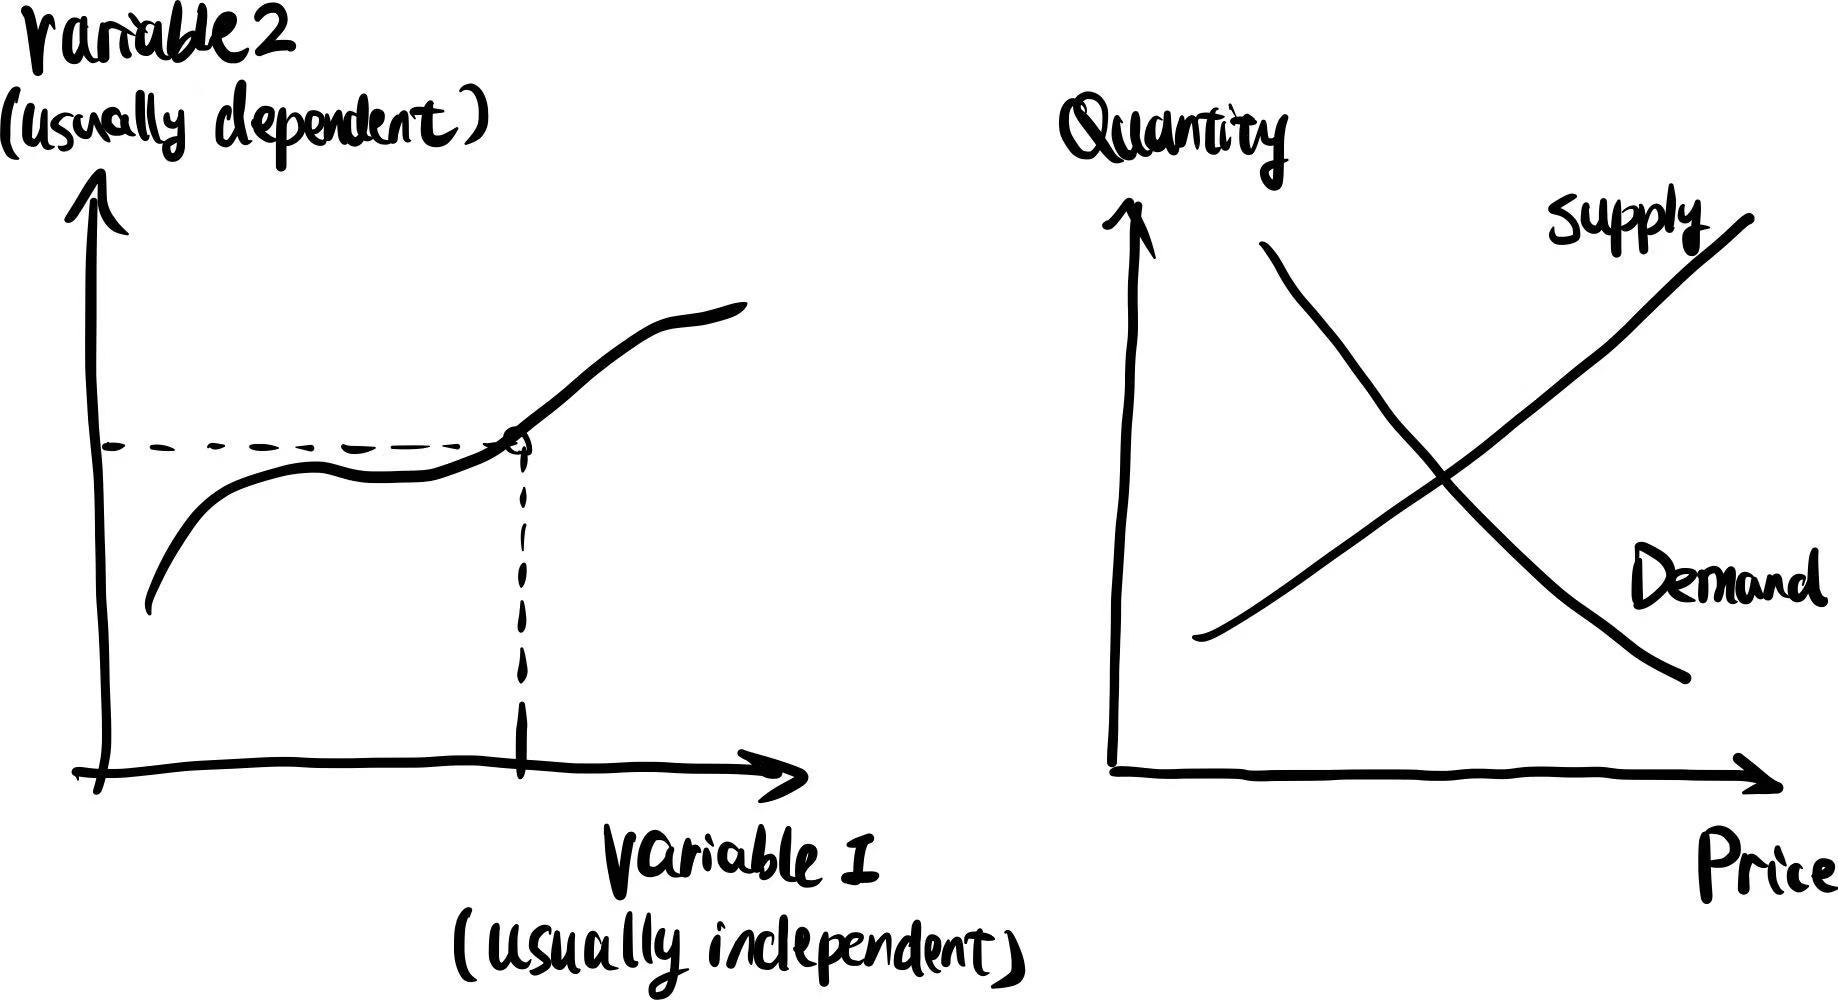
\includegraphics[width=0.9\textwidth]{img/image-20230228095149998.png}

\kaishu{\small 随着某商品的市场价格 (price) 增高, 生产者的生产意愿自然是增高的,
因为不考虑成本和其他因素变化的情况下 (Ceteris Paribus),
多生产的利润会更高, 因此供给曲线 (supply) 上扬, 反映出价格和供给量
(supply quantity) 的正相关; 另一方面,
消费者的消费意愿随着价格上涨自然是下降的, 于是需求曲线 (demand) 下压,
反映出价格和需求量 (demand quantity) 的负相关.

两条曲线分别对应着供给量和需求量关于价格的函数,
两函数的焦点反映了理想的自由市场下的最终成交价格和供需量
(因为在这个点达到了供需平衡 - equilibrium) ,
焦点向下作竖直线与横轴的焦点便显示了最终成交价格,
焦点向左作水平线与竖轴的交点便显示了平衡点的供需量.}
\end{tcolorbox}

在工程和计算机科学等思维里, 函数更像下左图所示, 给定一个输入 (input),
函数如同一台机器, 在加工后给出一个输出 (output); 这台机器非常可靠,
同样的输入能够稳定输出同样结果. 下右图给了一个例子

\begin{tcolorbox}[size=fbox, breakable, enhanced jigsaw]

\includegraphics[width=0.9\textwidth]{img/image-20230228095405809.png}

\kaishu{\small 假想有这样一个叫做``首都'' (Captital) 的函数,
放入一个国家名便会稳定输出这个国家的首都,
数学上我们可以这么标记下右图的例子 $\text{Capital(China)=Beijin}$.}
\end{tcolorbox}

函数的近现代定义和工科思维里的图景就很像, 考虑集合 $X$ 和 $Y$,
且它们不是空的, 如果存在某种特定的对应关系 $f$, 使得对于 $X$
中任意一个元素 $x$, 在 $Y$ 中都有唯一确定的元素 $y$ 和 $x$ 对应,
那么就称\textbf{映射} (mapping)\footnote{~Mapping 这个词用在这很贴切,
  map有地图的意思,
  ``映射''和地图上的每个点对应着实际区域上的一个个位置很相似.}
$f: A\rightarrow B$ 为从 $X$ 到 $Y$ 的一个函数, 记作
$y=f(x), x\in X$ 或者 $f(X)=\{y|f(x)=y, y\in Y\}$;
第一种记法强调元素的映射, 第二种记法强调整个集合的映射, $X$
在这里便是这个映射的定义域, $f(X)$ 是值域, $Y$
是这个映射的\textbf{陪域} (codomain, 也叫做上域, 到达域, 对应域),
大括号表示 $X$ 被映射到的集合, 其元素 $y$ 满足竖线后的条件, 即 $y$
是自 $x$ 通过 $f$ 这个映射得到, 并且 $y$ 属于 $Y$.
这样定义的直观感受类似下左图, 之前``首都''函数便类似下右图

\begin{tcolorbox}[size=fbox, breakable, enhanced jigsaw]
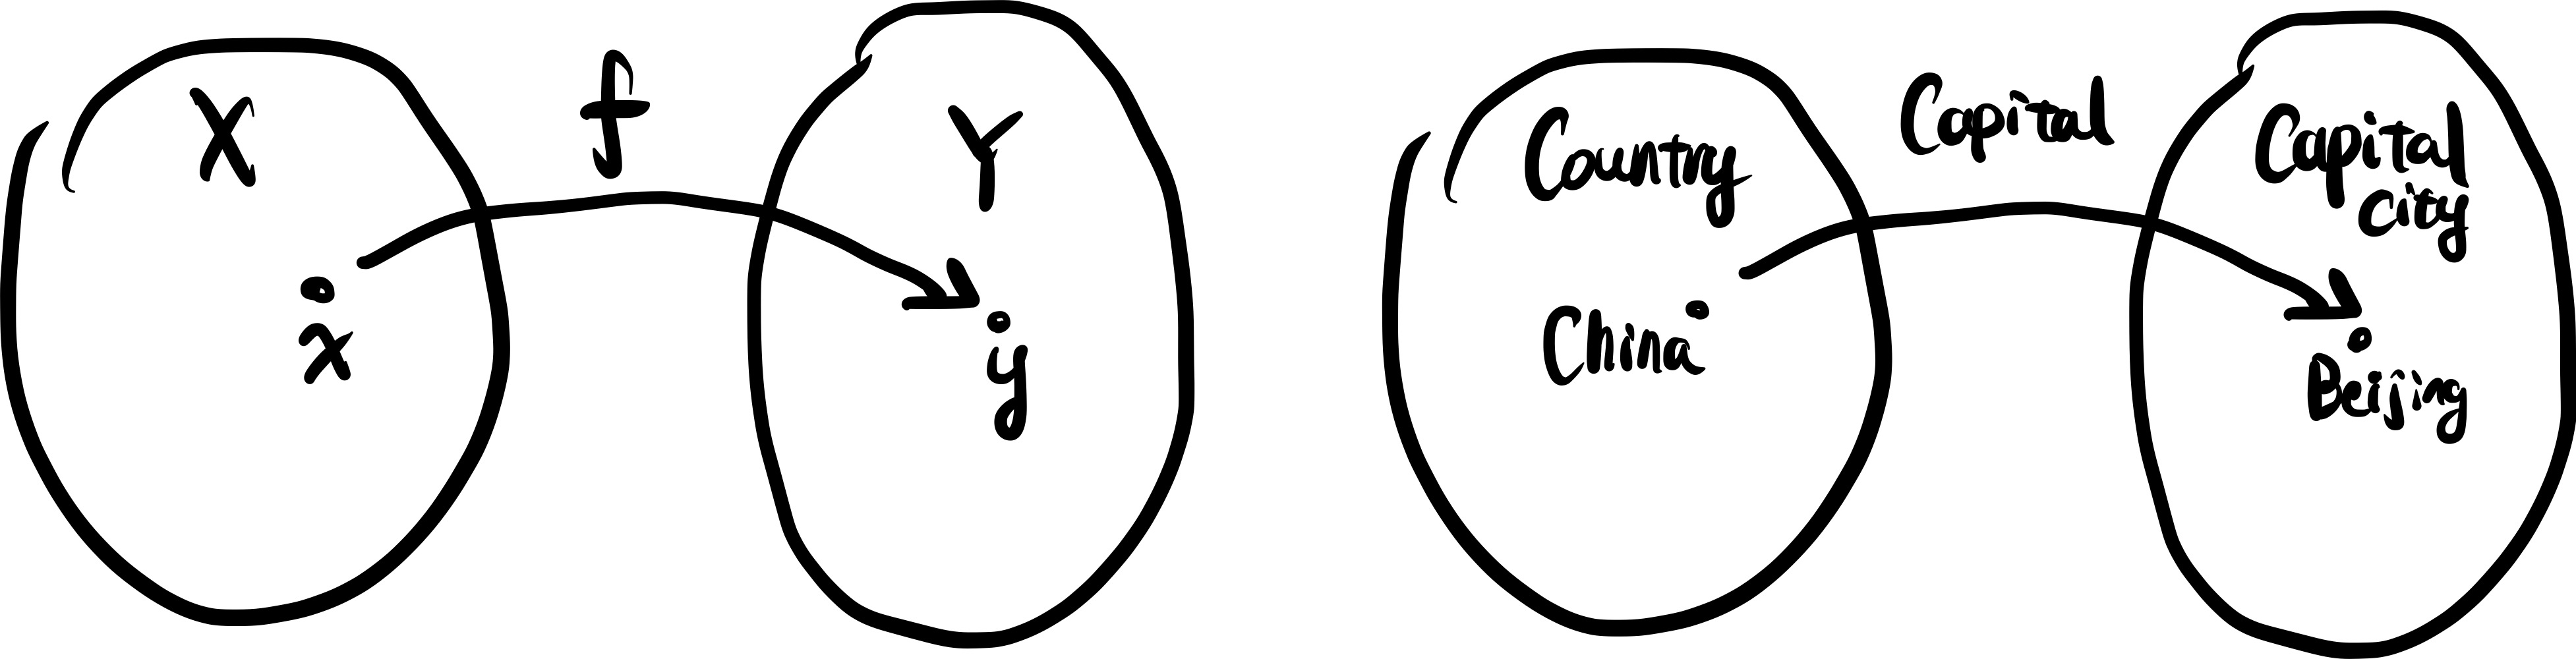
\includegraphics[width=0.9\textwidth]{img/image-20230228112941902.png}

\kaishu{\small Country这个集合里包含了很多国家, \{中国, 美国, 日本, \ldots\}; Capital
city这个集合里包含了很多城市, \{北京, 华盛顿, 东京, \ldots\};
Capital这个函数便描述了Country中的元素和Capital city中的元素的对应关系.}
\end{tcolorbox}

\end{tcolorbox}
\section{函数-下}\label{004}

\begin{flushright}{\kaishu 無名, 天地之始; 有名, 萬物之母. 常無, 欲以觀其妙; 常有, 欲以觀其徼. \\- 苏辙 『老子解』}\end{flushright}

\begin{tcolorbox}[size=fbox, breakable, enhanced jigsaw, title={单射, 满射, 双射 (injection, surjection,
bijection)}]

一个函数 $f:X\rightarrow Y$ 若满足, 如果 $a\neq b$ 则
$f(a)\neq f(b)$ 对于任何属于 $X$ 的 $a$ 和 $b$,
那么它便是\textbf{单射}的 (injection, one-to-one)\footnote{One-to-one
  是更``纯正''英语的说法, 比较通俗, injection 是来自法语的舶来词,
  更具高级感; 后面的 onto 和 surjection 同.}.

一个函数 $f:X\rightarrow Y$ , 若它的值域 (range) 和陪域 (codomain)
一致, 即对于任意 $y\in Y$, 都存在至少一个 $x\in X$ 满足
$f(x)=y$\footnote{介绍一下符号语言: $\exists$ - 存在; $\forall$ -
  对于所有. 于是这句话可以这么表述:
  $\forall y\in Y, \exists x\in X \text{ s.t. } f(x)=y$ (s.t.=such that
  可以译为``使得''). 但是通常情况下,
  还是尽量避免符号语言而使用自然语言来描述.}, 那么它便是\textbf{满射}的
(surjection, onto).

一个同时单射又满射的函数是\textbf{双射}的 (bijection, one-to-one
correspondance).

还是以Captial这个函数为例子, 下面给出了单射, 满射,
双射三种情况分别的图示:

\begin{tcolorbox}[size=fbox, breakable, enhanced jigsaw]
\begin{center}
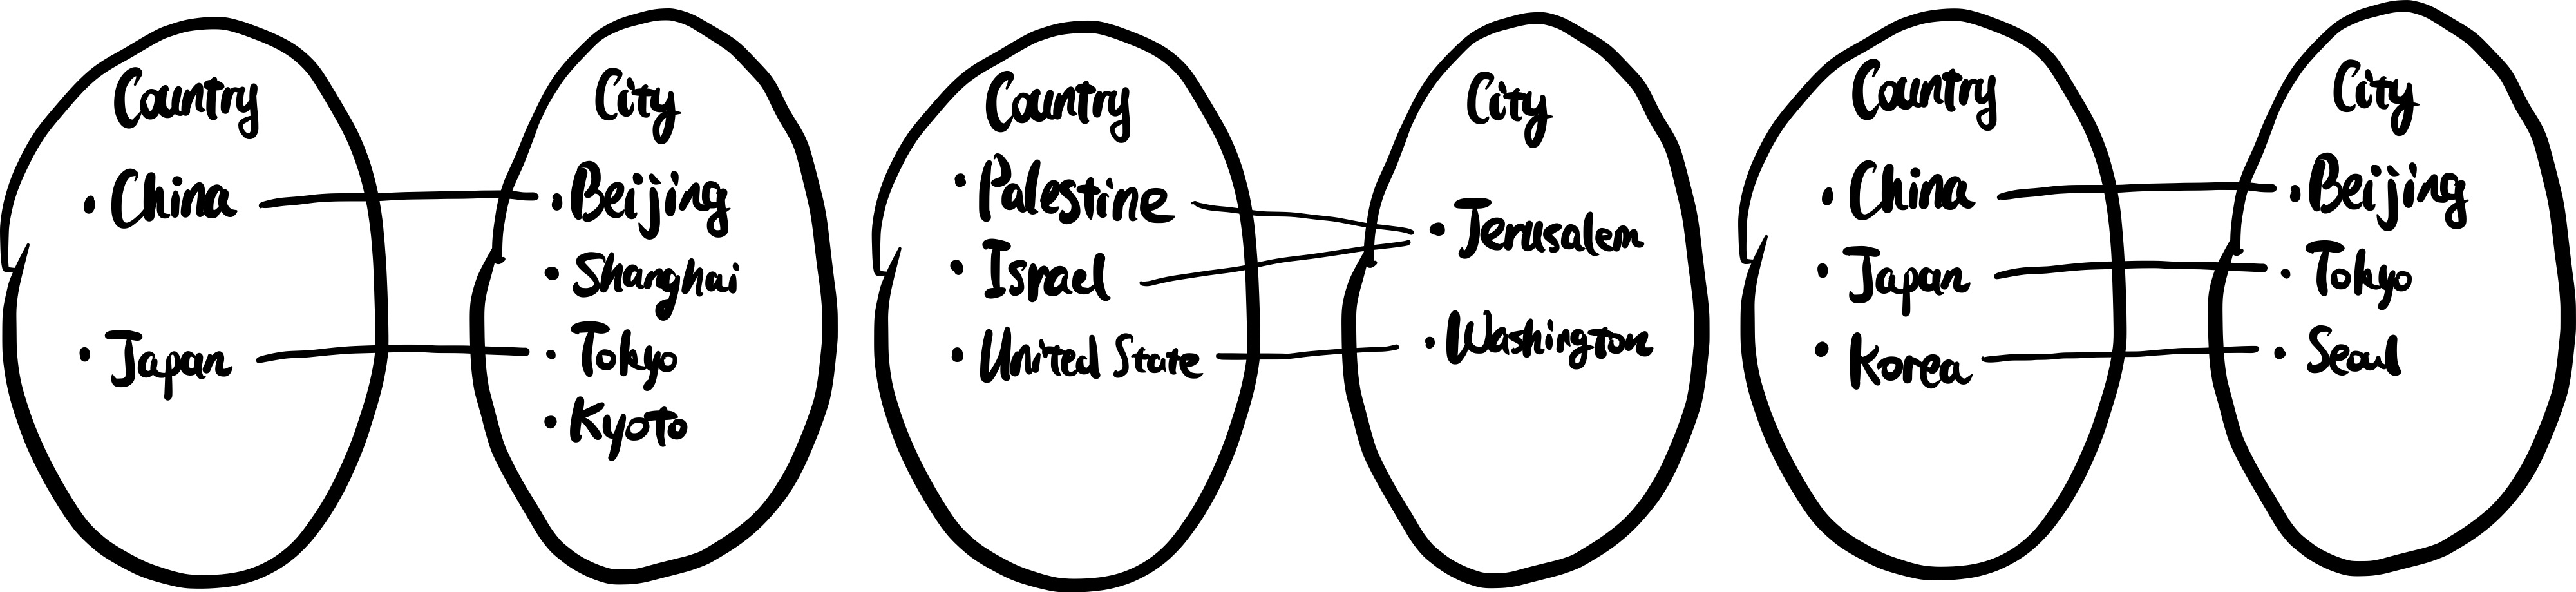
\includegraphics[width=0.9\textwidth]{img/image-20230302091706069.png}
\end{center}

\kaishu{\small 左: 单射但不满射; 中: 满射但不单射; 右: 双射.}
\end{tcolorbox}

\end{tcolorbox}

\begin{tcolorbox}[size=fbox, breakable, enhanced jigsaw, title={奇偶性 (parity 大嘘)}]

若一个函数满足 $f(-x)=-f(x)$, 即改变输入值 (自变量) 的正负号, 输出值
(因变量) 的正负号也改变, 这个函数便是\textbf{奇函数} (odd function).
图像上它是关于原点对称的.

若一个函数满足 $f(-x)=f(x)$, 即改变输入值 (自变量) 的正负号,
不影响输出值 (因变量) , 这个函数便是\textbf{偶函数} (even function).
图像上它是关于 $y$ 轴对称的.

当然, 奇函数和偶函数事实上是很特殊的两类函数,
更多的函数既不是奇函数又不是偶函数.

一些运算规律:

\begin{itemize}

\item
  奇函数 + 奇函数 = 奇函数\\{\kaishu 证明}: 假设存在两个奇函数 $f(x)$ 和
  $g(x)$, 令 $(f+g)(x) := f(x) + g(x)$, 即 $(f+g)(x)$
  这个函数是原本两函数之和. 根据奇函数的定义, $f(-x)=-f(x)$ 且
  $g(-x)=-g(x)$, 将两式相加得 $f(-x)+g(-x)=-f(x)-g(x)$, 即有
  $(f+x)(-x)=-(f+g)(x)$, 可见 $(f+g)(x)$ 是奇函数.
\item
  偶函数 + 偶函数 = 偶函数\\本条及接下来的证明与上一条类似, 可以当作练习.
\item
  奇函数 ×/÷ 奇函数 = 偶函数
\item
  偶函数 ×/÷ 偶函数 = 偶函数
\item
  奇函数 ×/÷ 偶函数 = 奇函数
\item
  偶函数 ×/÷ 奇函数 = 奇函数
\end{itemize}

\end{tcolorbox}

\begin{tcolorbox}[size=fbox, breakable, enhanced jigsaw, title={反函数 (inverse
function)}]

浅浅地非专业地叙述一下反函数. 设函数 $y=f(x)\ (x\in X)$ 的值域是
$Y$, 若存在一个函数 $g(y)$ 使得 $x= g(y)\ (y\in C)$, $g(x)$
便叫做 $f(x)$ 的\textbf{反函数} (inverse function), 可以记作
$x=f^{-1}(y)$, 它的定义域和值域分别是原函数的值域和定义域。

图像上, 反函数和原函数关于 $y=x$ 对称.

在求反函数时要特别注意反函数与原函数的定义域和值域. 例如 $y=f(x)=x^2$,
因为 $(\pm x)^2=y$, 反函数可能是 $x=f^{-1}(y)=\sqrt{y}$ 也可能是
$x=f^{-1}(y)=-\sqrt{y}$ , 但是不能是 $x=f^{-1}(y)=\pm\sqrt{y}$,
因为这样便不符合函数定义了, 一个输入值不可以有多个输出值,
或则说一个自变量不能对应多个因变量
(但是多个因变量对应一个自变量是允许的, 可以参考满射但不单射的图例).
这里反函数取正或负取决于原函数的定义域, 若 $y=f(x)=x^2, x\ge 0$, 则
$x=f^{-1}(y)=\sqrt{y}$; 若 $y=f(x)=x^2, x\le 0$, 则
$x=f^{-1}(y)=-\sqrt{y}$.

\end{tcolorbox}

\begin{tcolorbox}[size=fbox, breakable, enhanced jigsaw, title={隐函数 (implicit
function)}]

有的时候可能需要用函数来表达一个比较复杂的图像, 举一个简单一点的例子,
一个圆心位于原点的单位圆, 圆上任意一点到圆心距离都是 $1$, 于是有
$x^2+y^2=1$, 用前面学习的函数的形式表达这个关系, 有

$y=\begin{cases}\sqrt{1-x^2}\\-\sqrt{1-x^2}\end{cases}.$

这样似乎还没有起先的 $x^2+y^2=1$ 这个形式美观, 因此不妨还是用
$x^2+y^2-1=0$ 来表述单位圆上的 $x$ 与 $y$ 的关系. 类似这样,
利用一个【同时关于 $x$ 与 $y$ 的表达式 $F(x,y)=0$】来确定【 $y$
关于 $x$ 的函数】的表达式, 我们称之为\textbf{隐函数} (implicit
function); 为表区分, 前面介绍的类似 $y=f(x)$ 的函数,
称为\textbf{显函数} (explicit function).

\end{tcolorbox}

\begin{tcolorbox}[size=fbox, breakable, enhanced jigsaw, title={线性 (linearity)}]

这是一个很好的特性, 并不局限于函数, 仅对于函数来说的话,
若一个函数是线性的, 便有

$f(a+b)=f(a)+f(b),\ f(ax)=af(x).$

\end{tcolorbox}
\section{三角函数}\label{005}

\begin{flushright}{\kaishu 道可道, 非常道; 名可名, 非常名.}\end{flushright}

\begin{tcolorbox}[size=fbox, breakable, enhanced jigsaw, title={三角函数
(trigonometry)}]

三角函数最基本的使用应该是表示直角三角形的变长比. 如下图所示, 三角形
$ABC$ 为直角三角形, 将 $\angle BAC$ 记作 $\theta$, 对于两条直角边
$AB$ 和 $BC$, 边 $AB$ 在 $\theta$ 边上, 称它为\textbf{邻边}
(adjacent), 边 $BC$ 在 $\theta$ 对面, 称它为\textbf{对边}
(opposite), 剩余的边 $AC$ 被称为\textbf{斜边} (hypotenuse)。

\begin{tcolorbox}[size=fbox, breakable, enhanced jigsaw]
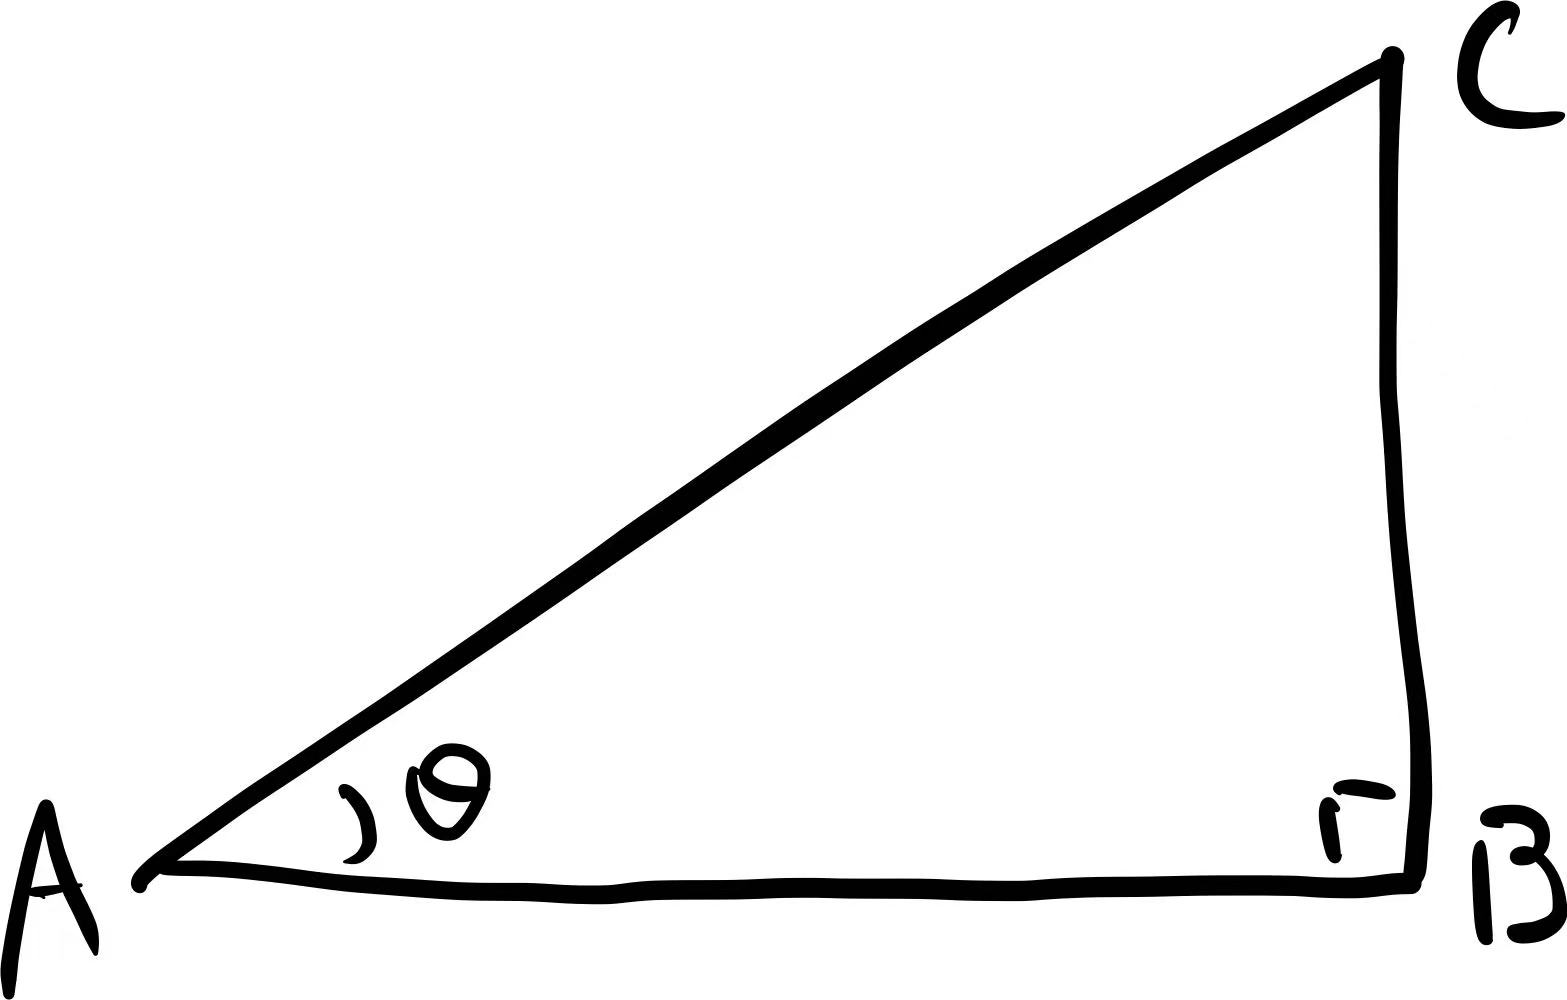
\includegraphics[width=0.5\textwidth]{img/image-20230308142717670.png}
\end{tcolorbox}

易见, 各变长比仅和 $\theta$ 相关\footnote{当然也可以说和除了直角外的另一个角
  $(90^\circ-\theta)$ 相关; 边长比可以通过一个除直角外的角确定是因为,
  除直角外另一角相等的直角三角形都相似, 它们的边长比是一致的。},
三角函数便是用来表示各个比例的, 常用的三角函数有

$\begin{aligned}\cos\theta&=\frac{\text{邻边}}{\text{斜边}}=\frac{AB}{AC},\\ \sin\theta&=\frac{\text{对边}}{\text{斜边}}=\frac{BC}{AC},\\ \tan\theta&=\frac{\text{对边}}{\text{邻边}}=\frac{BC}{AB}.\end{aligned}$

不难看出$\tan\theta=\frac{\sin\theta}{\cos\theta}$.

另外还有

$\begin{aligned}\sec\theta&\equiv\frac{1}{\sin\theta},\\ \csc\theta&\equiv\frac{1}{\cos\theta},\\ \cot\theta&\equiv\frac{1}{\tan\theta}.\end{aligned}$

$\csc$ 很多时候也记作 $\text{cosec}$.

一个非常实用的关系, 直角三角形中有\textbf{勾股定理} (Pythagorean
theorem): 斜边边长平方等于两直角边边长的平方之和, 即 $AC^2=AB^2+BC^2$;
两边同时除以 $AC^2$ 便有

\begin{itemize}

\item
  $\boxed{1=\cos^2\theta+\sin^2\theta}$.\footnote{三角函数的平方:
    cos(x)\textsuperscript{2} 通常理解为 cos((x)\textsuperscript{2});
    cos\textsuperscript{2}x 约定俗成表示 (cos(x))\textsuperscript{2}.}
\end{itemize}

\end{tcolorbox}

\begin{tcolorbox}[size=fbox, breakable, enhanced jigsaw, title={反三角函数}]

三角函数, 输入一个角度, 返回一个边长比; 反三角函数便是三角函数得逆运算,
或者说反函数 (参见【\ref{004}\nameref{004}】), 即输入一个边长比, 返回一个角度.

\end{tcolorbox}

\begin{tcolorbox}[size=fbox, breakable, enhanced jigsaw, title={正弦定律 (law of sine)}]

将三角形三个角分别记作 $\alpha$, $\beta$, 和 $\gamma$,
将它们的对边分别记作 $A$, $B$, 和 $C$. 先是结论:

\begin{itemize}

\item
  $\boxed{\frac{A}{\sin\alpha}=\frac{B}{\sin\beta}=\frac{C}{\sin\gamma}}$.
\end{itemize}

\begin{tcolorbox}[size=fbox, breakable, enhanced jigsaw]
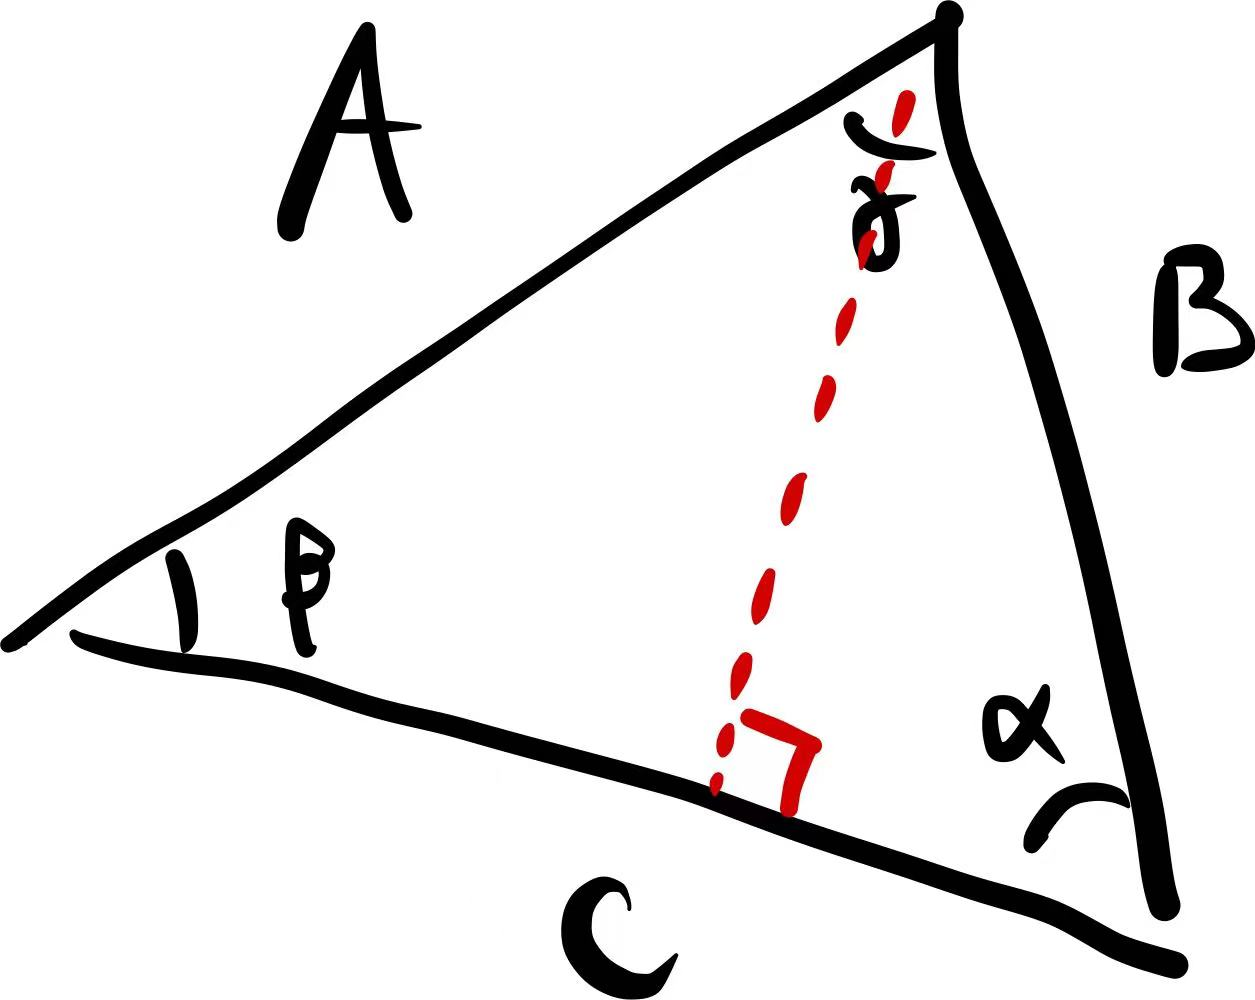
\includegraphics[width=0.5\textwidth]{img/image-20230308142913522.png}
\end{tcolorbox}

推导如下:

如上图所示, 以 $C$ 为底做高, 将原本的三角形分为左右两个直角三角形,
这条高利用左边的直角三角形可以表示为 $A\sin\beta$,
利用右边的直角三角形则是 $B\sin\alpha$, 于是有
$A\sin\beta=B\sin\alpha$, 整理可得
$\frac{A}{\sin\alpha}=\frac{B}{\sin\beta}$;
再做另一条高重复前面的操作, 便可得到完整的结论.

\end{tcolorbox}

\begin{tcolorbox}[size=fbox, breakable, enhanced jigsaw, title={余弦定律 (law of cosine)}]

还是先上结论:

\begin{itemize}

\item
  $\boxed{B^2=A^2+C^2-2AC\cos\beta}$,
\end{itemize}

即, 【一条边的边长平方】等于【另两条边的边长平方之】和加上【两倍的
(另两条边边长的乘积) 乘以 (另两条边的夹角的余弦)】.

\begin{tcolorbox}[size=fbox, breakable, enhanced jigsaw]
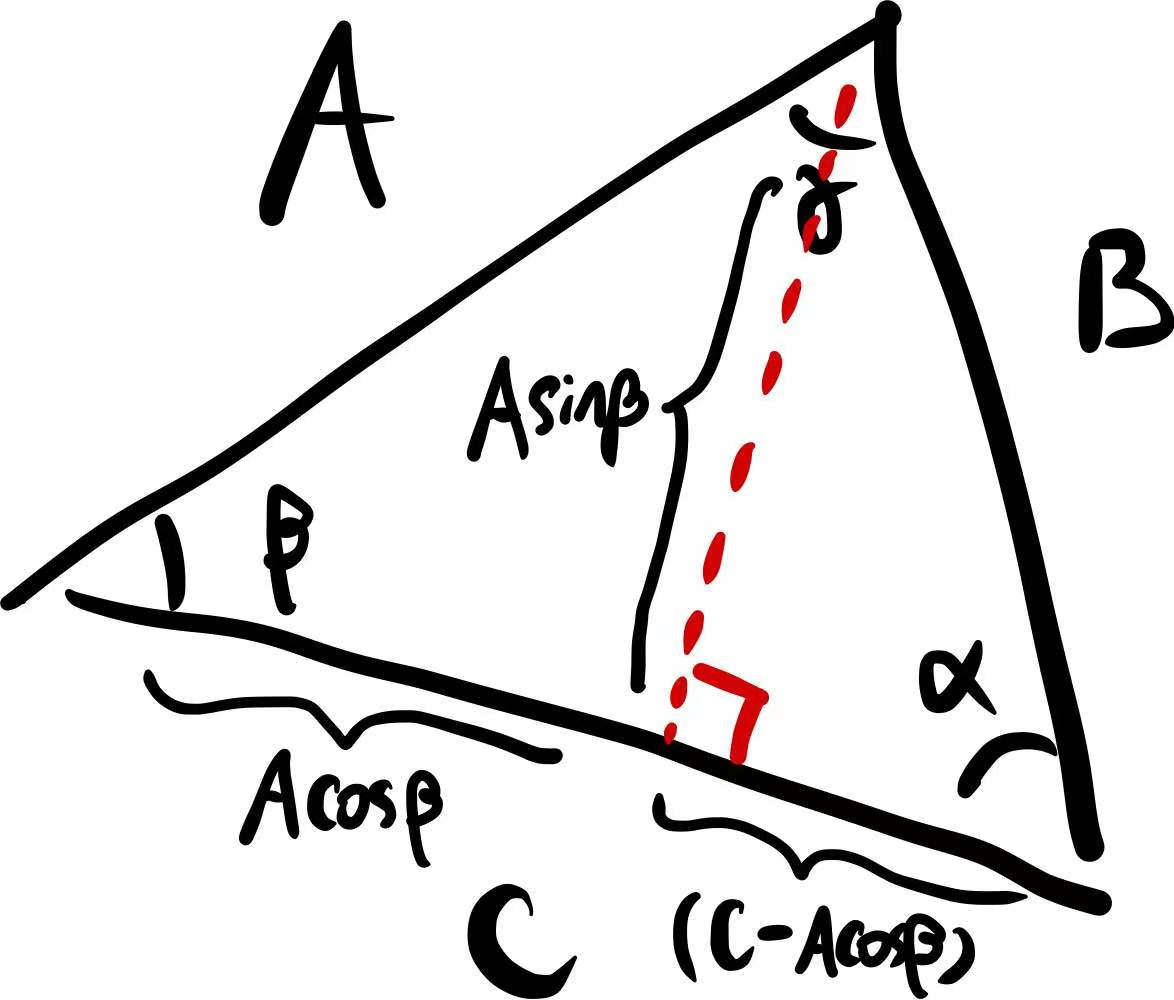
\includegraphics[width=0.5\textwidth]{img/image-20230308151417631.png}
\end{tcolorbox}

推导如下:

如下图所示, 依旧利用底边 $C$ 上的高将其分为左右两个直角三角形;
左边的直角三角形, 利用斜边 $A$ 和角 $\beta$, 两直角边分别可以表示为
$A\cos\beta$ 和 $A\sin\beta$, 于是右边的直角三角形边长便可表述为
$A\sin\beta$ 和 $(C-A\cos\beta)$; 对右边的直角三角形使用勾股定理

$\begin{aligned}B^2&=A^2\sin^2\beta+(C-A\cos\beta)^2\\ &=A^2\sin^2\beta+C^2+A^2\cos^2\beta-2AC\cos\beta\\ &=A^2+C^2-2AC\cos\beta.\end{aligned}$

其中等式的后两行用到了之前得出的 $1=\cos^2\theta+\sin^2\theta$.

\end{tcolorbox}

\begin{tcolorbox}[size=fbox, breakable, enhanced jigsaw, title={任意角度的三角函数}]

不难发现, 前面讨论的情况似乎都是锐角的情况 (主要是因为插图\ldots),
钝角的三角函数似乎没那么直观了, 因为做不成一个含有钝角的直角三角形,
没法简单地用边长比来表示 $\sin$ 和 $\cos$ 等. 于是,
我们需要想办法将前面的情形推广.

如下左图所示, 建立直角坐标系, 做一圆心位于原点的单位圆, 即半径为 $1$
的圆, 考虑在第一象限的圆上的一点, 将其与原点做连线, 将从
$x$-轴正方向与这条连线\textbf{顺时针}方向形成的夹角记作 $\theta$,
不难看出这个点的坐标 $(x,y)$ 满足

$\begin{cases}x=\cos\theta,\\y=\sin\theta.\end{cases}$

\begin{tcolorbox}[size=fbox, breakable, enhanced jigsaw]
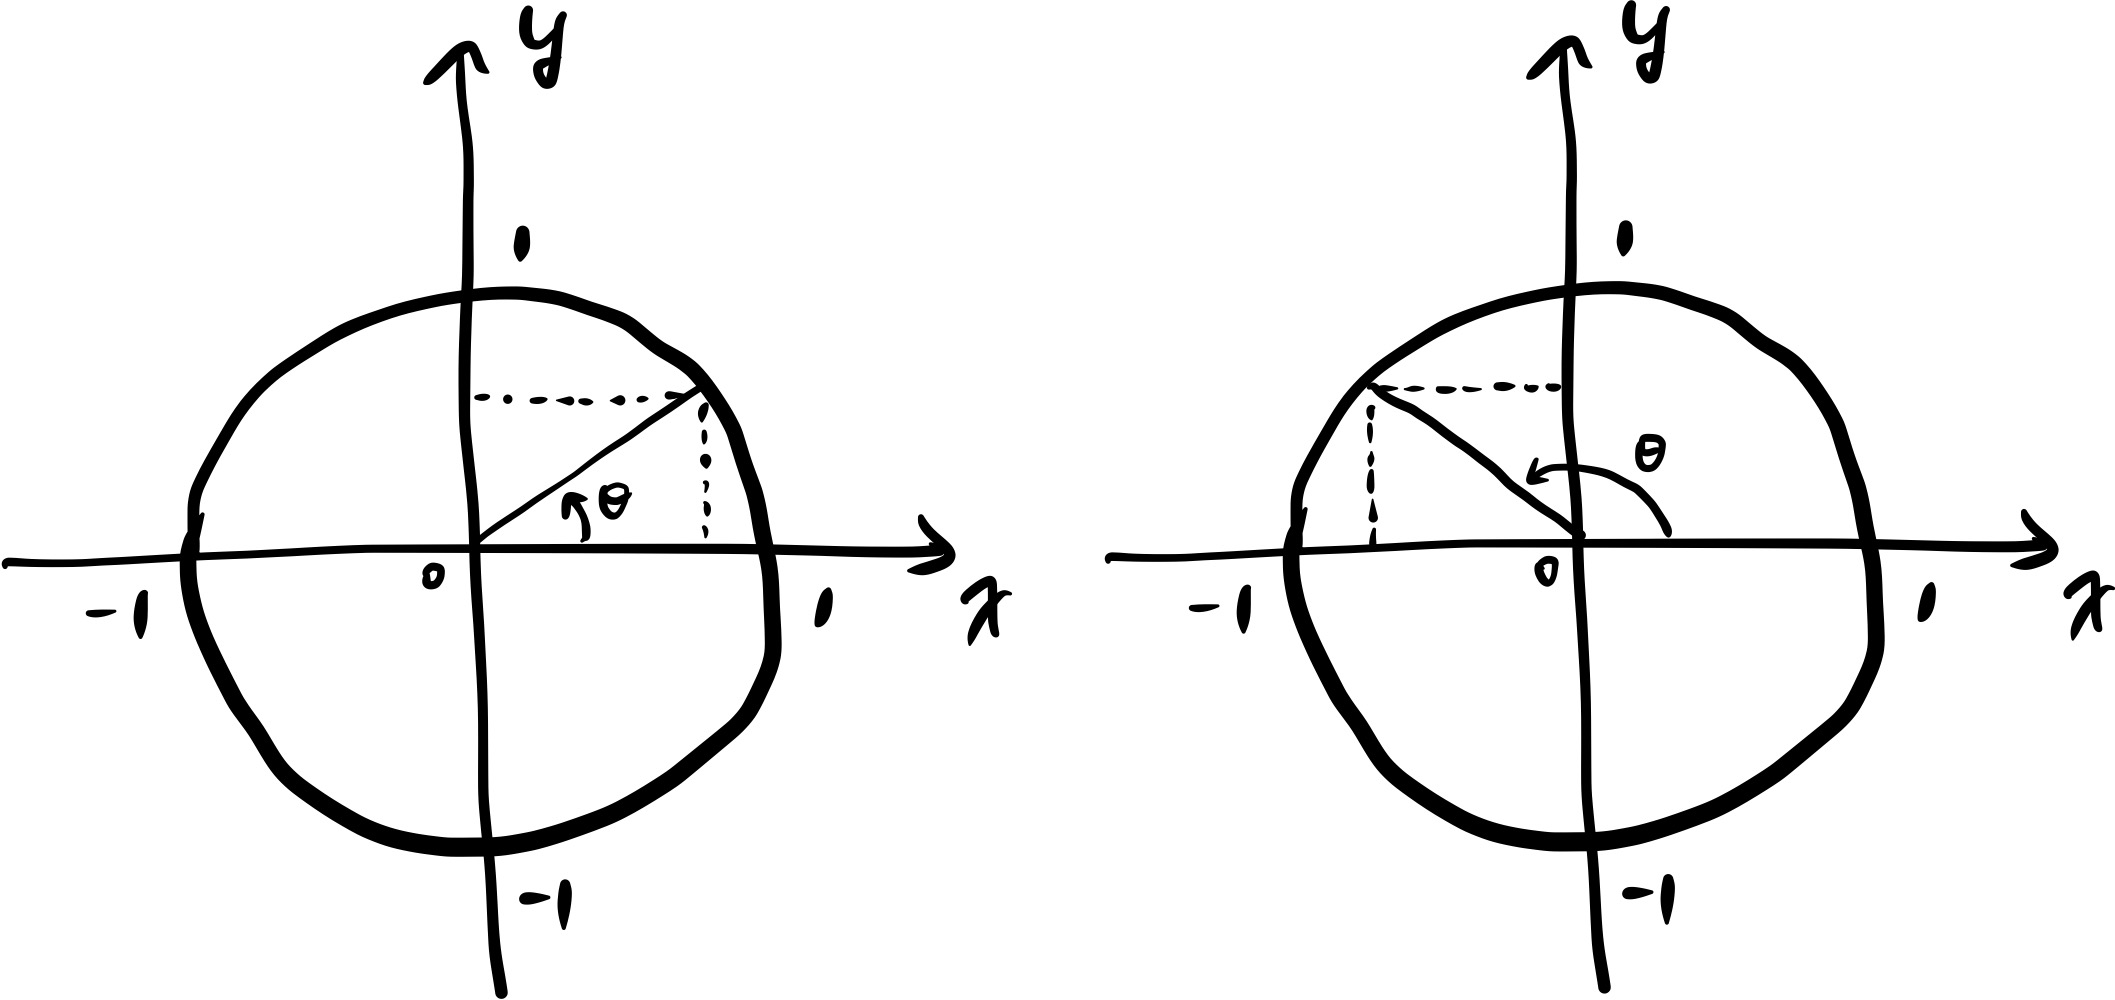
\includegraphics[width=0.75\textwidth]{img/image-20230316171124433.png}
\end{tcolorbox}

于是不妨将其他象限的情况也按此定义,
于是如上右图所示的钝角甚至更大角度的三角函数便可以被定义了.

\end{tcolorbox}

\begin{tcolorbox}[size=fbox, breakable, enhanced jigsaw, title={弧度制 (radian)}]

为什么一个周角是 $360^\circ$ 呢, 听说过一个不可考的说法: $360$
是一个有很多因数的数字 (1, 2, 3, 4, 5, 6, 8, 9, 10, 12\ldots),
等分起来的时候数字会比较友好, 所以 $360^\circ$ 其实是非常随意地规定的.
那么有没有更好的用来描述角度方法呢? 答案是弧度.

一个半径为 $r$ 的圆的周长是 $2\pi r$, 一个圆心角为 $n^\circ$
的扇形的弧长是 $2\pi r\frac{n}{360}$. 可见圆心角越大弧越长,
且圆心角和弧长成正比. 既然如此,
不如重新将角度定义为圆心角与弧长的比值以方便计算, 于是便有了,
在新的这套单位系统中, 若圆心角大小为 $\theta$, 其对应弧长应为
$r\theta$; 当圆心角是一个周角时, 对应弧长便成了圆的周长 $r(2\pi)$.
所以角度和这个新的单位的换算有 $360^\circ\equiv 2\pi\ \text{rad}$,
因为这个单位把圆心角和对应的弧长联系起来了, 因此称之为\textbf{弧度}
(radian).

扇形面积在这套单位制, 即弧度制下, 便也成了 $\frac{1}{2}r^2\theta$.

\end{tcolorbox}

\begin{tcolorbox}[size=fbox, breakable, enhanced jigsaw, title={三角函数的图像}]

现在这个时代, 大家都或多或少能接触到科学计算器,
再不济在bing.com上搜索``solver''用微软的 Microsoft Solver
也可以计算某个特定角度的三角函数值, 自然也可以绘制函数图像.
下图分别展示了 $\sin(x)$ 和 $\cos(x)$ 的图像,

\begin{tcolorbox}[size=fbox, breakable, enhanced jigsaw]
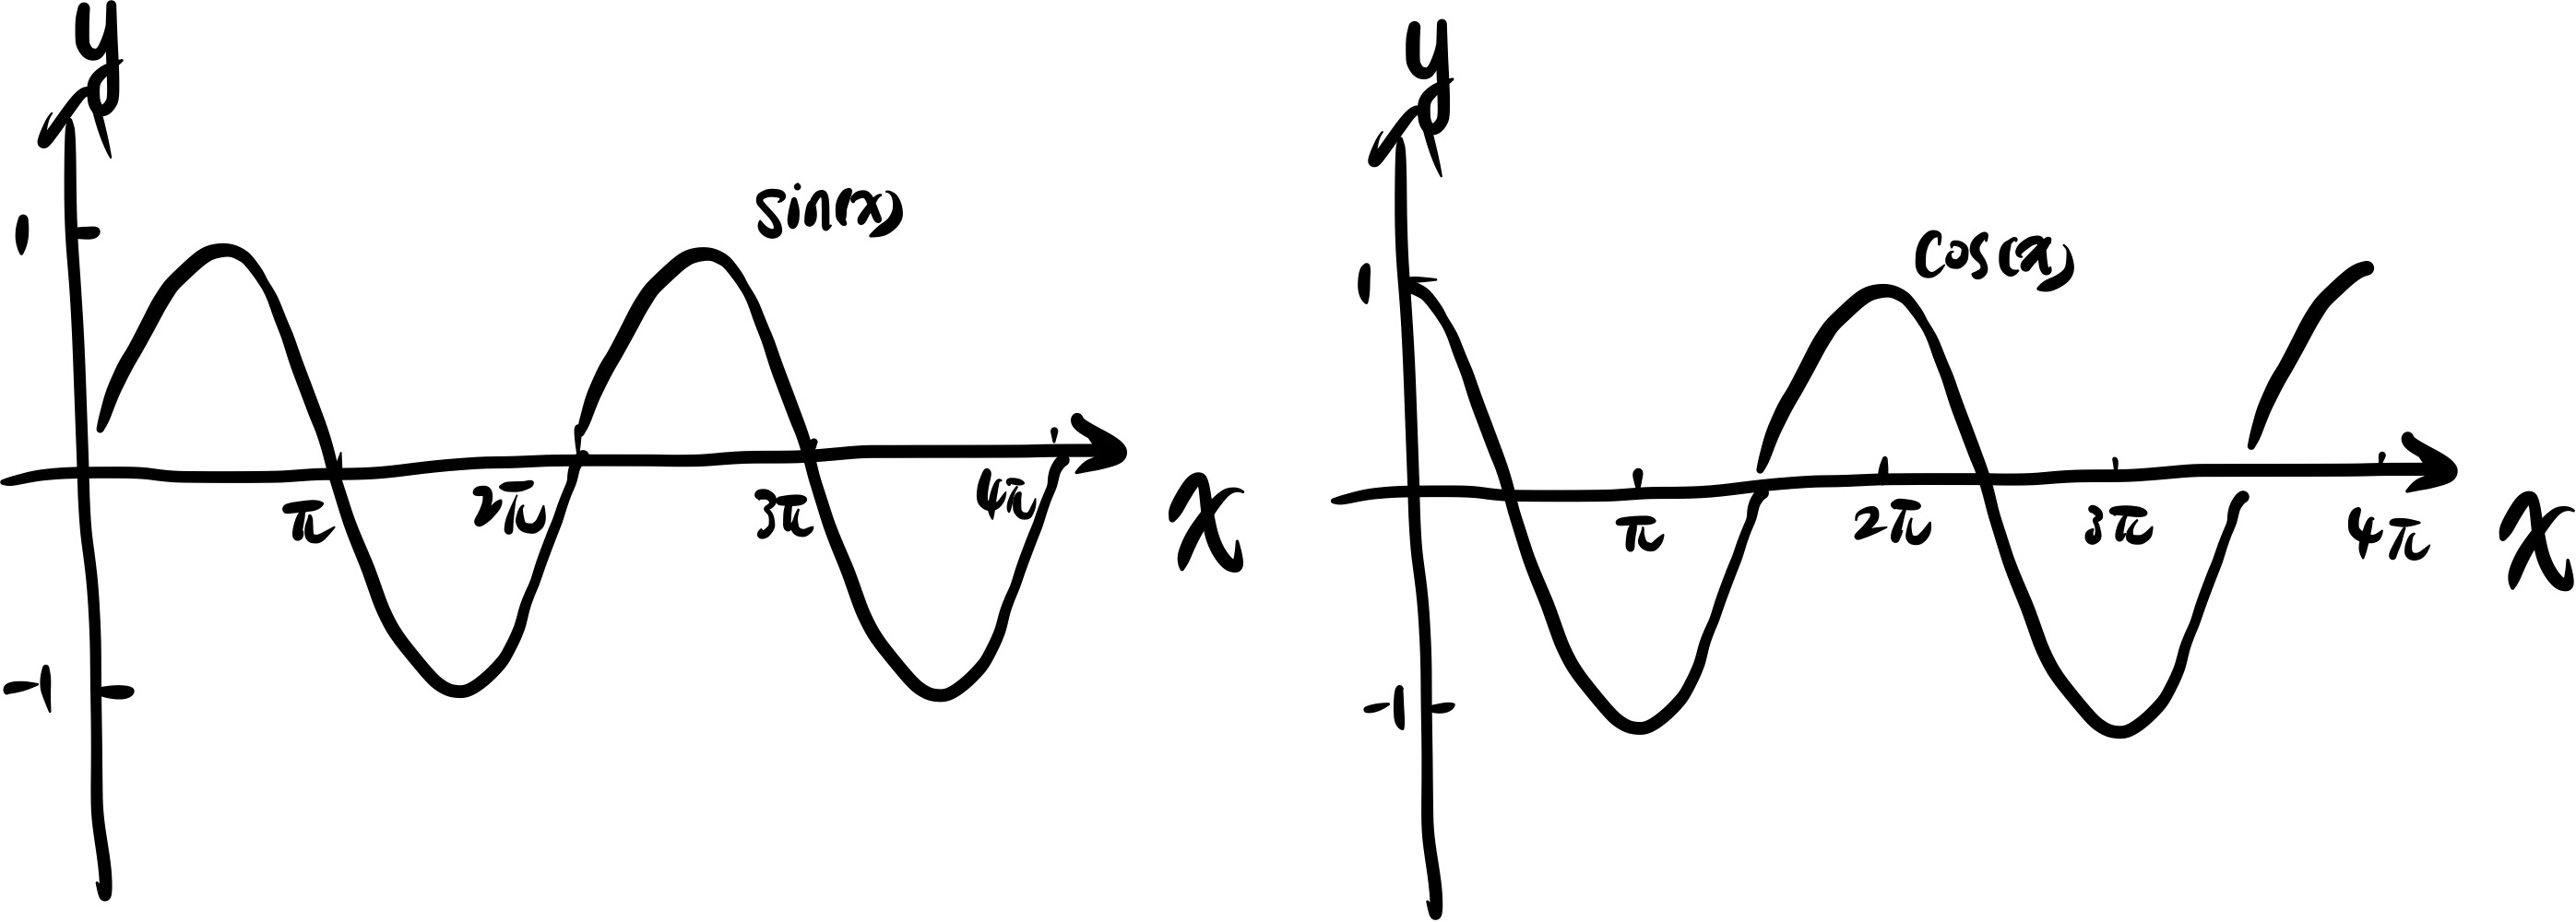
\includegraphics[width=0.75\textwidth]{img/image-20230316171137500.png}
\end{tcolorbox}

一些值得关注的点是它们都是\textbf{周期函数} (periodic function),
随着自变量-角度的变化, 因变量-函数值的变化是周期性的, 它们的周期都是
$2\pi$, 这一点从上文的单位圆里便可看出些许原因,
当角度变化超过一个周角时, 和角度刚从 $0$ 开始的情况是一样的.

\end{tcolorbox}
\section{虚数和复数}\label{006}

\begin{flushright}{\kaishu 些许绕行 (detour).}\end{flushright}

\begin{tcolorbox}[size=fbox, breakable, enhanced jigsaw, title={虚数和复数 (imaginary number and complex number)}]

考虑一个一元二次方程 $ax^2+bx+c=0$, 它的解有

$\begin{aligned}
0&=a\left(x^2+\frac{b}{a}x+\frac{c}{a}\right)\\
0&=x^2+\frac{b}{a}x+\frac{c}{a}\\
0&=x^2+\frac{b}{a}x+\left(\frac{b}{2a}\right)^2-\left(\frac{b}{2a}\right)^2+\frac{c}{a}\\
0&=\left(x-\frac{b}{2a}\right)^2-\left(\frac{b}{2a}\right)^2+\frac{c}{a}\\
\left(x-\frac{b}{2a}\right)^2&=\left(\frac{b}{2a}\right)^2-\frac{c}{a}\\
&...\\
x&=\boxed{\frac{-b\pm\sqrt{b^2-4ac}}{2a}}.
\end{aligned}$

上式最后的结论便是求根公式, 不难看出整个推导过程实际上就是配方,
其中根号前面的``加减''是因为对等式两边同时开方时,
正负两种情况都是正确的.

我们在此之前接触到的数字都还限于实数范围内, 因此会要求
$\left(b^2-4ac\right)$ 是正的, 以保证开方之后的结果是``有意义的'',
然而

\begin{newquote}
    ``从来如此, 便对么?''
\end{newquote}

之前也出现了, 不能被表示成分数形式的数字,
我们的研究范围从有理数扩充到了实数; 现在, 若 $\left(b^2-4ac\right)$
是负的, 按照当前的理解, 它不能被开方, 那是不是又到了这样一个神圣的时刻,
我们需要拓展我们研究的数字的范围?

既然如此, 不如规定 $\sqrt{-1}\equiv i$, 作为新的一类数字的单位,
因为之前的数字叫``实数'', 那么这一类新的数字就不妨叫做``\textbf{虚数}''
(imaginary number) 吧. 一个既包含实数部分, 又包含虚数的部分的数字,
我们就叫它``\textbf{复数}'' (complex number), 记作 $\mathbb{C}$.
\end{tcolorbox}

\begin{tcolorbox}[size=fbox, breakable, enhanced jigsaw, title={运算规律}]

考虑若干个复数, $z_1=a+bi$, $z_2=c+di$, $z_3=e+fi$\ldots{}

\begin{itemize}

\item
  \textbf{加法}: $z_1+z_2=(a+c)+(b+d)i$.
  实数部分和虚数部分可以分开计算,
  应该不难看出复数和加法是构成\textbf{阿贝尔群}的
  (即它具有封闭性和结合律, 有单位元和逆元, 并且有交换律, 详细参见\ref{001}\nameref{001}).
\item
  \textbf{乘法}:
  $z_1\times z_2=(a+bi)\times(c+di)\\=ac+adi+bci+bdi^2=(ac-bd)+(ad+bc)i.$
  不难看出, 复数和乘法也构成阿贝尔群.
\item
  乘法对于加法满足\textbf{分配律}, 即,
  $(z_1+z_2)\times z_3=z_1\times z_3+z_2\times z_3$,
  证明留作练习\footnote{事实上, 很多情况下, 之前提到的很多知识点,
    例如单位元, 零元, 逆元都分左右, 分配律也有左分配律和右分配律,
    但是目前讨论的情况都是满足交换律的, 所以可以不区分左右.}.
\end{itemize}

以上三条已经足够使得复数与加法和乘法构成一个\textbf{环} (ring), 事实上,
环只需要乘法是半群 (semi-group, 即满足结合律和有单位元的二元运算与集合) 即可.

\begin{itemize}

\item
  \textbf{减法}: 因为加法存在逆元, 所以减去一个数,
  可以视作加上这个数的加法逆元, 即:
  $z_1-z_2=(a+bi)-(c+di)\\\Rightarrow z_1+(-z_1)=(a+bi)+(-(c+di))=(a-c)+(b-d)i$
\item
  \textbf{除法}: 不难发现每个非零的元素都有乘法逆元,
  因此除以一个数可以视作乘上这个数的乘法逆元, 即: 因为
  $z_2\times\frac{1}{z_2}=\frac{c+di}{c+di}=1$, 于是
  $z_1\div z_2=z_1\times\frac{1}{z_2}=\frac{a+bi}{c+di}$.
\end{itemize}

\begin{newquote}
一点小插曲, $\frac{a+bi}{c+di}$ 应该怎么化简呢,
怎么写成简单的实数部分加上虚数部分的形式呢?
回顾一下无理数的``分母有理化'', 例如有
$\frac{a+\sqrt{b}}{c+\sqrt{d}}$, 我们会将分子分母同时乘以
$(c-\sqrt{d})$ 将分母变为有理数, 便有
$\frac{(a+\sqrt{b})(c-\sqrt{d})}{c^2-d}$. 类似的, 当我们尝试化简
$\frac{a+bi}{c+di}$时, 我们也不妨对分子分母同时乘以 $(c-di)$, 于是有
$\frac{(a+bi)(c-di)}{c^2+d^2}$, 分母便变为了实数,
再稍加化简便可转化为一个实数加上一个虚数的形式. 我们称 $(c-di)$ 是
$(c+di)$ 的\textbf{复共轭} (complex conjugate)\footnote{两头牛背上的架子称为轭,
  轭使两头牛同步行走. 共轭就描述了两个对象这样一种相生相随的关系.}.
\end{newquote}

像上述这样可以进行加减乘和除零外除法,
并满具足一些特定的阿贝尔群的特点和分配律的代数结构,
换言之一个满足交换律的环 (交换环 commutative ring)
附加上除零外元素的除法运算, 构成一个\textbf{域} (field), 可以记作
$\mathbb{F}$, 常见的例子有有理数域, 实数域, 复数域.

\begin{tcolorbox}[size=fbox, breakable, enhanced jigsaw]
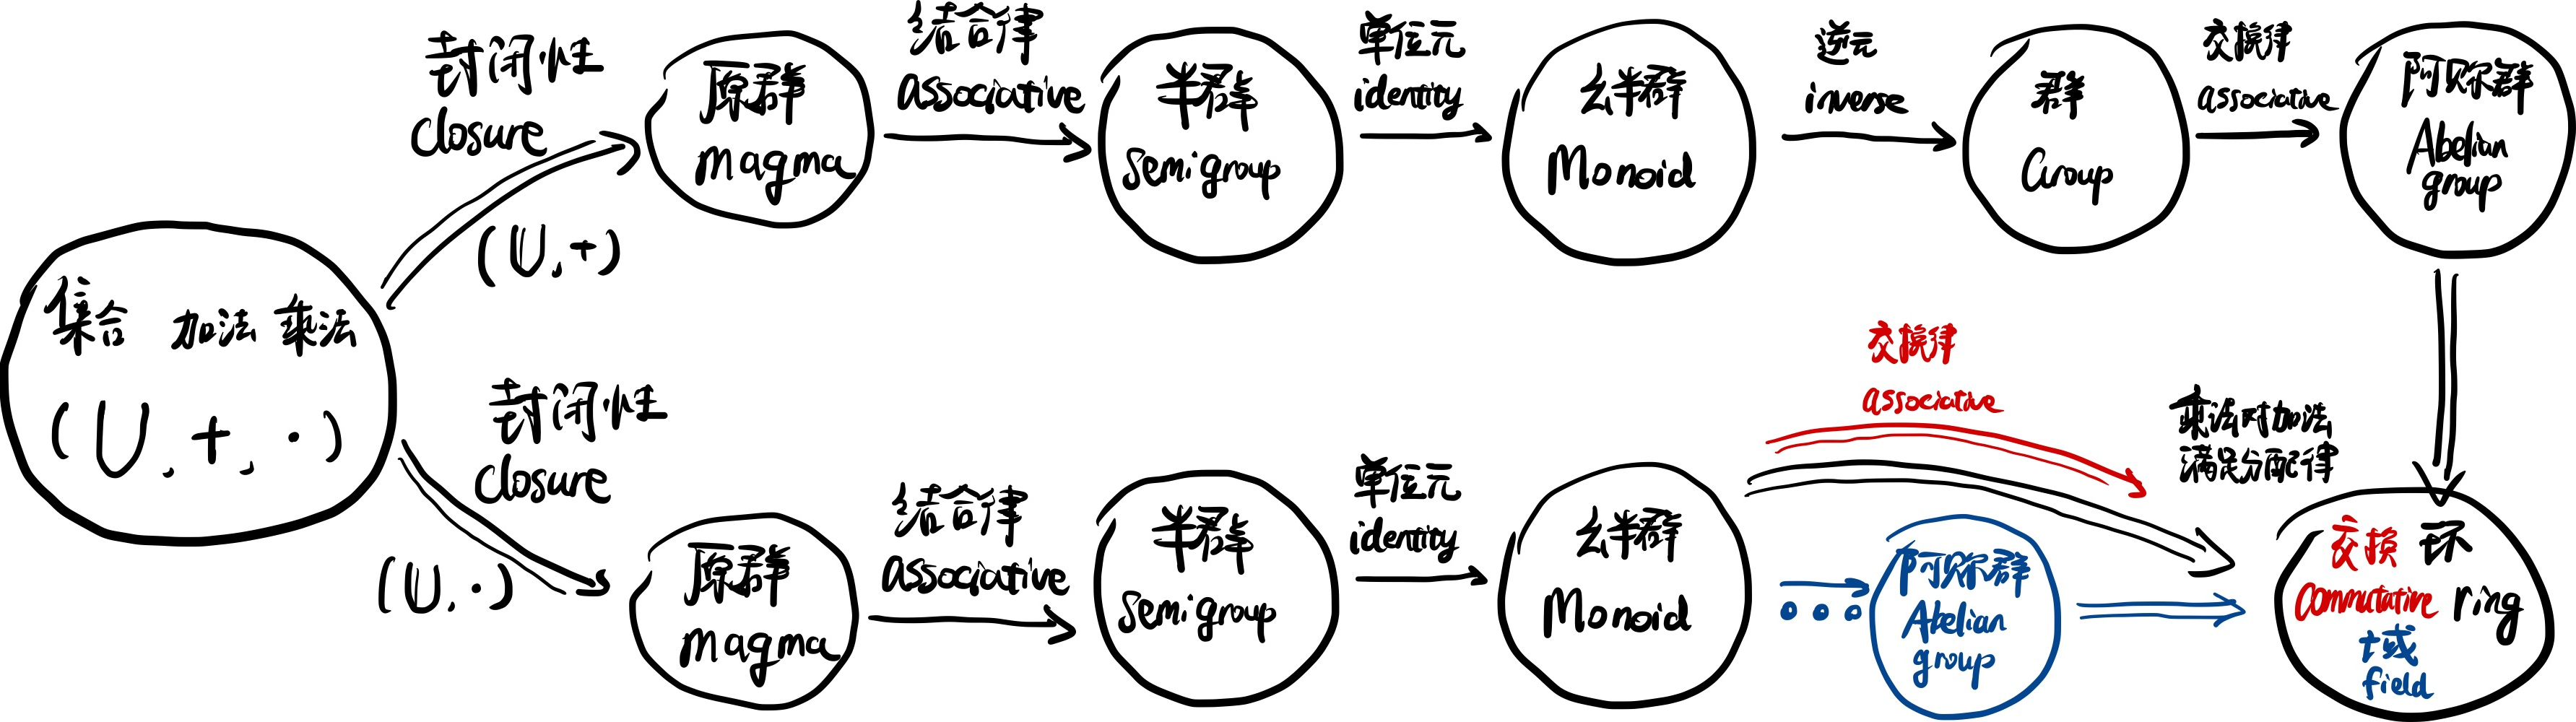
\includegraphics[width=0.9\textwidth]{img/image-20230328100716650.png}

\kaishu{\small 环, 交换环, 域的关系, 图改自知乎@SparkAndShine}
\end{tcolorbox}

\end{tcolorbox}
\begin{quote}
绕行之绕行 (detour of the detour).
\end{quote}

\hypertarget{ux4e8cux9879ux5f0fux5c55ux5f00-binomial-expansion}{%
\subsubsection{二项式展开 (binomial
expansion)}\label{ux4e8cux9879ux5f0fux5c55ux5f00-binomial-expansion}}

\textbf{二项式展开}指的是将类似 \((x+y)^n\) 的表达式展开的过程. 结论上有

\(\boxed{(x+y)^n=\sum_{r=0}^n\binom{n}{r}x^{n-r}y^r}.\)

这里 \(\binom{n}{r}=\frac{n!}{r!(n-r)!}\) 也记作 \(_nC_r\),
这个''C''是\textbf{组合} (combination) 的意思, 其中又有
\(n!=n\times(n-1)\times...\times3\times2\times1\).

\begin{quote}
上面第一次出现了求和符号 \(\sum\), 在此用一些例子说明,

\(\sum_{i=1}^{10}i=1+2+3+...+9+10;\)

\(\sum_{x=1}^{10}x^2=\left.x^2\right|_{x=1}+\left.x^2\right|_{x=2}+...+\left.x^2\right|_{x=10}=1^2+2^2+...+10^2.\)

即, 求和符号后的表达式, 依次代入求和符号下方的值,
符号下方的值加一\ldots, 直至代入求和符号上方的值, 最后将这些项求和.
\end{quote}

二项式展开的证明思路如下:

\textbf{从组合的思路出发}

\begin{itemize}
\item
  将 \((x+y)^n=\underbrace{(x+y)(x+y)...(x+y)}_{n}\) 展开,
  并将同类项合并, 易见可能出现的项的形式仅为 \(x^n=x^ny^0\),
  \(x^{n-1}y=x^{n-1}y^1\), \(x^{n-2}y^2\), \ldots{} \(x^2y^{n-2}\),
  \(xy^{n-1}=x^1y^{n-1}\), \(y^n=x^0y^n\).
\item
  合并后这些项的系数是合并前它们分别出现的次数,

  \begin{itemize}
  \tightlist
  \item
    \(x^n\) 相当于展开时每一个 \((x+y)\) 都选取 \(x\) 的情况,
    只有一种这样的情况, 即合并前 \(x^n\) 只可能出现 \(1\) 次,
    那么合并后它的系数便是 \(1\).
  \item
    \((x^{n-1}y^1)\) 相当于展开时每一个 \((x+y)\) 选取了 \((n-1)\) 个
    \(x\) 和 \(1\) 个 \(y\), 利用组合学的知识有
    \(n=\frac{n!}{1!(n-1)!}\) 种这样的情况, 即合并前 \((x^{n-1}y^1)\)
    出现 \(n\) 次, 那么合并后它的系数便是 \(n\).
  \end{itemize}

  \begin{quote}
  这个 \(n\) 可以这么看待, 选取的这个 \(y\) 可以出自这 \(n\) 项
  \((x+y)\) 中的任意一个, 于是便有 \(n\) 种可能.
  \end{quote}

  \begin{itemize}
  \tightlist
  \item
    \((x^{n-2}y^2)\) 相当于展开时每一个 \((x+y)\) 选取了 \((n-2)\) 个
    \(x\) 和 \(2\) 个 \(y\), 利用组合学的知识有
    \(\frac{n(n-1)}{2!}=\frac{n!}{1!(n-1)!}\) 种这样的情况, 即合并前
    \((x^{n-1}y^1)\) 出现 \(n\) 次, 那么合并后它的系数便是 \(n\).
  \end{itemize}

  \begin{quote}
  这个 \(\frac{n(n-1)}{2!}\) 可以这么看待, 选取的这两个 \(y\) 可以出自这
  \(n\) 项 \((x+y)\) 中的任意两个, 第一个 \(y\) 有 \(n\) 种选法,
  第二个因为第一个''占用''了一个 \((x+y)\), 因此它只有 \((n-1)\) 种选法,
  综上便有了 \(n(n-1)\); 然后两个 \(y\) 的顺序是无所谓的, 两个 \(y\)
  本身先后的排序会额外引入一个倍数 \(2\), 于是除掉.
  \end{quote}

  \begin{itemize}
  \tightlist
  \item
    \ldots{}
  \item
    \((x^{n-r}y^r)\) 相当于展开时每一个 \((x+y)\) 选取了 \((n-r)\) 个
    \(x\) 和 \(r\) 个 \(y\), 利用组合学的知识有
    \(\frac{n(n-1)...(n-r)}{(n-r)!}=\frac{n!/r!}{(n-r)!}=\frac{n!}{1!(n-1)!}=\binom{n}{r}\)
    种这样的情况, 即合并前 \((x^{n-1}y^1)\) 出现 \(\binom{n}{r}\) 次,
    那么合并后它的系数便是 \(\binom{n}{r}\).
  \end{itemize}

  \begin{quote}
  这个 \(\frac{n(n-1)...(n-r)}{(n-r)!}\) 可以这么看待, 选取的这 \(r\) 个
  \(y\) 可以出自这 \(n\) 项 \((x+y)\) 中的任意 \(r\) 个, 第一个 \(y\) 有
  \(n\) 种选法, 第二个因为第一个''占用''了一个 \((x+y)\), 因此它只有
  \((n-1)\) 种选法, 第三个于是只有 \((n-2)\) 种\ldots{} 综上便有了
  \(n(n-1)...(n-r)\); 然后 \(r\) 个 \(y\) 的顺序是无所谓的, \(r\) 个
  \(y\) 本身先后的排序, 第一个 \(y\) 顺序可能是 \(1\) 至 \(r\), 有 \(r\)
  种选择, 第二个只有 \((r-1)\)\ldots{} 于是会额外引入一个倍数
  \(r(r-1)...1=r!\), 于是除掉.
  \end{quote}
\item
  可见某一项 \((x^{n-r}y^r)\), 系数应为 \(\binom{n}{r}\), \(r=0\) 至
  \(r=n\) 的项都是允许的, 于是利用求和符号表示, 便有了最开始的结论.
\end{itemize}

这样的思路也可以推出杨辉三角 (Pascal's Triangle):

\begin{Shaded}
\begin{Highlighting}[]
    \FloatTok{1}
   \FloatTok{1}  \FloatTok{1}
  \FloatTok{1}  \FloatTok{2}  \FloatTok{1}
 \FloatTok{1}  \FloatTok{3}  \FloatTok{3}  \FloatTok{1}
\FloatTok{1}  \FloatTok{4}  \FloatTok{6}  \FloatTok{4}  \FloatTok{1}
\end{Highlighting}
\end{Shaded}

三角的左右两边由 \(1\) 填满, 中间的某个数字是左上和右上两个数字之和.
不难发现, 从第二行开始, 每一行的数字是都是二项式展开的系数.

上述的推导, 和类似【抛 \(n\) 次公平的硬币, 得到 \(r\) 次正面和 \((n-r)\)
次反面】的场景有着非常深的联系, 这里暂时不做展开.

\textbf{数学归纳法}

这个方法一般只能用于证明, 不能用于推导.

\begin{quote}
\textbf{数学归纳法} (proof by induction) 思路如下

\begin{enumerate}
\def\labelenumi{\arabic{enumi}.}
\tightlist
\item
  \textbf{归纳奠基} (base case), 证明第一个情况是对的;
\item
  归纳递推, 假设第 \(n\) 个情况正确, 以此推出第 \((n+1)\) 个情况正确,
  便有所有情况都成立.
\end{enumerate}

已知若情况n成立便有情况(n+1)也成立; 因为有情况1成立, 于是代入n=1,
便有情况2也成立; 现在知道情况2也成立了, 继续代入n=2,
便有情况3也成立\ldots{}
\end{quote}

思路已经给到, 具体证明留作练习. 一点提示是
\(\binom{r}{n+1}=\binom{r}{n}+\binom{r-1}{n}\).

\textbf{应用}

除了常规的 \(n\) 是整数的一些应用, 在保证展开的形式是\textbf{收敛}
(coverge) 的情况下 (即求和的形式不会趋向于正/负无穷),
二项式展开的负整数, 甚至分数形式也是成立的.

例如狭义相对论 (special relativity) 中, 随着物体运动速度变化,
物体的相对论性质量 (relativitic mass)\footnote{静止质量是物体静止时的质量,
  或者说某个观察者发现某物体处于静止状态下时这个物体的质量;
  相对论性质量则是物体相对观察者具有一定速度时, 观察者观察到的质量.}会变大,
它和静止质量 \(m_0\) 符合关系式

\(m=\frac{m_0}{\sqrt{1-v^2/c^2}}.\)

上式中 \(v\) 时速度, \(c\) 是光速. 根据幂运算的规律 (复习【002】),
上式可以改写成

\(m=m_0(1-v^2/c^2)^{-1/2}.\)

在估算例如速度在 \(0.01c\) 或更小时, 相对论性质量与静止质量之差,
直接计算 \((m-m_0)\) 通常看不出 \(m\) 与 \(m_0\) 的区别\footnote{计算机保存的并不是准确值,
  而是浮点数 (暂不展开), 可以暂且不太正确但道理就这么个道理地理解为:
  它保存的答案是一个写成科学计数法的数值, 并且位数有限,
  超过一定位数的部分就被切掉了;
  于是两个很接近的数字在计算机看来有可能是相等的, 进而计算不出差值.};
事实上, 我们可以利用二项式展开, 因为

\((1+x)^n=1+nx+\frac{n(n-1)}{2!}x^2+...,\)

代入 \(x=(v^2/c^2)\) 与 \(n=\frac{1}{2}\) 便有

\(m=m_0\left(1+(-1/2)\left(-\frac{v^2}{c^2}\right)+\frac{(-1/2)(-1/2-1)}{2!}\left(-\frac{v^2}{c^2}\right)^2\right)=m\left(1+\frac{v^2}{2c^2}+\frac{3}{8}\frac{v^4}{c^4}+...\right).\)

这个形式下, 相对论性质量与静止质量之差就很明显

\(m\left(\frac{v^2}{2c^2}+\frac{3}{8}\frac{v^4}{c^4}+...\right),\)

利用前几项便可以得到很好的近似.

绕行似乎要结束了, 之前的铺垫使得接下来的道路逐渐明朗\ldots{}

\hypertarget{ux81eaux7136ux5e38ux6570-natural-constant}{%
\subsubsection{自然常数 (natural
constant)}\label{ux81eaux7136ux5e38ux6570-natural-constant}}

通常自然常数会以下面两个例子引出:

\textbf{复利}

考虑一个奇怪的银行, 年利率是 \[100\%\], 也就是说, 存入 \[1\] 个货币,
到了年底便有

\[1\times(1+100\%)=2.\]

更奇怪的一点, 这家银行的单位时间利率不会因为存款周期改变, 也就是说, 存
\[0.5\] 年的利率是 \[0.5\times100\%=50\%\], 那么存半年连本带利取出,
再重新存入, 到了年底会怎么样?

\[1\times\left(1+\frac{100\%}{2}\right)^2=2.25.\]

年底的存款变多了! 那么如果存入更短的周期, 连本带息取出, 然后再存入,
重复这个操作到年末, 会怎么样呢? 考虑存取三次:

\[1\times\left(1+\frac{100\%}{3}\right)^3\approx2.37\].

可以发现年底存款变得更多了. 那如果这样存取的操作足够频繁,
到年底有可能赚取无限多的货币吗? 很可惜, 答案是否定的. 先上结论

\[\lim_{n\rightarrow\infty}\left(1+\frac{1}{n}\right)^n\approx2.71828.\]

虽然还没正式的介绍过''\textbf{极限}'' (limit), ``\textbf{收敛}''
(converge) 这些感念, 但是上式表的的意思是: 左边的 \[\lim\] 是取极限 -
limit - 的意思, 取当 \[n\] 趋向于无穷 (infinity) \[\infty\];
右边则是被取极限的形式, 在上式中, 右边的 \[n\] 便需要趋向于无穷.

计算上的话, 我们可以代入尽可能大的 \[n\],
大多数科学计算器是可以胜任这个估算的; 或者我们可以使用二项式展开
(参见【007】), 省略一些步骤, 不难得到

\[\lim_{n\rightarrow\infty}\left(1+\frac{1}{n}\right)^n=\frac{1}{0!}+\frac{1}{1!}+\frac{1}{2!}+...=\sum_{n=0}^\infty\frac{1}{n!}.\]

可以看到求和的形式, 加的项是逐渐变小的, 这个''变小''是足够快得,
使得整个求和是收敛的 (即有限的),
当然这个求和收敛的严格证明还算留到之后再细说.

既然复利的极限趋向于一个具体的数, 于是我们便规定这个数字叫自然常数:

\[\boxed{\lim_{n\rightarrow\infty}\left(1+\frac{1}{n}\right)^n\equiv\mathrm{e}=2.71828...}\]

\textbf{抽卡}

这也是一个经典的例子, 例如抽卡出货的概率是 \[\frac{1}{x}\],
那么不出货的概率便是 \[100\%-\frac{1}{x}\]; 日常我们会觉得,
比如抛硬币正面概率是 \[\frac{1}{2}\], 那么抛 \[2\]
次大概率上应该能出一个正面, 而事实上, 抛两次还是有挺大概率不出正面的,

从上图可见, 有 \[\frac{1}{4}\] 的概率抛出两次反面; 即, 反面的概率是
\[1-\frac{1}{2}=\frac{1}{2}\], 两次抛硬币互为独立事件,
因此两次都是反面的概率直接是这两个独立事件概率的乘积

\[\left (1-\frac{1}{2}\right)^2=0.25.\]

掷骰子也是一样, 我们总会觉得, 掷 \[6\] 次总''应该''出一个六点吧,
而事实上, 不出六点的概率是 \[1-\frac{1}{6}=\frac{5}{6}\], 于是掷 \[6\]
还是有可能不出六点的, 概率是

\[\left (1-\frac{1}{6}\right)^6\approx0.33.\]

回到抽卡的例子, 如果出货的概率非常非常小: 卡池里有茫茫多的 n 卡, r 卡,
\ldots{} , 只有那么一张 ssr, 要从几乎无限多的卡里抽出一张 ssr 来
(抽完要放回) , 但是相应的, 卡池越大抽卡次数也越多, 于是,
经历了无限次的抽卡后, 依旧有不出货的概率

\[\lim_{n\rightarrow\infty}\left (1-\frac{1}{n}\right)^n=0.367879...\]

同样可以利用二项式展开来估算

\[\lim_{n\rightarrow\infty}\left (1-\frac{1}{n}\right)^n=\frac{1}{0!}-\frac{1}{1!}+\frac{1}{2!}-\frac{1}{3!}...=\sum_{n=0}^\infty\frac{1^{n}}{n!}.\]

这个值事实上是 \[\frac{1}{\mathrm{e}}\]. 证明如下:

\[\begin{align}\left(\lim_{n\rightarrow\infty}\left (1-\frac{1}{n}\right)^n\right)^{-1}&=\lim_{n\rightarrow\infty}\left (1-\frac{1}{n}\right)^{-n}\\\text{(Let }m&=-n\text{ )}\\&=\lim_{n\rightarrow\infty}\left (1+\frac{1}{m}\right)^m\\&\equiv\mathrm{e,}\end{align}\]

可见
\[\boxed{\lim_{n\rightarrow\infty}\left (1-\frac{1}{n}\right)^n=\frac{1}{\mathrm{e}}}\].

\textbf{衰变}

这是笔者个人的一些经历, 本人高中阶段接触的物理教材是比较简单的那种,
于是衰变, 半衰期之类的讲得浅显, 大致有以下结论:

\begin{itemize}
\tightlist
\item
  单独一个原子衰变是一个完全随机的过程, 即我们不可知它具体的衰变时间;
  然而一堆同一种放射性原子, 经过一段时间, 未衰变的原子数量是之前的一半,
  这一段时间便叫做\textbf{半衰期} (half-life), 记作 \[t_{1/2}\];
\item
  没经过一个半衰期, 未衰变的原子数量是在这个半衰期前的数量的半; 即,
  假设某种元素的某个放射性同位素半衰期为一分钟, 一开始有 \[1000\]
  个这样的原子, 经过一分钟后, 大约还有 \[500\] 个没有衰变,
  再经过一分钟后, 还有大约 \[250\] 个没有衰变\ldots{}
\end{itemize}

于是, 用一个关于时间的函数来表示还未衰变的原子的数量便是

\[N(t)=N_0\times\left(\frac{1}{2}\right)^{t/t_{1/2}}.\]

但是用 \[\frac{1}{2}\] 作为底数看起来就很随意, 为什么不能是其他的比例呢?
应该也是可以的, 既然可以用变成原来 \[\frac{1}{3}\] , \[\frac{1}{4}\] ,
\ldots{} 的''三分之一衰期'', ``四分之一衰期'', \ldots{}
来表述某个时间还剩下多少未衰变的, 有没有更''自然''而不那么任意的底数呢?
于是便有\textbf{衰变常数} (decay constant)

\[\lambda:=\frac{\ln(2)}{T},\]

使得还未衰变的原子的数量可以表述为

\[N(t)=N_0\mathrm{e}^{-\lambda t}.\]

这其实是一个换底数的操作 (参见【002】), 不具体推导. 自然常数来了,
于是上面这个式子便''自然''起来了 (其实还没有). 当时稍稍初见这个公式时,
稍稍满意了一些, 但也不知道自然常数作为底数的深意; 直到很后来,
才知道当一个东西的变化率和它本身的大小成正比时 (比如这个衰变这个例子,
单位时间衰变的原子数量和当前未衰变的原子的数量是成正比的),
自然函数总会''自然地''出现.

\section{复数的指数形式}\label{009}

\begin{flushright}{\kaishu \textbf{虚}中有\textbf{实}者, 或山穷水尽处, 一折而豁然开朗. - 沈复
『浮生六记』 \\Lesson 5: 最短的捷径就是绕远路,
绕远路才是我的最短捷径.\footnote{\emph{ジョジョの奇妙な冒险 Part7
  スティ-ル・ボ-ル・ラン}.}}\end{flushright}

\begin{tcolorbox}[size=fbox, breakable, enhanced jigsaw, title={极坐标 (polar coordinate)}]

其实在\ref{005}\nameref{005}中已经借用了一点极坐标的概念, 这里再正式地介绍一遍.
在平面直角坐标系里, 一个点所在的位置具有两个自由度 (degree of freedom),
因此一般不多不少需要两个独立变量来锚定这个点, 通常我们会有一个点的
$x$-轴坐标和 $y$-轴坐标来表示这个点的位置 $(x,y)$. 当然,
我们也可以在建立坐标系后, 利用和原点的距离 $r$, 和一个方向,
例如【$x$-轴正方向】至【这个点和原点的连线】顺时针方向形成的夹角
$\theta$, 来表示一个点的位置 $(r,\theta)$.

\begin{tcolorbox}[size=fbox, breakable, enhanced jigsaw]
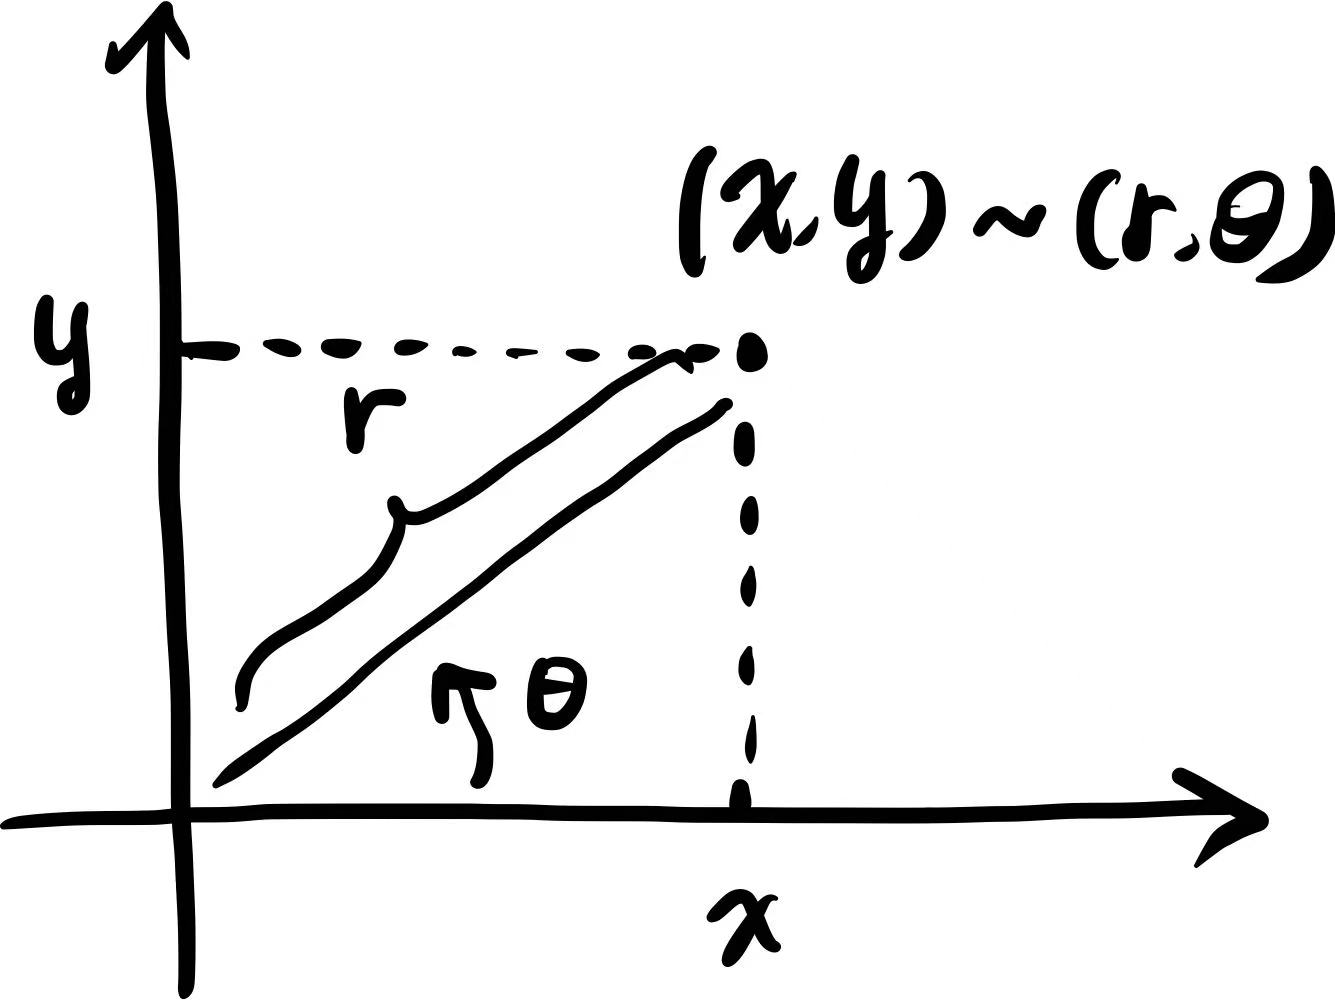
\includegraphics[width=0.5\textwidth]{img/image-20230418112700129.png}

\kaishu{\small 极坐标}
\end{tcolorbox}

不难看出, 存在以下的转换

$\begin{cases}x=r\cos\theta\\y=r\sin\theta\end{cases};\ \begin{cases}r=\sqrt{x^2+y^2}\\\theta=\arctan (y/x)\end{cases}.$

上式中 $\arctan$ 是 $\tan$ 的逆运算, 即
$\tan\theta=y/x\Rightarrow \theta=\arctan (y/x)$, 有时 $\arctan$
也记作 $\tan^{-1}$.

\end{tcolorbox}

\begin{tcolorbox}[size=fbox, breakable, enhanced jigsaw, title={复平面 (complex
plane)}]

考虑实数的时候, 有时我们会想象有一条数轴, 在\ref{001}\nameref{001}和\ref{002}\nameref{002}中,
我们将这条数轴添上了最初离散分布的整数,
然后又补上了似乎没有空隙的有理数, 最后才用全体实数彻底``填满''了.
在\ref{006}\nameref{006}中, 我们研究的对象再次扩展到了复数,
于是一条实轴似乎``放不下''这些复数的存在了, 我们便添加一条额外的,
与之前实数轴垂直的虚数轴, 如此一来便构成了一个复平面.

那么考虑一个复数 $(a+bi)$, 它的实部大小便是 $a$, 虚部大小便是 $b$,
仿照着实二维平面直角坐标系, 我们便可以在复平面上标出 $(a+bi)$
对应的一个点. 既然如此, 我们可以继续仿照着极坐标, 表示出至原点的距离,
以及 $x$-轴正方向到这个点和原点的连线顺时针方向形成的夹角,
这两个量在复平面中分别被称作\textbf{模} (modulus, 合理怀疑有音译成分)
和\textbf{辐角} (argument), 记作

$ | a+bi|=\sqrt{a^2+b^2},~\arg(a+bi)=\arctan (b/a).$

\begin{tcolorbox}[size=fbox, breakable, enhanced jigsaw]
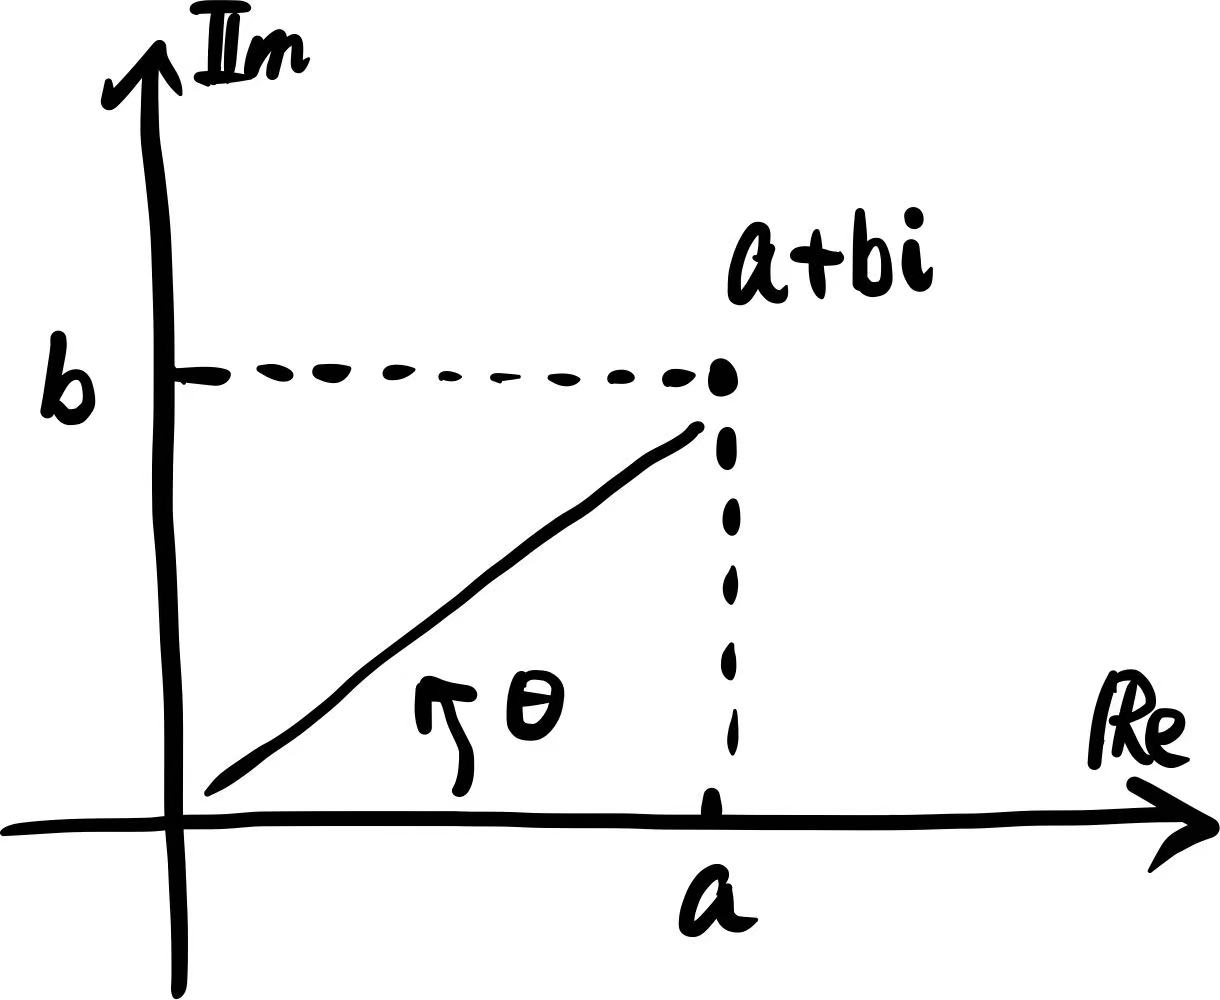
\includegraphics[width=0.5\textwidth]{img/image-20230418112740537.png}

\kaishu{\small 复平面}
\end{tcolorbox}

\begin{newquote}
像, 太像了.\footnote{\emph{让子弹飞}.}
\end{newquote}

若是把模和辐角分别记作 $r$ 和 $\theta$, 则这个复数 $(a+bi)$
便可以表示为

$(a+bi)=r\cos\theta+ir\sin\theta.$

\end{tcolorbox}

\begin{tcolorbox}[size=fbox, breakable, enhanced jigsaw, title={复数的指数形式}]

有那么一点跳脱, 怎么突然扯到指数了呢? 在\ref{002}\nameref{002}中,
其实我们只讨论过指数为有理数的情况, 当然指数是任意实数的情况, 例如
$\sqrt{2}$ , 我们也可以利用 $\sqrt{2}=1.414213...$ 去估算,
或者丢给一个科学计算器; 但是当指数是虚数或者复数时,
似乎情况就不大一样了\ldots 考虑自然常数为底数, 我们从自然常数的定义出发,
\ref{008}\nameref{008}中我们有

$\lim_{n\rightarrow\infty}\left(1+\frac{1}{n}\right)^n\equiv\mathrm{e}.$

不难推出, 对于任意实数 $x$, 有

$\lim_{n\rightarrow\infty}\left(1+\frac{x}{n}\right)^n=\mathrm{e}^x.$

把上面结论推广到虚数,

$\lim_{n\rightarrow\infty}\left(1+\frac{i}{n}\right)^n=\mathrm{e}^i.$

如果上式让您感到不适 (uncomfortable), 您大可用二项式展开 (参见\ref{007}\nameref{007})
来确认一下上述结果的正当性 (validity). 怎么理解这个 $\mathrm{e}^i$ 呢,
不妨来看看它的模和辐角.

在此之前, 我们还需要一些小\textbf{引理} (lemma \footnote{\textbf{公理/假定}
  (axiom/postulate): 默认为真无需证明的陈述. \textbf{定义} (definition):
  准确无歧义的对一个术语的描述. \textbf{定理} (theorem):
  证明为真的大结论. \textbf{引理} (lemma): 为了证明定理的小结论.
  \textbf{推论} (Corollary): 借助定理可简短地证明的结论.
  一本严格的数学书经常会出现前面这些令人畏惧的词,
  类似的还有\textbf{命题} (proposition), \textbf{推测/猜想}
  (conjecture), \textbf{断言} (claim)等等.}, 区别于 llama - 大羊驼,
好冷), 这里没有严谨证明, 仅提供一个思路:

\begin{tcolorbox}[size=fbox, breakable, enhanced jigsaw, title={引理1}]
$\boxed{|(a+bi)^n|=|a+bi|^n}$.
\end{tcolorbox}

\begin{newquote}
当 $n=2$ 时, $(a+bi)^2=a^2-b^2+2abi$. 于是

$\begin{aligned}|(a+bi)^2|=&\sqrt{(a^2-b^2)^2+(2ab)^2}\\=&\sqrt{(a^2+b^2)^2}\\=&\sqrt{(a^2+b^2)}^2\\=&|a+bi|^2.\end{aligned}$

用数学归纳法 (关于数学归纳法, 可以参见\ref{007}\nameref{007}中的一个实例)
便不难得出结论.
\end{newquote}

\begin{tcolorbox}[size=fbox, breakable, enhanced jigsaw, title={引理2}]
$\boxed{\arg((a+bi)^n)=n\cdot\arg(a+bi)}$.
\end{tcolorbox}

\begin{tcolorbox}[size=fbox, breakable, enhanced jigsaw, sidebyside]
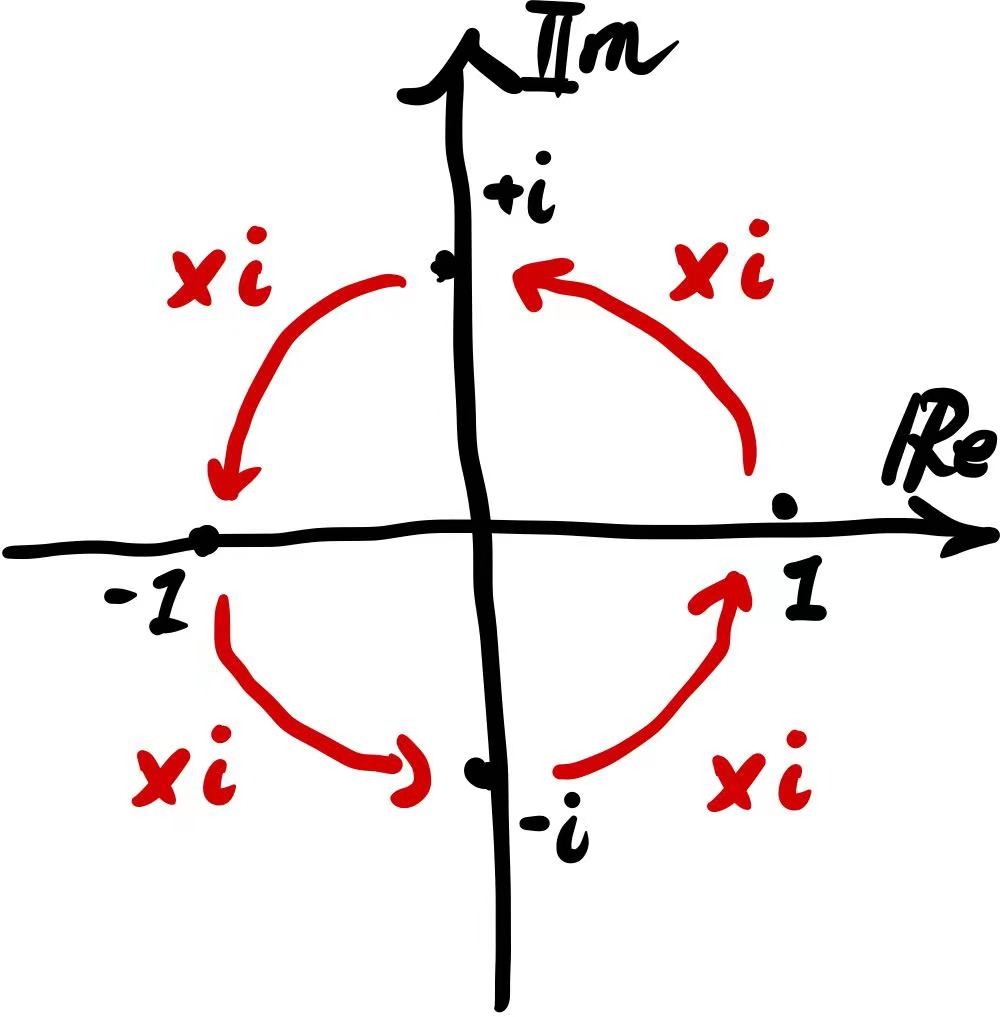
\includegraphics[width=0.9\textwidth]{img/image-20230418114331337.png}
\tcblower
\kaishu{\small 这里需要引入一个新的视角, 我们把复数看作一个``作用'',
将一个复数作用在某一个数 $z$ 上, 在复平面上事实上是将 $z$
对应的点关于原点旋转了. 考虑 $i\times1$, 即将 $i$ 作用到 $1$ 上,
得到了 $i$, 相当于逆时针旋转了 $90^\circ$; 继续作用 $i$, 得到了
$-1$, 相当于又逆时针旋转了 $90^\circ$\ldots{} 于是用 $i$ 作用
$n$ 次, 即作用了 $i^n$, 相当于将其作用对象, 关于原点, 旋转了 $i$
的辐角 $90^\circ$ $n$ 次, 便是旋转了 $n90^\circ$. ( $90^\circ$
用 $\pi/2$ 弧度表述其实会更好, 关于弧度可以参考\ref{005}\nameref{005},
下文若无额外说明, 角度皆用弧度制).

这个结论可以推广到其他任意复数, 便有了上述结论.}
\end{tcolorbox}

事实上, 利用辐角和模来表述一个复数, 上述两则引理可以总结成一条:

\begin{tcolorbox}[size=fbox, breakable, enhanced jigsaw, title={引理1+2}]
$\boxed{\left[r(\cos\theta+i\cos\theta)\right]^n=r^n(\cos n\theta+i\sin n\theta)}$.
\end{tcolorbox}

那么来看 $\mathrm{e}^i$ , 它的模

$\begin{aligned} |\mathrm{e}^i|=&\left|\lim_{n\rightarrow\infty}\left(1+\frac{i}{n}\right)^n\right|\\ =&\lim_{n\rightarrow\infty}\left|\left(1+\frac{i}{n}\right)^n\right|\\ =&\lim_{n\rightarrow\infty}\sqrt{1+\frac{1}{n^2}}^n\\ =&\lim_{n\rightarrow\infty}\left(1+\frac{1}{n^2}\right)^{n/2}\\ =&\lim_{n\rightarrow\infty}\left[\left(1+\frac{1}{n^2}\right)^{n^2}\right]^{1/2n}=\lim_{n\rightarrow\infty}\mathrm{e}^{1/2n}=1. \end{aligned}$

上式第二行到第三行利用了引理1, 最后一行先是利用了自然常数的定义, 然后当
$n\rightarrow\infty$ 便有 $1/2n\rightarrow0$, 于是
$\mathrm{e}^0=1$. 再来看辐角

$\begin{aligned} \arg(\mathrm{e}^i)=&\lim_{n\rightarrow\infty}n\arg\left(1+\frac{i}{n}\right)\\ =&\lim_{n\rightarrow\infty}n\arctan\frac{1}{n}=\lim_{n\rightarrow\infty}n\frac{1}{n}=1.\\ \end{aligned}$

上式先是利用了引理2, 然后当 $n\rightarrow\infty$ 时
$1/n\rightarrow0$, 然后在这个极限下 (啊, 还是,
极限我们晚点再稍严格地讨论) 有
$\arctan\frac{1}{n}\rightarrow\frac{1}{n}$.

\begin{newquote}
当然也可以用\textbf{小角度近似} (small angle approximation) 来理解
(注意, 是理解不是证明) 这个过程. 小角度近似即, 使用弧度制时, 当
$\theta\ll1$, 有 $\theta\approx\sin\theta\approx\tan\theta$.
\end{newquote}

这样利用模和辐角, 我们有

$\mathrm{e}^i=\cos1+i\sin1$.

所以 $\mathrm{e}^i$ 在复平面上对应一个距离原点 $1$, 与原点连线和
$x$-轴夹角是 $1$ 的点, 或者说 $\mathrm{e}^i$ 是一个实部是
$\cos1$, 虚部是 $\sin1$ 的复数. 不难推广到 $|\mathrm{e}^{ib}|=1$,
$\arg(\mathrm{e}^{ib})=b$, 进而

$\mathrm{e}^{ib}=\cos b+i\sin b$.

早一些地结论
$\lim_{n\rightarrow\infty}\left(1+\frac{i}{n}\right)^n=\mathrm{e}^i$
其实可以推广到任意复数 $(a+ib)$, 即
$\lim_{n\rightarrow\infty}\left(1+\frac{a+ib}{n}\right)^n=\mathrm{e}^{a+ib}=\mathrm{e}^{a}\mathrm{e}^{ib}$,
那么

$\boxed{\mathrm{e}^{a+ib}=\mathrm{e}^a(\cos b+i\sin b)}$\footnote{a+ib
  取 iπ 便可以得到著名的欧拉公式, 确实非常美丽, 虚实正负在此交汇,
  圆周率和自然常数也藏于其中.}.

\end{tcolorbox}
\begin{quote}
(有名、无名) 此两者同出而异名, 同谓之玄, 玄之又玄, 众妙之门.
\end{quote}

前面介绍三角函数 (【005】) 的时候, 跳过了一些比较重要的\textbf{恒等式}
(identities), 比如: \[\cos (a\pm b)=?\], \[\sin (a\pm  b)=?\]

事实上这些恒等式可以从纯几何出发去推导,
或者也可以用所谓诱导公式\footnote{有一说''诱导''是谬译, induction
  在数学中更常译作''归纳''.} (induction formula, 即三角函数的周期性),
再或者, 在【009】中我们发现三角函数和指数函数有着联系,
我们也可以利用这层关系.

\hypertarget{ux4e09ux89d2ux51fdux6570ux7684ux6307ux6570ux5f62ux5f0f}{%
\subsubsection{\texorpdfstring{\{三角函数的指数形式
\label{title}\}}{\{三角函数的指数形式 \}}}\label{ux4e09ux89d2ux51fdux6570ux7684ux6307ux6570ux5f62ux5f0f}}

先前我们有,

\[\mathrm{e}^{i\theta}=\cos \theta+i\sin \theta\],

代入 \[\theta:=-\theta\]\footnote{这里仿照了编程里常用的记法,
  在很多语言中程序猿可能会写 a = a + 1, 这行指令并不表示 a 等于 a + 1,
  而表示将 a 这个变量赋值它原先的值加一, 例如若起先有 a = 1,
  那么在执行了 a = a + 1 后, a 变为了 a = 1 + 1 = 2.}, 便有
\[\mathrm{e}^{-i\theta}=\cos (-\theta)+i\sin (-\theta)\],
利用三角函数的周期性可得,

\[\mathrm{e}^{-i\theta}=\cos \theta-i\sin \theta\],

将前两式相加便可消去 \[\sin\theta\] 项, 相减便可消去 \[\cos\theta\] 项,
化简便可得

\[\boxed{\cos\theta=\frac{\mathrm{e}^{i\theta}+\mathrm{e}^{-i\theta}}{2},\ \sin\theta=\frac{\mathrm{e}^{i\theta}-\mathrm{e}^{-i\theta}}{2i}}\].

\hypertarget{ux5229ux7528ux63a8ux5bfcux4e09ux89d2ux51fdux6570ux6052ux7b49ux5f0f}{%
\subsubsection{\texorpdfstring{利用\ref{title}推导三角函数恒等式}{利用推导三角函数恒等式}}\label{ux5229ux7528ux63a8ux5bfcux4e09ux89d2ux51fdux6570ux6052ux7b49ux5f0f}}

以 \[\cos (a+b)\] 为例:

\[\begin{aligned}&\cos(a+b)\\
=&\frac{\mathrm{e}^{i(a+b)}+\mathrm{e}^{-i(a+b)}}{2}\\
=&\frac{2\mathrm{e}^{i(a+b)}+2\mathrm{e}^{-i(a+b)}}{4}\\
=&\frac{\mathrm{e}^{i(a+b)}\bbox[silver]{+\mathrm{e}^{i(a-b)}+\mathrm{e}^{i(-a+b)}}+\mathrm{e}^{-i(a-b)}}{4}+\frac{\mathrm{e}^{i(a+b)}\bbox[silver]{-\mathrm{e}^{i(a-b)}-\mathrm{e}^{i(-a+b)}}+\mathrm{e}^{-i(a-b)}}{4}\\
=&\frac{\mathrm{e}^{ia}+\mathrm{e}^{-ia}}{2}\frac{\mathrm{e}^{ib}+\mathrm{e}^{-ib}}{2}-\frac{\mathrm{e}^{ia}-\mathrm{e}^{-ia}}{2i}\frac{\mathrm{e}^{ib}-\mathrm{e}^{-ib}}{2i}\\
=&\cos a\cos b-\sin a\sin b.\end{aligned}\]

类似的, 可以得到

\[\boxed{\cos(a\pm b)=\cos a\cos b\mp \sin a \sin b,\\
\sin(a\pm b)=\sin a\cos b\pm \cos a\sin b.}\]

另外还有常用的二倍角公式, 可令上式中的 \[a=b\] 得到,

\[\boxed{\sin2a=2\sin a\cos a,\\
\cos2a=\cos^2a-\sin^2a=2\cos^2a-1=1-2\sin^2a,}\]

第二个等式利用了 \[\sin^2\theta+\cos^2\theta=1\]. 再还有有时会有半角,
可以用 \[\cos\] 的二倍角公式推导, 例如, 求 \[\cos\] 的半角公式可以令
\[\cos\] 的二倍角公式中的 \[a:=a/2\],

\[\cos a=2\cos^2(a/2)-1\],

整理可得

\[\boxed{\cos\frac{a}{2}=\pm\sqrt{\frac{1+\cos a}{2}}}.\]

类似的

\[\boxed{\sin\frac{a}{2}=\pm\sqrt{\frac{1-\cos a}{2}}}.\]

\[\tan\] 相关的公式则可以利用 \[\tan=\sin/\cos\] 求得.

\chapter{微积分 (calculus)}
\begin{flushright}{\kaishu 天\ 工\ 开\ 物\ !\\「Made in Heaven!」要开始加速了\footnote{ジョジョの奇妙な冒险 Part 6
  スト-ンオ-シャン}}\end{flushright}

\section{极限和连续性}\label{011}

跳过一些内容: 集合 (set), 点集拓扑 (point set topology), 数列与级数
(sequence and series); 如果您希望习得更加严谨的数学语言, 那么可以移步
Walter Rudin - \emph{Principles of Mathematical Analysis} (俗称 baby
Rudin\footnote{Baby = 数学分析原理 \emph{Principles of Mathematical
  Analysis}; Papa/Big = 实分析与复分析 \emph{Real and Complex Analysis};
  Grandpa = 泛函分析 \emph{Functional Analysis}; 好好地学严格的数学,
  逃不掉这三本分析, 这个系列也就看个乐子.}).

\subsection{极限 (limit)}

\begin{tcolorbox}[size=fbox, breakable, enhanced jigsaw, title={定义}]
当 $x$ 趋向于 $p$ 时, $x\rightarrow p$ , $f(x)$
趋向于 $q$, $f(x)\rightarrow q$ , 记作
$\lim_{x\rightarrow p}f(x)=q.$

用 $\epsilon - \delta$ 语言 (出现了!) 来说,
$\lim_{x\rightarrow p}f(x)=q$ 便是: 对于任意的 $\epsilon>0$ , 存在
$\delta>0$ 使得【若 $0<|x-p|<\delta$, 便有 $|f(x)-q|<\epsilon$
】\footnote{其实这里的定义还是很不严谨, 比如没有说明定义域和值域.
  为了省笔墨下文都默认取值范围在合适的区间内.}.

\end{tcolorbox}

为什么要用 $\epsilon - \delta$ 语言? 原本的``趋向于''其实很不严格,
什么叫趋向于呢, 于是 $\epsilon - \delta$ 语言如是说道:

\begin{itemize}

\item
  我先任意选定一个 $\epsilon$,
\item
  然后我要试着找到一个 $\delta$,
\item
  使得 $x$ 与 $p$ 足够接近时 - 有多接近呢? 它们差的绝对值
  (或者说``距离'', 不过这边还没定义距离, 233) 小于 $\delta$ - 便有
  $f(x)$ 与 $q$ 足够接近 - 多近呢? 他们差的绝对值小于 $\epsilon$.
\item
  若对于任意小的 $\epsilon$, 总能找到一个这样的 $\delta$,
  那么便可以放心地说, 确有$\lim_{x\rightarrow p}f(x)=q$.
\end{itemize}

\begin{tcolorbox}[size=fbox, breakable, enhanced jigsaw]
  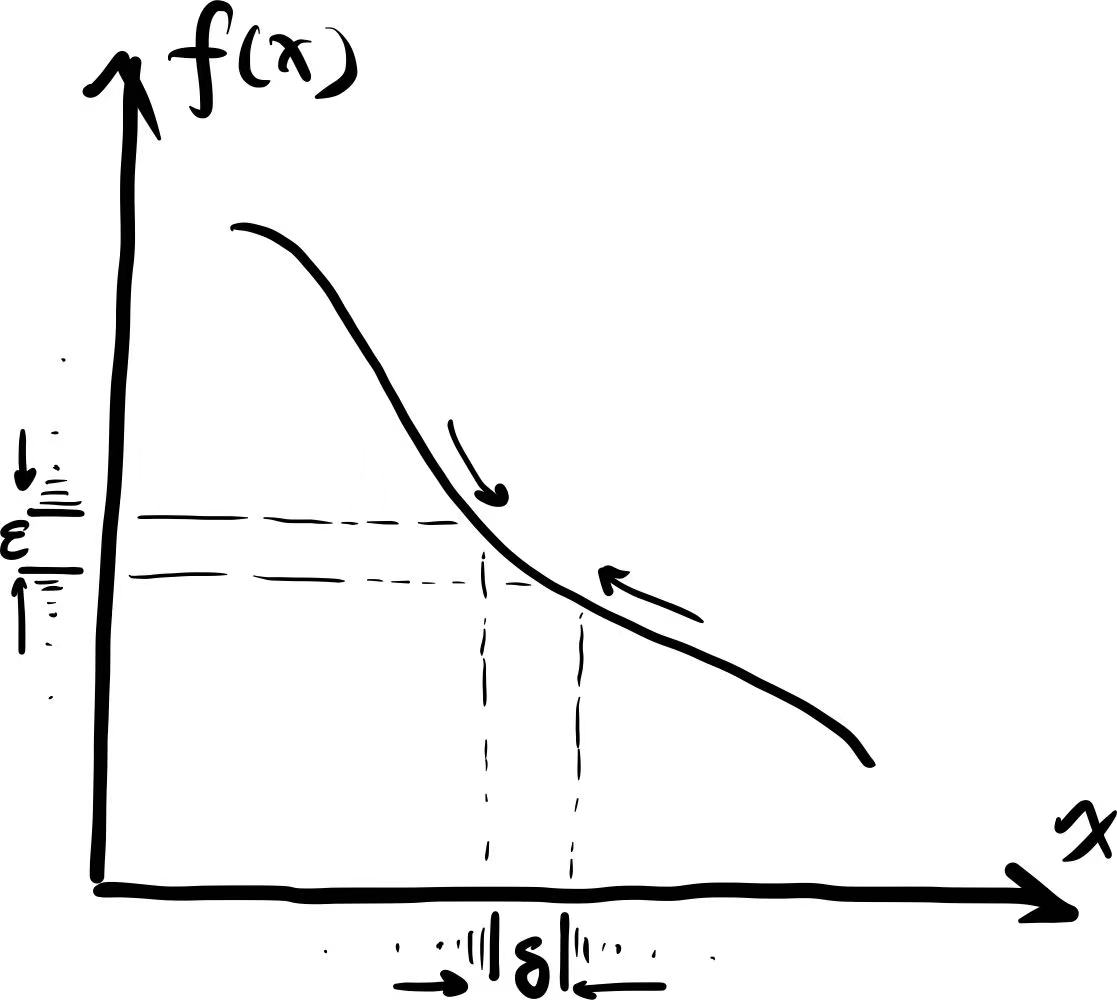
\includegraphics[width=0.45\textwidth]{img/image-20230503152041842.png}
\end{tcolorbox}

\begin{newquote}
\textbf{例子}: 一个平凡的情况 (a trivial case), $f(x)=ax$, 证明
$\lim_{x\rightarrow 1}f(x)=a$.

\textbf{思路} (草稿纸上或者脑子里的部分): 对于任意 $\epsilon>0$
我们需要找到 $\delta>0$, 满足当 $0<|x-1|<\delta$ 时,
$|f(x)-a|<\epsilon$ 成立.

\begin{itemize}
\item
  $|f(x)-a|=|ax-a|=a|x-1|$
\item
  令上式小于 $\epsilon$, 发现有 $|x-1|<\epsilon/a$
\item
  令 $\delta=\epsilon/a$ , 即可出锅食用 (bushi).
\end{itemize}

\textbf{证明} (写下来的正式的书面的部分): 对任意 $\epsilon>0$ , 令
$\delta=\epsilon/a$, 则当 $0<|x-1|<\delta$ 时, 有

\begin{itemize}

\item
  $|f(x)-a|=|ax-a|=a|x-1|<a\delta<\epsilon$.
\item
  于是根据极限的定义, $\lim_{x\rightarrow 1}f(x)=a$
\end{itemize}

Q.E.D\footnote{Quod erat demonstrandum - 这被证明了.}

\textbf{吐槽}: 鄙人学分析的时候学得就很不到位,
写证明的时候常常向同学``借鉴'', 时常觉得, 证明本身并不难写,
难得是想到并``构造''出一些证明需要的东西, 就如在上面的例子中构造一个
$\delta=\epsilon/a$;
殊不知``借鉴''的那些作业其实只有上面例子中【证明】的部分,
而【思路】部分被写在草稿纸上丢掉了.
这种狡猾如雪地上的狐狸一般用尾巴扫去自己的踪迹的行为\ldots{}
于是有这样的说法:

一位菲尔兹得主告诉我, 顶级的数学家们会秘密地像物理学家一样思考,
等他们得到证明的一个大框架之后, 他们再用 epsilon 和 delta
的语言把证明过程包装起来.
\end{newquote}

\begin{itemize}

\item
  若 $f(x)$ 在 $x\rightarrow p$ 处存在极限,
  这个极限是\textbf{唯一}的 (unique).
\end{itemize}

考虑 $\lim_{x\rightarrow p}f(x)=a$, $\lim_{x\rightarrow p}g(x)=b$,
极限还存在以下规律 (啊, 美好的线性) :

\begin{itemize}

\item
  $\lim_{x\rightarrow p}(f\pm g)(x)=a\pm b$;
\item
  $\lim_{x\rightarrow p}(fg)(x)=ab$;
\item
  $\lim_{x\rightarrow p}\frac{f}{g}(x)=\frac{a}{b}$, 若 $b\neq 0$.
\end{itemize}

\begin{newquote}
回收一个坑. 【\ref{002}\nameref{002}】中提到过 $\mathrm{0}^0$ 是未被定义的问题,
一种解释便是, 若希望用极限来定义它的取值, 那么应该从
$\lim_{x\rightarrow0}x^0$ 出发, 得到 $1$, 还是应该从
$\lim_{x\rightarrow0}0^x$ 出发, 得到 $0$?
\end{newquote}


\subsection{连续性 (continuity)}

\textbf{定义}: 对于一函数 $f(x)$, 对于任意的 $\epsilon>0$ , 存在
$\delta>0$ 使得【对于某个特定的 $x_0$, 若有 $x$ 满足
$|x-x_0|<\delta$, 便有 $|f(x)-f(x_0)|<\epsilon$】, 那么我们便可以说,
$f(x)$ 在 $x_0$ 处连续.

\begin{itemize}

\item
  若 $f(x)$ 和 $g(x)$ 连续, 那么 $f(g(x))$ 也连续.
\item
  若 $f(x)$ 和 $g(x)$ 连续, 那么 $(f\pm g)(x)$, $fg(x)$,
  $\frac{f}{g}(x)$ 都连续, 最后一条要求 $g(x)$ 对于任意 $x$ 不为
  $0$.
\end{itemize}

从连续性出发, 可以得到以下几个定理, 图像上非常直观, 这边暂时忽略严格证明.

\begin{tcolorbox}[size=fbox, breakable, enhanced jigsaw, title={极值定理 (extreme value theorem)}]

\begin{tcolorbox}[size=fbox, breakable, enhanced jigsaw, sidebyside]
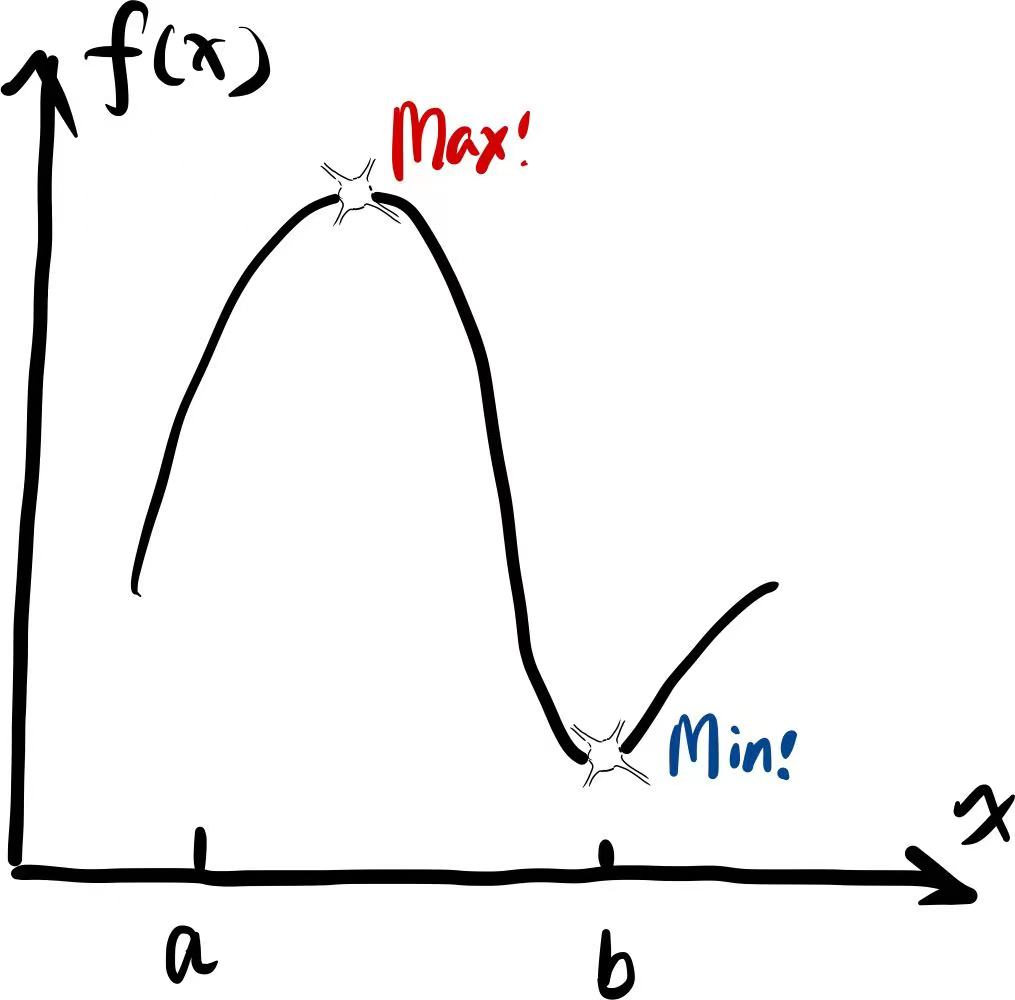
\includegraphics[width=0.9\textwidth]{img/image-20230503152124313.png}
\tcblower
\kaishu{\small 若函数 $f(x)$ 在区间 $[a,b]$ 连续, 则 $f(x)$ 必然在区间 $[a,b]$
存在最大值和最小值.}
\end{tcolorbox}

\end{tcolorbox}

\begin{tcolorbox}[size=fbox, breakable, enhanced jigsaw, title={介值定理 (intermediate value theorem)}]

\begin{tcolorbox}[size=fbox, breakable, enhanced jigsaw, sidebyside]
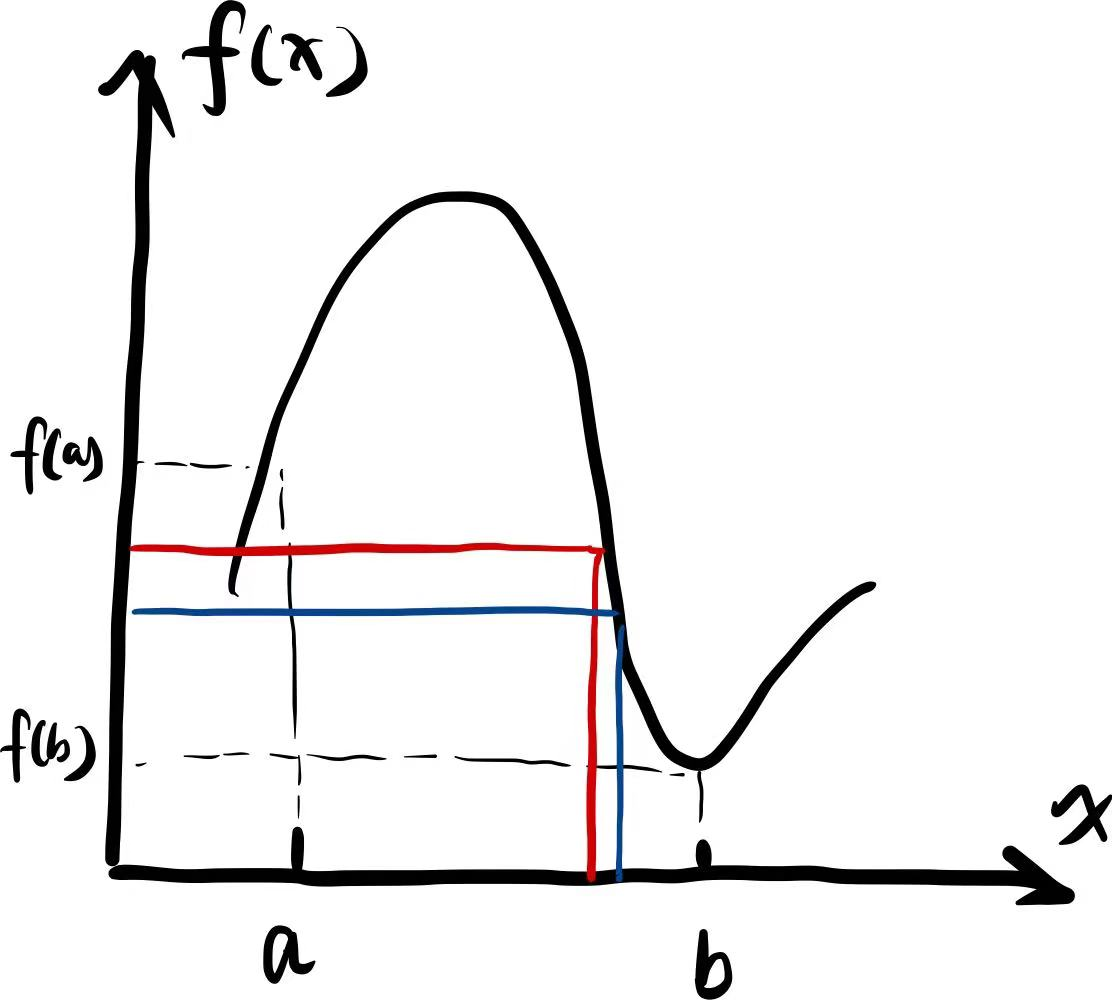
\includegraphics[width=0.9\textwidth]{img/image-20230503152147199.png}
\tcblower
\kaishu{\small 若函数 $f(x)$ 在区间 $[a,b]$ 连续, 且有 $f(a)<C<f(b)$ 或
$f(a)>C>f(b)$, 那么总是存在 $c\in(a,b)$ 或者说 $a\le c\le b$ 使得
$f(c)=C$.}
\end{tcolorbox}

\end{tcolorbox}

\begin{tcolorbox}[size=fbox, breakable, enhanced jigsaw, title={零点定理 (zero theorem)}]

\begin{tcolorbox}[size=fbox, breakable, enhanced jigsaw, sidebyside]
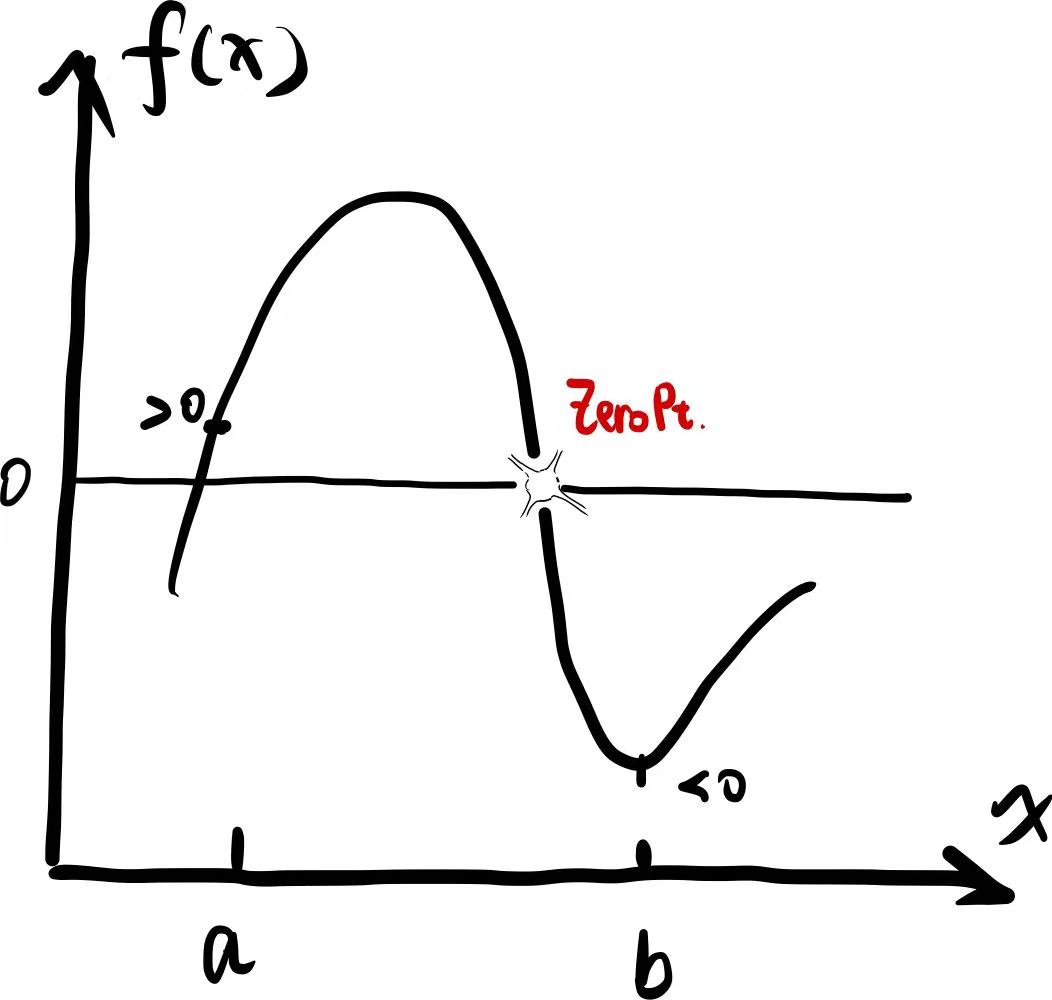
\includegraphics[width=0.9\textwidth]{img/image-20230503152707849.png}
\tcblower
\kaishu{\small 若函数 $f(x)$ 在区间 $[a,b]$ 连续, 且$f(a)f(b)<0$, 则存在
$c\in(a,b)$ 使得 $f(c)=0$.}
\end{tcolorbox}

\end{tcolorbox}

\hypertarget{ux5bfcux6570-derivative}{%
\subsubsection{导数 (derivative)}\label{ux5bfcux6570-derivative}}

初中阶段常有求二次函数切线的题目,
利用初中知识求切线的表达式往往过程冗长, 事实上, \textbf{微积分}
(calculus) 会大大简化这个过程. 微积分, 如其名所示, 分为\textbf{微分}
(differentiation) 和\textbf{积分 }(integration).

在这里我们姑且先用经典的角度来了解微积分. \textbf{微分} (differential)
可以不严谨的理解为\textbf{无穷小量} (infinitesimal),
这是一些物理教材中更常见的表述, 例如某函数 \(y=f(x)\),
它的一个有限的变化通常记作 \(\Delta y\), 这个小三角念作''delta'',
在很多场景下表示变化, 而一个无穷小量的变化便记作 \(\mathrm{d}y\).
任何实数都比无穷小量大, 就像无穷大 \(\infty\) 大于任何实数{[}\^{}1{]}.

另有一个非常类似的概念叫做\textbf{导数}, 导数可以理解为函数的变化率.
考虑某函数 \(y=f(x)\) 在一个很小但是有限的一个定义域区间 \([a,b]\),
有自变量的变化为 \(\Delta x=b-a\), 函数值的变化为
\(\Delta y= f(b)-f(a)\), 于是在此区间内''平均''变化率是

\(\frac{\Delta y}{\Delta x}=\frac{f(b)-f(a)}{b-a}.\)

若是希望得到 \(x=a\) 处的变化率, 我们令 \(h:=b-a\), 直觉上应该是
\(\lim_{h\rightarrow0}[f(a+h)-f(a)]/h\), 这便是函数 \(f(x)\) 在 \(x=a\)
处的变化率, 或 \(f(x)\) 在 \(x=a\) 处的导数. 推广到任意位置 \(x\), 遂有:

\textbf{定义}: 函数 \(f(x)\) 的导(函)数\footnote{取某个特定的点 x=x\_0,
  得到的导数是一个具体数值, 便叫它导数; 若不将 x 锚定到一个特定的值,
  导数便依旧是一个含 x 的函数, 便叫它导函数. 下文不再区分. 类似的,
  后文再出现的微分, 导数和无穷小量也不再严格区分.}为

\(\lim_{h\rightarrow0}\frac{f(x+h)-f(x)}{h}.\)

很多数学教材会这么标记导数

\(\boxed{f'(x)=\lim_{h\rightarrow0}\frac{f(x+h)-f(x)}{h}}.\)

物理教材更偏好

\(\frac{\mathrm{d}y}{\mathrm{d}x}=\lim_{h\rightarrow0}\frac{f(x+h)-f(x)}{h}.\)

\begin{quote}
举一个例子, 若一个物体非匀速运动, 将速度 \(v\) 表示为一个关于时间 \(t\)
的函数 \(v(t)\), 那么便有加速度 (acceleration) 即速度的变化率:
\(a(t)=v'(t)=\frac{\mathrm{d}v}{\mathrm{d}t}\).

另: 很多时候, 物理中, 关于时间的求导还有一个标记,
\(\dot{f}\equiv \frac{\mathrm{d}f}{\mathrm{d}t}\)\footnote{很多人经常吐槽物理中标记的不统一.
  个人当然也觉得, 如果有一套统一的标记, 信息的沟通自然会便利不少;
  但是学习的过程中, 既然标记不统一已经客观存在, 与其花时间吐槽,
  不如去抓住本质, 不要拘泥于标记, 而去理解标记背后的含义.}.
\end{quote}

类似 \(\frac{\mathrm{d}y}{\mathrm{d}x}\) 这样记法的好处是,
``变化率''这个概念被表现得很直观, 若有
\(\frac{\mathrm{d}y}{\mathrm{d}x}=y'(x)\), 我们可以将它改写为
\(\mathrm{d}y=y'(x)\mathrm{d}x\), 虽然''两边同乘 \(\mathrm{d}x\)''
这个说法非常不正确的, 但是从''变化率''的角度出发的确可以这么理解.

\textbf{定理}: 若 \(f(x)\) 在 \(x=c\) 存在导数 (我们也可以说, 它在
\(x=c\) 处可以被求导), 那么它在 \(x=c\) 处连续.

(不严格的) \textbf{证明}: 不使用 \(\epsilon - \delta\) 语言的话,
只需证明 \(\lim_{x\rightarrow c}f(x)=f(c)\) 即可. 于是, 对于有限的
\(h\), \(f(c+h)=f(c)+f(c+h)-f(c)=f(c)+\frac{f(c+h)-f(c)}{h}\cdot h\),
取极限 \(h\rightarrow0\) 有
\(\lim_{h\rightarrow0}f(c+h)=\lim_{h\rightarrow0}f(c)+\lim_{h\rightarrow0}\frac{f(c+h)-f(c)}{h}\cdot h=f(c)+f'(c)\cdot 0\),
第一个等号利用了极限的线性, 第二个等号则需要导数存在,
于是便有存在导数隐含 (imply) 连续.

若有函数 \(f(x)\) 和 \(g(x)\), 导数的一些性质:

\begin{itemize}
\tightlist
\item
  \((af+bg)'(x)=af'(x)+bg'(x)\), 这里 \(a\) 和 \(b\) 是常数;
\item
  \((fg)'(x)=f'(x)g(x)+f(x)g'(x)\);
\item
  \(\left(\frac{f}{g}\right)'(x)=\frac{f'(x)g(x)-f(x)g'(x)}{g^2(x)}\),
  若 \(g(x)\neq 0\).
\end{itemize}

第一条性质可以由极限的线性而来; 第二条和第三条可以分别令
\(h(x)=f(x)g(x)\) 和 \(h(x)=\frac{f(x)}{g(x)}\), 然后将 \(h(x)\)
代入导数的定义.

下面是一个非常 trivial 的例子,

\begin{quote}
\textbf{例子}: \(y(x)=x^2\), 求 \(y'(x)\). 利用定义:
\(\begin{aligned}y'(x)=&\lim_{h\rightarrow0}\frac{(x+h)^2-x^2}{h}\\=&\lim_{h\rightarrow0}\frac{x^2+h^2+2xh-x^2}{h}\\=&\lim_{h\rightarrow0}(2x+h^2)\\=&2x.\end{aligned}\)
\end{quote}

不难将结果推广为

\(\boxed{\frac{\mathrm{d}}{\mathrm{d}x}x^n=nx^{n-1}}.\)

{[}\^{} 1{]}: 【007】中有提到过''浮点数'', 例如一个有理数 a,
它不会被以分数的形式记录, 而是记录其小数形式并精确到某一位,
那么第一个非零位数低于这一位的数字 b, 它对于 a 来说在计算机数值上看来,
便等效于无穷小量. 在 MATLAB 中, 给定一个实数 a, 利用函数 eps(), eps(a)
便会输出对于 a 来说的''无穷小量''.

\hypertarget{ux5e38ux89c1ux51fdux6570ux7684ux5bfcux6570}{%
\subsubsection{常见函数的导数}\label{ux5e38ux89c1ux51fdux6570ux7684ux5bfcux6570}}

\textbf{指数函数}

从指数函数开始, 首先考虑自然常数作为底数的情况, 代入导数的定义: \$\$

\begin{aligned}
\frac{\mathrm{d}}{\mathrm{d}x}(\mathrm{e}^x)=&\lim_{h\rightarrow0}\frac{\mathrm{e}^{x+h}-\mathrm{e}^x}{h}\\

=&\lim_{h\rightarrow0}\mathrm{e}^x\left(\frac{\mathrm{e}^h-1}{h}\right)\\
\\
&\text{令 }n:=1/h\\
\\
=&\lim_{n\rightarrow\infty}\mathrm{e}^x\left(\frac{\mathrm{e}^{1/n}-1}{1/n}\right)\\
\\
&\text{根据定义 }\mathrm{e}\equiv\lim_{n\rightarrow\infty}\left(1+\frac{1}{n}\right)^n\\
\\
=&\lim_{n\rightarrow\infty}\mathrm{e}^x\left(\frac{{\left(\left(1+1/n\right)^n\right)}^{1/n}-1}{1/n}\right)\\

=&\lim_{n\rightarrow\infty}\mathrm{e}^x\left(\frac{1+1/n-1}{1/n}\right)\\

=&\mathrm{e}^x.
\end{aligned}

\$\$

于是 \[
\boxed{\frac{\mathrm{d}}{\mathrm{d}x}\mathrm{e}^x=\mathrm{e}^x}.
\]

对于其他的底数, 例如 \(a^x\), 我们需要一些额外的知识了:

\textbf{链式法则 chain rule}

结论上有: \[
\boxed{\frac{\mathrm{d}y}{\mathrm{d}x}=\frac{\mathrm{d}y}{\mathrm{d}u}\frac{\mathrm{d}u}{\mathrm{d}x}}.
\]

\begin{quote}
即原先有一个函数 \(y=h(x)\), 将它改写为一个符合函数 \(y=f(g(x))\), 并令
\(u:=g(x)\).

不严格的直觉上的证明:

\(\Delta u=g(x+\Delta x)-g(x)\), \(\Delta y=f(u+\Delta u)-f(u)\). 于是
\(\frac{\Delta y}{\Delta x}=\frac{\Delta y}{\Delta u}\frac{\Delta u}{\Delta x}\).
再取 \(\Delta x\rightarrow0\) 的极限, 若 \(g(x)\) 是连续的, 在
\(\Delta x\rightarrow0\) 时便有 \(\Delta u\rightarrow 0\),
于是便得到了上述结论.
\end{quote}

现在我们再来看 \(a^x\), 我们可以先利用【002】的知识换个底数,
\(a^x=\mathrm{e}^{\ln(a)x}\), 再利用链式法则, 令 \(y:=\mathrm{e}^u\)
\(u:=\ln{(a)}x\), 于是 \$\$

\begin{aligned}
\frac{\mathrm{d}}{\mathrm{d}x}(a^x)=&\frac{\mathrm{d}y}{\mathrm{d}u}\frac{\mathrm{d}u}{\mathrm{d}x}\\

=&(\mathrm{e}^u)(\ln{a})\\

=&(\ln{a})\mathrm{e}^{\ln{a}}=(\ln{a})a^x.
\end{aligned}

\[
更加通常 (generalize) 一点, 我们可以有
\]
\boxed{\frac{\mathrm{d}}{\mathrm{d}x}a^{u(x)}=(\ln{a})a^u\frac{\mathrm{d}u}{\mathrm{d}x}}.
\$\$ \textbf{三角函数}

先考虑 \(\sin\), \$\$

\begin{aligned}
\frac{\mathrm{d}}{\mathrm{d}x}(\sin(x))=&\lim_{h\rightarrow0}\frac{\sin(x+h)-\sin(x)}{h}\\
\\
& \text{ 参见【010】, }\sin(a\pm b)=\sin a\cos b\pm \cos a\sin b\\
\\
=&\lim_{h\rightarrow0}\frac{\sin(x)\cos(h)+\cos(x)\sin(h)-\sin(x)}{h}\\

=&\lim_{h\rightarrow0}\left(\frac{\sin(x)(\cos(h)-1)}{h}+\frac{\cos(x)\sin(h)}{h}\right),
\end{aligned}

\$\$

到这一步似乎就不很直观了, 若是直接取 \(h=0\), 则有 \(\cos(h)-1=0\) 和
\(\sin(h)=0\), 两项的分子分母都同时为零了, 类似这种出现了
\(\frac{0}{0}\) 或者 \(\frac{\infty}{\infty}\) 的情况称为不定式/未定型
(indeterminate forms), 后面我们会看到将有一种更便 (简单) 捷 (粗暴)
的方式来解决这样的问题 (剧透: 洛必达法则 - L'Hôpital's rule),
目前我们先老老实实地来解决. 对于上面的形式, 我们可以用几何方法入手:

如上图所示, 考虑一个单位圆, 三角形 \(OAB\), 扇形 \(OAD\), 和三角形
\(OCD\) 的面积关系是 \(\sin(\theta)/2<\theta/2<\tan(\theta)/2\);
将每个式子都除以 \(\sin(\theta)/2\), 有
\(1<\theta/\sin(\theta)<1/\cos(\theta)\); 再取倒数, 得到
\(1>\sin(\theta)/\theta>\cos\theta\).
这个结论至少在第一象限应该是成立的, 于是当我们取 \(\theta=0\) 时,
我们发现不等式的最右边也是 \(1\) 了, 直觉上, 中间一项既要比 \(1\) 小,
又要比 \(1\) 大, 那么它只能是等于 \(1\) 了. 这个朴素的想法被叫做
``三明治定理'' (Sandwich Theorem, 也叫夹逼定理\ldots).

这样一来, 便有当 \(h\rightarrow0\), \(\sin(h)/h\rightarrow 1\),
另一项的话, 也不难利用三角函数的恒等式变形: \[
\begin{aligned}
&\frac{\cos(h)-1}{h}\\
\\
&\text{参见【010】}\cos2a=1-2\sin^2a\\
\\
=&-\frac{2\sin^2(h/2)}{h}\\
\\
&\text{令 }\theta:=h/2
\\
=&-\frac{\sin(\theta)}{\theta}\cdot\sin(\theta),
\end{aligned}
\]

于是当 \(h\rightarrow0\), \(\theta\rightarrow0\), \[
\begin{aligned}
&\frac{\cos(h)-1}{h}\\
=&-\frac{\sin(\theta)}{\theta}\cdot\sin(\theta)\\
=&-(1)\cdot(0)\\=&0.
\end{aligned}
\] 综上, \[
\boxed{\frac{\mathrm{d}}{\mathrm{d}x}(\sin(x))=\cos(x)}.
\] 类似的, 不难推出 \[
\boxed{\frac{\mathrm{d}}{\mathrm{d}x}(\cos(x))=-\sin(x)}.
\]

\textbf{逆函数和导数}

有的时候我们会有一个函数的反函数 (关于反函数可以参见【004】),
而不是这个函数本身, 求这个函数的导数时, instead of
先求反函数的反函数得到原函数, 我们可以利用反函数本身来求这个导数, \[
\begin{aligned}
f(f^{-1}(x))=&x\\
\text{(对两边求导)}\\
\frac{\mathrm{d}}{\mathrm{d}x}f(f^{-1}(x))=&1\\
\text{(利用链式法则)}\\
f'(f^{-1}(x))\cdot\frac{\mathrm{d}}{\mathrm{d}x}f^{-1}(x)=&1\\
\text{(rearrange)}\\
\boxed{\frac{\mathrm{d}}{\mathrm{d}x}f^{-1}(x)=\frac{1}{f'(f^{-1}(x))}}.
\end{aligned}
\]

\textbf{对数函数}

这样一来, 因为我们已经知道对于指数函数有
\[\frac{\mathrm{d}}{\mathrm{d}x}\mathrm{e}^x=\mathrm{e}^x\],
便可借助上式得到对数函数的导数了, \[
\begin{aligned}
\frac{\mathrm{d}}{\mathrm{d}x}\ln(x)=&\frac{\mathrm{d}}{\mathrm{d}x}\exp^{-1}(x)\\
&\text{(利用上式结论, 令 }f^{-1}(x):=\ln(x),\\
&\text{ 于是 }f(x)=\exp(x), f'(x)=\exp(x)\text{ )}\\
=&\frac{1}{\exp(\ln(x))}\\
=&\frac{1}{x},
\end{aligned}
\] 因此 \[
\boxed{\frac{\mathrm{d}}{\mathrm{d}x}\ln(x)=\frac{1}{x}}.
\] 当然, 也可以直接利用换元, 令 \[y:=\ln(x)\], 于是有 \[\exp(y)=x\],
于是 \[
\begin{aligned}
\frac{\mathrm{d}}{\mathrm{d}x}\exp(y)=&\frac{\mathrm{d}}{\mathrm{d}x}(x)\\
\exp(y)\frac{\mathrm{d}y}{\mathrm{d}x}=&1\\
\frac{\mathrm{d}y}{\mathrm{d}x}=&\frac{1}{\exp(y)}=\frac{1}{\exp(\ln(x))}=\frac{1}{x}.
\end{aligned}
\] 不难得出, 更通常而言, 有 \[
\boxed{\frac{\mathrm{d}}{\mathrm{d}x}\log_au=\frac{1}{\ln(a)\cdot u}\frac{\mathrm{d}u}{\mathrm{d}x}}.
\] \textbf{反三角函数}

利用逆函数和导数的关系, 类似的, 不难推出, \[
\begin{aligned}
\frac{\mathrm{d}}{\mathrm{d}x}\sin^{-1}(x)=&\frac{1}{\cos(\sin^{-1}(x))}\\
=&\frac{1}{\sqrt{1-\sin^2(\sin^{-1}(x))}}\\
=&\frac{1}{\sqrt{1-x^2}}.
\end{aligned}
\] 更通常的, \[
\boxed{\sin^{-1}(u)=\frac{1}{\sqrt{1-u^2}}\frac{\mathrm{d}u}{\mathrm{d}x}}.
\] 和前面类似的, 也可以利用换元得到同样的结果, 考虑一个单位圆, 有
\[\theta=\sin^{-1}(y)\], 于是 \[\sin(\theta)=y\], 对两边同时求导, 有
\[\cos(\theta)\frac{\mathrm{d}\theta}{\mathrm{d}y}=1\], 继而有 \[
\begin{aligned}
\frac{\mathrm{d}\theta}{\mathrm{d}y}=&\frac{1}{\cos(\theta)}\\
&\text{(在单位圆里有 }\cos(\theta)= x\text{)}\\
=&\frac{1}{x}\\
=&\frac{1}{\sqrt{1-y^2}}.
\end{aligned}
\] 这样的方法其实有利用隐函数 \[x^2+y^2=1\],
之后我们还会看到隐函数的导数和微分方程有一些联系.

另一个常用的反三角函数的导数 \[
\boxed{\frac{\mathrm{d}}{\mathrm{d}x}\tan^{-1}(u)=\frac{1}{1+u^2}\frac{\mathrm{d}u}{\mathrm{d}x}}.
\] 推导过程可以留作练习.

\section{导数的应用}\label{015}

先前我们有利用导数求函数的切线过, 这里我们继续来看导数还有那些应用.

\begin{tcolorbox}[size=fbox, breakable, enhanced jigsaw, title={一次导和极值}]

导数可以视作切线的斜率, 所以可以利用导数的正负判断函数的增减性,
当导数大于$0$ 时, 函数是递增的, 当导数小于$0$ 时, 函数是递减的.

若函数 $f(x)$ 有局域的最大或最小值 (统称极值) 在 $x=c$ 处, 且
$f'(x)$ 在 $x=c$ 处是被定义的, 那么 $f'(c)=0$.

\begin{newquote}
不太严谨的证明:

\begin{itemize}

\item
  考虑 $x=c$ 附近足够小的邻域 (neighborhood) , 使得在此领域内
  $f'(x)$ 是连续的;
\item
  因为 $f(c)$ 是极值: 则在 $x=c$ 的一侧, 有 $f'(x)>0$
  (切线斜率为正, 函数递增); 另一侧, 有 $f'(x)<0$ (切线斜率为负,
  函数递减);
\item
  利用零点定理 (参见【\ref{011}\nameref{011}】) , 这个领域中必然有一点使得 $f'(x)=0$,
  利用极限可得这个点恰好在 $x=c$ 上.
\end{itemize}
\end{newquote}

\begin{newquote}
一个 trivial 的例子:

利用上述性质, 我们来找一下二次函数的顶点.

若有函数 $f(x)=y=ax^2+bx+c$, 于是 $f'(x)=2ax+b$, 当 $f'(x)=0$,
$2ax+b=0$, 于是 $x=\frac{b}{2a}$. 将 $x=\frac{b}{2a}$ 代入原函数,
得到 $y=f\left(\frac{b}{2a}\right)=\frac{4ac-b^2}{4a}$.

这个结论和配方得到的结论是一致的
$y=a\left(x-\frac{b}{2a}\right)^2+\frac{4ac-b^2}{4a}$.
\end{newquote}

对于更复杂的函数, 也可以用同样的思路来求极值

\begin{itemize}

\item
  先对函数求导;
\item
  令导数为 $0$, 求得导数为 $0$ 处的自变量取值;
\item
  将求得的自变量取值代入原函数, 得到函数极值.
\end{itemize}

\end{tcolorbox}

\begin{tcolorbox}[size=fbox, breakable, enhanced jigsaw, title={二次导和凹凸性}]

我们可以对导数继续求导, 二次导可以这么记: $f''(x)\equiv \frac{\mathrm{d}^2f}{\mathrm{d}x^2}\equiv \frac{\mathrm{d}}{\mathrm{d}x}\frac{\mathrm{d}f}{\mathrm{d}x}$. 考虑一个有二次导的的函数\footnote{有的学科里会称为 $C^2$ 连续.}:

\begin{itemize}

\item
  若 $f''(x)>0$, 则函数是上凹的 (concave up);
\item
  若 $f''(x)<0$, 则函数是下凹的 (concave down);
\end{itemize}

\begin{tcolorbox}[size=fbox, breakable, enhanced jigsaw, sidebyside]
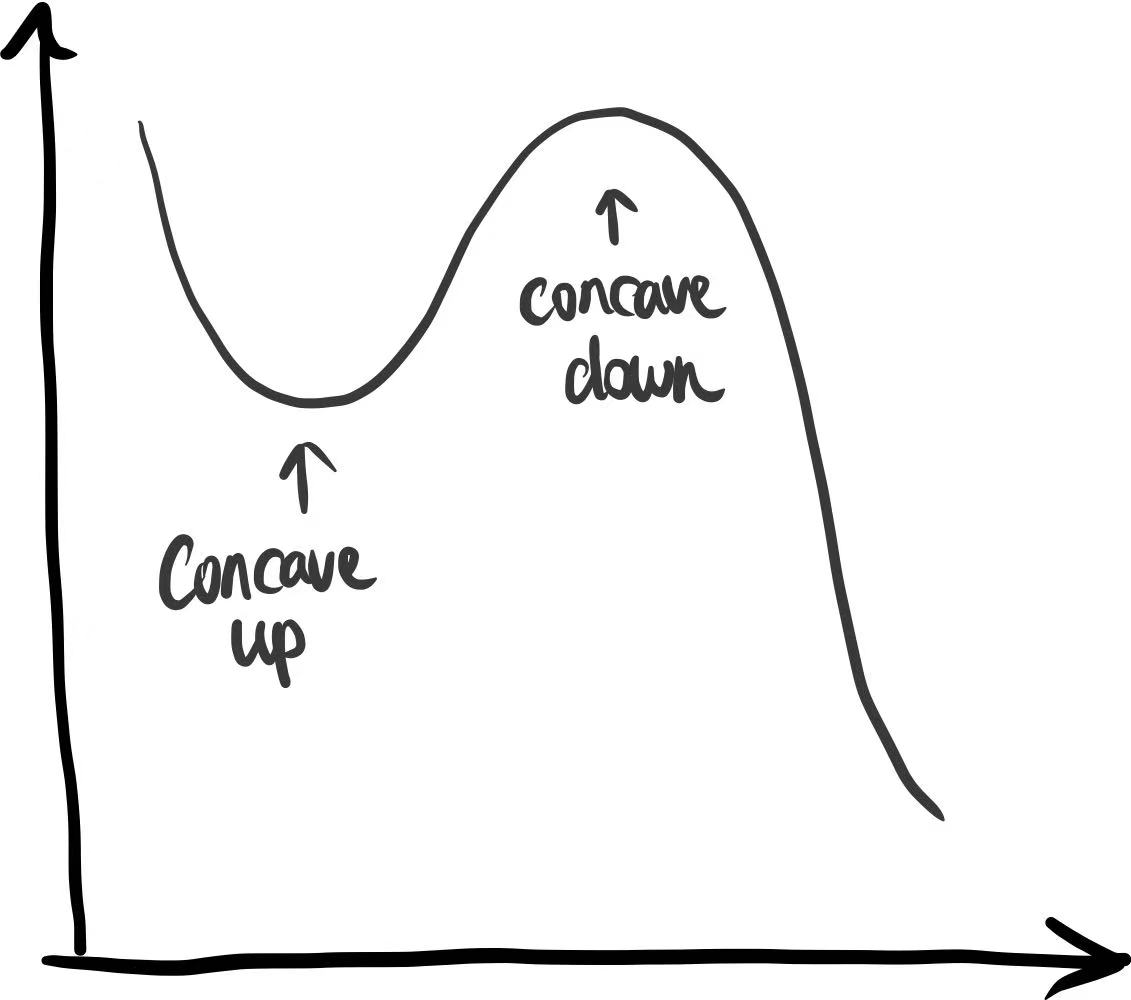
\includegraphics[width=0.9\textwidth]{img/image-20230614143547029.png}
\tcblower
\kaishu{\small }
\end{tcolorbox}

对于二次函数而言, 上凹下凹便对应着开口向上和开口向下.

函数的凹凸性发生变化的点我们称之为拐点 (point of inflection),
有时也称为驻点. 在拐点处, $f''(x)=0$ 或不存在 (例如趋向于无穷).

\end{tcolorbox}

\subsection{洛必达法则 (L'Hôpital's
rule)}

在【\ref{013}\nameref{013}】中, 在求三角函数的导数时, 我们遇到了极限是不定式/未定型的情况,
先前我们利用几何法绕开了这种情况, 现在我们来看怎么和这种情况刚正面.

\begin{tcolorbox}[size=fbox, breakable, enhanced jigsaw, title={罗尔中值定理 (Rolle's theorem)}]



\begin{tcolorbox}[size=fbox, breakable, enhanced jigsaw, sidebyside]
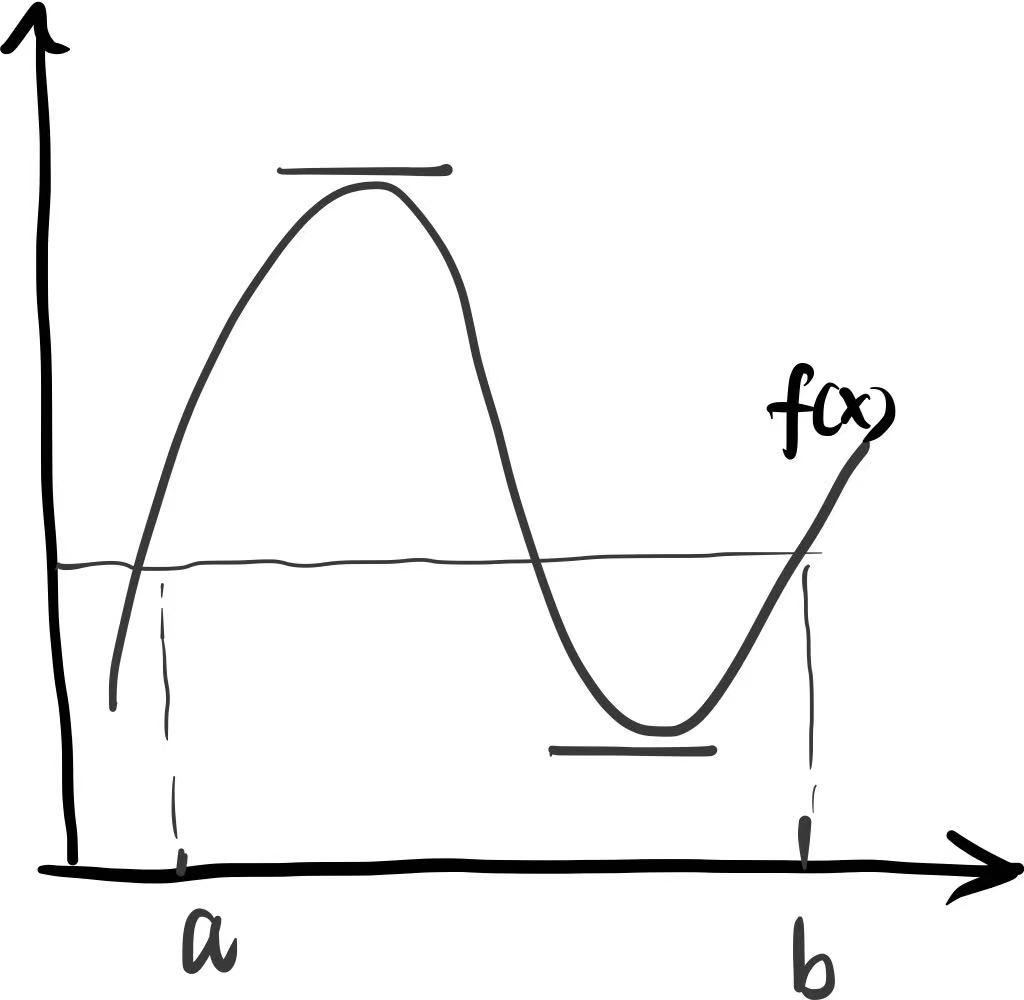
\includegraphics[width=0.9\textwidth]{img/image-20230615082313476.png}
\tcblower
\kaishu{\small 若 $f(x)$ 在区间 $[a,b]$ 连续, 且在区间 $(a,b)$ 可微或存在导数,
如果 $f(a)=f(b)$, 则至少存在一个点 $x=c$ 使得 $f'(c)=0$.\\很直观, 一定存在一个斜率正负值变化的地方, 处非是一个 trivial 的情况,
即函数为一个常数, 那么斜率处处为 $0$.}
\end{tcolorbox}

\begin{newquote}
证明思路:

极值定理 (参见【\ref{011}\nameref{011}】) 告诉我们区间 $[a,b]$ 存在极值, 前面我们还发现,
极值处的导数为 $0$.
\end{newquote}

\end{tcolorbox}

\begin{tcolorbox}[size=fbox, breakable, enhanced jigsaw, title={拉格朗日中值定理 (Lagrange mean value theorem)}]



\begin{tcolorbox}[size=fbox, breakable, enhanced jigsaw, sidebyside]
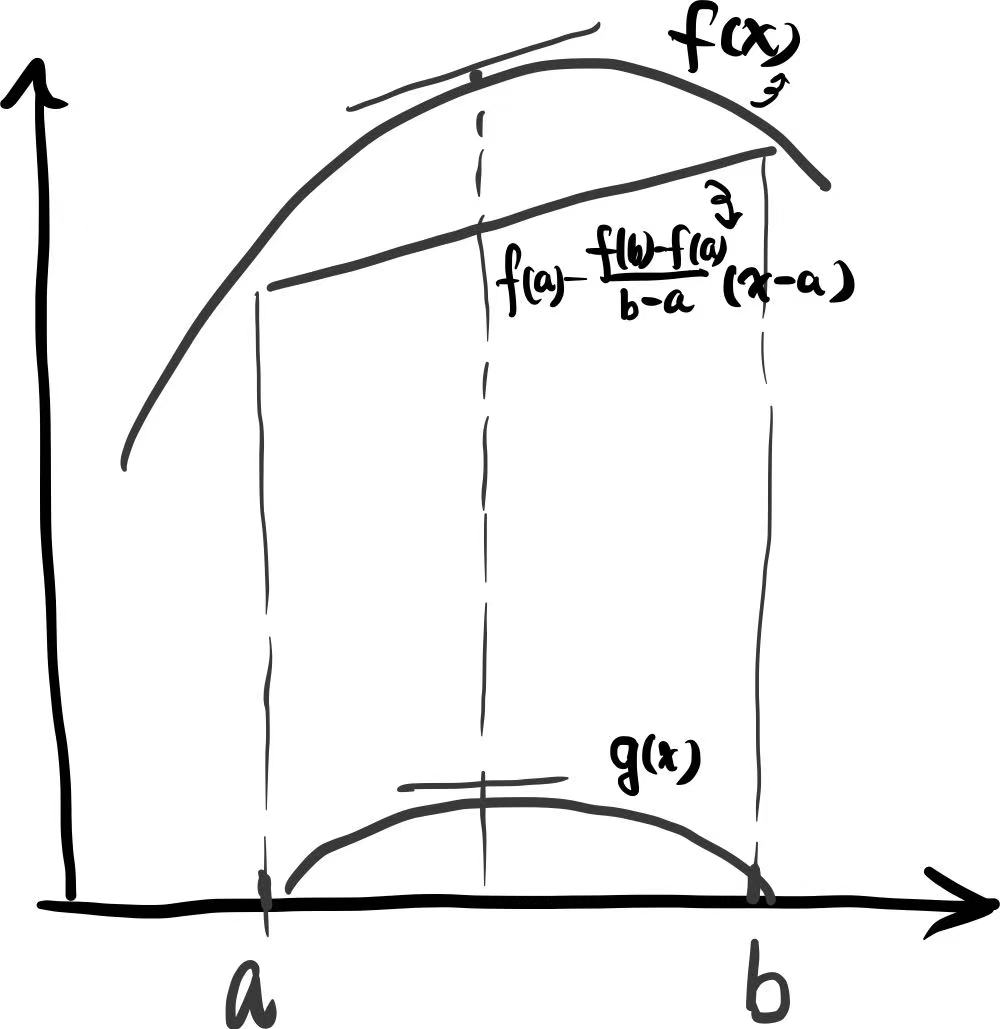
\includegraphics[width=0.9\textwidth]{img/image-20230615082602908.png}
\tcblower
\kaishu{\small 若 $f(x)$ 在区间 $[a,b]$ 连续, 且在区间 $(a,b)$ 可微或存在导数,
则至少存在一个点 $x=c$ 使得 $f'(c)=\frac{f(b)-f(a)}{b-a}$.}
\end{tcolorbox}

\begin{newquote}
证明思路:

这是罗尔中值定理''加强版'', 可以从罗尔中值定理出发去证明.
最后的结论可以理解为,
这个区间存在一个点使得【函数的斜率】和【函数在这个区间两个端点连线的斜率】一致.
因为斜率和连线的斜率一致, 也就是说, 【原函数】减去【两端点连线的函数】,
所得到的新的函数在这个点斜率是 $0$.

\begin{itemize}

\item
  综上, 构造这样一个函数 (最难的一步, 关于这一点的吐槽参见【\ref{011}\nameref{011}】,
  因为最后的), 令 $g(x):=f(x)-f(a)-\frac{f(b)-f(a)}{b-a}(x-a)$.
\item
  易见这样一来 $g(a)=g(b)=0$, 利用罗尔中值定理, 可得存在一点 $x=c$
  使得 $g'(c)=0$.
\item
  $g'(x)=f'(x)-\frac{f(b)-f(a)}{b-a}$, 这里要注意 $f(a)$ 和 $f(b)$
  已经将 $x=a$ 和 $x=b$ 分别代入了原函数, 是一个具体数值了;
\item
  于是 $g'(c)=f'(c)-\frac{f(b)-f(a)}{b-a}=0$, 证毕.
\end{itemize}
\end{newquote}

\end{tcolorbox}

\begin{tcolorbox}[size=fbox, breakable, enhanced jigsaw, title={柯西中值定理 (Cauchy's mean value theorem)}]



\begin{tcolorbox}[size=fbox, breakable, enhanced jigsaw, sidebyside]
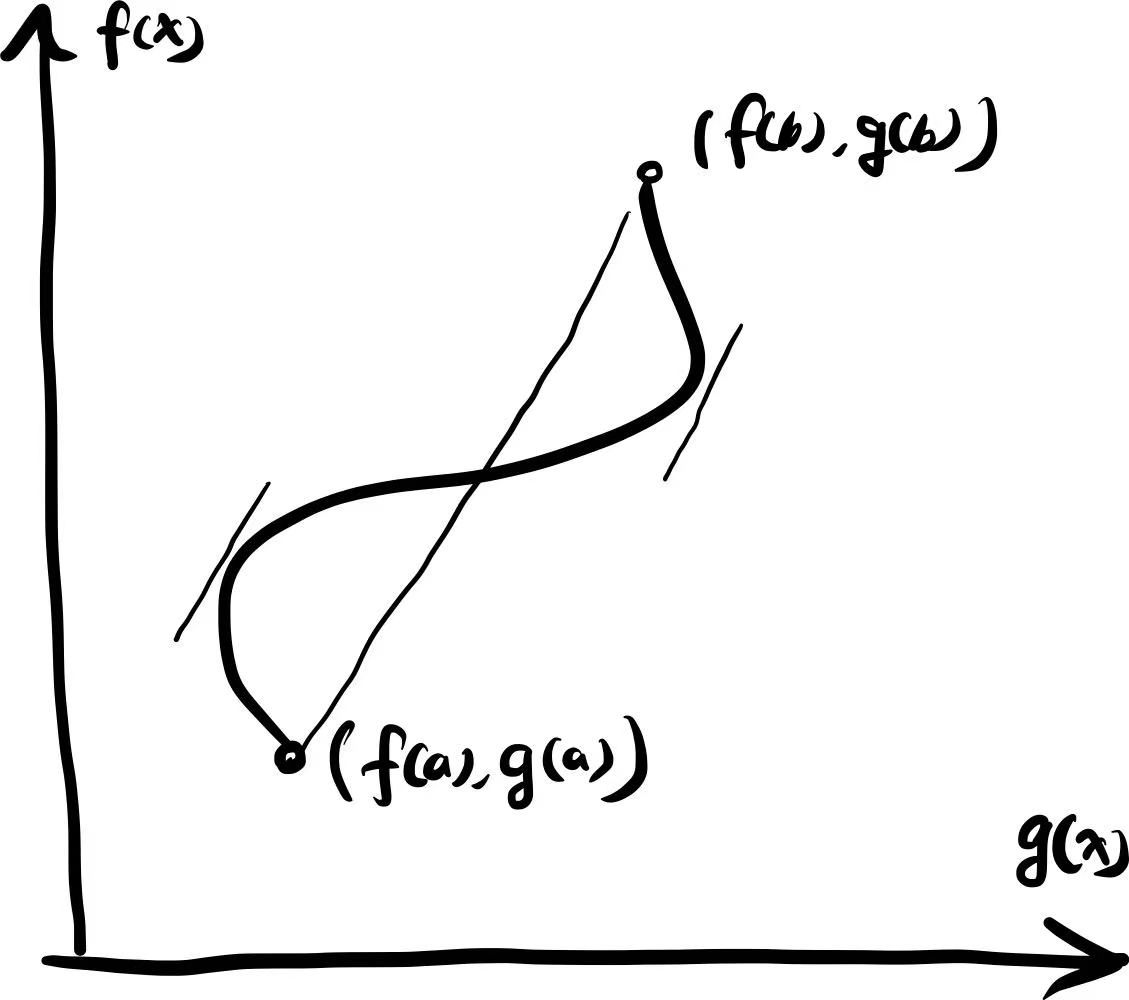
\includegraphics[width=0.9\textwidth]{img/image-20230615082658188.png}
\tcblower
\kaishu{\small 若 $f(x)$ 和 $g(x)$ 在区间 $[a,b]$ 连续, 且在区间 $(a,b)$
可微或存在导数, 且在区间 $(a,b)$ 内 $g(x)\neq0$, 则至少存在一个点
$x=c$ 使得 $\frac{f'(c)}{g'(c)}=\frac{f(b)-g(a)}{g(b)-g(a)}$.}
\end{tcolorbox}

\begin{newquote}
证明思路:

构造一个函数 $h(x):=f(x)-f(a)-\frac{f(b)-f(a)}{g(b)-g(a)}(g(x)-g(a))$
再利用拉格朗日中值定理易得上述结论.
\end{newquote}

为了理解这一条, 可以引入参数化曲线 (parametric curve) 这个概念.
一条曲线, 除了用类似 $y=f(x)$ 这样的形式来表示,
若是这条曲线是一个物体的运动曲线, 还可以引入时间 $t$, 这个参数
(parameter), 然后用时间来表示 $\{x,y\}$ 的变化, 即 \[
\begin{cases}
x=x(t),\\
y=y(t);
\end{cases}
\] 于是柯西中值定理可以视作, $f(x)$ 和 $g(x)$ 分别代表两个坐标值,
$x$ 是一个参数, 这样一来 $f'(x)/g'(x)$
就可以理解为这条参数化曲线的切线的''斜率''了.

\end{tcolorbox}

回到我们的主题, 当出现类似 $f(a)=0$, $g(a)=0$, 且希望求得极限
$\lim_{x\rightarrow a}\frac{f(x)}{g(x)}$ 时, 我们可以从 $a$
的某一侧逼近 $a$, 利用柯西中值定理可以知道在此区间一定存在一点 $x=c$
使得 \[
\frac{f'(c)}{g'(c)}=\frac{f(x)-f(a)}{g(x)-g(a)},
\] 已知 $f(a)=0$, $g(a)=0$, 于是 \[
\frac{f'(c)}{g'(c)}=\frac{f(x)}{g(x)},
\] 再令 $x\rightarrow a$, 因为 $c$ 一定在 $x$ 与 $a$ 之间,
于是类似三明治定理的情况, 在这个极限下, $c$ 也会趋向于 $a$;
于是我们便得到了我们希望得到的结果: \[
\boxed{\lim_{x\rightarrow a}\frac{f(x)}{g(x)}=\lim_{x\rightarrow a}\frac{f'(x)}{g'(x)}}.
\] 也就是说, 求极限时, 出现 $\frac{0}{0}$ 的不定式,
我们可以非常简单粗暴地来看它导数的极限.

\begin{newquote}
例: $\lim_{x\rightarrow 0}\frac{\sin(x)}{x}$ \[
\lim_{x\rightarrow 0}\frac{\sin(x)}{x}\underset{\text{L.H.}}{=}\lim_{x\rightarrow 0}\frac{\cos(x)}{1}=1.
\]
\end{newquote}
\hypertarget{ux6cf0ux52d2ux7ea7ux6570}{%
\subsubsection{泰勒级数}\label{ux6cf0ux52d2ux7ea7ux6570}}

\textbf{求和 (summation) - 复习}

求和的标记 \[\sum\] 在【007】其实已经介绍过了, 这里再复习一遍.
求和符号右边是代求和的每一项的表达式,
求和符号下面标注了右边表达式的第一项需要代入的值,
求和符号上面则标注了最后一项需要代入的值.

\begin{quote}
举一个例子, 小学的高斯求和法, \[
1+2+...+99+100=\sum_{n=1}^{100}n=5050.
\] 高斯的思路无非是, 将这个求和拆为 \[\{1,100\}\], \[\{2,99\}\], \ldots,
\[\{49,52\}\]\[, \{50,51\}\] 的组合, 每一组的和都是 \[101\], 一共有
\[50\] 个这样的组合, 于是得到''一加到一百''为 \[5050\] \footnote{小学高我一年级的一学长刚学完这一课向我耍宝的时候,
  其实我也想到了类似的方法, 把求和凑成 \[\{1,99\}\], \[\{2,98\}\],
  \ldots, \[\{48,52\}\]\[, \{49,51\}\] 的一对对, 最后还剩下 \[50\] 和
  \[100\], 也能得到答案, 不过这个方法并不普适.}.
推广一下便可得到对一组公差为 \[1\] 的等差数列求和,
和为【首项】加【末项】乘【项数】除以二. 于是有 \[
\sum_{n=1}^Nn=\frac{N(N+1)}{2}.
\] 另有两个可能会有一些用的结论: \[
\begin{aligned}
  \sum_{n=1}^Nn^2&=\frac{N(N+1)(2N+1)}{6},\\
  \sum_{n=1}^Nn^3&=\left(\frac{N(N+1)}{2}\right)^2.
\end{aligned}
\] 证明留作练习, 提示是可以利用数学归纳法 (参见【007】).
\end{quote}

因为前面提到过, 这并不是一本严谨的数学书, 数列和级数我们就跳过了;
但是接下来要讲泰勒级数, 还是来一点开胃菜 (appetizer): \textbf{几何级数}
(geometric series).

几何级数又叫等比级数, 即它的每一项和之前一项的倍数是恒定的. 于是第一项为
\[a\], 相邻两项倍数为 \[r\] 的几何级数可以记作 \[
\sum_nar^{n-1}.
\] 不难证明前 \[n\] 项之和应为 \[
S_n=a\frac{r^n-1}{r-1}.
\]

\begin{quote}
上结论证明如下:

前 \[n\] 项之和展开写是 \[S_n=a+ar+ar^2+...+ar^{n-2}+ar^{n-1}\],
两边同乘 \[r\] 得到 \[rS_n=ar+ar^2+ar^3+...+ar^{n-1}+ar^n\]. 将 \[rS_n\]
与 \[S_n\] 相减, 消去相同项便有 \[(r-1)S_n=a(r^n-1)\],
整理便可得到结论.\footnote{在这个推导中, 可以看到我们将代求的 \[S_n\]
  带着计算, 要习惯这种和逆向思维相对的''正向思维'',
  【014】逆函数的导数的推导也有这么一丝味道,
  【剧透警告】之后积分中非常重要的分步积分法也会有类似的思路.}
\end{quote}

这样一来, 当这个级数无限长, 即 \[n\] 趋向于无穷, 且公倍数 \[r\]
的绝对值小于一, 这个级数 (求和) 收敛到 \[
\sum_nar^{n-1}=\frac{a}{1-r}.
\] \textbf{泰勒级数 (Taylor Series)}

有的时候, 我们研究的函数 \[f(x)\] 可能并不是一个非常 nice 的函数,
它的很多特性并不那么''好''; 更直观一些,
很多时候我们研究的函数可能是\textbf{超越函数} (Transcendental
Functions), 即变量之间的关系不能用有限次加, 减, 乘, 除,
次方运算表示的函数, 最简单的例子, 比如三角函数, 不利用计算器等工具,
我们很难去直接计算. 正好, 很多现实场景下, 我们也并不需要任意精确的结果,
我们可能只需要几位有效数字, 这个时候,
我们便可以利用那些''好''的函数去\textbf{拟合} (fit)
这些不那么''好''的函数.

最常见的比较''好''的函数是什么? 多项式 (Polynomial)! 它取值相对简单,
对它求导更是非常轻松. 所以很多时候, 我们会用多项式去拟合.

现在假设我们手头上有一个函数 \[f(x)\], 我们希望能用多项式去拟合它,
那么它大约可以被写成以下的形式:

\[
f(x)=\sum_{n=0}^\infty a_n(x-x_0)^n,
\]

这里 \[a_n\] 是每一项的系数, \[x_0\] 是某个固定的值, 可以看到 \[x\]
的最高系数逐项增加. 对上式不断求导可以得到

\[
\begin{gather*}
f'(x)=a_1+2!\cdot a_2(x-x_0)+\mathcal{O}(x-x_0)^2\\
f''(x)=2!\cdot a_2+3!\cdot a_3(x-x_0)+\mathcal{O}(x-x_0)^2\\
...
\end{gather*}
\]

仅在这里, 我们规定 \[\mathcal{O}\] 的含义是, 例如: \[\mathcal{O}(x)\]
表示包含 \[x\] 以及 \[x\] 更高次数的项 (即, \[ax, bx^2, cx^3, ...\] ).
通常而言, \[n\] 次导可以得到:

\[
f^{(n)}(x)=n!a_n+\mathcal{O}(x-x_0)
\]

令 \[x:=x_0\] 便可得到每一项系数应该是

\[
a_n=\frac{f^{(n)}(x_0)}{n!},
\]

于是用来拟合一个函数的多项式便可以是

\[
\boxed{f(x)=\sum_{n=0}^\infty\frac{f^{(n)}(x_0)}{n!}(x-x_0)^n.}
\]

将一个函数用上式展开, 便得到了这个函数的\textbf{泰勒级数}\footnote{剧透:
  把这个结论推广到复变函数, 泰勒级数就变成了\textbf{洛朗级数 (Laurent
  series)}.}. 【007】中提到的二项式展开,
其实可以看做是泰勒级数的一个特例.

\textbf{收敛性}

前面我们似乎是假定随着项数增加泰勒级数可以趋向原函数了, 但是一定如此吗?
这边有一个定理.

\textbf{泰勒中值定理 (Taylor's Theorem)}

有一个 \[n\] 次可导的函数 \[f(x)\], 将其的导数依次记作
\[f'(x),f''(x),...,f^{(n)}(x)\], 考虑一个闭区间 \[[a,b]\],
那么在这个区间内一定存在一个 \[c\] 使得 \[
f(b)=f(a)+f'(a)(b-a)+\frac{f''(a)}{2!}(b-a)^2+...+\frac{f^{(n)}(c)}{n!}(b-a)^n.
\] 注意等式右边前面的函数和导数都是在 \[x=a\] 处取值, 而最后一项是在
\[x=c\] 处. 不难看出这其实是中值定理的推广.

如此一来, 换言之, \[f(x)\] 与
\[f(x_0)+f'(x_0)(x-x_0)+...+\frac{f^{(n-1)}(x_0)}{(n-1)!}(x-x_0)^{n-1}\]
的偏差等于 \[\frac{f^{(n)}(\xi)}{n!}(x-x_0)^n\], 对于某个在 \[x\] 和
\[x_0\] 之间的 \[\xi\].

实际使用的时候, 我们常常这么说: 【在 (某个特定的) \[x_0\] 附近展开
\[f(x)\] \ldots】 这样一来, 就要注意, 展开后,
取\textbf{有限项}级数来\textbf{近似}原函数时, 只有取 \[x\]
\textbf{足够}接近 \[x_0\] 时才是有效的. 例如: 利用在 \[0\] 附近展开的
\[\sin(x)\] 函数的泰勒级数的前若干项, 来近似当 \[x\] 很大时 (例如大于
\[2\pi\]) 时, 结果会是非常荒谬的\footnote{一些体外话: 在计算科学,
  数据分析等专业, 当我们有许多数据点,
  经常会用多项式去试图拟合这一些数据点, 更高次的多项式,
  通常意味着对已有数据更好的拟合 (比如 \[n\] 次的多项式可以完美拟合
  \[(n+1)\] 个数据点), 但是这往往并不是我们想要的,
  一方面在所有数据点两端, 高次多项式的行为会非常不合理, 另一方面,
  事实上一个模型也不应该具有如此高的自由度 (多项式每高一次,
  对应着模型多一个自由度). 这就引出了两个概念: 插值 (interpolation)
  vs.~拟合 (fitting), 插值要求函数通过每一个给定的数据点,
  而拟合是在现有模型的基础上调整参数, 保证函数和数据点是最小二乘的
  (least squared).}; 这里可以利用 \[\sin(x)\] 函数的周期性, 将 \[x\]
减去若干个 \[2\pi\] 再计算.

\textbf{练习}

求以下函数的泰勒级数: (a) \[(1\pm x)^{-1}\], (b) \[\mathrm{e}^x\], (c)
\[\sin(x)\], (d) \[\cos(x)\], (e) \[\ln(1+x)\], (f) \[\arctan(x)\].

展开后不难发现, 对于 \[x\approx 0\] (或者说 \[x\ll1\]) 有
\[\sin(x)\approx x\], \[\cos(x)\approx 1\] (当 \[x\] 足够小, 含 \[x\]
及其高次的项便足够小, 回收了【009】中提过的小角度近似).
另外还有一个常用的近似是 \[\ln(x+1)\approx x\] 对于 \[x\ll 1\]. 在还有,
展开的形式可以进一步地佐证欧拉公式 (回顾【009】).

\section{积分}\label{017}

来到微积分的积分. 首先是动机 (motivation), 为什么需要积分?
我们需要导数或者说微分是通常是因为我们需要知道一些物理量的\textbf{变化率}
(rate of change), 当然之前提到的求切线也可以作为一个非常 trivial
的一个情况. 积分呢, 图像上来说, 积分往往反映的是函数图像与
$x$-轴围起来的面积; 这里要注意, 不要被这种可视化个梏桎住了思想,
就像切线只是导数的一种可视化一样,
函数图像下方的面积也仅仅只是积分众多的可视化的一种,
不能局限于这一层理解.

\begin{tcolorbox}[size=fbox, breakable, enhanced jigsaw, title={积分 (integration)}]

若有一个函数 $f(x)$, 我们希望求得它在 $[a,b]$ 这个区间内, 函数图像与
$x$-轴 (左右再加两条竖线) 围成的面积; 如下图所示,

\begin{itemize}
\item
  首先我们可以尝试用一个个矩形去近似代求的面积, 在 $[a,b]$
  之间选取一系列的点, 使得 $a=x_0<x_1<x_2<...<x_{n-1}<x_{n}=b$,
  于是便有了一系列形如 $[x_i,x_{i+1}]$ 的子区间 (subinterval);
  这称之为一个分割 (partition);
\item
  直觉上, 如果将子区间进一步地分割, 或者专业一点的说: 如果有更精细
  (fine) 的分割, 矩形会更加贴合函数曲线, 即近似地误差会变得更小,
  矩形的面积之和会更接近函数围成的实际面积;
\item
  当每一个子区间的``宽度''趋向于 $0$ 时,
  直觉上矩形的面积之和便会趋向于函数围成的实际面积.
\end{itemize}


\begin{tcolorbox}[size=fbox, breakable, enhanced jigsaw]
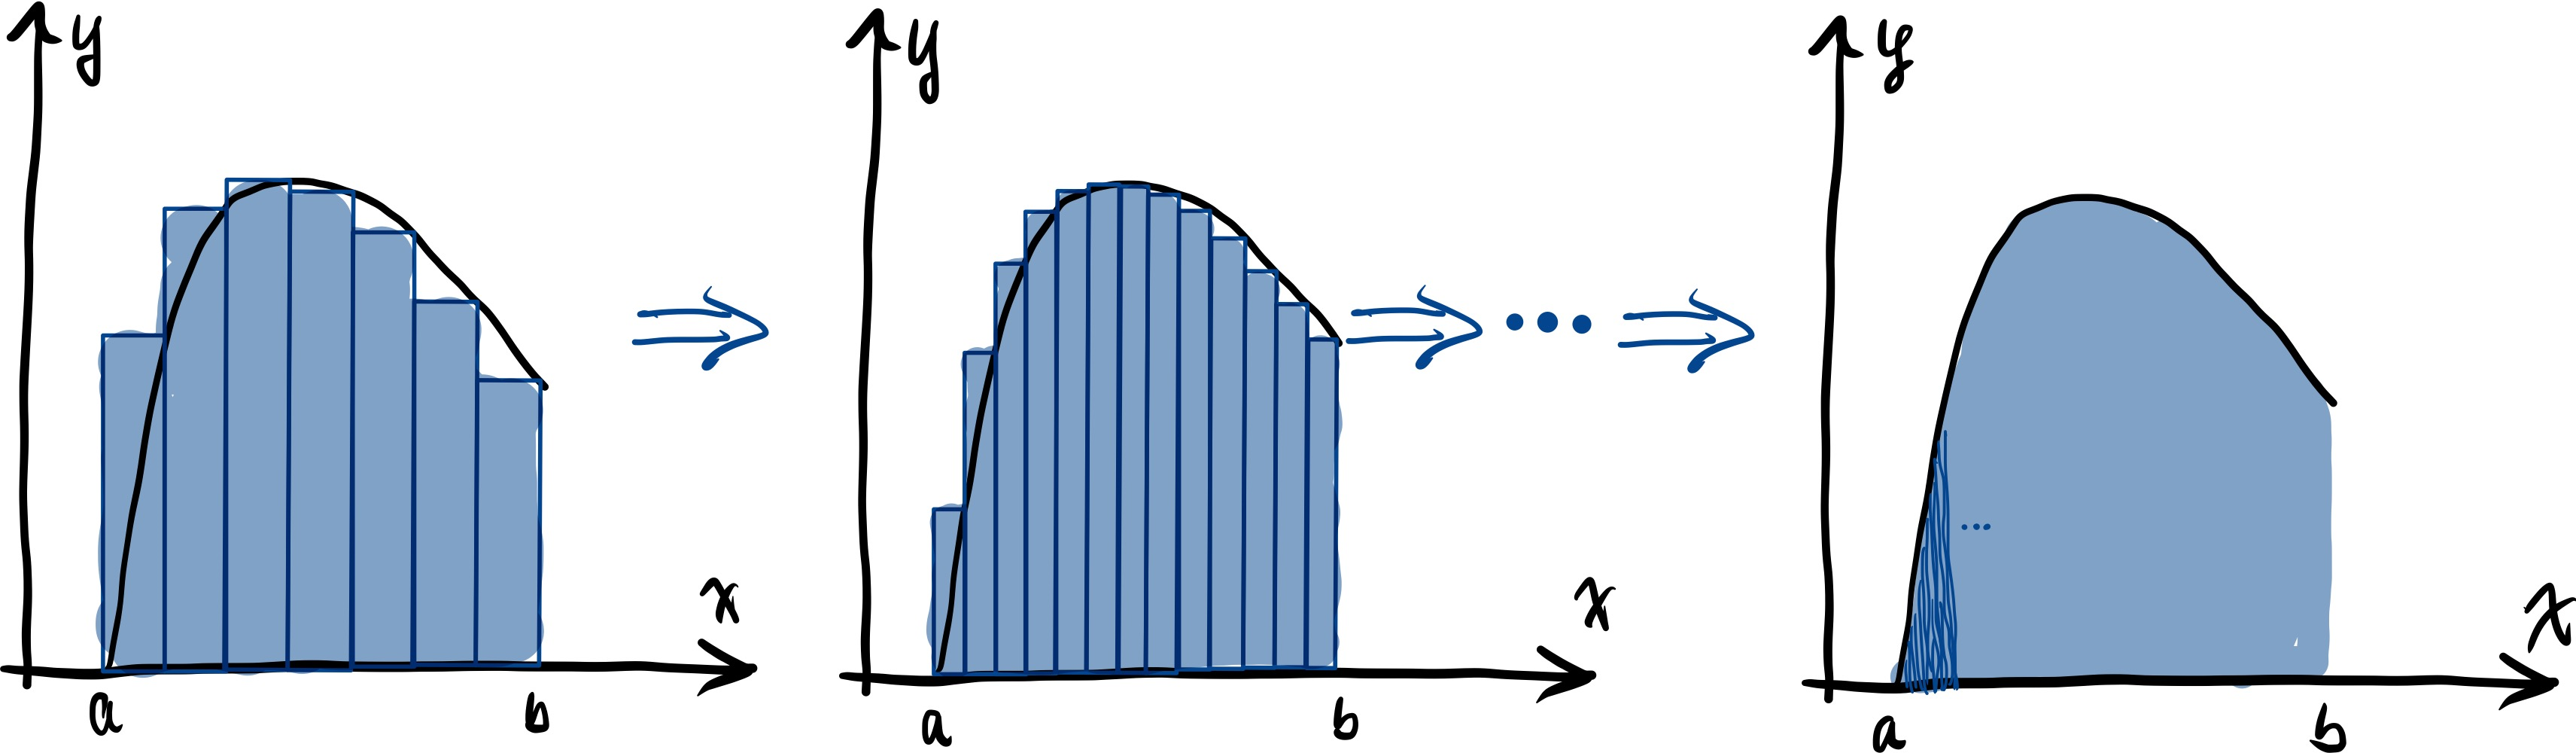
\includegraphics[width=0.9\textwidth]{img/image-20230906163643414.png}

\end{tcolorbox}

正式一点的, 我们把这些矩形面积和称作黎曼和 (Riemann sum): \[
\sum_{i=0}^{i=n-1}f(\xi_i)(x_{i-1}-x_i),
\] 其中 $x_{i-1}\le\xi_i\le x_i$. 当分割不断变得更加精细,
黎曼和最终趋向的值, 我们称其为函数 $f(x)$ 在区间 $[a,b]$
的\textbf{定积分} (definite integral), 暂时将这个值记作 $I$,
对于任意的 $\epsilon>0$ 都有 $\delta>0$ 使得: 对于任意的分割,
子区间的数量 $n<\delta$, 以及任意选择的每一个 $\xi_i$ , 我们有: \[
\left|\sum_{i=0}^{i=n-1}f(\xi_i)(x_{i-1}-x_i)-I\right|<\epsilon.
\] 我们可以将定积分定义为, \[
\boxed{I=\lim_{n\rightarrow\infty}\sum_{i=0}^nf(\xi_i)(x_{i+1}-x_i).}
\] 令 $\Delta x:=x_{i+1}-x_i$, 这样一来,
上面取子区间的数量趋向无穷的极限一定程度上等价于每个子区间的``宽度''趋向于无穷小,
于是在这个极限下 $\Delta x$ 变成了一个无穷小量, 即
$\Delta x\rightarrow \mathrm{d}x$\footnote{这个操作在物理中经常出现,
  要很熟悉这种找到有限的变化之间的关系, 然后令它变为无穷小量这样的操作.}.
对此, 莱布尼兹 (Leibniz) 发明了一个定积分的标记,
他将一个``S''拉长表示这种特殊的``求和'', 于是上面的定积分我们便通常写作
\[
\boxed{\int_a^bf(x)\mathrm{d}x.}
\] 有一点要注意的是, 这个积分之和函数本身 $f$, 积分的区间 $[a,b]$
相关, 和积分对象 $x$ 无关, 所以将定积分的积分对象由 $x$
换为其他任意字母, 得到的结果是不变的. 于是在这种情况下, 像 $x$
这样出现在公式中, 但又不实际太多地参与到运算中的变量,
我们称之为虚拟变量/哑变量 (dummy variable,
个人认为傀儡变量更信雅达一些).

\begin{newquote}
很多初学者最早在接触积分的时候, 会忘记最后的 $\mathrm{d}x$,
本人最初的理解是, 这个 $\mathrm{d}x$ 是用来表示积分对象是 $x$;
但从函数图像面积这样的几何角度出发, 这个 $\mathrm{d}x$
事实上是每一个子区间面积的``底'', 因此这个 $\mathrm{d}x$
是不能被省略的.
\end{newquote}

\end{tcolorbox}

\begin{tcolorbox}[size=fbox, breakable, enhanced jigsaw, title={更加严格的版本 - 选读}]

对于某一个特定的分割, 在子区间 $[x_{i-1},x_i]$ 中, 令
\begin{gather*}
M_i:=\sup \left(f(x)\right),\\
m_i:=\inf \left(f(x)\right).
\end{gather*}

\begin{newquote}
这里 $\sup$ 和 $\inf$ 全写是 supremum 和 infimum,
中文分别是上确界和下确界, 和最大值 $\max$ 和最小值 $\min$ 很像,
区别在于, 例如在某个区间内, 若 $f(x)\le \eta$, 我们可以说
$\eta=\max \left(f(x)\right)=\sup \left(f(x)\right)$, 但若
$f(x)<\eta$, 我们只能说 $\eta=\sup \left(f(x)\right)$ 因为
$\max \left(f(x)\right)$ 取不到 $\eta$.
\end{newquote}

再令
\begin{gather*}
U:=\sum M_i\Delta_i,\\
L:=\sum m_i\Delta_i,
\end{gather*}
相当于某一个特定的分割下, 黎曼和的上限和下限, 最后令
\begin{gather*}
\overline{\int_a^b}f(x)\mathrm{d}x:=\inf U,\\
\underline{\int_a^b}f(x)\mathrm{d}x:=\sup L,
\end{gather*}
即所有分割下, $U$ 的下限和 $L$ 的上限 (上限的下限和下限的上限,
lol), 分别称他们为黎曼上积分和黎曼下积分.
若一个函数在一个区间内黎曼上积分和下积分相等,
我们就说这个函数在这个区间内是黎曼可积的 (Riemann integrable),
积分的值记作 $\int_a^bf(x)\mathrm{d}x$.
\end{tcolorbox}
\section{微积分基本定理-上}\label{018}

\begin{tcolorbox}[size=fbox, breakable, enhanced jigsaw, title={微积分基本定理 (fundamental theorem of calculus)}]

前面只讲了积分的动机和定义, 但是并没有涉及具体的运算,
那么这里先摆出结论: 积分和微分可以视作互逆的运算.
这一点在很多高中的教材似乎是默认的, 但是事实上真的如此吗?
为了证明这一点, 首先, 令 \[
F(x):=\int_a^xf(\xi)\mathrm{d}\xi,
\]

\begin{newquote}
怎么突然出现了 \(\xi\) ? 其实原则上写 \(f(x)\mathrm{d}x\)
也没有太大问题, 但是积分的上限也是 \(x\), 为了加以区分,
所以将积分对象的变量改为其他字母, 其含义是没有发生任何变化的
(参见\ref{017}\nameref{017}对于 dummy variable 的讨论). 只是积分对象和积分上限都用
\(x\) 有滥用标记 (abuse of notation) 之嫌, 不是非常专业.
\end{newquote}

考虑 \(F(x)\) 的斜率, 首先是近似的形式 \[
\begin{aligned}
&\frac{F(x+h)-F(x)}{h}\\
=&\frac{1}{h}\left(\int_a^{x+h}f(\xi)\mathrm{d}\xi-\int_a^xf(\xi)\mathrm{d}\xi\right)\\
=&\frac{1}{h}\int_x^{x+h}f(\xi)\mathrm{d}\xi.
\end{aligned}
\] 上式最后两行可以如下图所示地用函数下的面积来理解,
不难看出第一个积分得到的是深色面积,
第二个积分得到的是深色和浅色的面积之和, 于是他们的差便是浅色的面积,
浅色面积对应的区间是 \([x,x+h]\), 于是相当于是上下限分别是 \(x\) 和
\((x+h)\) 的积分.

\begin{tcolorbox}[size=fbox, breakable, enhanced jigsaw]
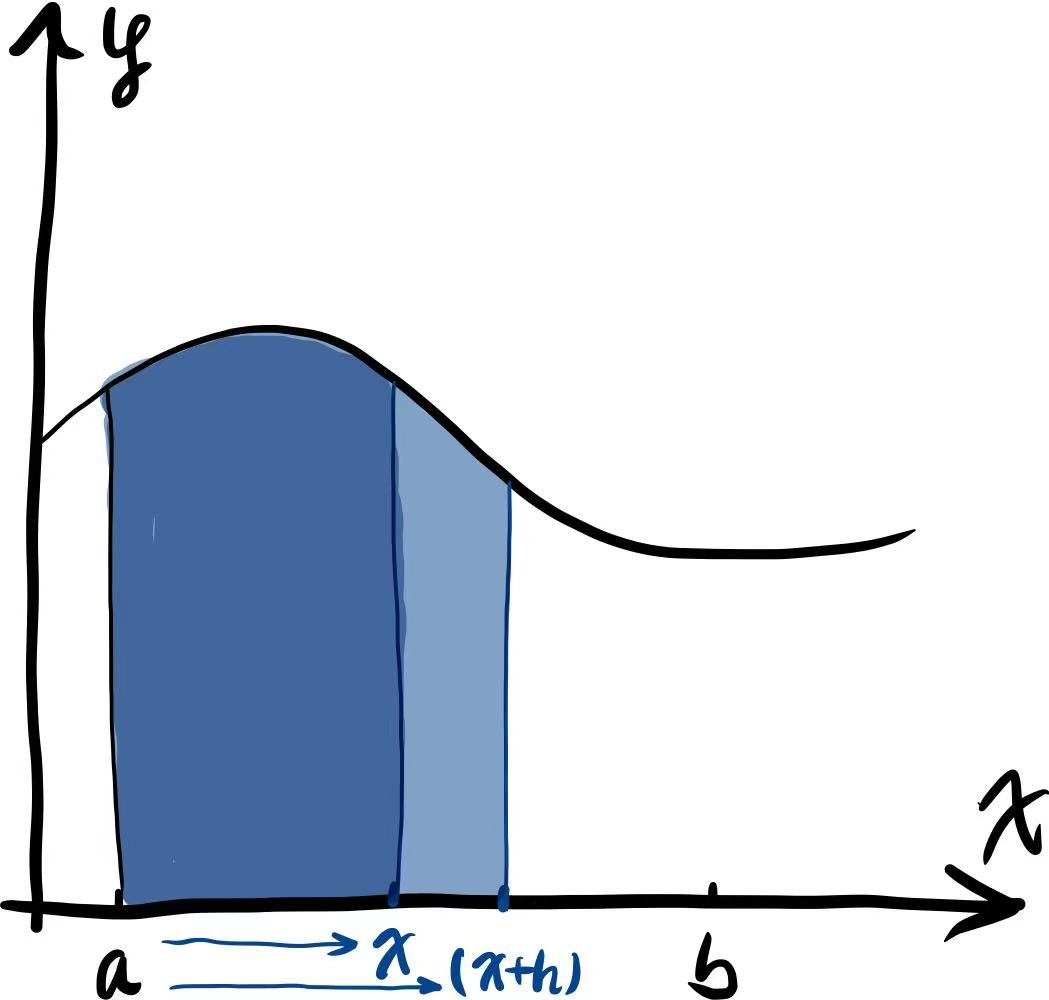
\includegraphics[width=0.3\textwidth]{img/image-20230912145204089.png}

\end{tcolorbox}

\begin{tcolorbox}[size=fbox, breakable, enhanced jigsaw, title={插曲: 定积分的中值定理}]\footnote{其实应该现有了微积分基本定理再推积分的中值定理会更方便,
  中值定理有 \(f'(c)=(f(b)-f(a))/(b-a)\) 对于某个区间 \([a,b]\) 内的
  \(c\). 令 \(F(x):=\int_a^xf(\xi)\mathrm{d}\xi\), 将 \(F(x)\)
  直接套入中值定理, 再利用积分和求导互为逆运算, 便有
  \(f(c)=F'(c)=(F(b)-F(a))/(b-a)\).}

若 \(f(x)\) 在区间 \([a,b]\) 连续, 则存在某点 \(c\) 使得, \[
\boxed{f(c)=\frac{1}{b-a}\int^b_af(x)\mathrm{d}x.}
\] 像 \(\frac{1}{b-a}\int_a^bf(x)\mathrm{d}x\) 这样的形式,
事实上是取了函数 \(f(x)\) 在区间 \([a,b]\) 的``平均值'', 即:
【把这个形式得到的值想象成高, 把 \([a,b]\) 想象成底,
相乘得到的矩形面积】和【积分对应的函数图像下的面积】应该是一致的;
那么自然, 这个``平均值''是小于这个区间内 \(f(x)\) 的最大值,
而大于这个区间内 \(f(x)\) 的最小值的; 同时, 因为 \(f(x)\) 是连续的,
那么必然在这个区间内存在至少一点 \(c\) 使得 \(f(c)\) 等于这个``平均值''.

\end{tcolorbox}

有了定积分的中值定理, 再对比一下前面 \(F(x)\) 的斜率的近似形式, 不难发现
\([x,x+h]\) 这个区间内, 也应该存在某点 \(c\), 使得
\(f(c)=\frac{1}{h}\int_x^{x+h}f(\xi)\mathrm{d}\xi\). 这里要注意, 这个
\(c\) 并不是固定的, 随着 \(h\) 的变化, \(c\) 应该也是随之变化的.

接下来的操作很不严谨的 (hand-wavy, 这边有一个很难直译的词,
当说一些很模棱两可又暧昧的说法时, 我们可能会习惯性地波动我们的手),
取极限 \(h\rightarrow0\) 是, 于是 \([x,x+h]\) 这个区间也越来越窄,
到最后迫使 \(f(c)\rightarrow f(x)\). 于是便有 \[
F'(x)=\lim_{h\rightarrow 0}\frac{1}{h}\int_x^{x+h}f(\xi)\mathrm{d}\xi=f(x).
\] 这便是\textbf{微积分基本定理} (fundamental theorem of calculus),
重新表述如下: \[
\boxed{\frac{\mathrm{d}}{\mathrm{d}x}\int_a^xf(\xi)\mathrm{\xi}=f(x).}
\] 可以看到, 一个函数经过积分又求导后变回了原函数,
可见微分和求导一定程度上确实应该是互为逆运算的. 这样,
当我们实际计算积分时可以利用\textbf{反导数 }(antiderivative) 来完成计算.

\begin{tcolorbox}[size=fbox, breakable, enhanced jigsaw, title={反导数}]

在某个区间内, 若对于任意 \(x\) 都有
\(F'(x)=\frac{\mathrm{d}}{\mathrm{d}x}F(x)=f(x)\), 则在此区间内函数
\(F(x)\) 是 \(f(x)\) 的反导数.

于是, 对于一个在区间 \([a,b]\) 内连续的函数 \(f(x)\), 它的定积分,
用微积分基本定理可以表述为: \[
\boxed{\int_a^bf(x)\mathrm{d}x=F(b)-F(a),}
\] 这里 \(F(x)\) 是 \(f(x)\) 在区间 \([a,b]\) 的反导数.

\end{tcolorbox}

\begin{newquote}
例: \(\int_a^b x\mathrm{d}x\)

我们知道, 求导时, 多项式的会先乘上次数, 然后次数会减一,
那么逆导数便应该是次数加一, 然后除以新的次数 (顺过来的运算后执行的,
逆运算先执行),

\begin{tcolorbox}[size=fbox, breakable, enhanced jigsaw]
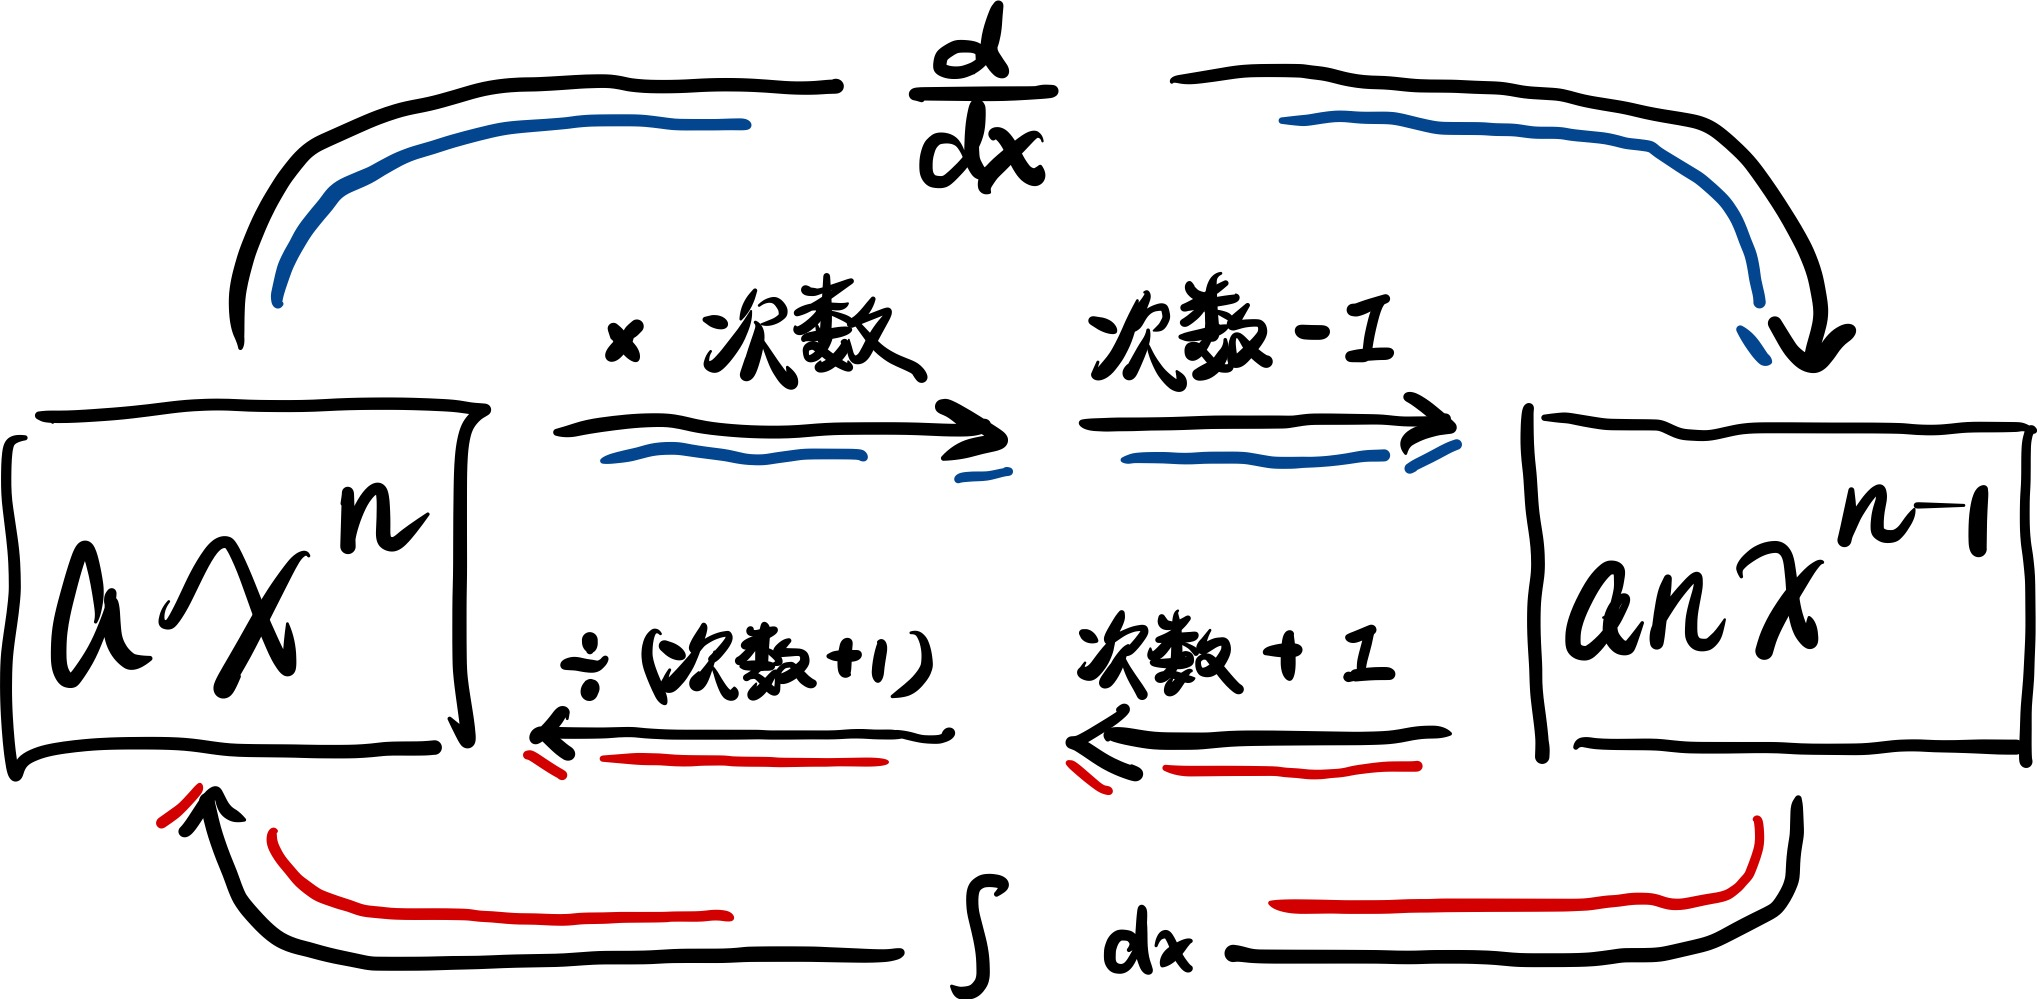
\includegraphics[width=0.6\textwidth]{img/image-20230912161734076.png}

\end{tcolorbox}

类似的, 三角函数, 指数函数, 对数函数, 符合函数 (复习链式法则,
参见\ref{013}\nameref{013}) 等等的逆导数也可以用这样的思路去求.

如此这般, 首先, 若 \(f(x)=x\), 应该对应逆导数 \(F(x)=\frac{1}{2}x^2\).
然后 \[
\begin{aligned}
  \int_a^bf(x)\mathrm{d}x&=F(b)-F(a)\\
  &=\frac{1}{2}b^2-\frac{1}{2}a^2.
\end{aligned}
\] 习惯上我们更通常这么写 \[
\begin{aligned}
\int_a^bx\mathrm{d}x=&\left.\frac{1}{2}x^2\right|_{x=a}^b\\
=&\frac{1}{2}b^2-\frac{1}{2}a^2.
\end{aligned}
\] 右边一竖的意思是在 \(x=a\) 和 \(x=b\) 处分别求值 (evaluate)
再求差的意思.
\end{newquote}

\begin{tcolorbox}[size=fbox, breakable, enhanced jigsaw, title={不定积分}]

前面积分时, 都强调了积分的上下限,
但是有的时候我们可能需要一个通常的表达式, 而不需要求值,
这种积分我们称作不定积分. 一个函数的不定积分等于它的逆求导加上一个常数:
\[
\int f(x)\mathrm{d}x=F(x)+\text{const.}
\] 等价的说法是, 一个函数其实并不只有一个逆导数,
但是这些逆导数只差了一个常数 (和积分变量无关). 这是因为求导时,
常数项直接``消失''了. 这就带来了规范自由 (gauge freedom)\footnote{超纲警告!
  规范自由本质上来说就是一个标量场加上一个常数并不会影响它的梯度.}.

\end{tcolorbox}
\end{tcolorbox}
\section{微积分基本定理-下}\label{019}

\begin{tcolorbox}[size=fbox, breakable, enhanced jigsaw, title={更加严格的版本 - 选读}]

考虑一个在区间 \([a,b]\) 可积的 \(f(x)\), 和先前一样的, 令 \[
F(x):=\int_a^xf(\xi)\mathrm{d}\xi,
\] 这里 \(a\le x \le b\). 考虑 \(f(x)\) 在此区间的上下界, 若有
\(M\ge |f(x)|\) 在此区间内, 那么对于 \(a\le p \le q \le b\) 显然有 \[
|F(q)-F(p)|=\left|\int_p^qf(\xi)\mathrm{d}\xi\right|\le M\cdot(q-p).
\] (如果觉得不那么显然的话, 可以参考\ref{018}\nameref{018}``平均值''这一套论述).
于是对于 \(\epsilon>0\), 只要\(|q-p|<\epsilon/M\), 便有
\(|F(q)-F(p)|<\epsilon\), 这样首先证明了 \(F(x)\) 是连续的.

继而, 选定某个 \(x\), 且在此处 \(f(x)\) 是连续的. 给定 \(\epsilon>0\),
选择一个 \(\delta>0\), 使得若有 \(|\xi-x|<\delta\) 且 \(a\le\xi\le b\),
便有 \(|f(\xi)-f(x)|<\epsilon\).

如此一来, 如果 \(x-\delta<p\le x\le q<x+\delta\), 且 \(a\le p<q\le b\),
便有 \[
\begin{aligned}
\left|\frac{F(q)-F(p)}{q-p}-f(x)\right|&=\left|\frac{1}{q-p}\left(\int_a^qf(\xi)\mathrm{d}\xi-\int_a^pf(\xi)\mathrm{d}\xi\right)-f(x)\right|\\
&=\left|\frac{1}{q-p}\int_p^qf(\xi)\mathrm{d}\xi-f(x)\right|\\
&=\left|\frac{1}{q-p}\int_p^q[f(\xi)-f(x)]\mathrm{d}\xi\right|\\
&<\left|\frac{1}{q-p}\int_p^q\epsilon\mathrm{d}\xi\right|=\epsilon.
\end{aligned}
\] 也就是说, 在区间 \([a,b]\) 有 \(F'(x)=f(x)\). 以上我们用
\(\epsilon-\delta\) 语言更严格地证明了某种意义上, 积分和微分互为逆运算.

类似的, 尝试证明对于任意 \(\epsilon>0\) 都有
\(\left|F(b)-F(a)-\int_a^bf(x)\mathrm{d}x\right|<\epsilon\),
也可以严格证明定积分的微积分基本定理, 这一部分留作练习.

\end{tcolorbox}

\begin{tcolorbox}[size=fbox, breakable, enhanced jigsaw, title={应用? - 和物理的联系}]

经典的速度的定义是位移的导数,
\(v\equiv \frac{\mathrm{d}}{\mathrm{d}t}s(t)\).

如下图所示: 匀速的情况, 位移很好理解, 无非是速度乘上时间.
速度是阶梯函数的话, 位移依旧很好求, 分段计算即可.
若速度是连续变化的函数, 那么在我们有积分这个工具之前, 就非常困难了.

\begin{tcolorbox}[size=fbox, breakable, enhanced jigsaw]
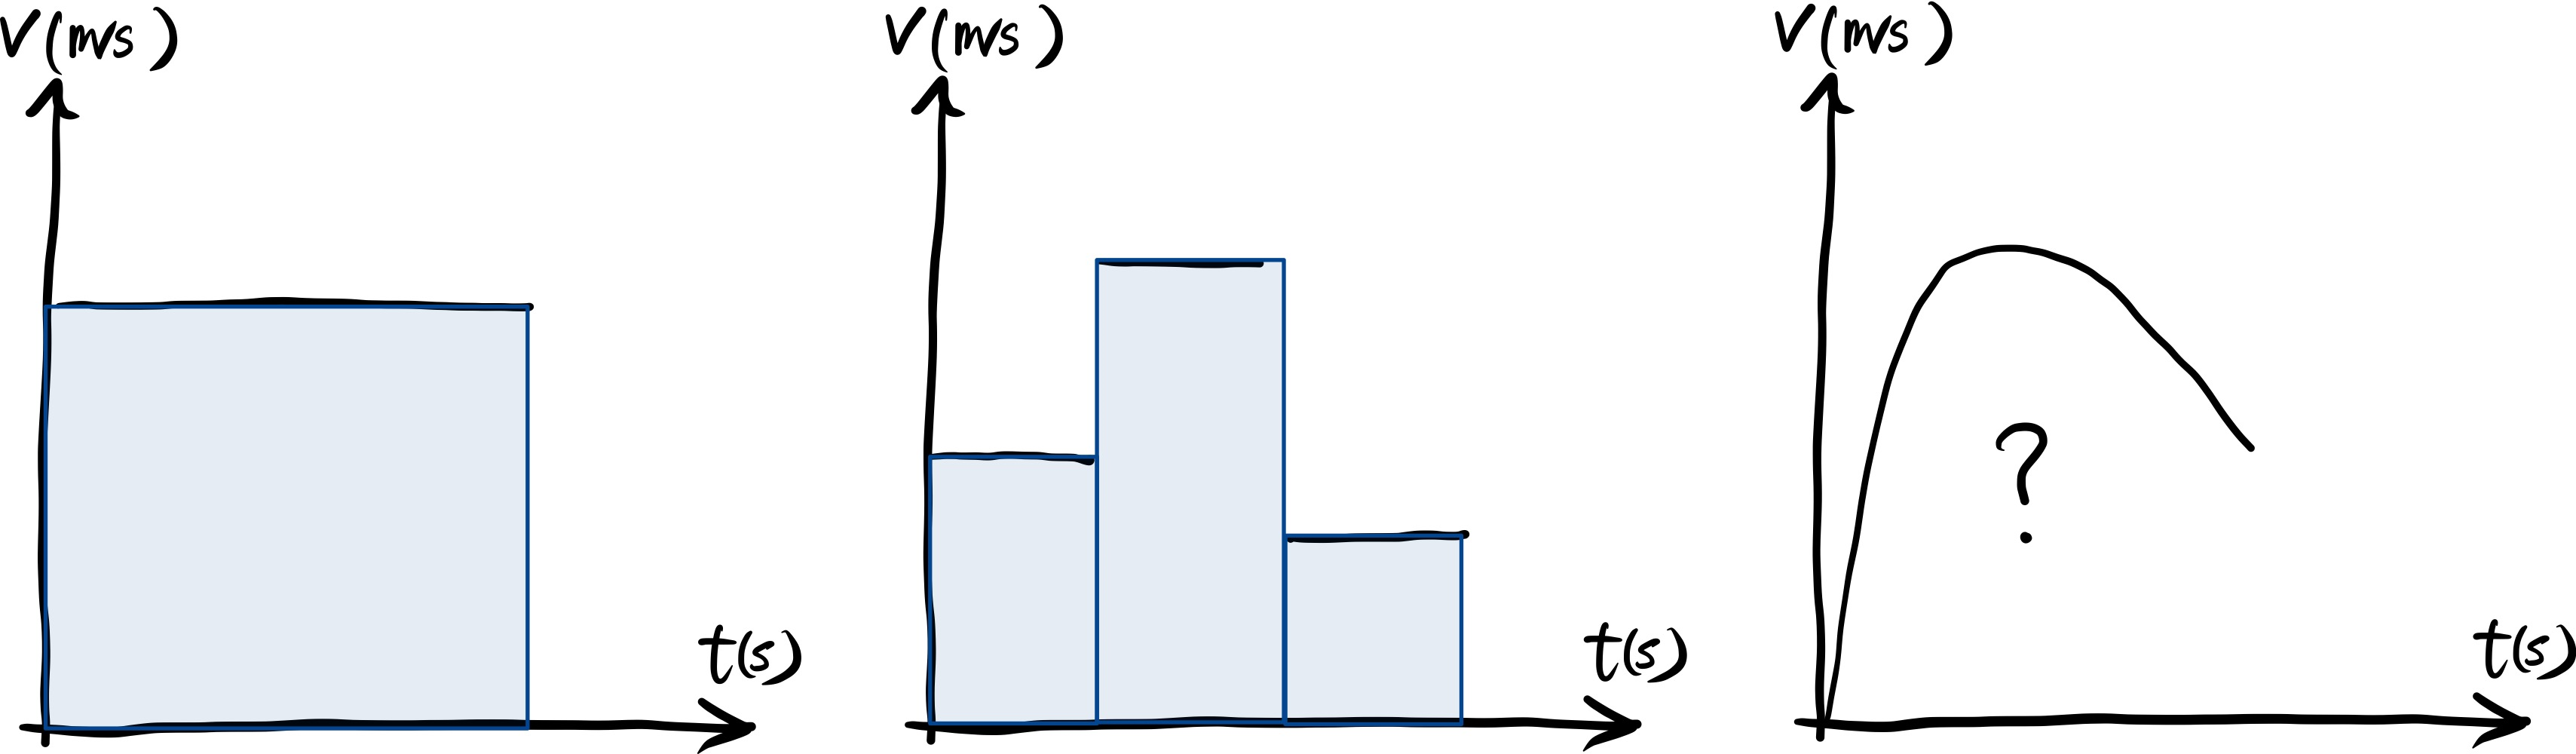
\includegraphics[width=0.9\textwidth]{img/image-20230912164801681.png}
\end{tcolorbox}

我们可以尝试将整个过程分成很多段, 每一段估计一个平均速度
(这一段时间内最大速度和最小速度之间的值), 然后把这一段近似成匀速计算,
或者将这一小段近似成匀变速的情况, 即 \(s=ut+\frac{1}{2}at^2\)
(如果没见过这个公式可以忽略它\ldots{} 不影响后面的理解). 不管怎么样,
对于匀速和速度是阶梯函数, 我们其实还是计算了\(v-t\)函数图像下的面积,
对于速度是连续函数的情况, 我们也还是在估算函数下方的面积, 于是很自然的,
若我们有积分这个工具, 速度又可以表示成一个关于时间的函数, 应该有 \[
s=\int v\mathrm{d}t.
\] 当然, 不定积分需要加上积分常数 (参见\ref{018}\nameref{018}文末),
这通常可以靠初始条件 (比如 \(t=0\) 时的位移) 来确定;
定积分反映的则是两个时间点之间发生的位移. 类似的,
既然加速度的定义是速度的变化率 (导数),
\(a\equiv \frac{\mathrm{d}}{\mathrm{d}t}v(t)\), 那么也应该有 \[
v=\int a\mathrm{d}t.
\] 当然, 也要注意不定积分需要用初始条件确定积分常数,
而不定积分反映的是两个时间点之间速度的变化量.

再还有很多情况:

\begin{itemize}
\item
  比如力时关于位置的一个函数, 那么做功就不再是简单的 \(W=Fx\), 而是
  \(W=\int F(x)\mathrm{d}x\) 了;
\item
  比如密度是关于位置的函数, 那么质量就不再是简单的 \(m=\rho V\), 而是
  \(m=\int \rho(\vec{r})\mathrm{d}V\), 这个体积微元 (volume
  differential/infinitesimal) 实际运算的时候需要计算三重积分, 即
  \(\int\cdot\mathrm{d}V=\iiint\cdot\mathrm{d}x\mathrm{d}y\mathrm{d}z=\iiint\cdot r^2\sin\theta\mathrm{d}r\mathrm{d}\theta\mathrm{d}\phi\),
  这里给的是三维直角坐标系和球状坐标系的例子,
  视情况和方便程度而定使用哪种坐标, 这里暂时不具体展开.
\end{itemize}
\end{tcolorbox}
\section{积分技巧}\label{020}

\begin{tcolorbox}[size=fbox, breakable, enhanced jigsaw, title={换元 (substitution)}]

事实上积分时的换元就是求导时的链式规则 (参见\ref{013}\nameref{013}) 反过来的过程.
具体操作是这样的, 例如若代求 \(\int f(x)\mathrm{d}x\), 有时为了计算方便,
我们 (i) 先定义另一个函数 \(u(x)\), 并利用 \(f(x)\) 和 \(u(x)\) 的关系,
将代积分的部分的 \(x\) 消去, 将其变为一个关于 \(u\) 的函数; (ii)
因为现在积分的对象不显含 \(x\) 了, 因此我们应该将最后的 \(\mathrm{d}x\)
也尝试变为 \(\mathrm{d}u\) (乘上一些项); 实际操作中 (i) 和 (ii)
步一般是同时进行的, 保证最后的形式是不显含 \(x\) 而只剩 \(u\); (iii)
最后, 若积分是一个定积分, 还要利用 \(x\) 和 \(u\) 的关系,
将积分上下限替换.

\begin{newquote}
例: 求 \(\int\sin^2(x)\cos(x)\mathrm{d}x\)

令: \(u=\sin(x)\)

则
\(\frac{\mathrm{d}u}{\mathrm{d}x}=\cos(x)\Rightarrow\mathrm{d}u=\cos(x)\mathrm{d}x\).

于是积分转化为 \(\int u^2\mathrm{d}u\), 后面的步骤便非常容易了.
\end{newquote}

\end{tcolorbox}

\begin{tcolorbox}[size=fbox, breakable, enhanced jigsaw, title={分部积分法 (integration by parts)}]

分部积分法是由求导的乘法法则 (参见\ref{012}\nameref{012}) 而来, 求导的乘法法则有 \[
(fg)'(x)=f'(x)g(x)+f(x)g'(x),
\] 对其积分可以得到 \[
\int(fg)'(x)\mathrm{d}x=\int f'(x)g(x)\mathrm{d}x+\int f(x)g'(x)\mathrm{d}x,
\] 等式左边也可以写成
\(\int\frac{\mathrm{d}}{\mathrm{d}x}f(x)g(x)\mathrm{d}x\),
根据微积分基本定理, 积分和求导可以视作互为逆运算, 于是等式左边事实上便是
\(f(x)g(x)\), 挪项可得 \[
\int f(x)g'(x)\mathrm{d}x=f(x)g(x)-\int f'(x)g(x)\mathrm{d}x.
\] 更通常的, 很多教材会使用 \(u(x)\) 和 \(v(x)\), 省略 \((x)\),
分部积分法可以记作 \[
\boxed{\int u\ \mathrm{d}v=uv-\int \mathrm{d}u\ v}.
\]

\begin{newquote}
注意: 上式中的 \(\mathrm{d}\cdot\) 并不表示积分对象是 \(v\) 和 \(u\),
例如 \(\int u\mathrm{d}v\) 要表示的事实上还是
\(\int u(x)v'(x)\mathrm{d}x\); 另外 \(\int \mathrm{d}u\ v\) 中的 \(v\)
也是需要被积分的, 这么记事实上非常不规范.

物理和工程上经常很类似的, 会有 \(\int\mathrm{d}x f(x)\) 这样的写法,
没有把代积分的部分夹在积分符号和 \(\mathrm{d}x\) 之间, 而把
\(\mathrm{d}x\) 前置, 某种程度上是先强调了一下积分的对象是哪一个变量.
\end{newquote}

实际计算中,
分部积分法经常出现在对于【一个函数和三角函数或是指数函数的乘积】的积分,
下面是一个例子.

\begin{newquote}
例: \(\int x\cos x\ \mathrm{d}x\)

这个积分是用先前的知识是无法直接进行的, 遂用分部积分法; 首先要规定 \(u\)
和 \(\mathrm{d}v\), 然后求 \(\mathrm{d}u\) 和 \(v\);
用部分积分法的时候要尽可能的让 \(\int \mathrm{d}u\ v\) 这一项方便计算,
因此这一题中, 我们选取 \(u=x\), 这样一来
\(\mathrm{d}u=1\cdot\mathrm{d}x\) 就很方便接下来的计算;
所以便有\footnote{下面这个盒子是我高中的数学老师 Paul Elkin 传授的,
  他把它称作 ``working block'' (工作区),
  当然习惯了之后可以完全省略这个盒子里的内容, 但是初上手的时候,
  这样一个盒子可以很好地把关键步骤和``计算草稿''分割开来,
  使得书写面板很整洁, 也方便检查.}: \[
\boxed{\begin{aligned}
&u=x,&&\mathrm{d}v=\cos x\ \mathrm{d}x;\\
&\mathrm{d}u=\mathrm{d}x,&&v=\sin x.
\end{aligned}}
\] 于是 \[
\int x\cos x\ \mathrm{d}x=x\sin x-\int\sin x\ \mathrm{d}x.
\] 后续的计算因为不包含两个函数乘积的积分就很容易了.

类似的, 一个多项式乘以三角函数或是指数函数都可以用上述方法;
有时分部积分后得到新的积分项还是无法直接进行,
这时便需要继续对这一项使用分部积分, 使得多项式不断降次.

还有一些情况也可以使用分部积分, 例如 \(\int\ln x\ \mathrm{d}x\),
乍一看似乎看不出这个积分的结果, 一个提示是可以把 \(\ln x\) 视作
\(1\cdot\ln x\), 后续的计算留作练习.
\end{newquote}

一些超纲: 事实上, 部分积分法的思想不止局限于对函数的积分, 在变分法
(calculus of variation) 中, 在推导欧拉-拉格朗日方程 (Euler-Lagrange
equation) 时, 对泛函 (functional)\footnote{函数从映射的角度,
  是将数映射到数, 这里的``数''可能是实数, 也可能是虚数, 还可以是向量
  (什么是向量? 后面再细讲); 而泛函, 可以理解为函数的函数,
  泛函可以将函数映射到数, 它的定义域是函数构成的向量空间
  (什么是向量空间? 有机会再细说), 值域一般是实数.} 也可以有类似的操作
(翻出了我本科的毕业论文中的一段) :

\begin{tcolorbox}[size=fbox, breakable, enhanced jigsaw]
  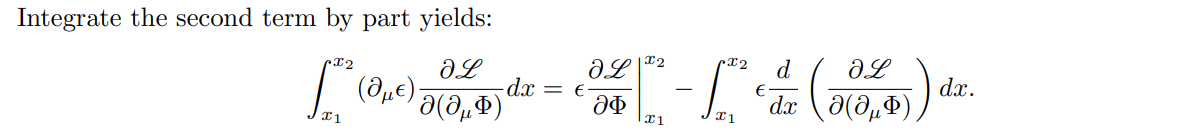
\includegraphics[width=0.9\textwidth]{img/image-20231101180718605.png}
\end{tcolorbox}

除此之外, 很多三角函数的积分可以利用三角函数的恒等式来化简;
两个多项式相除的积分可以利用部分分式 (partial fraction) 化简,
即将其变为若干个分式之和的形式; 更复杂的一些积分可以参考积分表,
作为一个现代人更可以合理使用一些计算软件辅助,
没有必要过分地去追求精通很多积分; 而且实际上,
很多积分并不能得到很好的解析式, 一般会用数值法来估算结果.
\end{tcolorbox}
\section{参数化曲线}\label{021}}

\ref{004}\nameref{004}中提到过用隐函数来表示一些图像, 事实上,
我们还可以利用\textbf{参数化曲线} (parametric curve)
来比较方便表示一些较为复杂的图像. 还是以圆形位于原点的圆作为一个 trivial
例子, \ref{005}\nameref{005}中我们简单地了解过极坐标, 不难发现, 圆周上的任意一点
\((x,y)\) 都可以写作 \((\cos\theta, \sin\theta)\); 于是, 我们可以将
\(\theta\) 视作圆的一个参数, 在 \(\theta\) 从 \(0\) 变为 \(2\pi\)
的过程中, 下面这一组函数便可绘出单位圆: \[
\begin{cases}
x(\theta)=\cos\theta\\
y(\theta)=\sin\theta
\end{cases}.
\]

如果希望求得这个函数某处的切线, 我们需要知道切线的斜率,
切线的斜率通常是通过 \(\frac{\mathrm{d}y}{\mathrm{d}x}\)求得的,
那么现在应该怎么办呢? 利用链式法则 (参见\ref{013}\nameref{013}) 可得 \[
\frac{\mathrm{d}y}{\mathrm{d}\theta}=\frac{\mathrm{d}y}{\mathrm{d}x}\frac{\mathrm{d}x}{\mathrm{d}\theta},
\] 所以我们可以先对前面的参数方程关于 \(\theta\) 求导,
然后利用下式得到其在某处的斜率 \[
\frac{\mathrm{d}y}{\mathrm{d}x}=\frac{\frac{\mathrm{d}y}{\mathrm{d}\theta}}{\frac{\mathrm{d}x}{\mathrm{d}\theta}}.
\]

\begin{newquote}
数学人震怒-1: 虽然不能这么理解, 但是为了记忆方便, 可以想象两个
\(\mathrm{d}\theta\) ``约掉了''.
\end{newquote}

\subsection{弧长}

弧长 (arc length) 和圆的弧长其实关系并不大,
这个词在这里被用来描述一个函数图像的一段曲线长度.
初一看可能函数图像的一段曲线长度很难被描述, 但是要注意,
我们现在已经有了微积分这一非常有力的工具, 我们可以从''极限'',
``微元''这些角度去思考. 这种思路在物理和工程上尤为重要,
当我们试图找到变量之间的微分关系时.

回到弧长, 当我们试图找到一段函数曲线的长度时, 我们可以先 zoom in (放大),
然后 focus on (观查) 其中非常小的一段, 当只关注其中非常小的一段时,
这一小段应该表现得足够线性 (如果不够线性, 那就是放大得还不够,
关注的区域不够小), 那么这一段弧长 \(\Delta l\)
应该可以利用勾股定理近似为 \(\sqrt{\Delta x^2+\Delta y^2}\),
然后取极限便有 \[
\boxed{\mathrm{d}l=\sqrt{\mathrm{d}x^2+\mathrm{d}y^2}}.
\] 当我们已知函数 \(y(x)\) 的情况下, 可以将上式改写为 \[
\mathrm{d}l=\sqrt{1+\left(\frac{\mathrm{d}y}{\mathrm{d}x}\right)^2}\mathrm{d}x.
\]

\begin{newquote}
数学人震怒-2: \textbf{相当于}把 \(\mathrm{d}x\) 提取出来了,
当然这么理解数学上是非常不严谨的, 但是物理和工程上 it just works.
\end{newquote}

于是, 在实际计算中, 若给定了函数 \(y(x)\),
其弧长便可以利用如下所示的积分计算 \[
l=\int\mathrm{d}l=\int\sqrt{1+\left(\frac{\mathrm{d}y}{\mathrm{d}x}\right)^2}\mathrm{d}x.
\]

\begin{newquote}
类似上式的思路在物理中很常见:

\begin{itemize}
\tightlist
\item
  比如对于质量分布不均匀的物体, 给定密度关于位置的函数 \(\rho(x,y,z)\),
  求质量, 利用 \(m=\rho V\) 便有:
  \(m=\int\mathrm{d}m=\int\rho(x,y,z)\mathrm{d}V=\iiint\rho(x,y,z)\mathrm{d}x\mathrm{d}y\mathrm{d}z\),
  这个积分的边界是这个物体的表面,
  所以最后一步的三重积分的上下限需要被非常小心地确定;
\item
  比如给定了电荷的分布, 求电场,
  利用\(E=\frac{Q}{4\pi\epsilon_0 r^2}\)有:
  \(\mathrm{d}E=\frac{1}{4\pi\epsilon_0}\frac{\mathrm{d}Q}{r^2}=\frac{1}{4\pi\epsilon_0}\frac{\rho}{r^2}\mathrm{d}V=\cdots\).
  当然, 严格来说这会是一个向量的积分, 暂时就不具体讲了.
\item
  \ldots{}
\end{itemize}

总而言之, 先从比较通常的情况 (质量均匀分布/点电荷/\ldots)
的变量关系出发, 然后一步步抽丝剥茧地将微元变为可以积分的变量为止
(\(\mathrm{d}m\Rightarrow \mathrm{d}V\Rightarrow\mathrm{d}x\mathrm{d}y\mathrm{d}z\))
.
\end{newquote}

那么如果给定的形式是一个参数化曲线呢? 例如, 已知 \(\{x(t),y(t)\}\),
那么可以先对 \(x(t)\) 和 \(y(t)\) 先分辨关于 \(t\) 求导, 得到
\(\mathrm{d}x\) 和 \(\mathrm{d}y\) 与 \(\mathrm{d}t\) 之间的微分关系,
然后弧长的微元便可以写作 \[
\mathrm{d}l=\sqrt{\left(\frac{\mathrm{d}x}{\mathrm{d}t}\right)^2+\left(\frac{\mathrm{d}y}{\mathrm{d}t}\right)^2}\mathrm{d}t.
\] 对其积分便可得到弧长.

\section{偏微分}\label{023}

\subsection{多变量函数}

先举一个偏日常的例子: 当我们看气象图的时候,
我们可以在地图上建立一个直角坐标系, 用类似 \((x,y)\)
这样的坐标来描述某地的位置, 每一个位置会对应一个温度 \(T\),
于是我们将两个实数映射到了一个实数
\(\mathbb{R}^2\rightarrow\mathbb{R}\), 这样一来, \(T(x,y)\) 是一个关于
\(\{x,y\}\) 这两个变量的函数.

\begin{newquote}
物理上, 我们也可以把这样一个函数叫做\textbf{标量场} (scalar field),
空间里的每一个点对应了一个标量.
\end{newquote}

稍微抽象一点的例子: 一个多变量函数也可以表示一个平面, 比如 \(z(x,y)\)
就可以描述一个在三维直角坐标系中的一个平面在各 \((x,y)\) 坐标的高度
\(z\); 这一层理解也可以推广到其他坐标系以及更高的维度.

\subsection{高维的极限与连续性}

考虑二维的\textbf{欧几里得空间} (Euclidean space,
后面可能会简称欧氏空间),

\begin{newquote}
这里强调了一下欧氏空间, 因为一个空间里的距离事实上并不只有我们最习惯的,
利用勾股定理计算``直线距离''这样一种定义, 在前面【\ref{011}\nameref{011}】定义一元函数时,
为了方便起见事实上我们忽略了距离的讨论; 在这里我们还是类似的,
先从最熟悉且的欧式的情况出发\ldots{}
\end{newquote}

\textbf{定义}: 如果对于任意 \(\epsilon>0\), 都存在 \(\delta>0\),
使得若有 \[
\sqrt{(x-x_0)^2+(y-y_0)^2}<\delta,
\] 便有 \[
|f(x,y)-L|<\epsilon,
\] 那么 \(L\) 就是 \(f(x,y)\) 在 \((x_0,y_0)\) 处的极限, 记作 \[
\lim_{(x,y)\rightarrow(x_0,y_0)}f(x,y).
\] \textbf{定义}: 如果 \(f(x,y)\) 在 \((x_0,y_0)\) 处是被定义的 (即
\(f(x_0,y_0)\) 存在), 且此处的极限也存在, 并且
\(\lim_{(x,y)\rightarrow(x_0,y_0)}f(x,y)=f(x_0,y_0)\), 那么可以说
\(f(x,y)\) 在 \((x_0,y_0)\) 是连续的.

\subsection{偏微分}

考虑函数 \(f(x,y)\), 它关于 \(x\) 的偏导定义为 \[
\frac{\partial}{\partial x}f(x,y)=\lim_{h\rightarrow0}\frac{f(x+h,y)-f(x,y)}{h},
\] 其中 \(\partial\) 是偏导的记号, 观察不难发现,
它作用的``效果''类似于导数的 \(\mathrm{d}\),
为了和导数区分所以使用了不同的记号.
\(\frac{\partial}{\partial y}f(x,y)\) 的定义也是类似的;
当函数拥有更多变量时, 它关于其他变量的偏导也是类似地去定义.

\begin{newquote}
实际计算中, 例如当我们计算 \(f(x,y)\) 关于 \(x\) 的的偏导时, 我们可以将
\(y\) ``视作''常数, 在计算它关于 \(y\) 的偏导时, 则可以将 \(x\)
``视作''常数.

例: 考虑 \(f(x,y)=xy+x/y\), 有 \(\partial f/\partial x=y+1/y\),
\(\partial f/\partial y=x+x\ln y\).
\end{newquote}

\subsection{二次偏导}

还是考虑函数 \(f(x,y)\), 对其关于 \(x\) 进行两次求导或关于 \(y\)
进行二次求导, 即 \(\partial^2f/\partial x^2\) 和
\(\partial^2f/\partial y^2\), 和一元函数的二次导没有太大区别;
但是二次偏导还存在``混合''的情况: 先关于 \(x\) 求导再关于 \(y\)
求导和先关于 \(y\) 求导再关于 \(x\) 求导, 即
\(\partial^2f/\partial x\partial y\) 和
\(\partial^2f/\partial y\partial x\),
那么这两个``混合''的偏导满足什么样的关系呢?

很多教授总说对于足够``好''的函数,
对不同变量求偏导的顺序应该是不影响结果的, 即
\(\partial^2f/\partial x\partial y=\partial^2f/\partial y\partial x\);
对于这样的``好''更严格的表述是:

若一个含有 \((x_0,y_0)\) 的开区间里, 或者说 \((x_0,y_0)\) 的一个领域里,
\(\partial f/\partial x\), \(\partial f/\partial y\),
\(\partial^2f/\partial x\partial y\) 和
\(\partial^2f/\partial y\partial x\) 都是被定义的, 那么有 \[
\left.\frac{\partial^2f}{\partial x\partial y}\right|_{(x,y)=(x_0,y_0)}=\left.\frac{\partial^2f}{\partial y\partial x}\right|_{(x,y)=(x_0,y_0)}.
\] 上面的关系也被叫做克莱罗定理 (Clairaut's theorem),
这样的关系也可以推广到更高阶的导数和含更多变量的函数.

\subsection{链式法则和与全微分的联系}

依旧考虑函数 \(f(x,y)\), 现在, 若 \(\{x,y\}\) 本身也是关于一个参数 \(t\)
的函数 \(\{x(t),y(t)\}\), 那么函数 \(f\) 关于 \(t\) 的导数
\(\mathrm{d}f/\mathrm{d}t\) 利用链式法则不难看出应该是 \[
\boxed{\frac{\mathrm{d}f}{\mathrm{d}t}=\frac{\partial f}{\partial x}\frac{\mathrm{d}x}{\mathrm{d}t}+\frac{\partial f}{\partial y}\frac{\mathrm{d}y}{\mathrm{d}t}}.
\] 上式反映了全微分和偏微分的关系, 热力学中会用到的麦克斯韦关系式
(Maxwell relation) 的底层逻辑便是它以及前面的克莱罗定理.

\chapter{向量分析 (vector analysis)}
前面内容大多算是基础的算术 (arithmetic), 代数 (algebra) 和一点点分析
(analysis), 其实也有那么一丢丢几何 (geometry), 但是不多;
既然现在要讲向量了, 那几何的占比就会多那么一点.

向量是什么? 从工科和绝大多数物理出发, ``一个有大小又有方向''的量,
或是``类似一个箭头这样的东西'', 是 good enough 的了. 但是这个视角下,
零向量经常造成各种灾难\footnote{因为本人是老 DOTA 2 玩家,
  不时看一些相关视频, 经常会刷到一些更新后,
  因为零向量方向指示不清而导致的各种恶性 bug. 比如某个版本蝮蛇 A
  帐新加了一个短位移技能, 若对自己释放, 则会原地跳跃, 继而会无法被选中,
  进入无敌状态. 完善如 sourse 2 的游戏引擎尚且会出现类似 bug,
  可见工程和物理对于向量这般定义事实上是不太妥当的.}. 所以数学上,
向量有一套更完善的定义. 于是一个个人认为``好''的学习路径, 大致应该是,
先用工科和物理非常符合直觉的, 好具象化的思路先有一个大体的了解,
再在数学上进行严格化\footnote{非常类似学线性代数, 先从行列式那些学起,
  有了一个模糊的大致的概念以后, 再接触线性空间 (done wrong
  -\textgreater{} done right). 什么是线性代数? done wrong/done
  right又是啥? 后面有机会再细细讲.}. 但是碍于篇幅,
这里还是杂糅成一个速通.

为了区分向量与标量, 在不加额外说明的情况下, 向量用粗体字母记.

\section{向量的运算}\label{024}

\subsection{向量加法和数乘}

首先考虑一个元素为向量的集合 $\mathbb{V}$, 定义两个向量之间的加法运算,
如果这个集合是足够``好''的,
那么定义的这个向量加法应该满足\textbf{封闭性},
即两个向量相加得到的结果应该还在这个集合里,
而且这个向量的集合和向量加法还应该满足:

\begin{enumerate}
\def\labelenumi{\arabic{enumi}.}
\item
  向量的加法满足交换律,
  $\forall\boldsymbol{a},\boldsymbol{b}\in\mathbb{V}: \boldsymbol{a}+\boldsymbol{b}=\boldsymbol{b}+\boldsymbol{a}$;
\item
  向量的加法满足结合律,
  $\forall\boldsymbol{a},\boldsymbol{b},\boldsymbol{c}\in\mathbb{V}:(\boldsymbol{a}+\boldsymbol{b})+\boldsymbol{c}=\boldsymbol{a}+(\boldsymbol{b}+\boldsymbol{c})$;
\item
  集合中应该存在一个零元, 使得任意向量何其相加得到那个向量本身,
  $\forall\boldsymbol{a}\in\mathbb{V},\exists\boldsymbol{0}\in\mathbb{V}:\boldsymbol{a}+\boldsymbol{0}=\boldsymbol{0}+\boldsymbol{a}=\boldsymbol{a}$;
\item
  集合中的每一个向量都应该有对应的逆元, 使得它们相加得到零元,
  $\forall\boldsymbol{a}\in\mathbb{V},\exists(-\boldsymbol{a})\in\mathbb{V}:\boldsymbol{a}+(-\boldsymbol{a})=(-\boldsymbol{a})+\boldsymbol{a}=\boldsymbol{0}$.
\end{enumerate}

\begin{newquote}
也就是说, 这个向量的集合和向量加法 $(\mathbb{V},+)$ 构成阿贝尔群
(参见\ref{006}\nameref{006}).
\end{newquote}

接着考虑一个数域 $\mathbb{F}$, 定义数域中的一个元素和向量的数乘
(标量乘法), 如果这个数域, 向量的集合, 和定义的这个数乘是``好''的,
那么这个数乘应该也满足\textbf{封闭性}, 而且:

\begin{enumerate}
\def\labelenumi{\arabic{enumi}.}
\setcounter{enumi}{4}
\item
  数域中存在单位元, 使得单位元乘任意向量得到这个向量本身,
  $\exists 1\in\mathbb{F},\forall\boldsymbol{a}\in\mathbb{V},1\boldsymbol{a}=\boldsymbol{a}$;
\item
  标量乘法分配于向量加法,
  $\exists c\in\mathbb{F},\forall\boldsymbol{a},\boldsymbol{b}\in\mathbb{V},c(\boldsymbol{a}+\boldsymbol{b})=c\boldsymbol{a}+c\boldsymbol{b}$;
\item
  标量乘法分配于数域加法,
  $\exists c,d\in\mathbb{F},\forall\boldsymbol{a}\in\mathbb{V},(c+d)\boldsymbol{a}=c\boldsymbol{a}+d\boldsymbol{a}$;
\item
  标量乘法一致于标量的域乘法 (也可以说是数乘的交换律吧),
  $\exists c,d\in\mathbb{F},\forall\boldsymbol{a}\in\mathbb{V},(cd)\boldsymbol{a}=c(d\boldsymbol{a})$.
\end{enumerate}

\begin{newquote}
在向量加法和数乘封闭的情况下, 再满足上述八条运算规律的代数系统
$(\mathbb{V},+,\cdot,\mathbb{F})$ 构成了一个 $\mathbb{F}$
上的\textbf{线性空间} (linear space), 也叫向量空间 (vector space).
\end{newquote}

上面我们高度抽象地总结了向量加法和数乘的运算规律,
但是我们并没有具体说明``向量到底是什么?'',``向量加法到底是怎么定义的?'',
原因是, 任何满足上面运算规律的代数系统
$(\mathbb{V},+,\cdot,\mathbb{F})$
我们都可以笼统地称之为一个线性空间或是向量空间, 继而 $\mathbb{V}$
中的元素也都可以称之为向量; 这样一来,
向量这个概念实际上会比``一个有大小又有方向''的量或是``类似一个箭头这样的东西''更宽泛,
但同时, 这样的定义反而也更严格,
不会出现零向量的方向是不被定义的这种漏洞.

接下来我们来``天地联通''\footnote{梁灿彬, 《微分几何与广义相对论》},
从比较具体的视角再来看看前面几条.

\subsection{向量分量}

首先从``箭头''这样的图像上, 向量加法运算的规则是非常显然的:

\begin{tcolorbox}[size=fbox, breakable, enhanced jigsaw]
  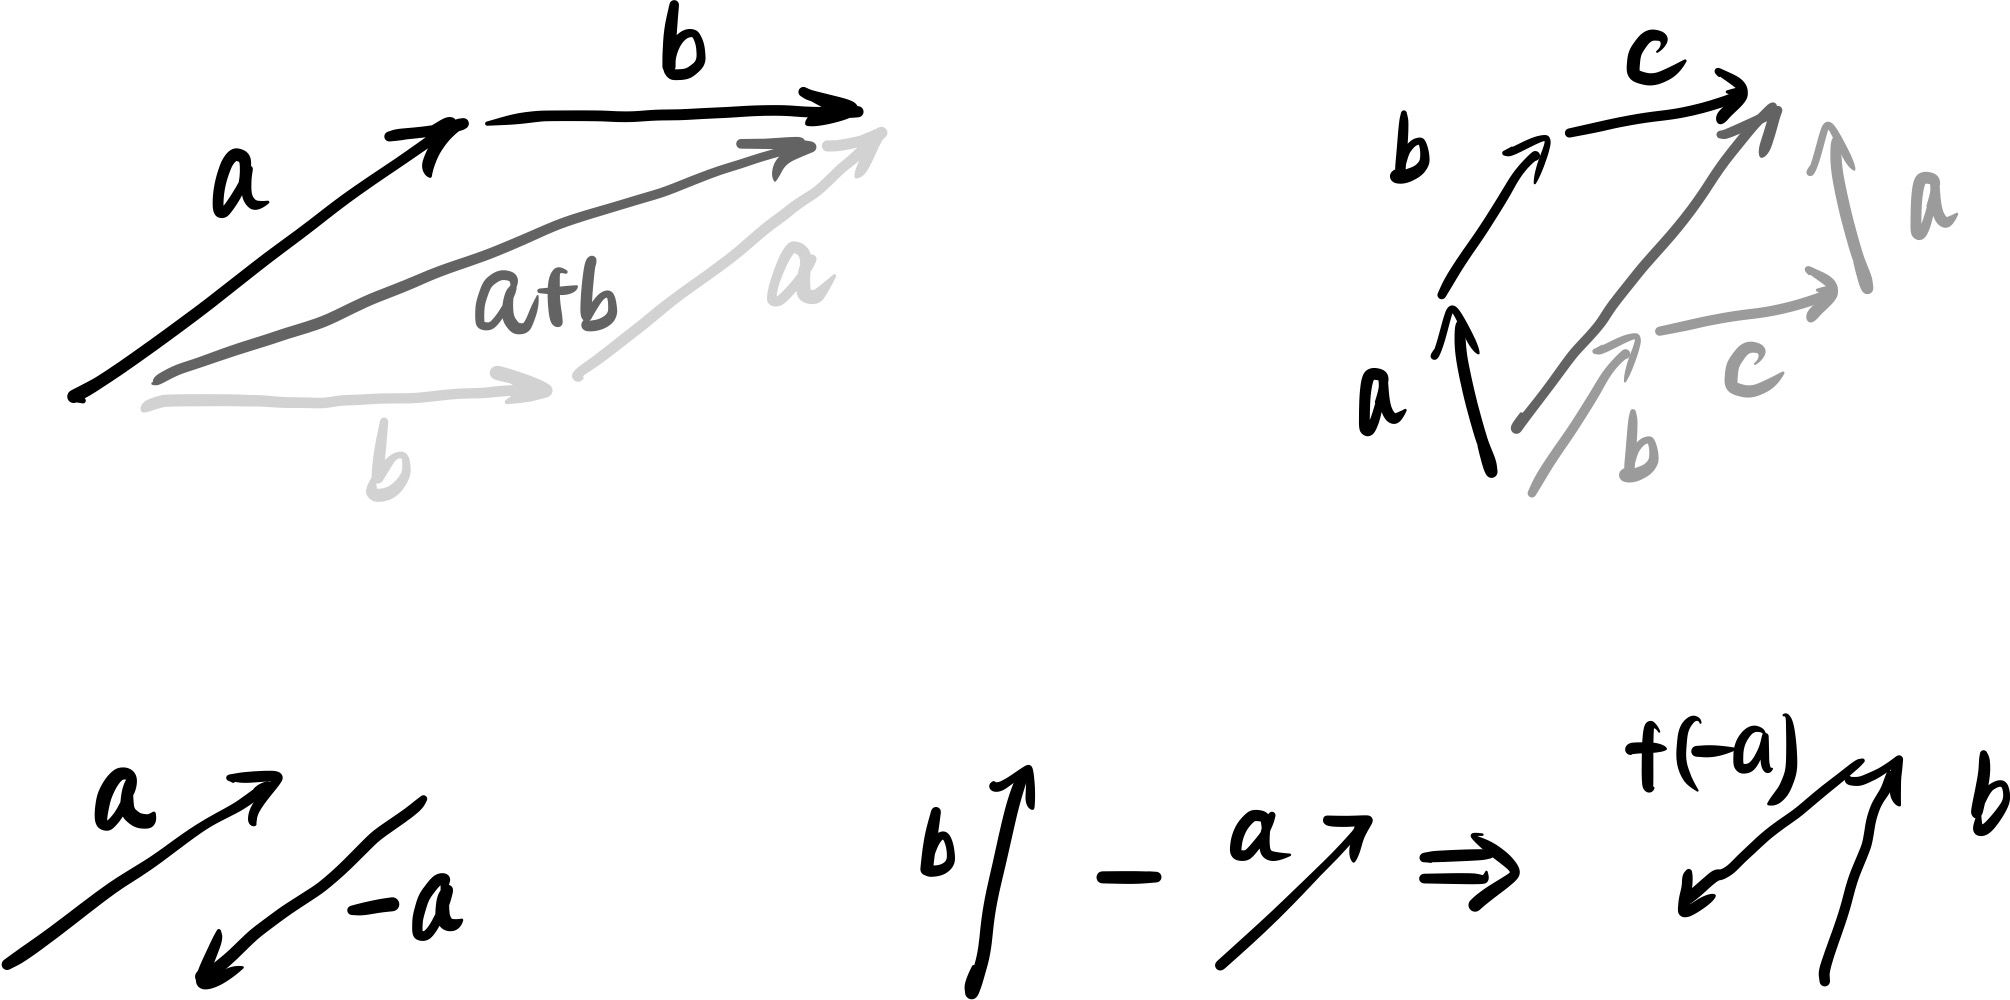
\includegraphics[width=0.8\textwidth]{img/image-20231128153431774.png}
\end{tcolorbox}

数乘则可看作被箭头被``放大''的倍数:

\begin{tcolorbox}[size=fbox, breakable, enhanced jigsaw]
  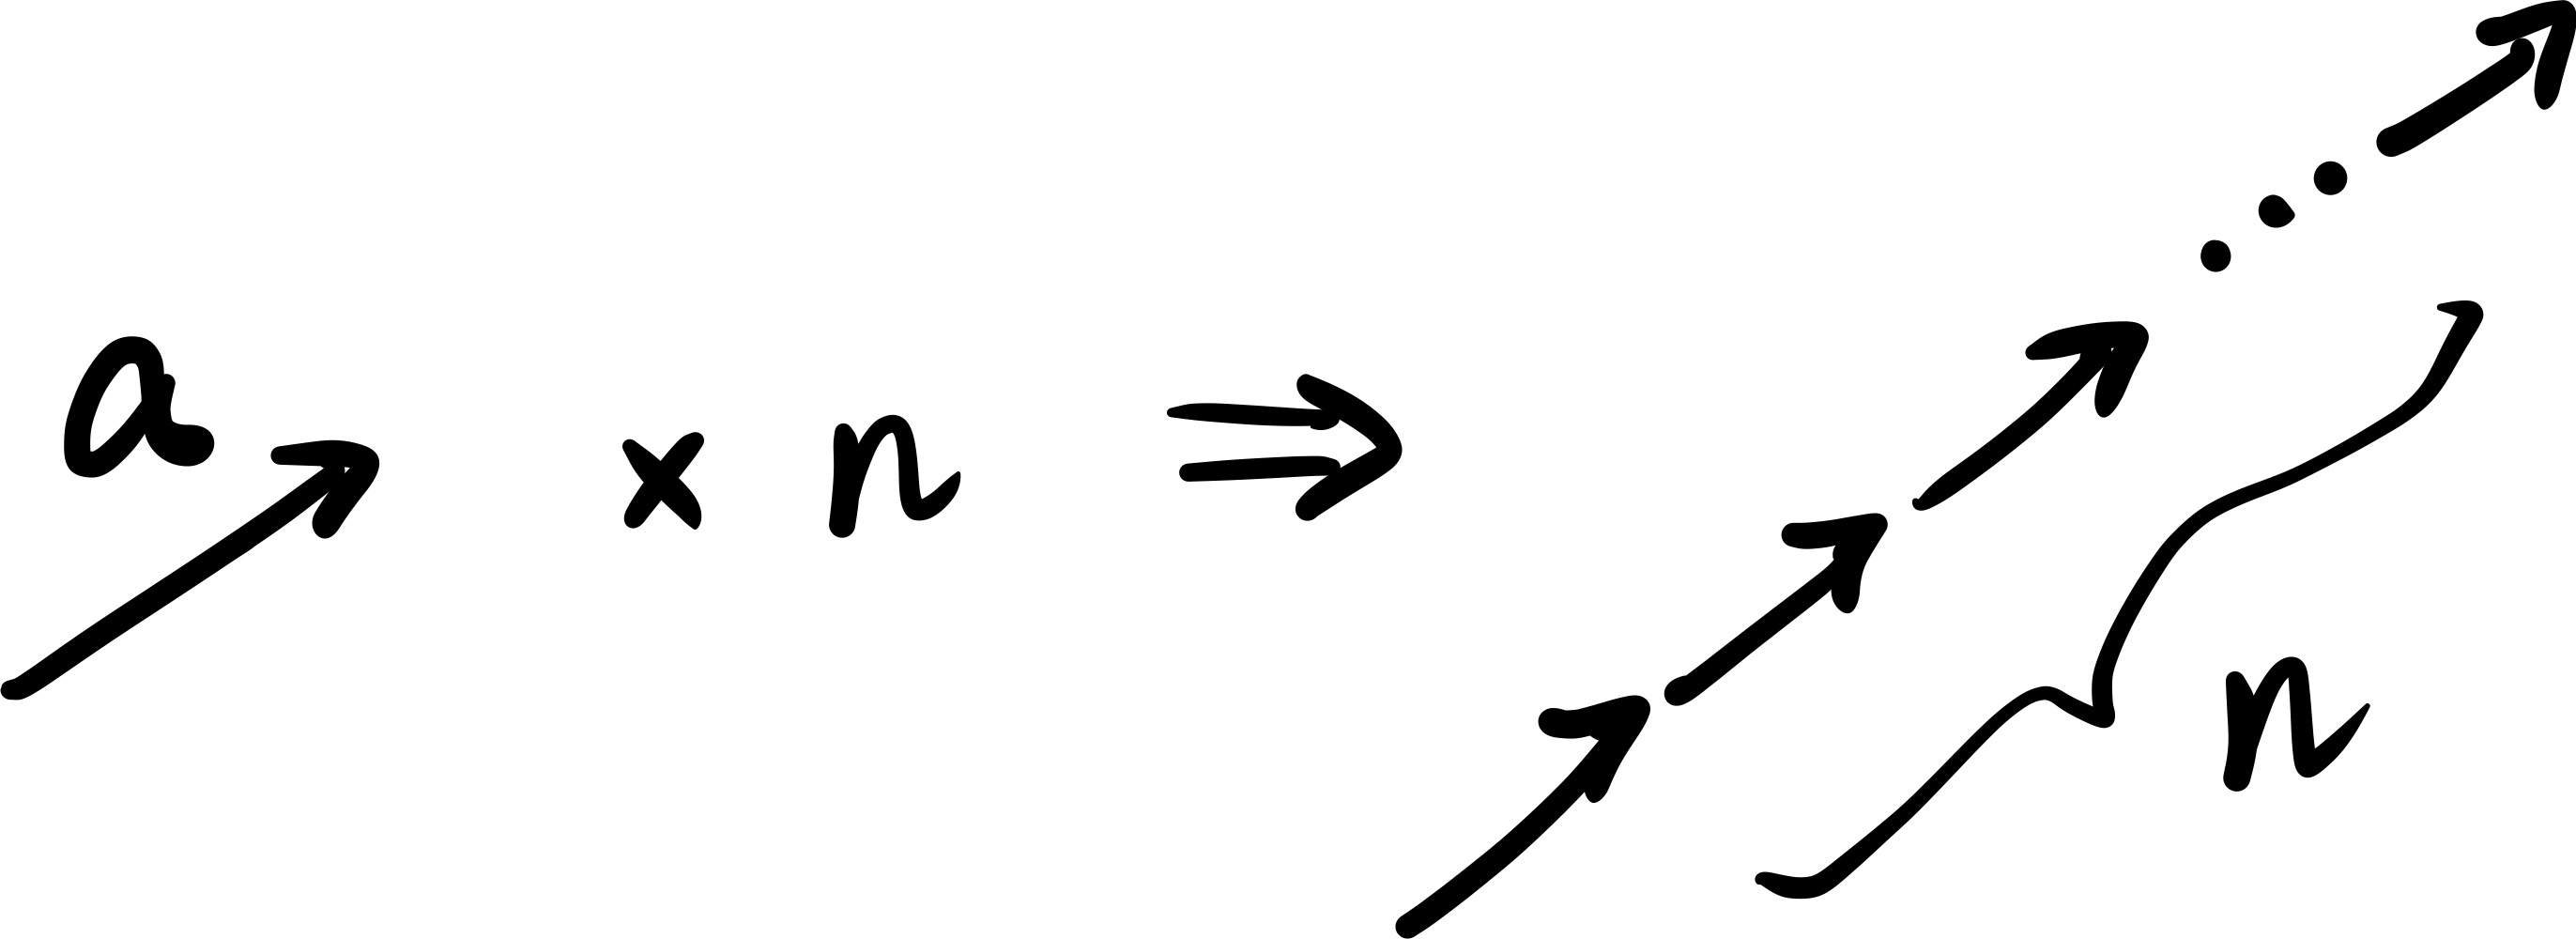
\includegraphics[width=0.4\textwidth]{img/image-20231128154149363.png}
\end{tcolorbox}

更``接地气''一点, 我们回到我们的欧氏空间, 考虑三维的情况, 将平行于
$x-$, $y-$, 和 $z-$轴的单位向量分别记作 $\hat{\imath}$,
$\hat{\jmath}$, and $\hat{k}$,

\begin{newquote}
当然很多教材也会用 $\{\hat{x},\hat{y},\hat{z}\}$ 或者
$\{\hat{e}_1,\hat{e}_2,\hat{e}_3\}$ 等等标记,
符号上的尖尖英语中一般叫做 hat - 帽子, 来强调它们是单位向量,
即``长度''为1 (其实到目前为止还并没有定义长度这个概念).

另外要注意一点, 学习的时候不应该太拘泥于符号的统一,
而应该去理解符号背后到底要表达什么. 阅读的时候,
可以理解作者要表达的就足矣, 不要因为标记和自己习惯的不同而不悦,
但自己整理知识点, 消化的时, 有一套相对统一的标记还是会比较方便.
\end{newquote}

这样一来一个三维欧式空间 $\mathbb{R}^3$
里的一个向量就可以用分量形式来表示了, 就像 \[
\boldsymbol{a}=a_x\hat{\imath}+a_y\hat{\jmath}+a_z\hat{k}.
\] 这里 $a_x$, $a_y$, 和 $a_z$ 分别是向量 $\boldsymbol{a}$ 在
$x-$, $y-$, 和 $z-$轴方向上的分量, 或者说投影 (如下图所示).

\begin{tcolorbox}[size=fbox, breakable, enhanced jigsaw]
  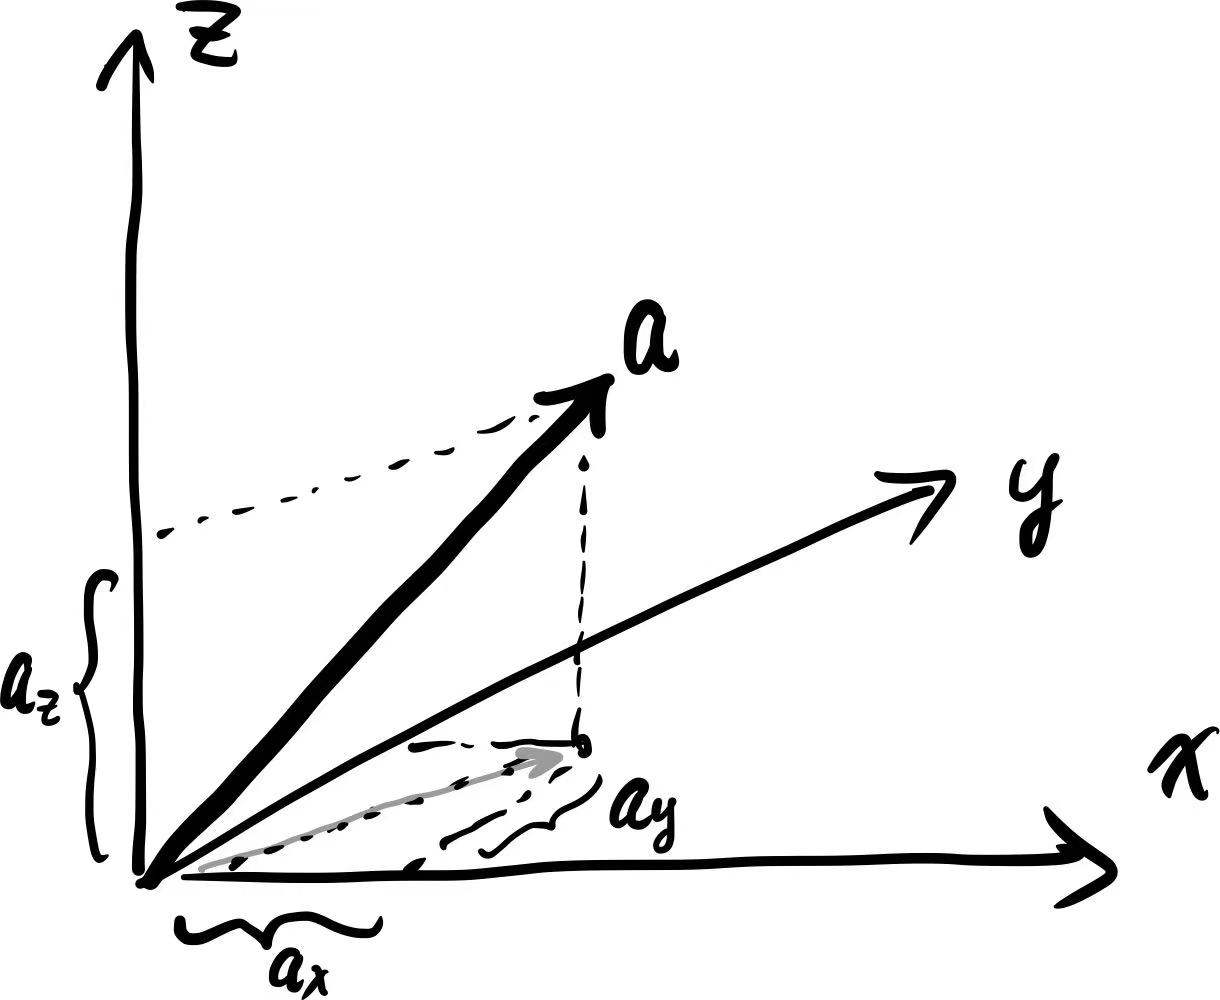
\includegraphics[width=0.4\textwidth]{img/image-20231128170037975.png}
\end{tcolorbox}

除此之外, 也可以理解成, 向量 $\boldsymbol{a}$ 是 $a_x\hat{\imath}$,
$a_y\hat{\jmath}$, 和 $a_z\hat{k}$ 这三个向量的和.

利用分量形式, 还可以更直观得表述 (注意不是证明) 前面的八条性质. 考虑
$\boldsymbol{a}=a_x\hat{\imath}+a_y\hat{\jmath}+a_z\hat{k}$ 和
$\boldsymbol{b}=b_x\hat{\imath}+b_y\hat{\jmath}+b_z\hat{k}$,
加法交换律便可写作 \[
\begin{aligned}
\boldsymbol{a}+\boldsymbol{b}&=a_x\hat{\imath}+a_y\hat{\jmath}+a_z\hat{k}+b_x\hat{\imath}+b_y\hat{\jmath}+b_z\hat{k}\\
&=(a_x+b_x)\hat{\imath}+(a_y+b_y)\hat{\jmath}+(a_z+b_z)\hat{k}\\
&=(b_x+a_x)\hat{\imath}+(b_y+a_y)\hat{\jmath}+(b_z+a_z)\hat{k}=\boldsymbol{b}+\boldsymbol{a}.
\end{aligned}
\] 可以观察到, 在进行向量计算时, 我们可以对各分量进行运算,
而分量的运算则是完全符合一个数域的性质的.

\begin{newquote}
笔者本人最早是在高中自学一些力学题时, 比较系统地接触向量的,
因为高中大多数力学题会把力或是运动分解到正交 (垂直) 的方向上进行分析,
所以事实上是没有必要利用向量来计算的,
仅仅计算各个方向上的分量就足以解决几乎所有问题,
于是当时一直很疑惑引入向量的目的.

后面随着学习的深入, 特别是本科阶段接触到了向量微积分后,
才意识到使用向量带来标记上的方便; 再后面学到了量子力学后, 接触了 bra-ket
(即左矢右矢), 或者说 Dirac notation (狄拉克符号), 更是意识到,
把向量视作一个抽象的对象, 而不是展开成一个具体的形如分量乘以基底, 即
$\boldsymbol{a}=\sum a_i\hat{e}_i$ 的优势; 一方面来讲,
基底的选择是比较任意的 (大多数时候, 只要完备正交归一就是``好''的,
然后怎么方便怎么来. \textless 什么是正交归一? 先挖个坑\textgreater);
另一方面来说, 把向量看作一个抽象的对象更方便去关注它本身的一些性质,
而不会被它在某个基底下的展开束缚和梏桎住想法.
\end{newquote}

\section{点乘}\label{025}

前面我们看到向量有数乘这个运算, 那么向量之间有类似乘法得运算吗?

Well, 还是先从熟悉的三维欧氏空间 $\mathbb{R}^3$ 出发, 遂有单位向量
$\hat{\imath}$, $\hat{\jmath}$, 和 $\hat{k}$. 不难看出,
三维欧式空间里任意的一个向量, 都可以用这三个单位向量的倍数之和来表示,
于是在这样的上下文下 (under this context),
这三个单位向量可以被称为\textbf{基}或\textbf{基底} (basis),
它们\textbf{张成} (span) 了 $\mathbb{R}^3$ 中的全体向量的集合.

\begin{newquote}
当然这个基底的选择并不是唯一的. 一个``好的", 合理的选择应该满足:

首先是\textbf{基向量} (basis vector) 的数量,
基向量的数量应该和维度是一致的, 否则自由度会不够; 就 $\mathbb{R}^3$
为例, 如果只选取两个向量作为基向量, 它们所有的\textbf{线性组合} (linear
combination), 即它们两个的倍数之和, 被限制在了一个平面里,
而无法``覆盖''整个三维立体的空间.

还有是, 基向量之间应该是\textbf{线性不相关} (linearly
independent) 的,
即其任意一个基向量不应该能被剩余的其他基向量的线性组合表示; 还是考虑
$\mathbb{R}^3$ 中的情况, 两个基向量的线性组合已经``覆盖''了一个平面,
若第三个基向量的选取是前两个基向量的线性组合, 那么它依旧在那个平面内,
从而使得这三个向量的线性组合无法覆盖整个三维立体的空间.

举一个更具体地例子,
$\{\frac{\hat{\imath}+\hat{\jmath}}{\sqrt{2}},\frac{-\hat{\imath}+\hat{\jmath}}{\sqrt{2}},\hat{k}\}$,
也就是原先的三个基向量, 以 $z-$轴为旋转轴,
顺时针旋转45°得到的三个新的向量, 也可以是一组基底.

当然, 基向量的数量也可以多于维数, 基向量间也可以是线性相关的, 这样就有一定的冗余度, 一个向量在这样的基底展开下可以有多种形式, 没有唯一的展开形式在很多场合下就不够``好".
\end{newquote}

在 $\{\hat{\imath},\hat{\jmath},\hat{k}\}$ 这个基底选择下, 我们定义``点乘'' ((dot product)) 这个向量乘法, 点乘规律可以总结为: 对于向量
$\boldsymbol{a}=a_x\hat{\imath}+a_y\hat{\jmath}+a_z\hat{k}$ 和
$\boldsymbol{b}=b_x\hat{\imath}+b_y\hat{\jmath}+b_z\hat{k}$,
它们的点乘是 \[
\boxed{\boldsymbol{a}\cdot\boldsymbol{b}=a_xb_x+a_yb_y+a_zb_z}.
\] 这是因为我们规定, \[
\begin{cases}
\hat{\imath}\cdot\hat{\imath}=1\\
\hat{\jmath}\cdot\hat{\jmath}=1\\
\hat{k}\cdot\hat{k}=1
\end{cases},
\begin{cases}
\hat{\imath}\cdot\hat{\jmath}=\hat{\jmath}\cdot\hat{\imath}=0\\
\hat{\imath}\cdot\hat{k}=\hat{k}\cdot\hat{\imath}=0\\
\hat{\jmath}\cdot\hat{k}=\hat{k}\cdot\hat{\jmath}=0
\end{cases}.
\] 于是某种意义上, 点乘可以看作正常的乘法, 即: 
\begin{align*}
\boldsymbol{a}\cdot\boldsymbol{b}=&(a_x\hat{\imath}+a_y\hat{\jmath}+a_z\hat{k})(b_x\hat{\imath}+b_y\hat{\jmath}+b_z\hat{k})\\
=&a_x\hat{\imath}(b_x\hat{\imath}+{b_y\hat{\jmath}+b_z\hat{k}})\\
&+a_y\hat{\jmath}({b_x\hat{\imath}}+b_y\hat{\jmath}+{b_z\hat{k}})\\
&+a_z\hat{k}({b_x\hat{\imath}+b_y\hat{\jmath}}+b_z\hat{k}).
\end{align*}

写成分量形式后可以看出, 点乘这个运算是有交换律和结合律的.

\begin{newquote}
\textbf{正交归一基}/\textbf{正交规范基} (orthonormal basis)
$\{\hat{\imath},\hat{\jmath},\hat{k}\}$ 这个基底选择带来的一个好处是,
基向量之间的乘法非常容易总结: 不同的基向量相乘得到 $0$ - 正交,
同样的基向量相乘得到 $1$ - 归一 ; 更通常的, 如果有一组正交归一基,
$\{\hat{e}_1,\hat{e}_2,\hat{e}_3,…\}$, 基向量之间的乘法可以利用
Kronecker Delta表述为 \[
\hat{e}_i\hat{e}_j=\delta_{ij}=\begin{cases}1\ \text{if }i=j\\0\ \text{if }i\neq j\end{cases}.
\] 在 $\mathbb{R}^3$ 中, 正交可以比较肤浅的理解成两向量是垂直的,
而归一则可以理解为向量的``长度''是 $1$ (again
事实上我们还没有定义距离, but soon enough
我们就可以有``距离''这个概念了).

虽然正交归一是一个很好的性质, 但是基底的选择未必需要正交归一性; 当我们有一组比较任意的线性无关向量时, 若我们需要一组正交归一的基向量, 我们可以通过施密特正交化 (Schmidt orthogonalization) 来得到, 具体的过程这里就不做展开了.
\end{newquote}

\subsubsection{内积 (inner product, 选读)}

严格点来说, 点乘是一种内积, 或者也可以说, 内积是点乘的推广.

在\ref{024}\nameref{024}中, 我们看到, 向量这个概念事实上比我们想象得要更宽泛一些,
例如所有的光滑函数 $C^\infty$ 可以视作一个线性空间,
不难发现函数加法和函数数乘这两个运算是满足封闭性的,
同时余下的八条运算规律也是满足的.

至于基底的选择, 可以是多项式, 在\ref{016}\nameref{016}中,
【对一个函数做泰勒展开】就好比【向量写作分量形式】, \[
f(x)=\sum_{n=0}^\infty\frac{f^{(n)}(x_0)}{n!}(x-x_0)^n.
\] $(x-x_0)^n$ 和 $\frac{f^{(n)}(x_0)}{n!} $
相当于基向量和各基向量对应的分量, 值得注意的一点是, 在这个例子中,
基向量的数量是无限多的, 即所有连续函数构成的线性空间是无限维的.

除了多项式以为, 三角函数也是一个很好的选择, 忽略亿点点细节, 在一个区间
$[-\pi,\pi]$ 里一个函数的\textbf{傅立叶级数} (Fourier series) 可以写作
\[
f(x)=\frac{a_0}{2}+\sum_{n=1}^\infty\left(a_1\cos(nx)+b_n\sin(nx)\right),
\] 其中 \[
\begin{aligned}
a_n=\frac{1}{\pi}\int_{-\pi}^\pi f(x)\cos(nx)\mathrm{d}x,\\
b_n=\frac{1}{\pi}\int_{-\pi}^\pi f(x)\sin(nx)\mathrm{d}x.
\end{aligned}
\]

并且 $n$ 为正整数. 注意到 \[
\begin{aligned}
&\frac{1}{\pi}\int_{-\pi}^{\pi}\cos(nx)\cos(kx)\mathrm{d}x=\delta_{kn},\\
&\frac{1}{\pi}\int_{-\pi}^{\pi}\sin(nx)\sin(kx)\mathrm{d}x=\delta_{kn},\\
&\frac{1}{\pi}\int _{-\pi}^{\pi}\cos(nx)\sin(kx)\mathrm{d}x=0.
\end{aligned}
\] 也就是说, 如果我们把积分 $\int f(x)g(x)\mathrm{d}x$, 视作函数
$f(x)$ 和 $g(x)$ 的内积 (在这个例子里, 积分前还需要加一个归一化系数
$\frac{1}{\pi}$), 那么基底 $\{\cos(nx),\sin(nx)\}$ 便是正交归一的.

\begin{newquote}
上述的情况都是对于变量是实数的函数, 即实变函数 (functions of a real
variable), 将内积的概念推广到复变函数 (functions of a complex variable)
便成了 Hermitian 内积, $f(z)$ 和 $g(z)$ 的内积会是形如
$\int\bar{f}(z)g(z)\mathrm{d}z$, 上加一杠表示求复共轭 (参见\ref{006}\nameref{006}).

类似的, 对于分量含有复数的``通常''的向量, Hermitian 内积也应形如
$\bar{\boldsymbol{a}}\boldsymbol{b}$.
\end{newquote}

另外注意到, 在求每一个基向量前的系数, 也就是求各分量 $a_n$ 和 $b_n$
的方法, 和 $\mathbb{R}^3$
中求``通常``的向量的分量的方法是几乎``一致''的: \[
a_x=\boldsymbol{a}\cdot\hat{\imath}\Leftrightarrow a_n=\frac{1}{\pi}\int_{-\pi}^\pi f(x)\cos(nx)\mathrm{d}x.
\]

\begin{newquote}
抽象化一点, 借用物理的狄拉克记号 (Dirac notation) 或者说 bra-ket
notation: 如果有一系列的向量 $\left|\psi\right>$,
$\left|\phi\right>$, \ldots; $\left|\psi\right>$ 和
$\left|\phi\right>$ 内积记作 $\left<\psi\right.\left|\phi\right>$,
若有\textbf{完备} (complete) 正交归一基
$\{\left|\hat{e}_1\right>,\left|\hat{e}_2\right>,\left|\hat{e}_3\right>,...\}$,
那么向量 $\left|\psi\right>$ 可以展开成
$\left|\psi\right>=a_1\left|\hat{e}_1\right>+a_2\left|\hat{e}_2\right>+a_3\left|\hat{e}_3\right>+...$
; 在某个基向量 $\left|\hat{e}_i\right>$ ``方向''上的分量 $a_i$
一般都可以通过 $\left<\hat{e}_i\right.\left|\psi\right>$ 来计算.

(超纲) 证明: 这里需要用到完备正交归一基的特性
$\sum_i\left|\hat{e_i}\right>\left<\hat{e}_i\right|=\hat{I}$, 这里
$\hat{I}$ 是一个单位算符 (identity operator), 相当于一,
即``什么都不做'', 于是 \[
\left|\psi\right>=\sum_i\left|\hat{e_i}\right>\left<\hat{e}_i\right.\left|\psi\right>.
\] 利用运算的结合律, 后两项的运算相当于一个内积, 运算的结果是一个标量,
于是可以向前挪, 便有 \[
\left|\psi\right>=\sum_i\left<\hat{e}_i\right.\left|\psi\right>\left|\hat{e_i}\right>,
\] 对比 \[
\left|\psi\right>=\sum_ia_i\left|\hat{e_i}\right>,
\] 便有 $a_i=\left<\hat{e}_i\right.\left|\psi\right>$.
\end{newquote}

\section{点乘(续)}\label{026}

前面比较介绍了在欧式空间里点乘的规律, 进一步地, 通过抽象化点乘这个概念,
引出了内积. 现在我们来看看两个向量的点乘到底意味着什么, 有什么用.

首先是结论: \[
\boxed{\boldsymbol{a}\cdot\boldsymbol{b}=|\boldsymbol{a}||\boldsymbol{b}|\cos\theta}.
\]

\begin{newquote}
上式中的 \(\theta\) 表示向量 \(\boldsymbol{a}\) 和 \(\boldsymbol{b}\)
之间的夹角. 等式右边的``绝对值''作用在向量上, 表示的是求向量的``大小'':
专业点说叫做``\textbf{模}'' (module); 事实上这也对应着, \(L_2\)
\textbf{范数}或者说欧氏\textbf{范数} (\(L_2\)/Euclidean norm);
理工科上也常直呼 magnitude. 很多教材也会用双竖线 \(||\cdot||\)
来标记模和范数, 用以和绝对值区分.

在三维欧式空间中, 对于
\(\boldsymbol{a}=a_x\hat{\imath}+a_y\hat{\jmath}+a_z\hat{k}\),
\(|\boldsymbol{a}|\equiv\sqrt{\boldsymbol{a}\cdot\boldsymbol{a}}=\sqrt{a_x^2+a_y^2+a_z^2}\).
\end{newquote}

上面的结论可以用余弦定律 (参见【\ref{005}\nameref{005}】) 来推导:

\begin{tcolorbox}[size=fbox, breakable, enhanced jigsaw]
  % \includegraphics[width=0.4\textwidth]{img/image-20231218163322717.png}
\end{tcolorbox}

\begin{newquote}
证明: 利用余弦定律有 \[
|\boldsymbol{a}|^2+|\boldsymbol{b}|^2-2|\boldsymbol{a}||\boldsymbol{b}|\cos\theta=|\boldsymbol{b}-\boldsymbol{a}|^2
\] 对等式右边展开有:
\(|\boldsymbol{b}-\boldsymbol{a}|^2=|\boldsymbol{a}|^2+|\boldsymbol{b}|^2-2\boldsymbol{a}\cdot\boldsymbol{b}\),
和完全平方的展开非常类似 (这一结论可以从分量的运算看出),
不过交叉项严格来说
\(-\boldsymbol{a}\cdot\boldsymbol{b}-\boldsymbol{b}\cdot\boldsymbol{a}\),
只因\footnote{只因你太美, baby.}点乘满足交换律,
于是两个交叉项事实上没有区别
(不难从【\ref{025}\nameref{025}】中发现点乘是满足交换律和结合律的). 于是 \[
|\boldsymbol{a}|^2+|\boldsymbol{b}|^2-2|\boldsymbol{a}||\boldsymbol{b}|\cos\theta=|\boldsymbol{a}|^2-|\boldsymbol{b}|^2-2\boldsymbol{a}\cdot\boldsymbol{b},
\] 遂得到结论.
\end{newquote}

这样一来, 点乘的一个应用便是找到两个向量之间的夹角. 利用这个夹角,
便可以求得一个向量在另一个向量方向上的``投影'' (projection)\footnote{``投影''其实说得很``物理'',
  考虑上文附图中, 光线沿着垂直于b的方向照在a上, 然后在b上 cast
  了一个阴影, 阴影的长度就叫a在b方向上的投影.}:

  \begin{tcolorbox}[size=fbox, breakable, enhanced jigsaw]
    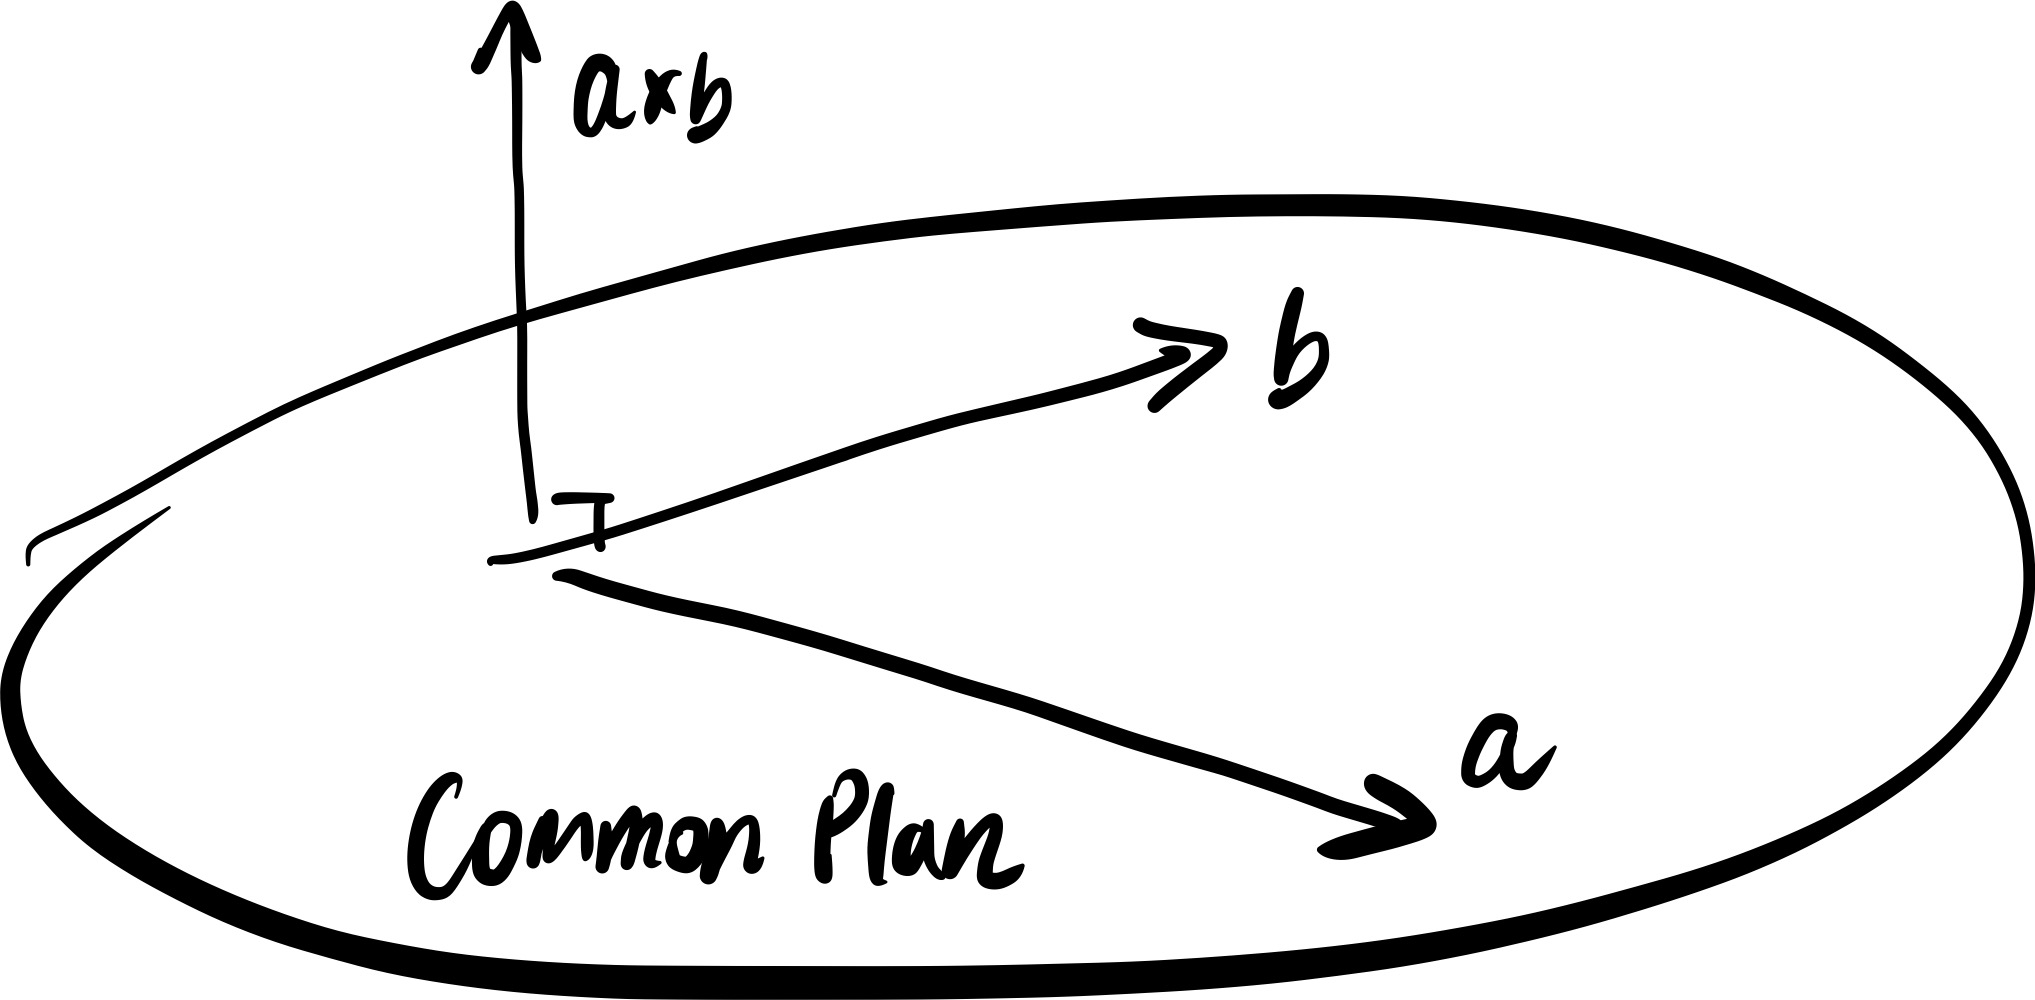
\includegraphics[width=0.4\textwidth]{img/image-20240104090927918.png}
  \end{tcolorbox}

如上图所示, \(\boldsymbol{a}\) 和 \(\boldsymbol{b}\) 的夹角 \(\theta\)
的余弦利用点乘可得是
\(\frac{\boldsymbol{a}\cdot\boldsymbol{b}}{|\boldsymbol{a}||\boldsymbol{b}|}\),
于是 \(\boldsymbol{a}\) 在 \(\boldsymbol{b}\) 方向上``投影''的长度是
\(|\boldsymbol{a}|\cos\theta=|\boldsymbol{a}|\frac{\boldsymbol{a}\cdot\boldsymbol{b}}{|\boldsymbol{a}||\boldsymbol{b}|}=\frac{\boldsymbol{a}\cdot\boldsymbol{b}}{|\boldsymbol{b}|}\),
``投影''这个向量还需要加上方向的信息, 于是有
\[
\mathrm{proj}_{\boldsymbol{b}}(\boldsymbol{a})=\frac{\boldsymbol{a}\cdot\boldsymbol{b}}{|\boldsymbol{b}|}\frac{\boldsymbol{b}}{|\boldsymbol{b}|}.
\]
很多场合下, \(\frac{\boldsymbol{b}}{|\boldsymbol{b}|}\) 这样表示向量
\(\boldsymbol{b}\) 方向上的单位向量, 经常记作 \(\hat{\boldsymbol{b}}\).


\subsubsection{叉乘}
叉乘是在三维偶氏空间 \(\mathbb{R}^3\) 中的一个特殊运算,
两个任意线性不相关的向量存在于一个公共的平面 (两条直线确定一个平面),
这样两个向量的叉乘则给出了一个垂直于这个平面的向量,
在或者说是它们共面的法向量 (normal vector) ,
再或者说同时垂直于它们二者的新的向量; 法向量的指向可以通过右手定则确定
(四指从第一个向量握向第二个向量,
拇指的指向便是这两个向量叉乘的结果的方向), 因此叉乘有反交换率,
i.e.~\(\boldsymbol{a}\times\boldsymbol{b}=-\boldsymbol{b}\times\boldsymbol{a}\).

计算上, 可以利用行列式 (determinant, 虽然还没正式介绍\ldots),
例如考虑\(\boldsymbol{a}=a_x\hat{\imath}+a_y\hat{\jmath}+a_z\hat{k}\) 和
\(\boldsymbol{b}=b_x\hat{\imath}+b_y\hat{\jmath}+b_z\hat{k}\),
它们的叉乘是 \[
\boldsymbol{a}\times\boldsymbol{b}=\begin{vmatrix}\hat{\imath}&\hat{\jmath}&\hat{k}\\a_x&a_y&a_z\\b_x&b_y&b_z\end{vmatrix},
\] 展开便是 \[
\boldsymbol{a}\times\boldsymbol{b}=(a_yb_z-a_zb_y)\hat{\imath}+(a_zb_x-a_xb_z)\hat{\jmath}+(a_xb_y-a_yb_x)\hat{k}.
\]

\begin{tcolorbox}[size=fbox, breakable, enhanced jigsaw]
  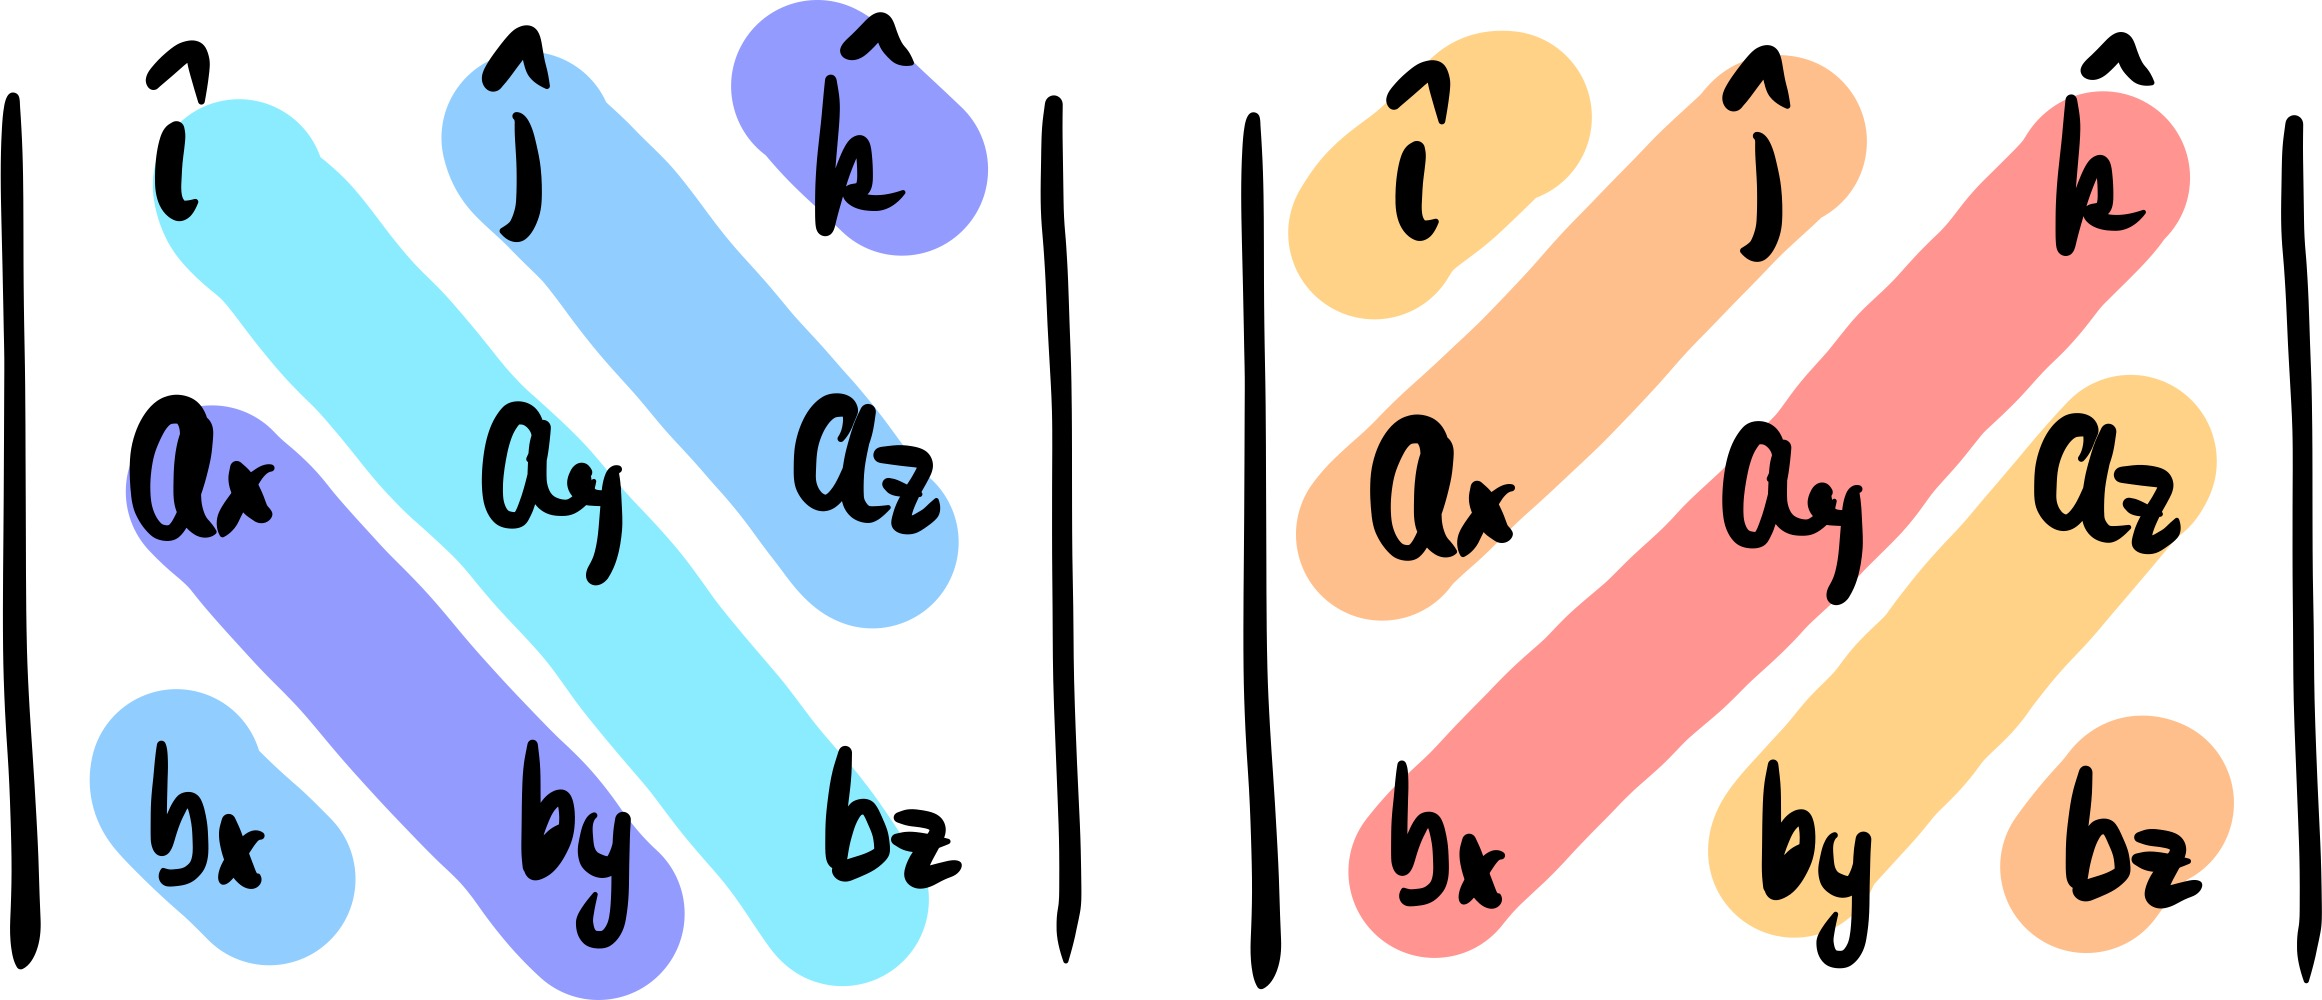
\includegraphics[width=0.4\textwidth]{img/image-20240104090600239.png}
  [size=fbox, breakable, enhanced jigsaw, sidebyside]
  \kaishu{
    个人的记忆方法是, 左上向右下的对角线之和
    (凑不够三项相乘的对称到另一边补), 减去右上向左下的对角线之和.
  }
\end{tcolorbox}

叉乘本身不能推广到更高维, 但是叉乘事实上是楔积 (wedge product)
\(\wedge\), 楔积便没有维度的限制了, 并且【\ref{021}\nameref{021}】中提到的体积元,
更严格来讲应该是类似
\(\mathrm{d}V=\mathrm{d}x\wedge\mathrm{d}y\wedge\mathrm{d}z\).

\begin{newquote}

\textbf{关于楔积, 外积, 和张量积} - 选读

楔积也叫做外积 (exterior product), 命名和``内''相对的原因: 以
\(\mathbb{R}^3\) 为例, 内积使得原来两个向量变成了一个标量,
损失了一些信息, ``缩并''\footnote{Spoiler alert: 指标缩并 (index
  contraction).}向内了;
而外积则产生了原先两个向量共面之``外''的一个向量.

【\ref{025}\nameref{025}】讨论内积的时候, 我们借用了狄拉克记号, 其中有
\(\left|\ \right>\left<\ \right|\) 这样一个操作, 因为和内积
\(\left<\ \right|\left.\right>\) 正好反过来, 于是很多时候被称为 outer
product, 并没有对应的中文 (不是外积! 不是外积! 不是外积!),
这个运算事实上是张量积.

利用行/列向量, 和矩阵乘法的规则 (左边的行乘右边的列), 考虑
$\boldsymbol{a}=\begin{pmatrix}a_x\\a_y\end{pmatrix}$,
$\boldsymbol{b}=\begin{pmatrix}b_x\\b_y\end{pmatrix}$, 内积和外积分别是

\begin{align*}
\left<{\boldsymbol{a}}\right|\left.\boldsymbol{b}\right>\Rightarrow&\boldsymbol{a}^T\boldsymbol{b}\\
=&\begin{pmatrix}a_x&a_y\end{pmatrix}\begin{pmatrix}b_x\\b_y\end{pmatrix}\\
=&a_xb_x+a_yb_y\Rightarrow\boldsymbol{a}\cdot\boldsymbol{b};
\end{align*}

\begin{align*}
\left|{\boldsymbol{a}}\right>\left<{\boldsymbol{b}}\right|\Rightarrow&\boldsymbol{a}\boldsymbol{b}^T\\
=&\begin{pmatrix}a_x\\a_y\end{pmatrix}\begin{pmatrix}b_x&b_y\end{pmatrix}\\
=&\begin{pmatrix}a_xb_x&a_xb_y\\a_yb_x&a_yb_y\end{pmatrix}\Rightarrow{\boldsymbol{a}}\otimes{\boldsymbol{b}}.
\end{align*}

可以看到 exterior product 和 outer product 区别很大, 此外非彼外.
至于左右矢为什么分别对应向量和向量的转置, 这就涉及到对偶空间 (dual
space) 了, 暂时不做展开.

\end{newquote}
\section{插曲: 距离, 范数, 和内积 -
选读}

\subsubsection{距离}

终于要填``距离''这个坑了. 虽然前面的许多论述不时用到了``距离'',
我们脑子里也都一直有``距离''这个概念, 但是事实上自这个系列开头一来,
并没有定义过距离. 正如这个系列``从零开始''一样,
我们需要``忘记''和抛弃先前的一些预有设定,
从无开始重新``发明''距离这个概念.

考虑一个空间 \(\mathbb{V}\), 把空间中的两个元素或者说两个点
\(x,y\in\mathbb{V}\) 的距离记作 \(d(x,y)\) (相当于一个函数, input
是空间中的两个元素/点, output 是一个标量). 我们希望距离应该有以下性质:

\begin{itemize}

\item
  非负性 (nonnegative): \(d(x,y)\ge0\), 距离应该是非负的;
\item
  非退化性 (nondegenerate)\footnote{物理中 degenerate
    会被翻译成``简并'', 通常指多个状态占用同一个能级; 非简并便是,
    每个能级只有一个状态了; 和这里距离为零便是同一点的``味道''就很像了.}:
  \(d(x,y)=0\) if and only if\footnote{当且仅当, 通常会简写成 iff;
    若命题A iff 命题B, 则命题A可推出命题B, 命题B亦可推出命题A,
    有时记作↔️.} \(x=y\), 两点间距离为零, 当且仅当这两点是同一点;
\item
  对称性 (symmetric): \(d(x,y)=d(y,x)\), \(x\) 到 \(y\) 的距离和 \(y\)
  到 \(x\) 的距离一致;
\item
  三角不等式 (triangular inequality): \(d(x,y)+d(y,z)\ge d(x,z)\).
\end{itemize}

这些性质在欧氏空间里是易见的,
然而``距离''未必要用``直线距离''和勾股定律来定义,
比如考虑一个只有南北走向的 street 和东西走向的 avenue 的街区,
两个位置之间行车的距离便是所谓曼哈顿距离 (Manhattan distance).

\begin{newquote}
碎碎念: 这么叫大概是因为纽约曼哈顿的城市规划使得每个街区非常方正,
道路的走向非常统一; 当然巴塞罗那在这一点做得更令强迫症一本满足.

相对论里, 时空被统一成一个整体, 于是有时会讨论两个事件之间时空上的距离,
但是时间这个维度和空间这个维度的性质又不大一样,
所以距离的定义也是非欧几里得的 (non-Euclidean). 狭义相对论里,
只讨论相对运动导致的一些现象时, 我们会使用闵可夫斯基距离 (Minkowski
distance), 具体的距离以及其他物理量的运算会涉及到度规张量 (metric
tensor), 这个有机会再展开了; 更复杂一点的,
在广义相对论里``引力''被视作时空的扭曲, 例如讨论静止黑洞附近的时空时,
还会用到施瓦西度规 (Schwarzschild metric).
\end{newquote}

定义了距离的空间便是一个度量空间 (metric space).


\subsubsection{范数}

在一个线性空间里, 我们可以定义一个范数,
一个元素的范数可以理解为这个元素到零元的距离. 一个元素 \(x\)
的范数在很多教材中记作 \(||x||\), 它需要满足:

\begin{itemize}

\item
  非负性: \(||x||\ge 0\), 范数是非负的;
\item
  非退化性: \(||x||=0\) iff \(x=0\),
  一个元素的范数为零当且仅当这个元素是它所在的线性空间中的零元.
\item
  齐次性 (homogeneity): 若有一标量 \(a\), \(||ax||=|a|\cdot||x||\);
\item
  三角不等式: \(||x+y||\le||x||+||y||\).
\end{itemize}

一个定义了范数的线性空间便是线性赋范空间 (normed linear space). 注意:
上面列出几条, 非退化性要求空间中有零元, 齐次性要求数乘封闭,
三角不等式要求加法封闭, 这便要求范数必须定义在线性空间内
(度量空间就没有这样的要求). 因为范数可以理解为一个元素和零元的距离,
换言之, 范数诱导出了距离的定义,
因此我们可以认为赋范空间也是一种度量空间.

\subsubsection{内积}

前面已经从应用的角度接触过内积 (参见【025】),
这里我们再正式且更严格的重温一遍. 大多教材会将两个元素 \(x\) 和 \(y\)
的内积记作 \(\left<x,y\right>\), 内积满足:

\begin{itemize}

\item
  非负性: \(\left<x,x\right>\ge0\), 一个元素与自己的内积是非负的;
\item
  非退化性: \(\left<x,x\right>=0\) iff \(x=0\),
  一个元素与自己的内积为零当且仅当它是零元;
\item
  共轭对称性 (conjugate symmetry):
  \(\left<y,x\right>=\overline{\left<x,y\right>}\),
  当线性空间是实线性空间时, 交换两个元素, 内积的结果应该是不变的,
  但是当线性空间是复线性空间时, 交换两个元素,
  内积的结果变为原先内积的复共轭 (上划线在这里表示复共轭,
  关于复共轭参见【006】, 原因见下).
\end{itemize}

\begin{newquote}
\textbf{对偶空间} (Dual space) - 选读

对于``通常''的向量 (就不考虑广义的那些, 比如某个区间内的全体光滑函数),
比如 \(\mathbb{R}^n\), 考虑两个向量 \[
\boldsymbol{a}=\begin{pmatrix}{a_1\\a_2\\\vdots}\end{pmatrix},\boldsymbol{b}=\begin{pmatrix}{b_1\\b_2\\\vdots}\end{pmatrix},
\] 当我们说它们的内积 \(\left<\boldsymbol{a},\boldsymbol{b}\right>\) 时,
what we actually meaning is that (我们实际上的意思是): \[
\left<\boldsymbol{a},\boldsymbol{b}\right>=\boldsymbol{a}^T\boldsymbol{b}.
\] 我们实际上是将 \(\boldsymbol{a}\) 的转置和 \(\boldsymbol{b}\)
去运算了, 于是便是一个行向量和列向量的运算,
这样就可以利用矩阵运算``规律'' - 行乘列: \[
\left<\boldsymbol{a},\boldsymbol{b}\right>=\begin{pmatrix}{a_1&a_2&\cdots}\end{pmatrix}\begin{pmatrix}{b_1\\b_2\\\vdots}\end{pmatrix}=\sum_ia_ib_i.
\] 但是既然都把 \(\boldsymbol{a}\), 转置了, \(\boldsymbol{a}^T\) 显然和
\(\boldsymbol{a}\) 不处于同一个线性空间,
实际上它存在于一个由原先的线性空间诱导出来的一个对偶空间里, 我们可以说
\(\boldsymbol{a}^T\) 是 \(\boldsymbol{a}\) 的对偶向量.

从 \(\mathbb{R}^n\) 变为 \(\mathbb{C}^n\) 时, 还是考虑两个向量 \[
\boldsymbol{a}=\begin{pmatrix}{a_1\\a_2\\\vdots}\end{pmatrix},\boldsymbol{b}=\begin{pmatrix}{b_1\\b_2\\\vdots}\end{pmatrix},
\] 但是现在 \(a_i\) 和 \(b_i\) 是复数, 这时我们一般这么定义内积: \[
\left<\boldsymbol{a},\boldsymbol{b}\right>=\boldsymbol{a}^\dagger\boldsymbol{b},
\] 这个匕首符号 \(\dagger\) (念作 dagger), 表示转置并对矩阵元做复共轭,
这个操做也叫做埃尔米特或厄米特共轭 (Hermitian conjugate).
于是展开可以写作 \[
\left<\boldsymbol{a},\boldsymbol{b}\right>=\begin{pmatrix}{a_1^*&a_2^*&\cdots}\end{pmatrix}\begin{pmatrix}{b_1\\b_2\\\vdots}\end{pmatrix}=\sum_ia_i^*b_i,
\] 这里 \(a_i^*\) 表示 \(a_i\) 的复共轭. 于是不难发现 \[
\left<\boldsymbol{b},\boldsymbol{a}\right>=\sum_ia_ib_i^*=\sum_i\overline{a_i^*b_i}=\overline{\left<\boldsymbol{a},\boldsymbol{b}\right>}.
\]
\end{newquote}

\begin{itemize}

\item
  对第二个变元线性, 对第一个变元共轭线性: 考虑线性空间的三个元素
  \(\boldsymbol{x}\), \(\boldsymbol{y}\), 和 \(\boldsymbol{z}\)
  和两个标量 \(a\) 和 \(b\), 我们有
  \(\left<a\boldsymbol{x}+b\boldsymbol{y},\boldsymbol{z}\right>=a^*\left<\boldsymbol{x},\boldsymbol{z}\right>+b^*\left<\boldsymbol{y},\boldsymbol{z}\right>\)
  以及
  \(\left<\boldsymbol{z}, a\boldsymbol{x}+b\boldsymbol{y}\right>=a\left<\boldsymbol{z},\boldsymbol{x}\right>+b\left<\boldsymbol{z},\boldsymbol{y}\right>\).
  (注意, 因为复向量内积定义不同, 可能也会出现对第二个变元共轭线性,
  对第一个变元线性).
\end{itemize}

定义了内积的线性空间便是内积空间 (inner product space).
通过内积也很好诱导出范数, 范数可以是一个元素对自身的内积的开方
\(||\boldsymbol{x}||=\sqrt{\left<\boldsymbol{x},\boldsymbol{x}\right>}\),
因此我们通常可以认为内积空间也是一种赋范空间, 进而也是一种度量空间.

\begin{newquote}
度规张量 (metric tensor) - 选读

有了内积, 对偶空间, 就可以浅谈一下讨论距离时提到的度规张量了. 考虑
\(\mathbb{R}^3\), 距离元用笛卡尔坐标可以表示为 \[
\mathrm{d}s^2=\mathrm{d}x^2+\mathrm{d}y^2+\mathrm{d}z^2,
\] 距离平方可以看作一个向量的内积, 利用矩阵乘法: \[
\mathrm{d}s^2=\begin{pmatrix}{\mathrm{d}x&\mathrm{d}y&\mathrm{d}z}\end{pmatrix}\begin{pmatrix}{\mathrm{d}x\\\mathrm{d}y\\\mathrm{d}z}\end{pmatrix},
\] 我们可以在中间插入一个非常 trivial 的单位矩阵 (identity matrix)
而不影响运算结果: \[
\mathrm{d}s^2=\begin{pmatrix}{\mathrm{d}x&\mathrm{d}y&\mathrm{d}z}\end{pmatrix}\begin{pmatrix}{1&0&0\\0&1&0\\0&0&1}\end{pmatrix}\begin{pmatrix}{\mathrm{d}x\\\mathrm{d}y\\\mathrm{d}z}\end{pmatrix},
\] 这个单位矩阵在这样的上下文中, 就可以视作是平直空间 (flat space) -
这个说法太物理了, 应该说 - 欧式三维空间中的度规张量.

我们可以做坐标系转换, 考虑球坐标系, \[
\begin{cases}
x=r\sin\theta\cos\phi\\
y=r\sin\theta\sin\phi\\
z=r\cos\theta
\end{cases}
\] 这里 \(r\) 表示和原点的距离, 与 \(z\)-轴的夹角 - 天顶角 (azimuthal
angle) 记作 \(\theta\), 与 \(x\)-轴的夹角 - 方位角 (polar angle) 记作
\(\phi\), 大致如下图所示.

\begin{newquote}
图片使用TikZ包绘制, 代码来自 Alexander Tsagkaropoulos 在 Stack Exchange
的回答
\href{https://tex.stackexchange.com/questions/159445/draw-in-cylindrical-and-\%20spherical-coordinates/159452}{Draw
in Cylindrical and Sperical Coordinates}.
\end{newquote}

利用微元之间的关系, 省略亿点计算上地细节, 可以发现这时距离元变为了
(当然也可以利用上图从纯几何的角度出发) \[
\mathrm{d}s^2=\mathrm{d}r^2+r^2\mathrm{d}\theta^2+r^2\sin^2\theta\mathrm{d}\phi^2.
\] 这时的度规张量就不那么 trivial 了 \[
\begin{pmatrix}{1&0&0\\0&r^2&0\\0&0&r^2\sin^2\theta}\end{pmatrix}.
\]

\begin{newquote}
多重积分的变元 - 跑题

提到了距离元, 忍不住提一下体积元, 【021】中有稍稍带过一下体元
\[\mathrm{d}V=\mathrm{d}x\mathrm{d}y\mathrm{d}z\], 在转换坐标系 (换元)
后, 除了利用坐标转换的关系得到微元之间的关系,
我们还可以非常简单粗暴地利用雅可比行列式 (Jacobian) 完成换元,
考虑坐标转换 \[(x,y)\rightarrow(u,v)\], 其中 \[x=g(u,v), y=h(u,v)\]
二重积分换元有 \[
\iint f(x,y)\mathrm{d}x\mathrm{d}y=\iint f(g(u,v),h(u,v))|J(u,v)|\mathrm{d}u\mathrm{d}v,
\] 上式中 \[
J(u,v)=\begin{vmatrix}\frac{\partial x}{\partial u}&\frac{\partial x}{\partial v}\\\frac{\partial x}{\partial u}&\frac{\partial x}{\partial v}\end{vmatrix},
\] 这样变量之间的偏微分关系构成的一个行列式便叫作雅可比行列式
(关于偏微分, 参见【023】, 关于三维以下的行列式计算,
参见【026】叉乘部分的讨论, 关于行列式通常的运算, 参见文末【附录】.),
更高维 (更多变量) 的情况并不难推广.

验证球坐标的体元是
\[\mathrm{d}V=r^2\sin\theta\mathrm{d}r\mathrm{d}\theta\mathrm{d}\phi\]
可以作为一个练习.
\end{newquote}
\end{newquote}

\subsubsection{完备化}

考虑一个度量空间 \[(X,d)\], \[\{x_n\}\] 是 \[X\] 中的数列 (虽然称作数列,
其实是可以理解为集合中的一系列元素, 或者空间里的一些列点), 若存在
\[x\in X\] 使得 \[\lim_{n\rightarrow\infty}d(x_n,x)=0\], 则 \[\{x_n\}\]
在 \[X\] 中收敛, 称为收敛列, 它的极限是 \[x\].

再考虑在同一个度量空间中, 若存在 \[N\ge1\] 使得对于任意 \[\epsilon>0\]
都有 \[d(x_m,x_n)<\epsilon\] for \[m,n\ge N\],
那么我们说这个数列是柯西列 (Cauchy sequence).

虽然直觉上一个数列若柯西应该收敛, 但是其实这是因为我们太熟悉欧氏空间了,
通常而言: 收敛列一定是一个柯西列, 但是柯西列不一定是一个收敛列.

完备性要求: 若有度量空间 \[(X,d)\], 若其中任意柯西列都是收敛列,
\[(X,d)\] 便是完备度量空间. 完备的线性赋范空间叫做巴拿赫空间 (Banach
space), 完备的内积空间叫做希尔伯特空间 (Hilbert space).

最后附上述这些空间的关系:

\begin{figure}
\centering
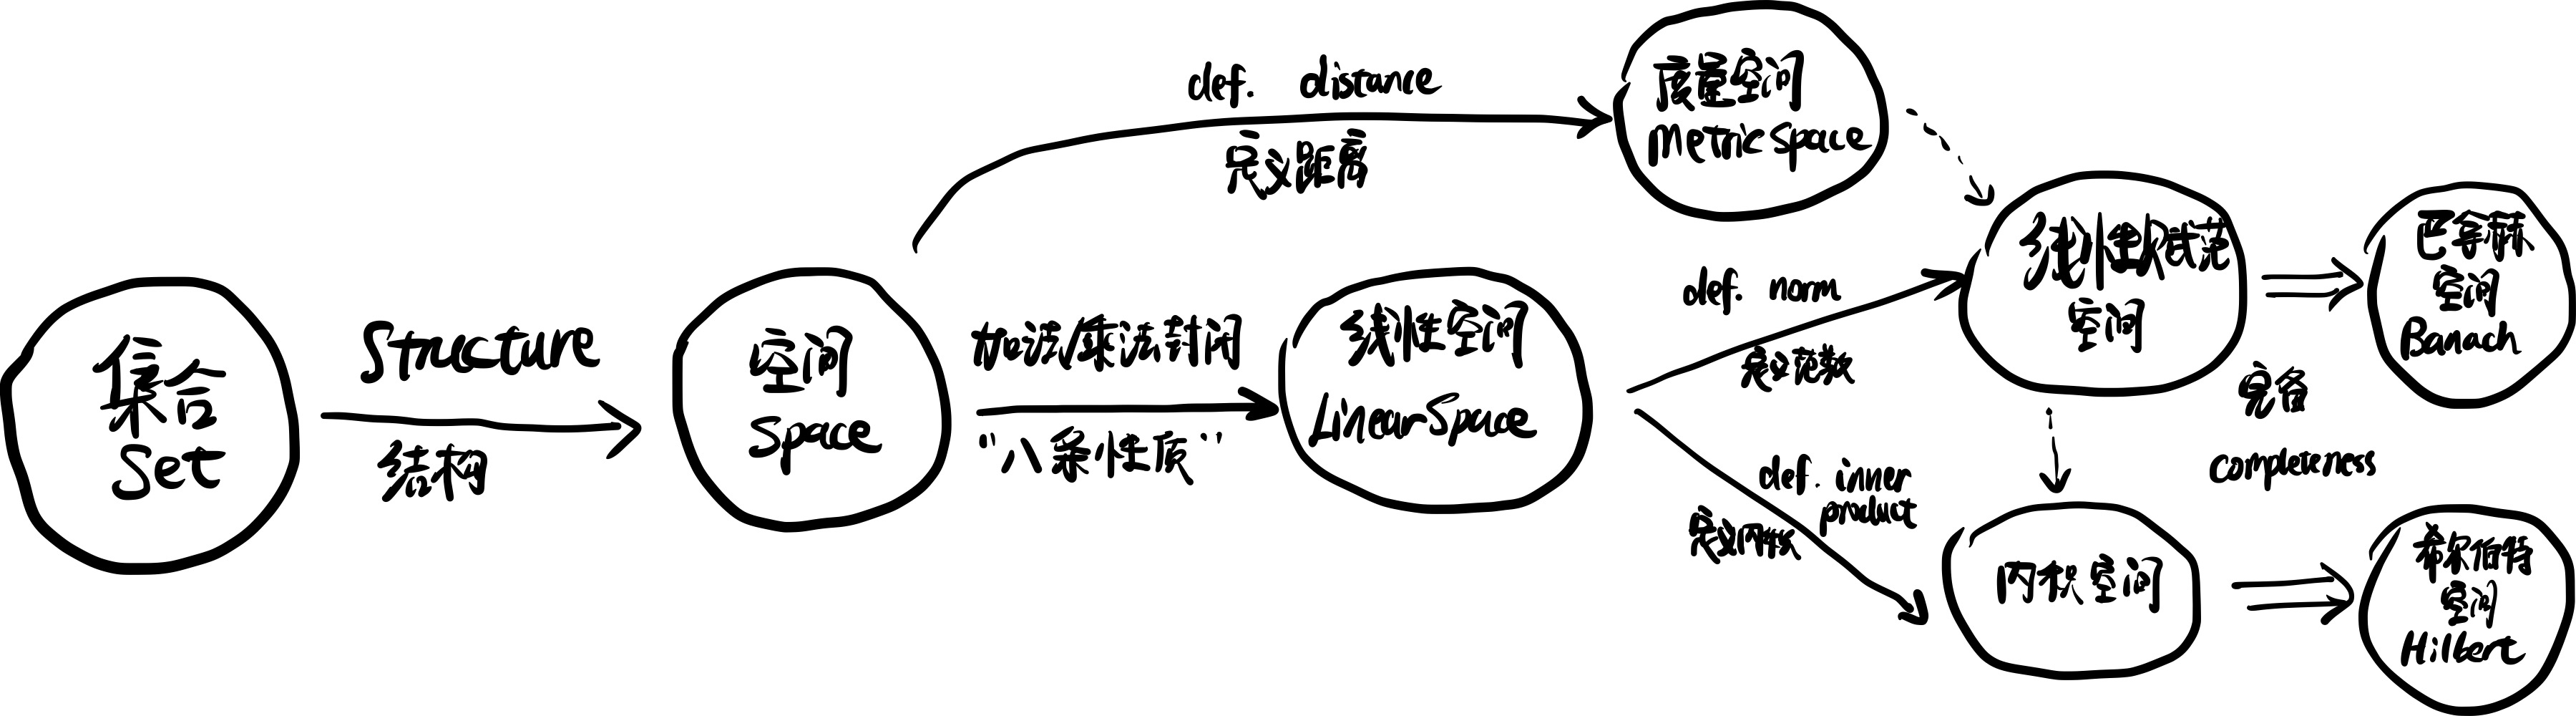
\includegraphics{C:/Users/Administrator/Documents/github/arxive/math/image-20231218171032793.png}
\caption{image-20231218171032793}
\end{figure}

\begin{newquote}
图改自知乎 @ 无尘粉笔, 本篇内容也 adapted from 他的这篇文章
\href{https://zhuanlan.zhihu.com/p/541226732}{什么是数学中的各种空间:线性空间、度量空间、赋范空间、内积空间、欧几里得空间、希尔伯特空间、巴拿赫空间?}
\end{newquote}

\subsubsection{附录:
行列式和递归}

考虑一个 \[n\times n\] 的行列式, 在计算时, 我们可以利用递归的思路:

\[n\times n\] 可以 reduce 成 \[n\] 个 \[(n-1)\times(n-1)\] 的行列式:
先把第一行第一列的元 \[a_{11}\] 拎出来,
然后计算去掉了第一行第一列的行列式, 并乘上 \[a_{11}\]; 然后把 \[a_{12}\]
拎出来, 计算去掉了第一行第二列的行列式; \ldots; 直到把 \[a_{1n}\]
拎出来, 执行类似的操作.

然后 \[(n-1)\times(n-1)\] 的行列式怎么计算呢? 出现了, 递归大法好!
我们可以将一个 \[(n-1)\times(n-1)\] 的行列式 reduce 成 \[(n-1)\] 个
\[(n-2)\times(n-2)\] 的行列式.

\ldots{}

不断重复上述操作, 直到 reduce 成许多个 \[2\times2\] 或者是 \[3\times3\]
的矩阵, 就可以用【026】提到的,
【左上向右下的对角线之和】减去【右上向左下的对角线之和】来计算了.

虽然听起来很繁琐, 但是计算大的行列式时, 这样大量重复,
但本身不复杂的运算, GPU (显卡) 最擅长了, 直接丢给计算机就可以了.
递归这种``套娃''的思路在编程中经常出现,
它和【007】中提到的归纳法其实也有一定的联系.

\section{梯度, 散度, 和旋度}\label{028}

前面我们算是过了遍向量的最基本的概念以及运算,
那么有没有关于向量的微积分呢?

\subsubsection{梯度}

考虑三维欧氏空间 \(\mathbb{R}^3\) 中的情况,
如果我们有一个多变量函数/标量场 \(f(x,y,z)\),
相当于把坐标的三个参数映射到一个标量 (暂时先只考虑实变函数):
\(\mathbb{R}^3\rightarrow\mathbb{R}\).

在【\ref{023}\nameref{023}】中, 我们发现, 多变量函数可以分别对各个变量求偏导,
而偏微分和全微分的关系是\footnote{注意, 本篇中有大量忽略函数变量的标记,
  即类似 f=f(x), 请自行脑补全缺失的部分.} \[
\mathrm{d}f=\frac{\partial f}{\partial x}\mathrm{d}x+\frac{\partial f}{\partial y}\mathrm{d}y+\frac{\partial f}{\partial z}\mathrm{d}z.
\] 令 \(\{\hat{\imath},\hat{\jmath},\hat{k}\}\)
分别为平行于三个坐标轴的单位向量, 利用它们的正交归一性,
上式可以重新写作一个点乘的形式 (复习【\ref{025}\nameref{025}】): \[
\mathrm{d}f=\left(\frac{\partial f}{\partial x}\hat{\imath}\right)\cdot\left(\mathrm{d}x\hat{\imath}\right)+\left(\frac{\partial f}{\partial y}\hat{\jmath}\right)\cdot\left(\mathrm{d}y\hat{\jmath}\right)+\left(\frac{\partial f}{\partial z}\hat{k}\right)\cdot\big(\mathrm{d}z\hat{k}\big).
\] 令 \[
\mathrm{d}\boldsymbol{r}:=\mathrm{d}x\hat{\imath}+\mathrm{d}y\hat{\jmath}+\mathrm{d}z\hat{k},
\] 即向量的线元, 再令 \[
\boxed{\nabla f:=\frac{\partial f}{\partial x}\hat{\imath}+\frac{\partial f}{\partial y}\hat{\jmath}+\frac{\partial f}{\partial z}\hat{k},}
\] 这个 \(\nabla f\) 便叫作标量场 \(f\) 的\textbf{梯度} (gradient).
于是有 \[
\mathrm{d}f=\nabla f\cdot \mathrm{d}\boldsymbol{r}.
\] 利用点乘的性质, \[
\mathrm{d}f=|\nabla f||\mathrm{d}\boldsymbol{r}|\cos\theta,
\] 其中 \(\theta\) 是梯度向量和线元向量之间的夹角. 考虑线元
\(\mathrm{d}\boldsymbol{r}\) 的大小不变但方向可以改变的情况,
在任意某一点 \((x,y,z)\) 上, 标量场的全微分 \(\mathrm{d}f\)
最大值应该发生在当 \(\theta=0\) (即\(\cos\theta=1\)),
这时线元向量和梯度向量方向一致, 或者说``沿着''梯度向量; 沿着梯度的方向,
全微分取到最大值, 意味着在这个方向上, 标量场本身变化得最快.

\begin{newquote}
于是在最优化 (optimization) 等数据科学中, 利用梯度的这一性质,
便有梯度下降法 (Gradient-Descent) 用来找局域最值 (local extrema).

其思路是: 数值 (numerical) 计算里, 有时为了计算上的便捷, 我们不求
\(|\nabla f|=0\) 的解析解; in stead, 我们知道在最值处,
就如一元微积分最值处导数为零一样, 梯度是零向量, 于是给定一个起点,
我们不断沿着梯度的方向前进, 直到梯度的大小变为零,
那么我们便到了局域的最值处.
\end{newquote}

那么 \(\nabla\) 这个符号呢, 念做 nabla, 就定义为 \[
\boxed{\nabla:=\frac{\partial}{\partial x}\hat{\imath}+\frac{\partial}{\partial y}\hat{\jmath}+\frac{\partial}{\partial z}\hat{k}.}
\] 当然, 这是在三维欧氏空间中, 使用笛卡尔坐标系时的形式, 在其他坐标系下,
它的形式会发生变化.

我们注意到, \(\nabla\) 是一个类似向量的东西, 把它作用到一个标量场后,
得到的梯度也是一个类似向量的东西.

\begin{newquote}
当然, in fact, \(\nabla\) 是一个\textbf{算子} (operator), 正如函数
(function) 可以把一个数映射到另一个数, 算子把一个函数映射到另一个函数.
下面的散度和旋度同理, 虽然运算过程中, \(\nabla\)
可以视作是一个类似向量的东西, 但是本质上它是一个算子.
\end{newquote}

\subsubsection{散度和旋度}

在讲散度之前, 先介绍一个新的概念, \textbf{向量场} (vector field). 例如,
描述空间中每一个点对应的温度的 object 叫做标量场,
描述空降中每个点对应的风速和风向的一个 object 就是 向量场了,
可以想象成空间上每一个点都有一个小箭头 (向量),
这个小箭头的大小表示风速的大小, 箭头的方向和风向一致. 这样一来,
在三维空间中的一个向量场 \(\boldsymbol{v}(x,y,z)\) 应该是一个
\(\mathbb{R}^3\rightarrow\mathbb{R}^3\) 的映射.

\begin{newquote}
现在我们可以说, 一个标量场的梯度事实上是一个向量场了.
\end{newquote}

既然标量场有类似``导数''的梯度, 向量场是不是也可以有它的``导数''呢?
应该是有的, 我们可以利用 \(\nabla\) 算子. 问题是, 现在 \(\nabla\)
也是一个类似``向量''的东西, 向量场也是一个类似``向量''的东西,
在三维空间中, 向量场作用在一个向量场有两种方法 - 点乘和叉乘,
于是这分别对应了两种向量场的``导数'' - 散度 (divergence) 和旋度 (curl).

考虑一个向量场 \[
\boldsymbol{v}(x,y,z)=v_x(x,y,z)\hat{\imath}+v_y(x,y,z)\hat{\jmath}+v_z(x,y,z)\hat{k},
\] 于是非常自然的, 有散度 \[
\boxed{\nabla\cdot\boldsymbol{v}=\frac{\partial v_x}{\partial x}+\frac{\partial v_y}{\partial y}+\frac{\partial v_z}{\partial z},}
\] 和旋度 \[
\boxed{\nabla\times\boldsymbol{v}=\begin{vmatrix}\hat{\imath}&\hat{\jmath}&\hat{k}\\\frac{\partial}{\partial x}&\frac{\partial}{\partial y}&\frac{\partial}{\partial z}\\v_x&v_y&v_z\end{vmatrix},}
\] 这里方便起见, 用了行列式的形式.

\begin{newquote}
有的教材为了记号简洁, 用类似 \(\partial_x\) 代替
\(\frac{\partial}{\partial x}\).
\end{newquote}

散度是一个标量, 因为它的运算方式和点乘类似,
它描述了在体积元内一个向量场向外的通量 (flux, 关于通量参见附录).
像下图所示的, 电场和磁场可以用向量场来描述: (i)
一个正电荷产生的电场是向外指的, 于是画一个任意的闭合曲线
(事实上应该是一个曲面, 因为画在图上方便减少了一个维度),
可以看到过这个曲面有净向外的电场线, 或者说通量是正的,
这种情况我们可以说这个曲面内有源 (source); (ii)
一个负电荷产生的电场是指向内的, 于是和前面的情况正好相反,
过一个闭合曲面有净向内的电场线, 通量是负的, 我们可以说曲面内有汇 (sink);
(iii) 磁场总是从 N 极指向 S 极, 于是画一个闭合曲面不难发现,
进入这个曲面的磁感线和出这个曲面的磁感线数量应该是一致的,
也就是说磁通量为零. 于是, 前面三个情况分别对应, 散度为正, 负, 和零.

\begin{tcolorbox}[size=fbox, breakable, enhanced jigsaw]
  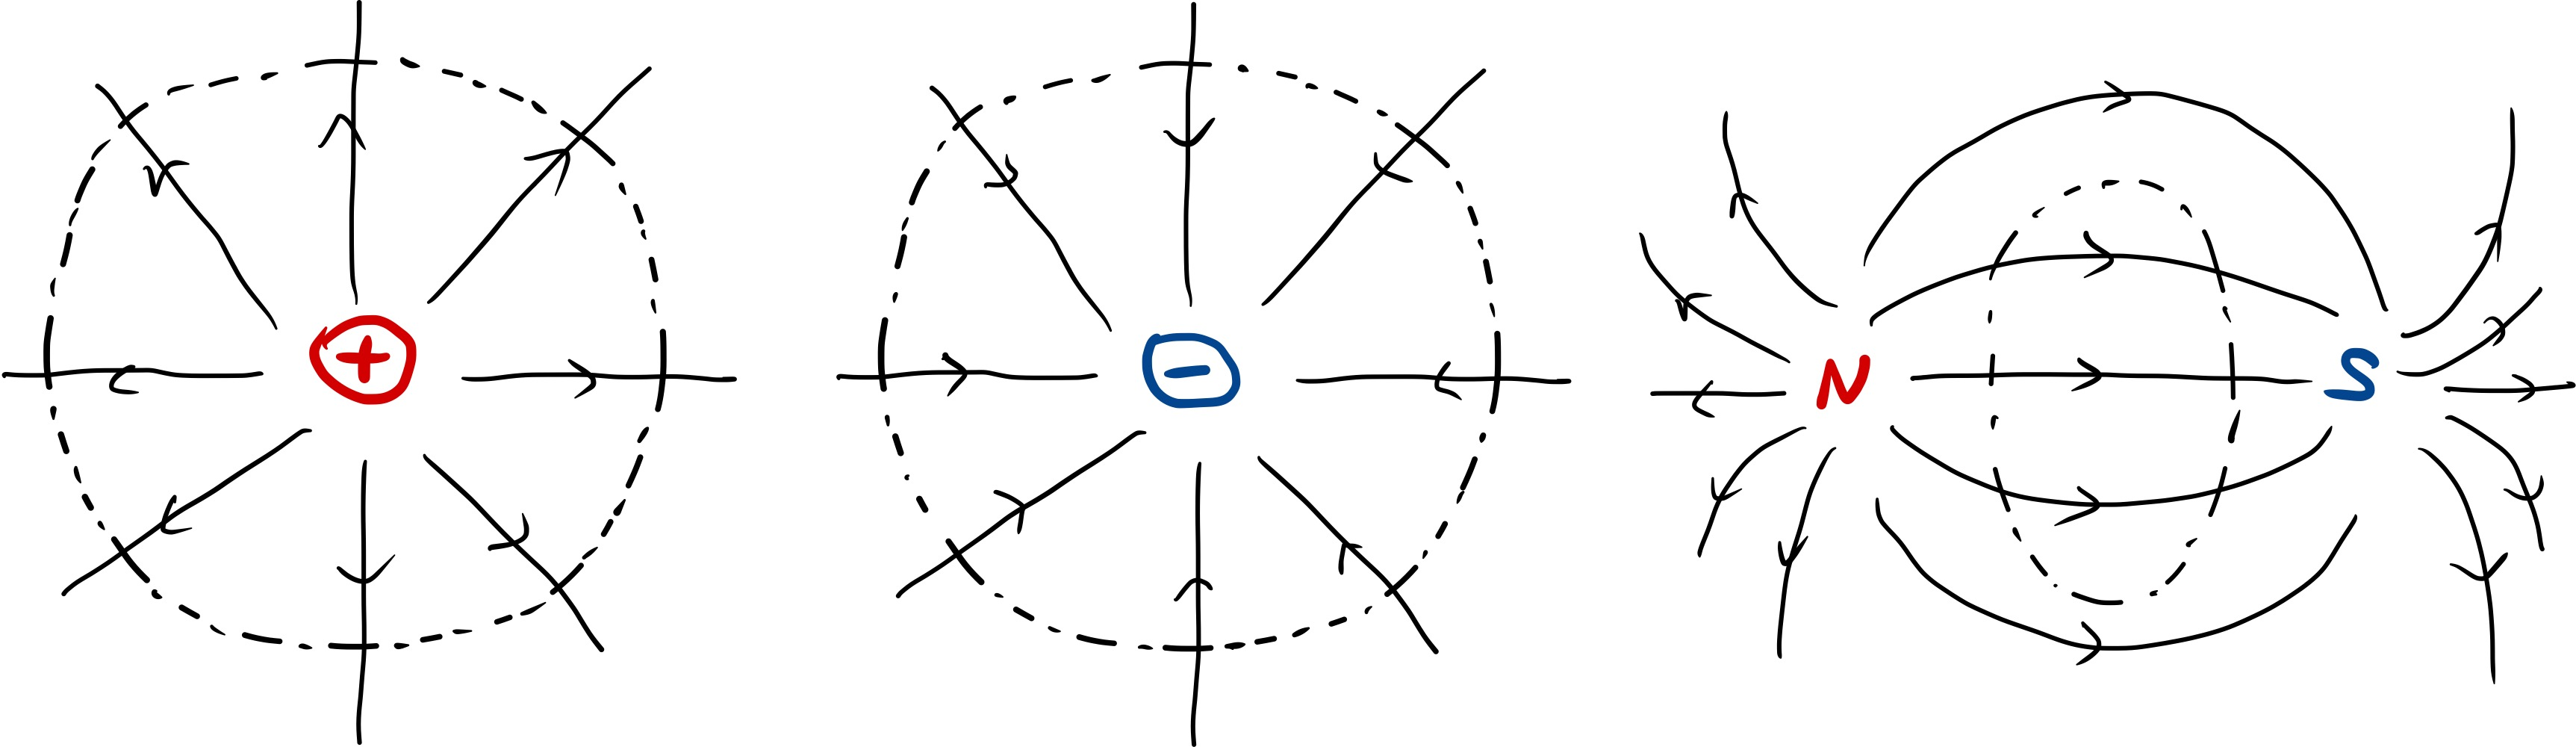
\includegraphics[width=0.9\textwidth]{img/image-20240125092014626.png}
\end{tcolorbox}

旋度是一个向量, 因为它的运算方式和叉乘类似, 它描述了每个点上的旋转.
前面这句话有那么一点抽象, 稍微落实一点, 比如向量场描述的是水流,
然后在某个点处放置一个小风车, 风车受到水流的冲击会旋转,
旋度的大小就描述了旋转的快慢, 因为旋度是一个向量,
它的指向反应了向量场旋转的方向 (如下图所示: 利用右手定则,
用四指抓握的方向表示向量场的旋转方向, 拇指的指向便是旋量的指向).

\subsubsection{附录: 通量}

首先要引入一下面积向量, 面积怎么可能用向量来表示呢? 还真可以,
两个向量的叉乘的物理意义可以是,
叉乘结果的大小反应的是它们构成的一个``平行四边形''的面积 (当然,
考虑两个向量微元的叉乘的话就是面积微元了),
叉乘结果的指向是这两个向量所在公共平面的法向 (normal), again
可以利用右手定则确定方向.

\begin{tcolorbox}[size=fbox, breakable, enhanced jigsaw]
  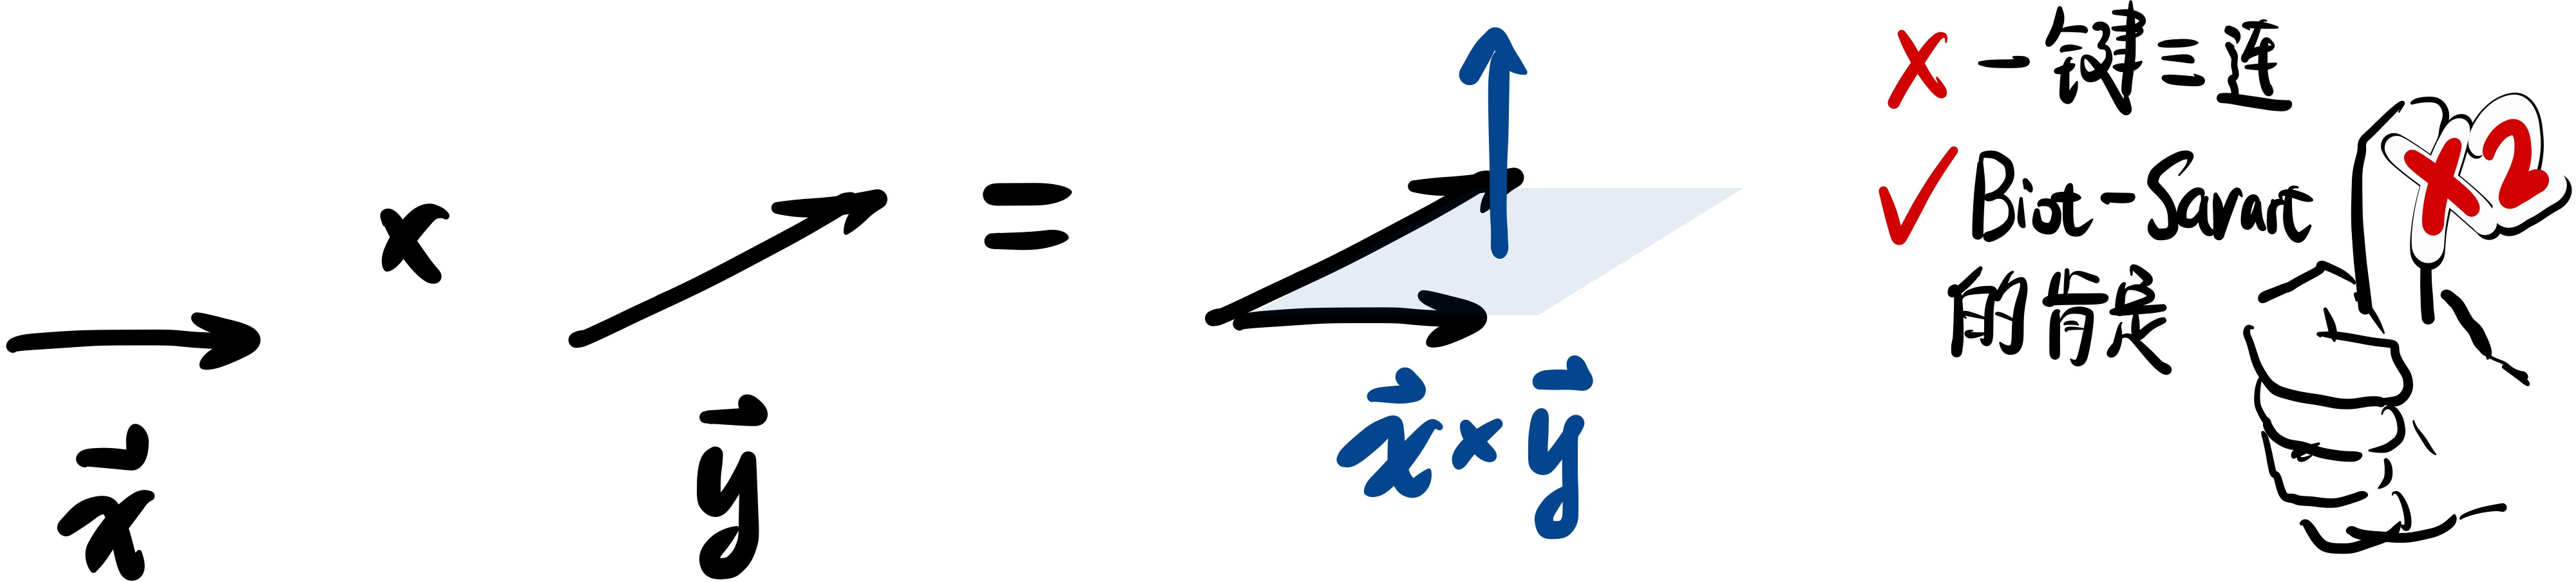
\includegraphics[width=0.9\textwidth]{img/image-20240125121748817.png}
\end{tcolorbox}

然后通量计算的就是有多少向量``通过''了一个面积, 在物理里通量常用
\(\Phi\) 表示, 考虑一个向量场 \(\boldsymbol{v}\) 和一块面积
\(\boldsymbol{A}\), 那么通量表示为这个向量场和面积向量的点乘:
\(\Phi=\boldsymbol{v}\cdot\boldsymbol{A}\). 这个结论应该是比较符合直觉 -
intuitive 的: 面积越大, 通量也越大, 向量场越``强'', 通量也越大;
向量场和面积越接近垂直 (也就是向量场的指向和面积向量的指向越一致),
有效通量越大, 对应着公式上, 因为
\(|\Phi|=|\boldsymbol{v}||\boldsymbol{A}|\cos\theta\), \(\theta\) 越接近
\(0\), \(\cos\theta\) 越接近 \(1\), 通量越大.

\section{导数算符的乘法法则}\label{029}

\begin{newquote}
注: 这一节的讨论限制在欧氏三维空间搭配直角坐标系的情况.
\end{newquote}

我们知道一元函数的导数是线性的, 不难发现, 导数算符 $\nabla$
也应该是线性的, 即有 \[
\begin{aligned}
&\nabla(af+bg)=a\nabla f+b\nabla g,\\
&\nabla\cdot(a\boldsymbol{u}+b\boldsymbol{v})=a\nabla\cdot\boldsymbol{u}+b\nabla\cdot\boldsymbol{v},\\
&\nabla\times(a\boldsymbol{u}+b\boldsymbol{v})=a\nabla\times\boldsymbol{u}+b\nabla\times \boldsymbol{v};
\end{aligned}
\] 这里 $a,b$ 是两个常数; $f,g$ 是两个标量场;
$\boldsymbol{u},\boldsymbol{v}$ 是两个向量场.
可以利用分量运算来验证上述规则.

乘法法则则相对复杂, 我们可以有四种情况:

\begin{enumerate}
\def\labelenumi{\arabic{enumi}.}

\item
  两个标量场相乘得到一个标量场;
\item
  两个向量场点乘得到一个标量场;
\item
  一个标量场乘一个向量场得到一个向量场;
\item
  两个向量场叉乘得到一个向量场.
\end{enumerate}

若结果是标量场, 我们可以求它的梯度, 而对于向量场, 我们可以求旋度和散度;
省略掉一些计算上的细节 (还是, 可以考虑分量来验证), 有结论如下: \[
\boxed{\begin{aligned}
&\nabla(fg)=f\nabla g+g\nabla f,\\
&\nabla(\boldsymbol{u}\cdot\boldsymbol{v})=\boldsymbol{u}\times(\nabla\times\boldsymbol{v})+\boldsymbol{v}\times(\nabla\times\boldsymbol{u})+(\boldsymbol{u}\cdot \nabla)\boldsymbol{v}+(\boldsymbol{v}\cdot \nabla)\boldsymbol{u},\\
&\nabla\cdot(f\boldsymbol{v})=f(\nabla\cdot\boldsymbol{v})+\boldsymbol{v}\cdot(\nabla f),\\
&\nabla\cdot(\boldsymbol{u}\times\boldsymbol{v})=\boldsymbol{u}\cdot(\nabla\times\boldsymbol{v})-\boldsymbol{v}\cdot(\nabla\times\boldsymbol{u}),\\
&\nabla\times(f\boldsymbol{v})=f(\nabla\times\boldsymbol{v})-\boldsymbol{v}\times(\nabla f);\\
&\nabla\times(\boldsymbol{u}\times\boldsymbol{v})=(\boldsymbol{v}\cdot\nabla)\boldsymbol{u}-(\boldsymbol{u}\cdot\nabla)\boldsymbol{v}+\boldsymbol{u}(
\nabla\cdot\boldsymbol{v})-\boldsymbol{v}(
\nabla\cdot\boldsymbol{u}).
\end{aligned}}
\] 上面, 例如第二个和第五个式子, 都出现了导数算符 $\nabla$
没有\textbf{直接}作用在函数 (either 标量场 or 向量场) 上的情况,
初看可能会较为费解, 但是把导数算符写成
$\nabla=\partial_x\hat{\imath}+\partial_y\hat{\jmath}+\partial_z\hat{k}$
这样一个类似``向量''的东西再运算就明确很多了.

\subsection{二次导}

\textbf{梯度的散度} \[
\begin{aligned}
\boxed{\nabla\cdot(\nabla f)}&=(\partial_x\hat{\imath}+\partial_y\hat{\jmath}+\partial_z\hat{k})\cdot\left(\frac{\partial f}{\partial x}\hat{\imath}+\frac{\partial f}{\partial y}\hat{\jmath}+\frac{\partial f}{\partial z}\hat{k}\right)\\
&\boxed{=\frac{\partial^2 f}{\partial x^2}+\frac{\partial^2 f}{\partial y^2}+\frac{\partial^2 f}{\partial z^2}}.
\end{aligned}
\] 梯度的散度常常简写为 $\nabla^2$ 或者 $\Delta$,
称作拉\textbf{普拉斯算子} (Laplacian). 拉普拉斯算子也可以作用在向量场上,
\[
\boxed{(\nabla\cdot\nabla)\cdot\boldsymbol{v}:=\nabla^2\boldsymbol{v}=(\nabla^2v_x)\hat{\imath}+(\nabla^2v_y)\hat{\jmath}+(\nabla^2v_z)\hat{k}}.
\]

\textbf{梯度的旋度} \[
\boxed{\nabla\times(\nabla f)\equiv0}.
\] 梯度的散度恒等于零. 有一个不正确的``理解'' (但是可以当作记忆法) 是,
如果把导数算符看作向量, 那么梯度的旋度便是导数算符的叉乘,
一个向量和自己的叉乘总是为零. 事实上, 若要得到这个结论,
需要用到导数算符\textbf{无挠} (torsion-free) 的性质,
这个性质并不是导数算符自带的,
而是欧氏三维空间搭配直角坐标系带来的一个好的性质, to be specific,
我们有类似 \[
\frac{\partial}{\partial x}\left(\frac{\partial f}{\partial y}\right)=\frac{\partial}{\partial y}\left(\frac{\partial f}{\partial x}\right),
\] 然后利用分量运算便很好验证.

\textbf{散度的梯度} 很少在理工科的语境中被使用到,
也没有太值得关注的规律, 甚至没有专有的称谓, 这里就不作展开.
唯一要注意的是它不等于拉普拉斯算子作用于向量场.

\textbf{旋度的散度} \[
\boxed{\nabla\cdot(\nabla\times\boldsymbol{v})=0}.
\] 旋度的散度恒为零. Again, 利用分量加以导数算符的无挠性易证. 记忆时,
可类比向量的
$\boldsymbol{a}\cdot(\boldsymbol{b}\times\boldsymbol{c})=(\boldsymbol{a}\times\boldsymbol{b})\cdot\boldsymbol{c}$
(可以自行验证), 于是又会有 $\nabla\times\nabla$ 项出现 which
可以视作一个向量和其自身的叉乘于是总是为零.

\textbf{旋度的旋度} \[
\boxed{\nabla\times(\nabla\times\boldsymbol{v})=\nabla(\nabla\cdot\boldsymbol{v})-\nabla^2\boldsymbol{v}}.
\] 记忆时, 可以类比向量三重积的 bac-cab rule, 即
$\boldsymbol{a}\times\boldsymbol{b}\times\boldsymbol{c}=\boldsymbol{b}(\boldsymbol{a}\cdot\boldsymbol{c})-\boldsymbol{c}(\boldsymbol{a}\cdot\boldsymbol{b})$
(可以自行验证). 当然, 严格一点应该依旧利用分量运算.

\section{积分 - revisited}\label{030}

\subsection{多重积分}

多重积分不是这一节的重点, 因此仅以较少的篇幅带过. 通常的 (一重) 定积分,
几何含义可以是计算函数图像下的面积, 类似的,
二重积分可以是计算一个曲面下方的体积 (如下图所示).

\begin{tcolorbox}[size=fbox, breakable, enhanced jigsaw]
    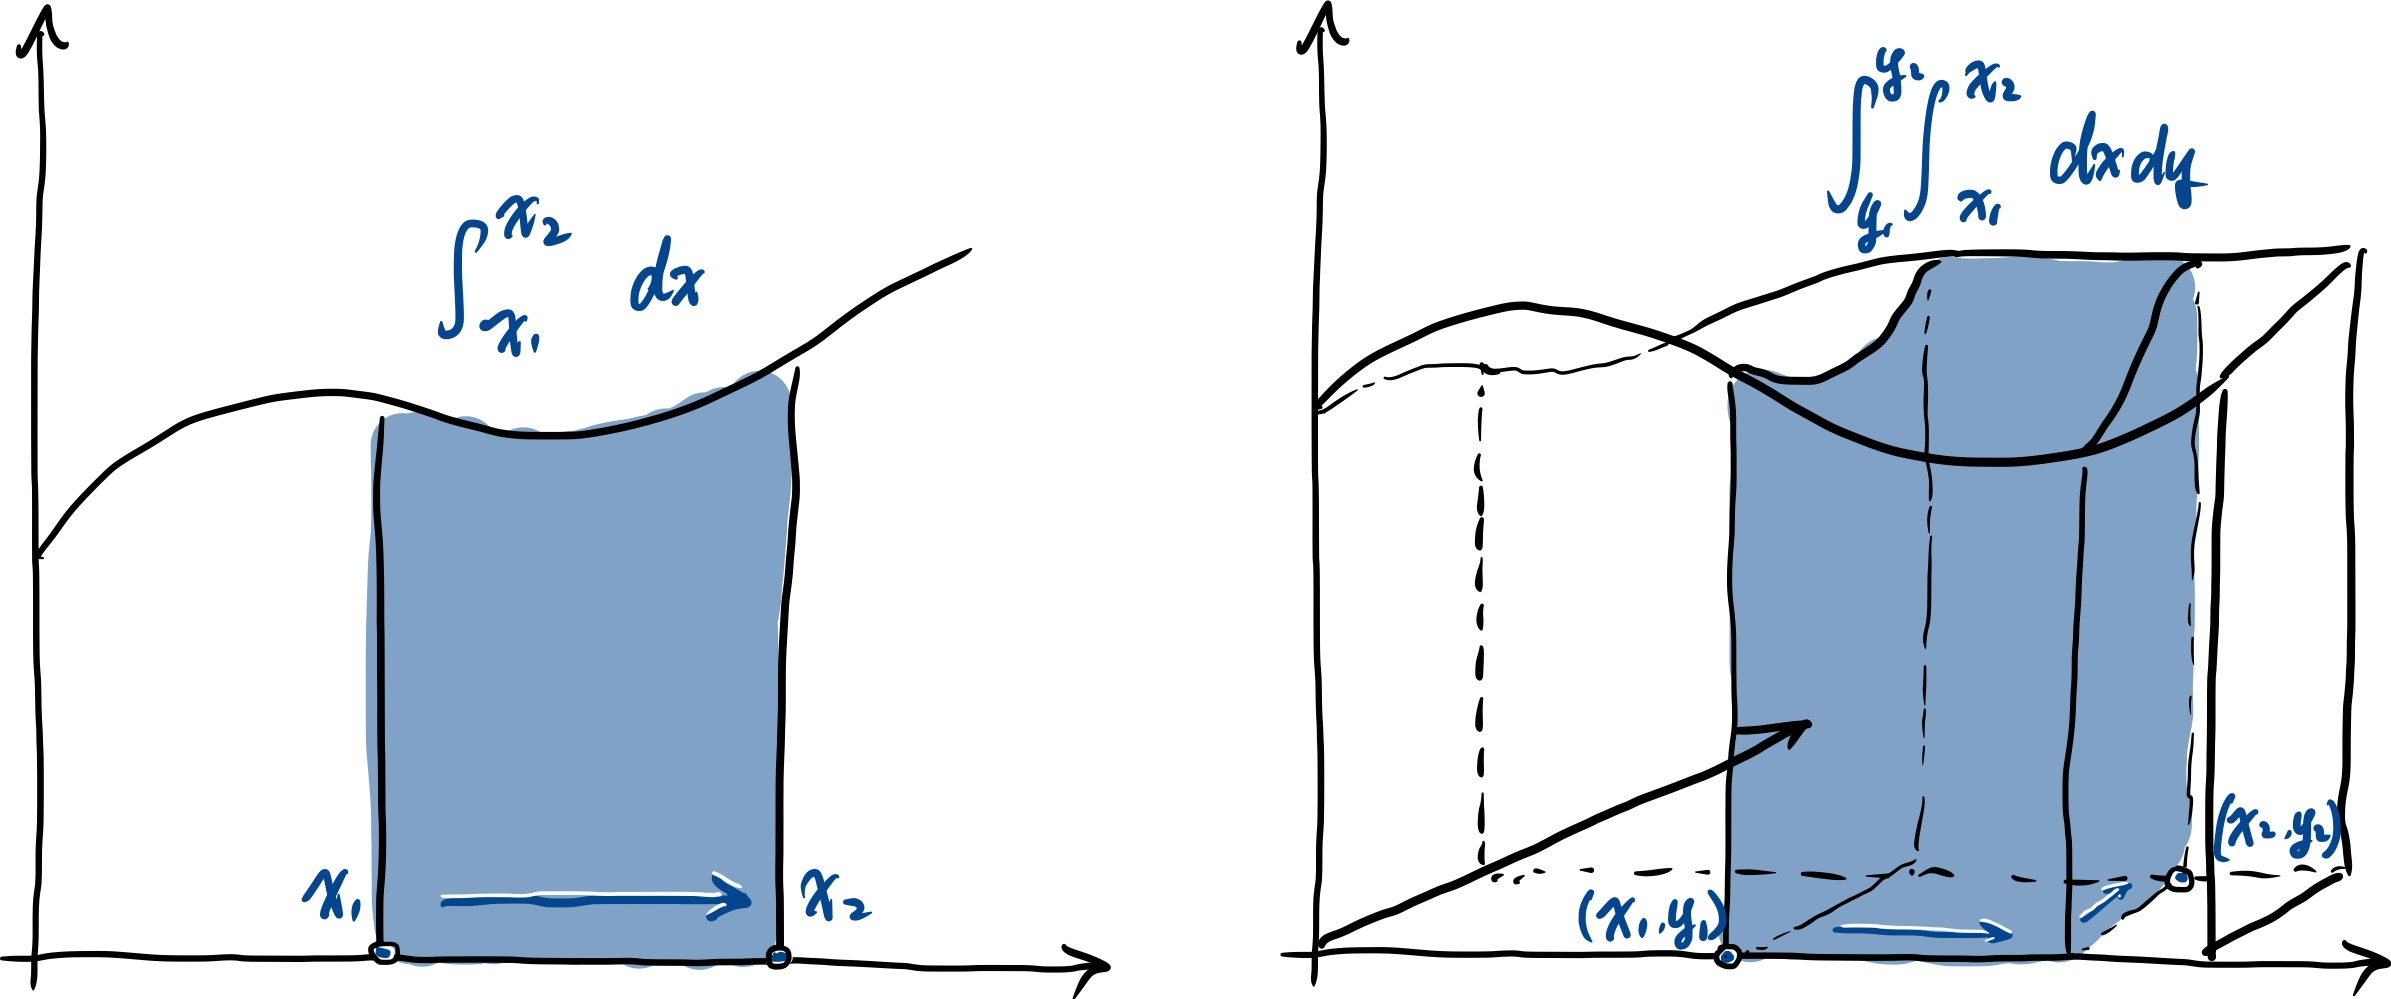
\includegraphics[width=0.9\textwidth]{./img/image-20240530065714806.png}
\end{tcolorbox}

对于三重积分, 我们可以参考前面的,
把它理解成一个三维``超曲面''在四维的空间中下方的四维``超体积'',
或者换一个思路, 我们可以考虑一个密度不均匀的三维物体,
其密度关于位置的函数给定, 已知其形状 (建立坐标系,
其形状可以用于决定积分的上下限) 的情况下, 它的质量就是一个三重积分
(回顾【\ref{019}\nameref{019}】文末).

\subsection{线积分}

英语中, 线积分 line integral 也常叫做 path integral, 可以直译作路径积分,
虽然比较直观, 但是可能和量子场论中的路径积分混淆,
所以下文还是统一做线积分. 顾名思义, 在不止一维的情况下,
对一个多元函数的积分从一个点到另一个点, 可以不止一条曲线 (路径),
所以线积分都需要 specify 积分的曲线. 线积分可能有以下几种 \[
\begin{aligned}
&\text{(i)}\ \ \int f\ \mathrm{d}\boldsymbol{r},\\
&\text{(ii)}\ \int\boldsymbol{v}\cdot\mathrm{d}\boldsymbol{r},\\
&\text{(iii)}\int\boldsymbol{v}\times\mathrm{d}\boldsymbol{r},
\end{aligned}
\] 分别是: (i) 标量场和一个``向量微元''的数乘的积分, (ii)
向量场和``向量微元''点乘的积分, (iii) 向量场和``向量微元''叉乘的积分
(三种情况如下图所示). 这里将 $\mathrm{d}\boldsymbol{r}$
称作``向量微元''并不是一个准确的描述, 通常来讲,
上述的积分都是沿着一条曲线, 所以 $\mathrm{d}\boldsymbol{r}$
作为这条曲线的一段无穷小量, 应该是切于这条曲线的一个向量 (切向量 -
tangent vector, 微分几何警告!).

\begin{tcolorbox}[size=fbox, breakable, enhanced jigsaw]
    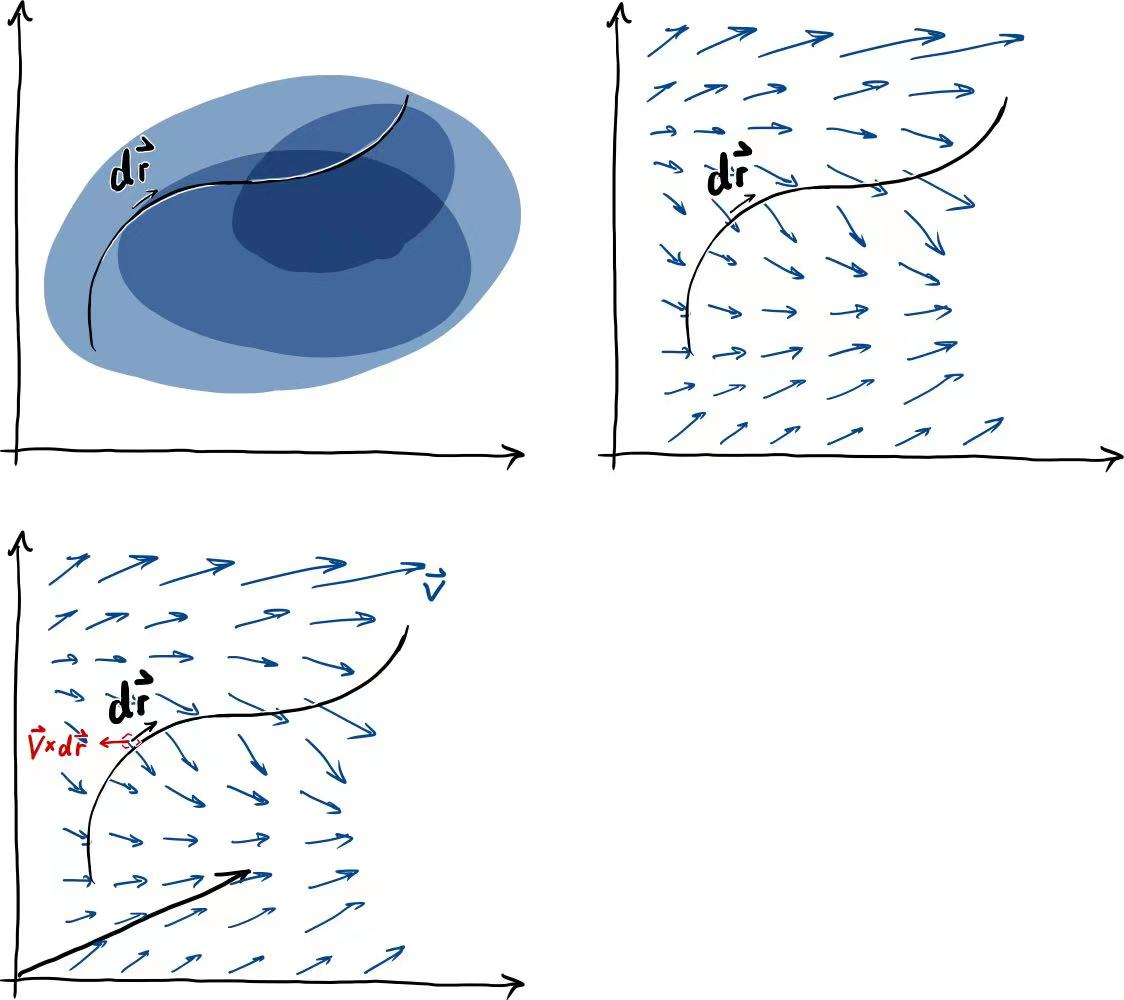
\includegraphics[width=0.9\textwidth]{./img/image-20240530065850401.png}
\end{tcolorbox}

\textbf{(i)}

考虑三维欧氏坐标系, 第一个积分可以展开作 \[
\int f\ \mathrm{d}\boldsymbol{r}=\int f(x,y,z)\mathrm{d}x\ \hat{\imath}+\int f(x,y,z)\mathrm{d}y\ \hat{\jmath}+\int f(x,y,z)\mathrm{d}z\ \hat{k},
\] 注意展开后的每一个积分, 以第一个关于 $x$ 的积分为例,
因为积分曲线是确定的, 所以 $\{y,z\}$ 不能被视作常数,
因为积分曲线已经给定, 比如以一个参数方程的形式: \[
\begin{cases}
x=x(t)\\
y=y(t)\\
z=z(t)
\end{cases},
\] 上式可以被改写为 $\{y(x),z(x)\}$, 于是在这条曲线上 $f$
可以被表述为仅关于 $x$ 的形式, 便可以对 $x$ 进行积分, 后两项也类似.
最后的结果应该是一个向量, 每一项积分的结果对应一个方向上的分量.

\begin{newquote}
考虑一条可以忽略横截面积的、密度不均匀的绳,
若其单位长度的质量以一标量场给出, 那么上述积分可以描述其质量.
\end{newquote}

\textbf{(ii)}

第二个积分是比较\textbf{常见}的, 和前面一样展开有 \[
\int\boldsymbol{v}\cdot\mathrm{d}\boldsymbol{r}=\int v_x(x,y,z)\mathrm{d}x+\int v_y(x,y,z)\mathrm{d}y+\int v_z(x,y,z)\mathrm{d}z,
\] 因为欧式坐标系中单位向量的正交归一性 (类似
$\hat{\imath}\cdot\hat{\imath}=1, \hat{\imath}\cdot\hat{k}=0$,
复习【\ref{025}\nameref{025}】), 只有上面三项是通常而言非零的, 其中 $\{v_x,v_y,v_z\}$
表示 $\boldsymbol{v}$ 的分量. 最后的结果应该是一个标量.

物理上常有做功的计算, 比如将一质点在一力场 $\boldsymbol{F}(x,y,z)$ 中,
沿一轨迹 $C(x,y,z)$ 移动, 做功便是 \[
W=\int_C\boldsymbol{F}\cdot\mathrm{d}\boldsymbol{r},
\] 其中积分符号下的 $C$ 强调积分曲线是 $C(x,y,z)$,
因为通常而言做功的大小是路径相关 (path dependent) 的,
也就是说即便是积分两端点一致, 不同的积分曲线得到的结果也会不一样.

\textbf{(iii)}

第三个积分可以展开作:

\[
\begin{aligned}
&\int\boldsymbol{v}\times\mathrm{d}\boldsymbol{r}\\
=&\int\begin{vmatrix}\hat{\imath}&\hat{\jmath}&\hat{k}\\v_x&v_y&v_z\\\mathrm{d}x&\mathrm{d}y&\mathrm{d}z\end{vmatrix}\\
=&\left(\int v_y\mathrm{d}z-\int v_z\mathrm{d}y\right)\hat{\imath}\\
&+\left(\int v_z\mathrm{d}x-\int v_x\mathrm{d}z\right)\hat{\jmath}\\
&+\left(\int v_x\mathrm{d}y-\int v_y\mathrm{d}x\right)\hat{k},
\end{aligned}
\]

叉乘不那么直观, 这样的线积分现实中也出现的较少,
但还是有一些用得到的例子.

\begin{newquote}
说到叉乘就想到右手定则 (复习【\ref{026}\nameref{026}】),
说到右手定则就想到了毕奥-萨伐尔定律 (Biot-Savart Law), which states that
\[
\boldsymbol{B}=\frac{\mu_0I}{4\pi}\int_C\frac{\mathrm{d}\boldsymbol{l}\times \boldsymbol{r}}{r^3},
\] 上式描述了通电导线产生的磁场 $\boldsymbol{B}$, $\mu_0$ 是一个常数
(真空磁导率), $I$ 是电流的大小, $\mathrm{d}\boldsymbol{l}$
是电流所在的线元, $\boldsymbol{r}$ 是线元指向待求磁场强度所在的点
(空间上我们关注的点, 在这个点上磁场强度是 $\boldsymbol{B}$), $r$ 是
$\boldsymbol{r}$ 的大小 (也就是线元到关注点的距离).

注: 其实上式中, 磁场和距离平方成反比 (i.e.~$B\propto1/r^2$), 磁场
$\boldsymbol{B}$ 的方向同时垂直于 $\boldsymbol{r}$ 和
$\mathrm{d}\boldsymbol{l}$, 所以叉乘只是希望得到磁场的方向, 但是
$\boldsymbol{r}$ 会额外 introduce 一个 $r=|\boldsymbol{r}|$ ,
所以为了消掉这个额外的 $r$, 分母便成了 $r^3$.
这也是库仑力或引力的向量公式里出现 $\boldsymbol{r}/r^3$ 的原因.
在一些记号中, 规定单位向量 $\hat{r}:=\boldsymbol{r}/r$
也可以使得公式看起来更自然, 当然也有教材使用 $\hat{e}_r$.
\end{newquote}

\subsection{面积分}

面积分也可以有几种情况: \[
\begin{aligned}
&\text{(i)}\ \ \int f\ \mathrm{d}\boldsymbol{a},\\
&\text{(ii)}\ \int\boldsymbol{v}\cdot\mathrm{d}\boldsymbol{a},\\
&\text{(iii)}\int\boldsymbol{v}\times\mathrm{d}\boldsymbol{a},
\end{aligned}
\] 稍难理解一些的是, 为什么面积会是一个向量; 事实上, 记
$a=|\boldsymbol{a}|$, 那么有
$\mathrm{d}\boldsymbol{a}=\hat{n}\mathrm{d}a$, 其中 $\hat{n}$
是面积元 $\mathrm{d}a$ 处的法向量 (normal vector). 对于一个闭曲面
(closed surface), 一般将向``外''记作法向量的正方向, 对于不封闭的单连通
(simply connected, 简单来说就是没有``洞'') 曲面 $S$,
若是给定曲面的边界 $\partial S$ (boundary) 的指向,
便可以用右手定则来决定法向量的方向.

\begin{newquote}
超纲\&剧透: 至于为什么曲面边界可以用偏导来表示, 需要一些外积, 外微分,
和微分形式的知识 (目前暂时只有在【\ref{026}\nameref{026}】的选读提及了一下外积), but in
short, generalized 的斯托克斯定律 (Stokes' theorem) 告诉我们 \[
\int_{\partial S}\omega=\int_S\mathrm{d}\omega,
\] 这里 $\omega$ 是待积分的微分形式.
狭义一点的版本的斯托克定律会在稍后呈现.
\end{newquote}

第 (ii) 个积分比较常用, 通常用来计算流量或者通量,
例如计算一个置于非匀强磁场中的环形电路围成的面积里的磁通量,
点乘的性质很好的解决了当磁感线与面积元不垂直的情况.

\subsection{体积分}

体积分大多数时候将体积元视作标量 $\mathrm{d}V$, 于是情况无非为: \[
\begin{aligned}
&\text{(i)}\ \ \int f\ \mathrm{d}V,\\
&\text{(ii)}\ \int\boldsymbol{v}\ \mathrm{d}V,
\end{aligned}
\] 通常第一个积分会比较常用, 例如已知一个物体的密度关于位置的函数,
待求这个物体的质量.

\begin{newquote}
实际上, 从外积的角度出发, 考虑三维欧氏空间中的一个平行于 $x-y$
平面的面元 $\mathrm{d}\boldsymbol{a}$ 可以写作
$(\mathrm{d}x\wedge\mathrm{d}y)$; 那么体元是不是就是
$(\mathrm{d}x\wedge\mathrm{d}y\wedge\mathrm{d}z)$ 了呢? 是也非也,
如果我们视体元为标量的化, 应该有
$\mathrm{d}V=|\mathrm{d}x\wedge\mathrm{d}y\wedge\mathrm{d}z|$,
但其实定义一个``向量''版本的体元也并非不可,
其几何含义可以仿照这二维面元, 解读为:
一个三维形状可以视作一个四维空间中的一个超曲面 (hypersurface),
于是向量体元 $(\mathrm{d}x\wedge\mathrm{d}y\wedge\mathrm{d}z)$
实际上是 $\mathbb{R}^4$ 中的一个``超曲面元''.

这样既然有了向量版本的体元, 便可以有它与向量场的点乘叉乘了 (我们日常的
$\mathbb{R}^3$ 大概是鲜有情况需要用到这一点,
不过很多利用到高维向量的学科, 例如机器学习中的支持向量机等,
类似的无用的知识点大概也许可能有点作用).
\end{newquote}

\section{微积分基本定理 - revisited - 上}\label{031}

回顾【\ref{019}\nameref{019}】, 微积分基本定理也叫\textbf{牛顿-莱布尼兹公式}
(Newton-Leibniz formula), which states that \[
\int_a^bf(x)\mathrm{d}x=F(b)-F(a),
\] 其中 $F(x)$ 是 $f(x)$ 的反导数, 即有 $F'(x)=f(x)$.
在向量微积分中, 也有类似的一些关系.

\subsection{梯度定理}

梯度定理 (gradient theorem) 可以看作是微积分基本定理的高维推广,
according to which,
\begin{equation*}
    \boxed{\int_{\boldsymbol{a}}^{\boldsymbol{b}}(\nabla f)\cdot\mathrm{d}\boldsymbol{r}=f(\boldsymbol{b})-f(\boldsymbol{a})},
\end{equation*}

区别在于, 现在 $f$ 是一个标量场而非一元函数了, 积分上下限也变作了向量.
究其本质, 在【\ref{028}\nameref{028}】引出梯度时有 \[
\mathrm{d}f=(\nabla f)\cdot\mathrm{d}\boldsymbol{r},
\] 在三维欧氏空间中展开就是 \[
\begin{aligned}
\mathrm{d}f=&\left(\frac{\partial f}{\partial x}\hat{\imath}\right)\cdot\left(\mathrm{d}x\hat{\imath}\right)+\left(\frac{\partial f}{\partial y}\hat{\jmath}\right)\cdot\left(\mathrm{d}y\hat{\jmath}\right)+\left(\frac{\partial f}{\partial z}\hat{k}\right)\cdot\big(\mathrm{d}z\hat{k}\big)\\
=&\frac{\partial f}{\partial x}\mathrm{d}x+\frac{\partial f}{\partial y}\mathrm{d}y+\frac{\partial f}{\partial z}\mathrm{d}z,
\end{aligned}
\] 于是很自然地有 \[
\begin{aligned}
&\int(\nabla f(x,y,z))\cdot\mathrm{d}\boldsymbol{r}\\
=&\int\mathrm{d}f\\
=&\int\frac{\partial f}{\partial x}\mathrm{d}x+\frac{\partial f}{\partial y}\mathrm{d}y+\frac{\partial f}{\partial z}\mathrm{d}z\\
=&f(x,y,z),
\end{aligned}
\] 就有了 \[
\begin{aligned}
\int_{(x_1,y_1,z_1)}^{(x_2,y_2,z_3)}(\nabla f(x,y,z))\cdot\mathrm{d}\boldsymbol{r}=&f(x,y,z)\left|_{(x_1,y_1,z_1)}^{(x_2,y_2,z_3)}\right.\\
=&f(x_2,y_2,z_2)-f(x_1,y_1,z_1).
\end{aligned}
\] 不难发现, 对于梯度的线积分是路径无关的 (path-independent),
因为最终的结果只和起止的端点相关, 等价地,
也可以说如果梯度的积分曲线是闭合的, 则结果为零,
i.e.~$\oint(\nabla f)\cdot\mathrm{d}\boldsymbol{r}=0$. 进一步地,
我们可以说, 若一个向量场可以表述为一个标量场的梯度,
那么它的线积分便是路径无关的.

\subsection{格林定理}

在把类似得结论推广到散度和旋度上之前, 稍稍来一点小插曲. 考虑二维的情况,
有一向量场 $\boldsymbol{v}=v_x\hat{\imath}+v_y\hat{\jmath}$,
然后再考虑 $\oint_C\boldsymbol{v}\cdot\mathrm{d}\boldsymbol{r}$
这样一个闭合曲线上的积分.
这个积分可以被``拆解''成许多个小的闭合路径上的积分之和 (如下图所示) ,
因为沿曲线积分是有方向的, 所以拆分成许多个小的闭合路径上的积分之和时,
那些重复计算的部分会因为积分时方向不同被抵消, 类似
$\int_a^bf\mathrm{d}x+\int_b^af\mathrm{d}x=0$.
现在关注一个小的闭合路径上的积分, 方便起见, 将路径定位一个矩形边界
(当然, 得出的结论应该时 true in general 的), 如下图右所示,
这个积分可以表示为 \[
\begin{aligned}
\int_{C_{ij}}\boldsymbol{v}\cdot\mathrm{d}\boldsymbol{r}=&\int_{(x_i,y_{j+1})
}^{(x_{i+1},y_{j+1})}\boldsymbol{v}\cdot\mathrm{d}\boldsymbol{r}+\int_{(x_{i+1},y_{j+1})
}^{(x_{i+1},y_j)}\boldsymbol{v}\cdot\mathrm{d}\boldsymbol{r}\\
&+\int_{(x_{i+1},y_j)
}^{(x_i,y_j)}\boldsymbol{v}\cdot\mathrm{d}\boldsymbol{r}+\int_{(x_i,y_j)
}^{(x_i,y_{j+1})}\boldsymbol{v}\cdot\mathrm{d}\boldsymbol{r}.
\end{aligned}
\] 

\begin{tcolorbox}[size=fbox, breakable, enhanced jigsaw]
    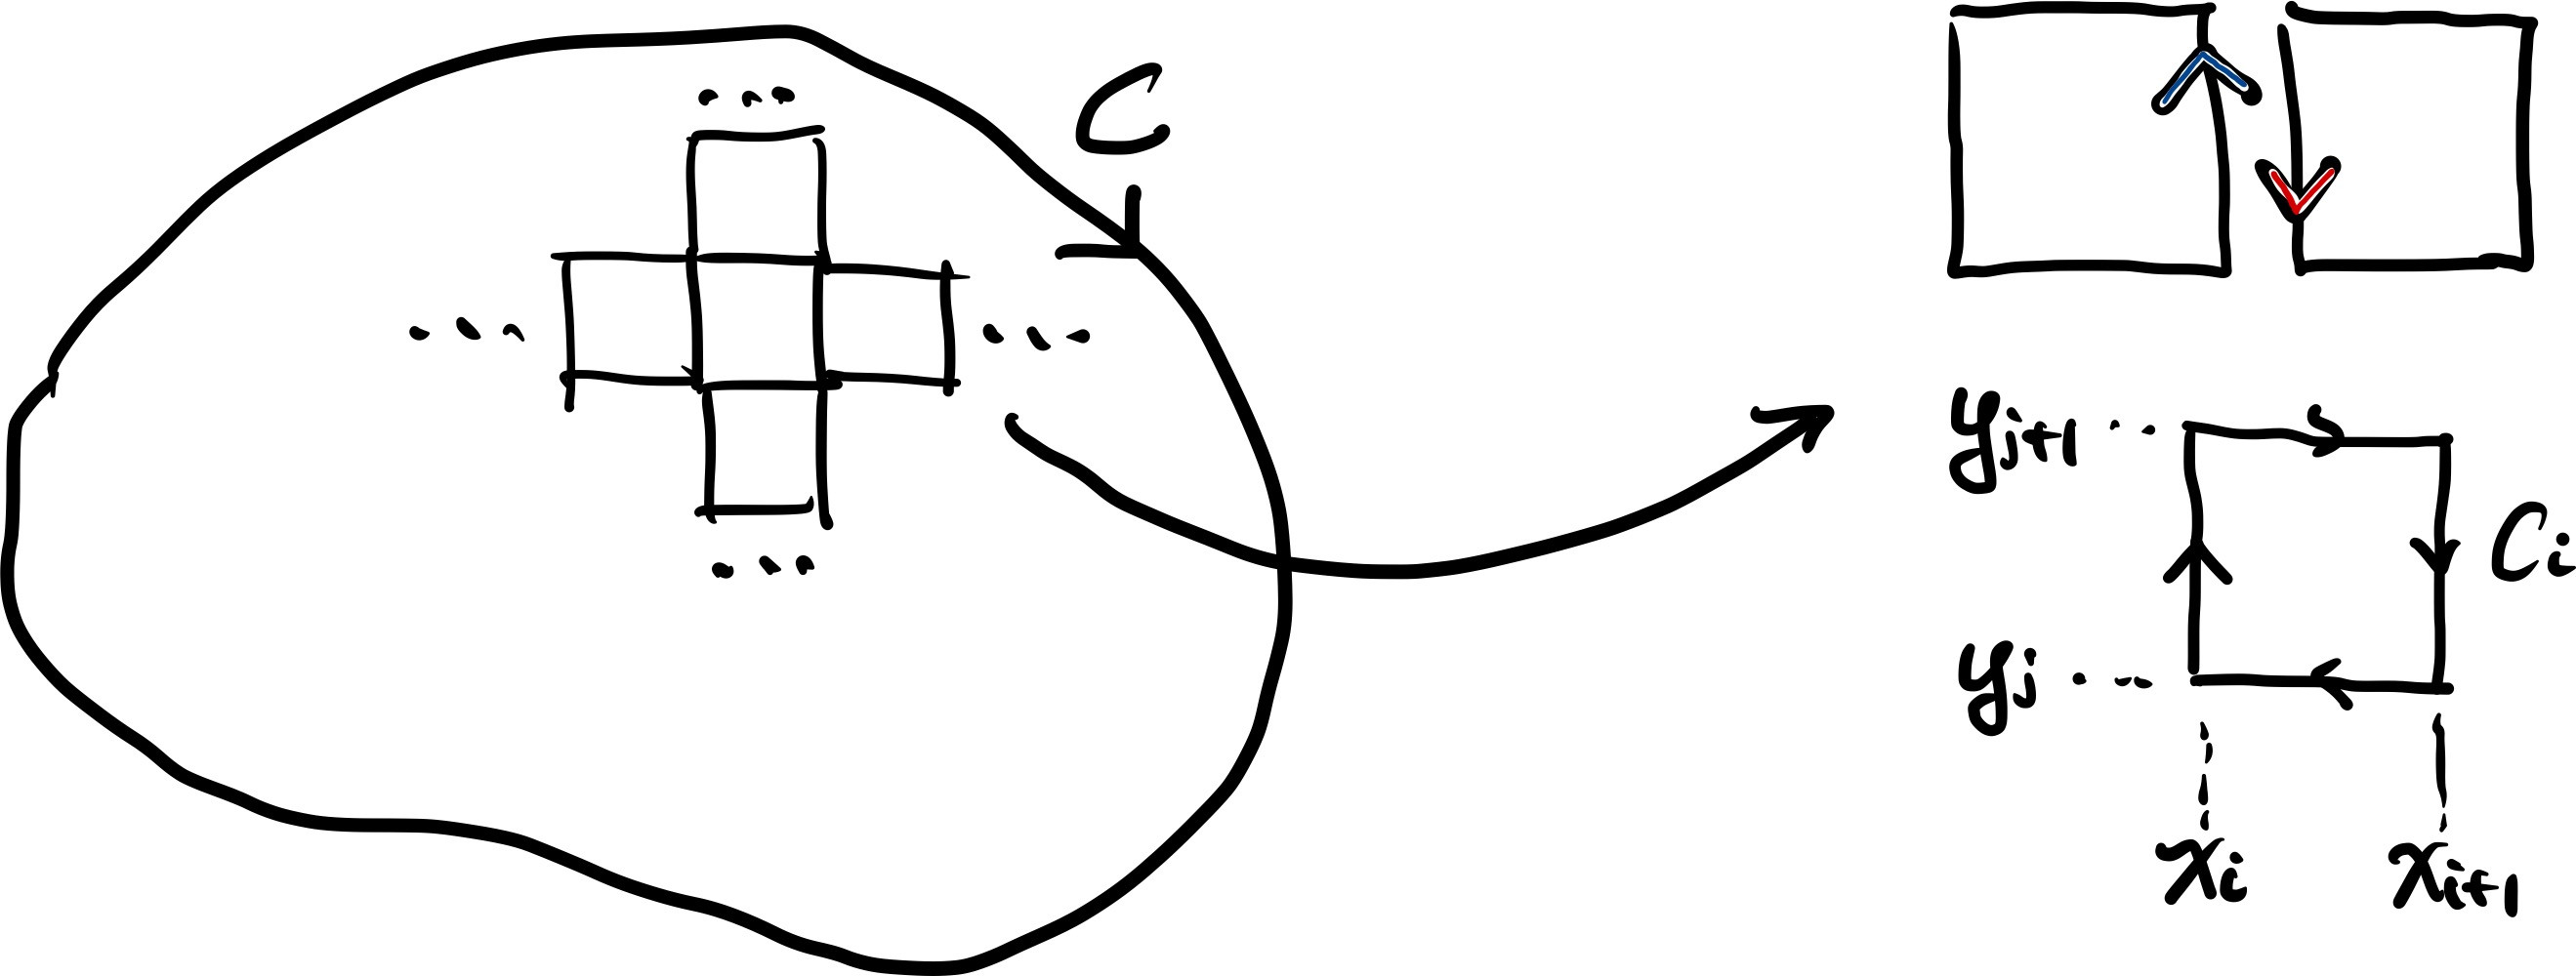
\includegraphics[width=0.9\textwidth]{./img/image-20240604044203628.png}
\end{tcolorbox}

根据 $\boldsymbol{v}$ 的定义, 以及
$\mathrm{d}\boldsymbol{r}=\mathrm{d}x\hat{\imath}+\mathrm{d}y\hat{\jmath}$,
利用点乘的性质, 不难发现事实上 \[
\begin{aligned}
\oint_{C_{ij}}\boldsymbol{v}\cdot\mathrm{d}\boldsymbol{r}=&\int_{(x_i,y_{j+1})
}^{(x_{i+1},y_{j+1})}v_x\mathrm{d}x+\int_{(x_{i+1},y_{j+1})
}^{(x_{i+1},y_j)}v_y\mathrm{d}y\\
&+\int_{(x_{i+1},y_j)
}^{(x_i,y_j)}v_x\mathrm{d}x+\int_{(x_i,y_j)
}^{(x_i,y_{j+1})}v_y\mathrm{d}y,\\
=&\int_{x_i
}^{x_{i+1}}v_x\Big|_{y=y_{j+1}}\mathrm{d}x+\int_{y_{j+1}
}^{y_j}v_y\Big|_{x=x_{i+1}}\mathrm{d}y\\
&+\int_{x_{i+1}
}^{x_i}v_x\Big|_{y=y_{j}}\mathrm{d}x+\int_{y_j
}^{y_{j+1}}v_y\Big|_{x=x_{i}}\mathrm{d}y,\\
=&\int_{x_i}^{x_{i+1}}\left(v_x\Big|_{y=y_{j+1}}-v_x\Big|_{y=y_j}\right)\mathrm{d}x\\&-\int_{y_i}^{y_{i+1}}\left(v_y\Big|_{x=x_{i+1}}-v_y\Big|_{x=x_i}\right)\mathrm{d}y.
\end{aligned}
\] 最后利用本节开头回顾的微积分基本定理, 有 \[
\begin{aligned}
v_x\Big|_{y=y_{j+1}}-v_x\Big|_{y=y_j}=\int_{y_j}^{y_{j+1}}\frac{\partial}{\partial y}v_x\mathrm{d}y,\\
v_y\Big|_{x=x_{i+1}}-v_y\Big|_{x=x_i}=\int_{x_i}^{x_{i+1}}\frac{\partial}{\partial x}v_u\mathrm{d}x.
\end{aligned}
\] 这样一来在一个小的闭合路径中便有 \[
\oint_{C_{ij}}\boldsymbol{v}\cdot\mathrm{d}\boldsymbol{r}=\int_{x_i}^{x_{i+1}}\int_{y_j}^{y_{j+1}}\left(\frac{\partial v_x}{\partial y}-\frac{\partial v_y}{\partial x}\right)\mathrm{d}y\mathrm{d}x.
\]

根据前面的论述, 整个延封闭曲线的积分可以视作这些小的闭合路径的积分之和,
即 \[
\oint_C\boldsymbol{v}\cdot\mathrm{d}\boldsymbol{r}=\sum_{i,j}\oint_{C_{ij}}\boldsymbol{v}\cdot\mathrm{d}\boldsymbol{r}.
\]
和这些小的闭合路径等价的二重积分对应的``面积''事实上是闭合路径围出的面积,
求和后对应的面积之和也就应该变为整个封闭曲线所围成的面积, 所以有 \[
\boxed{\oint_{\partial S}\boldsymbol{f}\cdot\mathrm{d}\boldsymbol{r}=\iint_S\left(\frac{\partial v_x}{\partial y}-\frac{\partial v_y}{\partial x}\right)\mathrm{d}A},
\] 即对一向量场沿着闭合曲线的积分,
等于其分量偏导之差的关于这一闭合曲线围成的平面的面积分; 这里为了
consistency, 将平面记作 $S$, 这个平面的边界记作 $\partial S$.

\begin{newquote}
待考证: 可能因为积分正方向取顺/逆时针, 上式右边和其他版本差了一个符号.
\end{newquote}

这个结论叫做\textbf{格林定理} (green theorem) 的环量形式 (circulation
form), 或者说切形式 (tangential form). 叫环量是因为,
我们接下来马上要看到, 它和旋度的定理很像, 甚至
$\left(\frac{\partial v_x}{\partial y}-\frac{\partial v_y}{\partial x}\right)$
这个形式有时被叫做 ``s-curl'' - ``scalar curl'' (所谓标量旋度,
旋度的二维类比). 叫切形式是因为 $\mathrm{d}\boldsymbol{r}$
是切于积分曲线的.

既然有切形式, 很自然就要问, 有没有法形式 (normal form) 呢? 有: \[
\boxed{\oint_{\partial S}\boldsymbol{f}\cdot\mathrm{d}\boldsymbol{n}=\iint_S\left(\frac{\partial v_x}{\partial y}+\frac{\partial v_y}{\partial x}\right)\mathrm{d}A},
\] 虽然还是沿着一条闭合曲线去积分, 但是切向量
$\mathrm{d}\boldsymbol{r}$ 换成了法向量 $\mathrm{d}\boldsymbol{n}$,
所以切形式的情况中 $v_x\mathrm{d}x$ 和 $v_y\mathrm{d}y$ 的项就变成了
$v_x\mathrm{d}y$ 和 $v_y\mathrm{d}x$.
这个结论也叫做格林定理的通量形式 (flux form),
不难猜它和接下来的散度定理很像.

\section{微积分基本定理 - revisited - 下}\label{032}

\subsection{散度定理}

散度定理又叫做\textbf{高斯定理} (Gauss's theorem), in which \[
\boxed{\oiint\boldsymbol{v}\cdot\mathrm{d}\boldsymbol{a}=\iiint\nabla\cdot\boldsymbol{v}\ \mathrm{d}V},
\] 即在一闭合区域内, 【其边界所对应的闭合曲面上的, 这个向量场的面积分】,
等于【对一个向量场的散度的体积分】.

证明思路和格林定理的味道很像,
事实上散度定理确实可以看作是二维的格林定理法形式或者通量形式
(参见【\ref{031}\nameref{031}】) 在三维的推广.

首先, 面积分 $\oiint\boldsymbol{v}\cdot\mathrm{d}\boldsymbol{a}$
可以''拆解''成许多个小的体积表面上的积分之和 (如下图所示),
因为通量积分是定向的, 所以重复计算的部分会因为方向不同而抵消.
现在关注一块小的体积表面上的积分, 方便起见,
将小的体积定为棱平行于坐标轴的一个立方体, 这样一来, 积分
$\oiint\boldsymbol{v}\cdot\mathrm{d}\boldsymbol{a}$
可以大致分成三个方向上的积分: 上-下面、左-右面、前-后面.

\begin{tcolorbox}[size=fbox, breakable, enhanced jigsaw]
    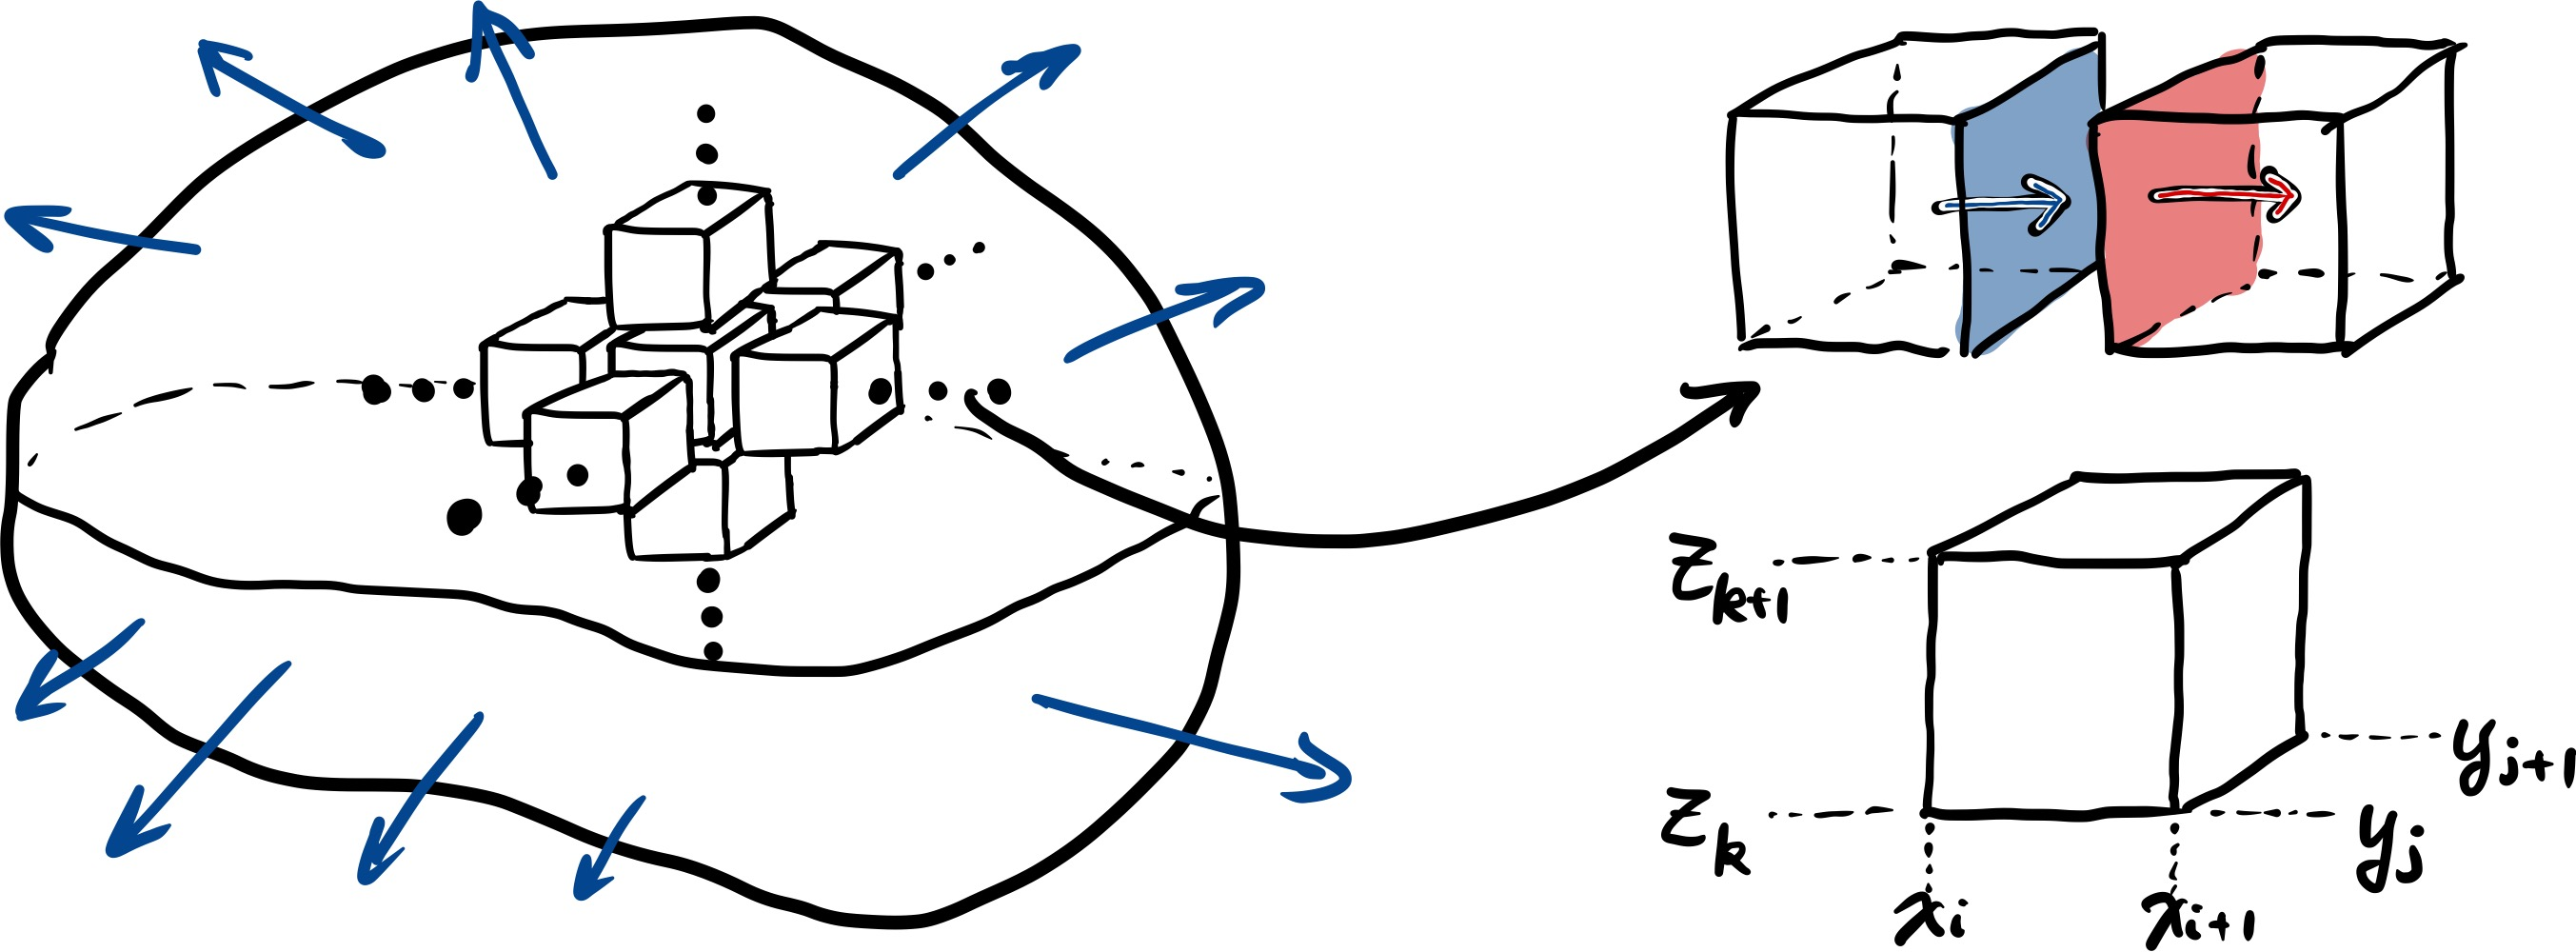
\includegraphics[width=0.9\textwidth]{./img/image-20240618231420999.png}
\end{tcolorbox}

以上-下面上的通量积分为例, 在一块小的体积上, 它应该为 \[
v_z\big|_{z=z_{k+1}}\cdot(y_{j+1}-y_{j})\cdot(x_{i+1}-x_i)-v_z\big|_{z=z_{k}}\cdot(y_{j+1}-y_{j})\cdot(x_{i+1}-x_i),
\] 这里 $v_z$ 代表向量场 $\boldsymbol{v}$ 平行于 $z$-轴的分量,
即有 \[\boldsymbol{z}=v_x\hat{\imath}+v_y\hat{\jmath}+v_z\hat{k}\].

\begin{newquote}
另外, 在 evaluate $v_z$ 时, 我们忽略代入不同的 $x$ 和 $y$ 的影响,
只考虑 $z$ 值不同导致 $v_z$ 的变化; 但实际上 $x$ 和 $y$
的取值当然会影响 $v_z(x,y,z)$, 尤其是在一个有限的平面上,
但是稍后我们就会将我们所关注的小立方的体积推至无穷小,
这样它的各个表面也会变得无穷小, $v_z$ 的取值也缩到某个固定的 $x$ 和
$y$ 上了.
\end{newquote}

然后利用微积分基本定理 (回顾【\ref{031}\nameref{031}】开头), 会有上-下面上的通量积分为 \[
\int_{z_k}^{z_{k+1}}\frac{\partial v_z}{\partial z}\mathrm{d}z\Delta x\Delta y,
\] 这里 $\Delta x=(x_{i+1}-x_i)$, $\Delta y=(y_{j+1}-y_{j})$.
当我们将小立方变为一个体积微元, 即取 $\Delta x\rightarrow \mathrm{d}x$
以及 $\Delta y\rightarrow\mathrm{d}y$, 它上-下面的通量微元变为 \[
\frac{\partial v_z}{\partial z}\mathrm{d}z\mathrm{d}x\mathrm{d}y.
\] 类似的, 左-右面和前-后面的通量微元分别应为 \[
\frac{\partial v_x}{\partial x}\mathrm{d}x\mathrm{d}y\mathrm{d}z,\frac{\partial v_y}{\partial y}\mathrm{d}x\mathrm{d}y\mathrm{d}z.
\] 整个体积微元表面上的通量之和便是 \[
\left(\frac{\partial v_x}{\partial x}+\frac{\partial v_y}{\partial y}+\frac{\partial v_z}{\partial z}\right)\mathrm{d}x\mathrm{d}y\mathrm{d}z.
\] 这样一来, 一个有限的体积表面上的通量, 例如先前考虑的小立方体, 应为 \[
\int_{z_k}^{z_{k+1}}\int_{y_j}^{y_{j+1}}\int_{x_i}^{x_{i+1}}\left(\frac{\partial v_x}{\partial x}+\frac{\partial v_y}{\partial y}+\frac{\partial v_z}{\partial z}\right)\mathrm{d}x\mathrm{d}y\mathrm{d}z.
\] 继而小立方所构成的整个体积表面上的通量就是 \[
\begin{aligned}
&\oiint\boldsymbol{v}\cdot\mathrm{d}\boldsymbol{a}\\
=&\sum_{i,j,k}\int_{z_k}^{z_{k+1}}\int_{y_j}^{y_{j+1}}\int_{x_i}^{x_{i+1}}\left(\frac{\partial v_x}{\partial x}+\frac{\partial v_y}{\partial y}+\frac{\partial v_z}{\partial z}\right)\mathrm{d}x\mathrm{d}y\mathrm{d}z\\
=&\iiint\left(\frac{\partial v_x}{\partial x}+\frac{\partial v_y}{\partial y}+\frac{\partial v_z}{\partial z}\right)\mathrm{d}x\mathrm{d}y\mathrm{d}z.
\end{aligned}
\] 不难发现, 最后一行括号内的项实际上就是 $\boldsymbol{v}$ 的散度
$\nabla\cdot\boldsymbol{v}$, 于是证毕.

\subsection{旋度定理}

旋度定理又叫做\textbf{斯托克斯定理} (Stokes' theorem), \[
\boxed{\oint\boldsymbol{v}\cdot\mathrm{d}\boldsymbol{r}=\iint\nabla\times\boldsymbol{v}\cdot\mathrm{d}\boldsymbol{a}},
\] 即在一个曲面上, 【其边界, 也就是一个闭合曲线上的一个向量场的线积分】,
等于【这个向量场的旋度在这个曲面上的面积分】.

证明思路和格林定理的味道还是很像,
而且事实上旋度定理又是二维的格林定理切形式或者环量形式 (参见【\ref{031}\nameref{031}】)
在三维的推广.

假设有一简单曲面, 选取一个合适的坐标系, 使得其可以被表示为 $z(x,y)$
的形式,

\begin{tcolorbox}[size=fbox, breakable, enhanced jigsaw]
    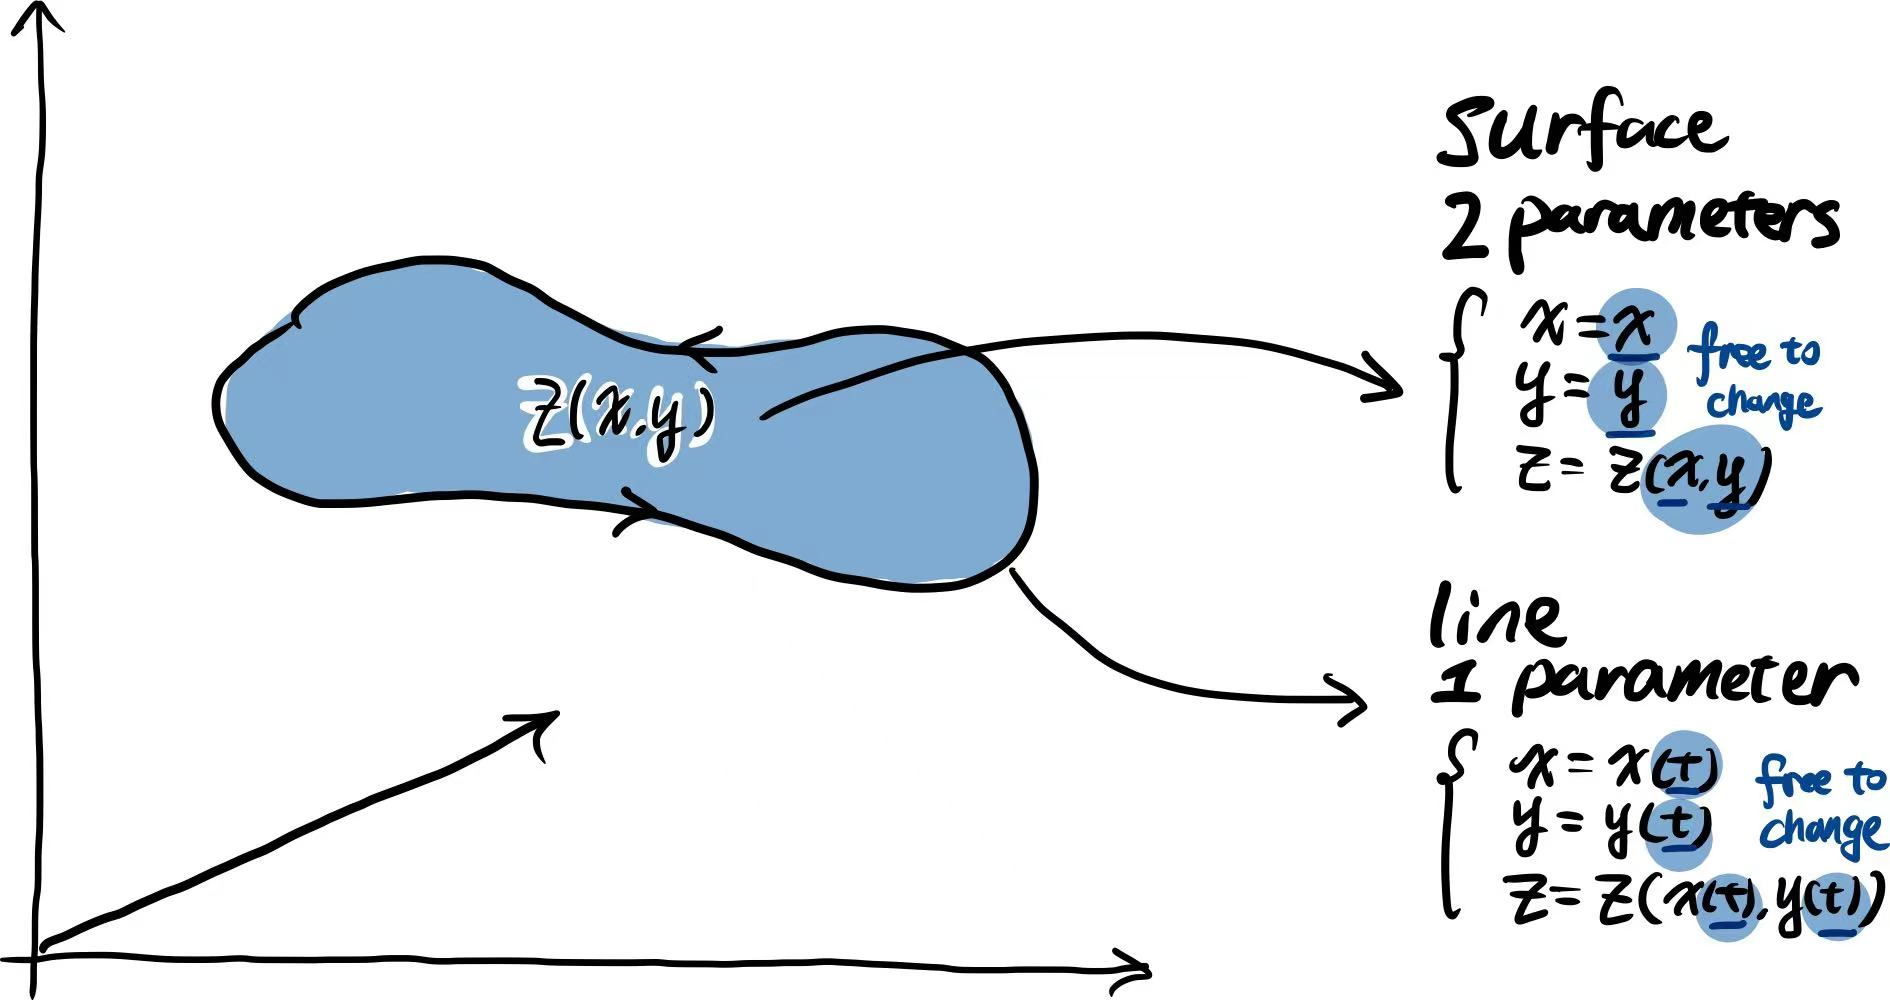
\includegraphics[width=0.9\textwidth]{./img/image-20240621050652898.png}
\end{tcolorbox}

\begin{newquote}
即给定某个 $(x,y)$ 位置, 这个平面的高度 $z$ 可以被确定;
当然旋转坐标轴, 用类似 $x(y,z)$ 的形式表示也完全没问题;
甚至可以利用参数化 (parametrization), 因为一个平面是二维的,
所以两个自由度就可以确定一个平面, 选定参数$\{s,t\}$,
平面还可以表示为形如 \[
\begin{cases}
x(s,t)\\
y(s,t)\\
z(s,t)
\end{cases}
\] 的参数化平面.
\end{newquote}

因为这个平面是二维的, 所以这个平面上某点的切向量是无限多的,
但是我们可以选定两个基向量 (复习【\ref{025}\nameref{025}】),
然后其他的向量便可以由这两个基向量张 (span) 成. 在【\ref{030}\nameref{030}】的线积分中,
我们提到过 $\mathrm{d}\boldsymbol{r}$ 的几何含义应该是曲线的切向量,
那么推广到曲面上, 切向量的基向量比较''自然''的选择便是
$1\hat{\imath}+0\hat{\jmath}+(\partial z/\partial x)\hat{k}$ 和
$0\hat{\imath}+1\hat{\jmath}+(\partial z/\partial y)\hat{k}$.

\begin{newquote}
这看起来一点都不''自然''. 这里''简单''且不严格地扩充一下,
来一个''天地联通'':

地: 比较接地气的铺垫, 我们在看多元函数的变化率时 (复习【\ref{023}\nameref{023}】),
因为函数时关于多个变量的, 在某个取值下, 函数并没有''唯一''的变化率; 比如
$f(x,y)$, 在某个特定的点 $(x,y)$ 上, $f$ 的变化率并不唯一, 最沿着
$x$ 的方向上它有一个变化率, 沿着 $y$ 的方向上有另一个变化率, 沿着
$y=x$ 的方向上还有一个不同的变化率; 为此, 只有声明好一个特定的方向,
才有一个唯一的变化率, 这样的变化率用\textbf{方向导数} (directional
derivative) 来给出, 方向的声明通常经由一个 (单位) 向量
$\boldsymbol{v}$ 给出,
然后一个多元函数的方向导数便可以表示为这个函数的梯度点乘上这个向量,
i.e.~$\nabla f\cdot\boldsymbol{v}$, (回顾【\ref{028}\nameref{028}】提及的梯度下降法).
若将函数 $f$ 看作一个平面, 那么梯度 $\nabla f$
可以视作一个特殊的切于这个平面的向量, 它所在的方向变化率最大, in
general, 偏导这个操作似乎是给出了平行于某个坐标轴的切向量.

天: (剧透警告) 既然偏导这个操作可以给出切向量, 在\textbf{微分几何}
(differential geometry) 中, 给一个流形上某点的领域选定坐标系,
该点处的所有切向量可以被 $\{\partial/\partial_{x_n}\}$ 线性表出
(即任意切向量 $\boldsymbol{T}$ 可以展开成
$\boldsymbol{T}=\sum_na_n\partial/\partial_{x_n}$, $a_n$ 是分量,
$\partial/\partial_{x_n}$ 充当基底, 回顾【\ref{024}\nameref{024}】文末的讨论),
(当然这个表示其实省略了偏导要作用在一个对象上,
类似这种省略作用对象的标记在很多场合常有出现).

因为现在我们的平面用参数化地视角看是 \[
\begin{cases}
x=x\\
y=y\\
z=z(x,y)
\end{cases}
\] 其中 $\{x,y\}$ 可以看作参数, 于是 $\partial/\partial_{x}$ 和
\[\partial/\partial_{y}\] 对应的两个基向量便是 \[
\begin{aligned}
\boldsymbol{T}_1=\frac{\partial}{\partial x}\left(x\hat{\imath}+y\hat{\jmath}+z(x,y)\hat{k}\right)&=1\hat{\imath}+0\hat{\jmath}+\frac{\partial z}{\partial x}\hat{k},\\
\boldsymbol{T}_2=\frac{\partial}{\partial y}\left(x\hat{\imath}+y\hat{\jmath}+z(x,y)\hat{k}\right)&=0\hat{\imath}+1\hat{\jmath}+\frac{\partial z}{\partial y}\hat{k}.
\end{aligned}
\]
\end{newquote}

有了这两个''正交''的切向量之后, 实际上便可确定一个切面,
继而可以利用叉乘, 得到一个垂直于这个切面,
或者说同时垂直于这两个切向量的法向量, 省略一些步骤, 不难得到法向量为 \[
\boldsymbol{n}=\boldsymbol{T}_1\times \boldsymbol{T}_2=-\frac{\partial z}{\partial x}\hat{\imath}-\frac{\partial z}{\partial y}\hat{\jmath}+1\hat{k}.
\] 于是切面上一块面元的方向便可以由这个法向量给出, 即
$\mathrm{d}\boldsymbol{a}=\boldsymbol{n}\mathrm{d}a$. 如此一来,
$\iint\nabla\times\boldsymbol{v}\cdot\mathrm{d}\boldsymbol{a}$
便可写作 \[
\iint\left[-\left(\frac{\partial v_z}{\partial y}-\frac{\partial v_y}{\partial z}\right)\frac{\partial z}{\partial x}-\left(\frac{\partial v_x}{\partial z}-\frac{\partial v_z}{\partial x}\right)\frac{\partial z}{\partial y}+-\left(\frac{\partial v_y}{\partial x}-\frac{\partial v_x}{\partial y}\right)1\right]\mathrm{d}x\mathrm{d}y.\tag{正}
\] 接下来考虑这个曲面的边界, 也就是一个闭合曲线, 曲线是一维的,
所以可以用一个参数来完成参数化, \[
\begin{cases}
x=x(t)\\
y=y(t)\\
z=z(x(t),y(t))
\end{cases}
\] 于是曲线上的切向量 $\mathrm{d}\boldsymbol{r}$, 利用链式规则, 便是
\[
\begin{aligned}
\mathrm{d}\boldsymbol{r}=&\mathrm{d}x\hat{\imath}+\mathrm{d}y\hat{\jmath}+\mathrm{d}z\hat{k}\\
=&\left[\frac{\mathrm{d}x}{\mathrm{d}t}\hat{\imath}+\frac{\mathrm{d}y}{\mathrm{d}t}\hat{\jmath}+\left(\frac{\partial z}{\partial x}\frac{\mathrm{d}x}{\mathrm{d}t}+\frac{\partial z}{\partial y}\frac{\mathrm{d}y}{\mathrm{d}t}\right)\hat{k}\right]\mathrm{d}t.
\end{aligned}
\] 如此一来 $\oint\boldsymbol{v}\cdot\mathrm{d}\boldsymbol{r}$
就可以写作 \[
\begin{aligned}
&\int\left[v_x\frac{\mathrm{d}x}{\mathrm{d}t}+v_y\frac{\mathrm{d}y}{\mathrm{d}t}+v_z\left(\frac{\partial z}{\partial x}\frac{\mathrm{d}x}{\mathrm{d}t}+\frac{\partial z}{\partial y}\frac{\mathrm{d}y}{\mathrm{d}t}\right)\right]\mathrm{d}t\\
=&\int\left[\left(v_x+v_z\frac{\partial z}{\partial x}\right)\frac{\mathrm{d}x}{\mathrm{d}t}+\left(v_y+v_z\frac{\partial z}{\partial y}\right)\frac{\mathrm{d}y}{\mathrm{d}t}\right]\mathrm{d}t\\
=&\oint\left[\left(v_x+v_z\frac{\partial z}{\partial x}\right)\mathrm{d}x+\left(v_y+v_z\frac{\partial z}{\partial y}\right)\mathrm{d}y\right]
\end{aligned}
\] 然后利用微积分基本定理, 将小括号内的项写为其导数被积分的形式, 便有 \[
=\iint\left[\frac{\partial}{\partial y}\left(v_x+v_z\frac{\partial z}{\partial x}\right)\mathrm{d}x\mathrm{d}y+\frac{\partial}{\partial x}\left(v_y+v_z\frac{\partial z}{\partial y}\right)\mathrm{d}y\mathrm{d}x\right].\tag{正}
\] 将偏导作用在小括号内的项上, 并加以整理, 不难得到两个标注 $(\text{正})$
的公式是相等的, 于是证毕.

\begin{newquote}
前面提到过旋度定理是格林定理切形式或者环量形式的推广;
将旋度定理应用到向量场
$\boldsymbol{v}=v_x\hat{\imath}+v_y\hat{\jmath}+0\hat{k}$,
曲面也限制平行于 $x-y$ 面, 这个特殊的 case 便可将旋度定理 reduce
回格林定理切形式或者环量形式, 读者可自行尝试.
\end{newquote}

\backmatter
\addcontentsline{toc}{chapter}{Index}
\printindex
\end{document}

% \documentclass{article}
% \usepackage[utf8]{inputenc}
% \usepackage{CJKutf8, indentfirst}
% \usepackage{graphicx} % Required for inserting images

% \title{0}
% \author{Zibo Wang}
% \date{April 2023}

% \begin{document}
% \begin{CJK*}{UTF8}{gbsn}
%     \maketitle

%     \section{Introduction}
%     \begin{quote}
万物伊始 天地初开
\end{quote}

\hypertarget{ux52a0ux6cd5-addition}{%
\subsubsection{加法 (addition)}\label{ux52a0ux6cd5-addition}}

\(1+1=2\) , 好了, 这一节结束 (玩笑). 加法的运算, 九九加法表,
这里就不赘述.

我们首先考虑\textbf{整数} (integer), 记作 \(\mathbb{Z}\),
当我们考虑一类数字或者一类符合某种性质的对象时,
我们称这一类对象组成的东西叫做\textbf{集合} (set),
集合中的东西便叫做\textbf{元素} (element).

\begin{itemize}
\tightlist
\item
  不难发现, 从整数里取出两个元素, 例如 \(1\) 和 \(2\) , 将他们相加,
  得到的结果 \(1+2=3\) 依旧是整数.
  这样的性质叫做\textbf{封闭性}或者\textbf{闭包性} (closed, closure).
\item
  再考虑三个元素在加法下的运算. 三个元素的运算可以看作,
  两个元素的运算结果与第三个元素再次运算, 还是不难发现,
  任意从整数取出三个元素, 例如 \(1\) , \(2\) 和 \(3\) , 有
  \((1+2)+3=6=1+(2+3)\) ,
  即前两个元素先进行运算和后两个元素先进行运算的结论时一致的.
  这样的性质叫做\textbf{结合律} (assosiative).
\item
  整数里存在一个特殊的元素,
  使得加法这个运算不对其他任何元素''产生效果'', 这个特殊的元素是 \(0\) ,
  \(0+n=n+0=n\) , 这里 \(n\) 是任意整数, 我们可以这么标记:
  \(n\in\mathbb{Z}\) , 中间这个符号表示属于 (belong to).
  这个特殊的元素叫做\textbf{单位元}或\textbf{幺元} (identity
  element)\footnote{单位和幺都有一的含义, 因为在乘法中单位元是1,
    这可能是名字来源.}.
\item
  整数的加法中, 对于任何一个元素, 都能找到另一个元素,
  使得它们运算结果为单位元- \(0\) , 比如 \(1+(−1)=(−1)+1=0\) , 我们便叫
  \((−1)\) 是 \(1\) 的\textbf{逆元} (inverse element).
\end{itemize}

一个集合, 再附加一个二元运算(像加法这样输入两个元素输出一个元素的运算),
并且拥有上述性质和元素的, 我们便把它叫做\textbf{群} (group), 整数和加法,
便是这样构成了一个群 \((\mathbb{Z},+)\) .

好的,我们在学习加法的过程中顺便体验了以下群论. 要注意的是,
上文并没有强调\textbf{交换性} (commutative), 因为往后看我们会发现,
很多运算其实并不满足交换律,
满足交换律的群我们可以称它为\textbf{交换群}或\textbf{阿贝尔群} (Abelian
group).

\begin{quote}
有人问一个小朋友, ``3+4 等于几啊?'' 小朋友说: ``不知道, 但我知道 3+4
等于 4+3.'' 那人接着问: ``为什么呀?''
答曰:``因为整数与整数加法构成了阿贝尔群.''
这个笑话讽刺了某次法国一场幼儿园从抽象数学教起的实验,
不过最后实验的结果是以失败告终.
\end{quote}

\hypertarget{ux51cfux6cd5-subtraction}{%
\subsubsection{减法 (subtraction)}\label{ux51cfux6cd5-subtraction}}

思路要打开, 减法可以看作是加法的逆运算; 又或者, 减去一个数,
可看作加上这个数字的逆元.

减法的一些性质:

\begin{itemize}
\tightlist
\item
  \textbf{反交换律} (anti-commutativity), 例如 \(4−3=−(3−4)\) ,
  交换两个元素的顺序会导致结果变为之前结果的逆.
\item
  \textbf{非结合律} (non-associativity), 例如 \((6−3)−2\neq 6−(3−2)\) .
\end{itemize}

因为整数减法不满足结合律, 所以整数和减法不构成群, 只构成\textbf{拟群}
(quasi-group), 字面上可以理解成, 像群, 但是不是群, 这里不做展开.

\hypertarget{ux4e58ux6cd5-multiplication}{%
\subsubsection{乘法
(multiplication)}\label{ux4e58ux6cd5-multiplication}}

还是九九乘法表, 结束了 (玩笑). 乘法可以视作是多个同样加法的标记, 例如:
\(2×3=2+2+2=3+3=3×2\) .

来看看乘法的一些性质:

\begin{itemize}
\tightlist
\item
  易见\textbf{封闭性}或者\textbf{闭包性}是满足的.
\item
  也不难看出乘法具有\textbf{结合律}.
\item
  乘法的\textbf{幺元}是 1 .
\item
  再\textbf{逆元}上似乎出了问题, 到目前为止, 我们讨论的都还是整数
  \(\mathbb{Z}\) , 这个范围内, 似乎找不到逆元, 但是没有关系,
  我们把范围扩大到非零\textbf{有理数} (rational number)\footnote{有理数其实是谬译,
    rational在这里其实意为可约的, 而不是有理的.}, 记作
  \(\{\mathbb{Q}/\{0\}\}\) , 这样每一个元素 \(n\in\{\mathbb{Q}/\{0\}\}\)
  都有逆元 \(\frac{1}{n}\) . 将 \(0\) 剔除是因为它没有逆元, 我们应该知道
  0 不能作为分母.
\end{itemize}

以上性质已经决定了非零有理数和乘法构成群, \((\mathbb{Q}/\{0\}\,×)\) .
乘法另外还有特性:

\begin{itemize}
\tightlist
\item
  乘法与加法的混合运算, 会有\textbf{分配律} distributive property, 例如
  \(2×(3+4)=2×3+2×4\) .
\item
  任何数乘上 \(0\) 得到 \(0\) , \(0\) 可以称作乘法的\textbf{零元} (zero
  element), 零元没有逆.
\end{itemize}

\hypertarget{ux9664ux6cd5-division}{%
\subsubsection{除法 (division)}\label{ux9664ux6cd5-division}}

乘法和除法的关系类似加法和减法的关系. 除以零在大多数场景下是不被定义的.

%     \section{幂运算和对数}\label{002}

\begin{flushright}{\kaishu 轻清者上浮而为天\ 重浊者下凝而为地}\end{flushright}

\begin{tcolorbox}[size=fbox, breakable, enhanced jigsaw, title={幂运算
(exponentiation)}]

幂运算可以视作重复的乘法, 即
$a^n=\underbrace{a\times ...\times a}_{n}$, 这里 $a$ 称为底数 (base)
, $n$ 称为指数 (exponent)\footnote{从这一篇开始,
  文章的叙述讲逐渐从``具体→抽象''过渡到``抽象→具体'',
  即由之前先给一个具体数字运算的例子推广到用字母表示的通常情况,
  变为反过来的顺序; 阅读过程中如果觉得不适应, 抽象的点读不懂时,
  可以先接着往下看, 若之后有一个具体的例子, 可能对理解会有帮助.},
$a^n$ 读作 $a$ 的 $n$ 次幂,或 $a$ 的 $n$ 次方.

先考虑正整数次幂, 一些运算规律:

\begin{itemize}

{\item
$\boxed{a^m\times a^n=a^{n+m}}$\\
因为 $\underbrace{a\times ...\times a}_{m}\times\underbrace{a\times ...\times a}_{n}=\underbrace{a\times ...\times a}_{n+m}$}.
{\item
$\boxed{a^m\div a^n=a^{m-n}}$\\
因为 $\underbrace{a\times ...\times a}_{m}\div\underbrace{(a\times ...\times a)}_{n}=\underbrace{a\times ...\times a}_{m-n}$}.
\end{itemize}

再来考虑 $0$ 次幂, 因为上述运算规律 $a^n\times a^0=a^{n+0}=a^n$,
因此应该有 $a^0=1$ ; 要注意, 当底数为 $0$ 时, $0^0$
是不被定义的\footnote{一说理由和 $0$ 不能作为除数类似;
  另一说要从函数的角度出发, 这里稍稍剧透, 即,
  构建不同的函数极限试图求这个``值''会有不同的结果,
  所以这个``值''没有一个很好的公认的定义.}.

\begin{itemize}

{\item
  $\boxed{a^0=1}$对于非零的 $a$.}
\end{itemize}

现在来看负整数为指数的幂, 参考第二条规律, 不难看出 $a^{-n}$
可以理解为除掉了 $n$ 个 $a$, 因此有

\begin{itemize}

{\item
  $\boxed{a^{-n}=\frac{1}{a^n}}$.}
\end{itemize}

因为在前面一节我们已经把我们研究的范围扩充到了所有有理数,
所以不妨来看看分数作为指数的情况. 考虑 $a^{\frac{1}{2}}$, 这里 $a$
是有理数, 令 $b:=a^{\frac{1}{2}}$, 平方可得
$b^2=a^{\frac{1}{2}}\times a^{\frac{1}{2}}=a^{\frac{1}{2}+\frac{1}{2}}=a$;
事实上我们知道, 要求 $b$ 的话, 只需进行``开方''这个操作, 记作
$b=\sqrt{a}$, 因此有 $a^{\frac{1}{2}}=b=\sqrt{a}$; 然而,
这个操作其实是有一点``小问题''的.

\begin{newquote}
这个``小问题''便是, 目前为止, 我们讨论的范围还限于有理数,
然而上述操作得到的 $\sqrt{a}$ 并不一定是有理数;
这个问题在历史上也困扰了人们很久.

起初人们认为数轴上所有的数都应该可以用整数之比 (也就是有理数) 来表示,
但有人发现, 例如边长为1的正方形, 其对角线的平方利用\textbf{勾股定律}
(Pythagorean theorem - 毕达哥拉斯定律) 应该是 $2$,
找不出一个有理数使得其平方正好为 $2$.

然后为了解决问题, 提出问题的人就被解决掉了, 悲伤的故事.

现在, 平方正好为 $2$ 的数字被记作了 $\sqrt{2}$,
它不是有理数的证明可以留作练习, 一点提示就是可以利用反证法,
首先假设它是一个有理数, 并可以表示为例如 $\frac{p}{q}$, 且 $p$ 和
$q$ 都是正整数, 然后证明这样的 $\frac{p}{q}$ 不可能存在.
\end{newquote}

解决这个``小问题''的方法, 是要再次扩展我们研究的范围; 这次我们将有理数,
即整数和分数, 以及数轴上``剩余''的那些不能表示成分数形式的无理数,
统称为\textbf{实数} (real number), 记作 $\mathbb{R}$.
这样一来我们便不必担忧开方的结果``掉到''范围外了, 上面的结论也不难推广为

\begin{itemize}

{\item
  $\boxed{a^{\frac{n}{m}}=\sqrt[m]{a^n}=(\sqrt[m]{b})^n}$.}
\end{itemize}

\end{tcolorbox}

\begin{tcolorbox}[size=fbox, breakable, enhanced jigsaw, title={对数 (logarithm)}]

对数是幂运算的逆运算. 若 $y=a^x$, 定义对数运算为 $x=\log_a(y)$,
$a$ 叫做底数 (base) , $y$ 叫做真数.

对数有以下运算规律:

\begin{itemize}

{\item
  $\boxed{\log_a(XY)= \log_a(X)+ \log_a(Y)}$.\\{\kaishu 证明}: 令
  $x=\log_a(X)$, $y=\log_a(Y)$, 根据对数定义则有 $a^x=X$,
  $a^y=Y$;
  $\log_a(XY)=\log_a(a^x\times a^y)=\log_a(a^{x+y})=x+y=\log_a(X)+ \log_a(Y)$.}
{\item
  $\boxed{\log_a\left(\frac{X}{Y}\right)= \log_a(X)- \log_a(Y)}$.\\
  证明和上一条类似.}
{\item
  $\boxed{\log_a(x^n)=n\log_a(x)}$.\\由第一条规律可得
  $\log_a(x^n)=\underbrace{\log_a(x)\times...\times\log_a(x)}_{n}=n\log_a(x)$.}
{\item
  $\boxed{\log_a(x)=\frac{\log_b(x)}{\log_b(a)}}$.\\令 $\log_a(x)=t$, 则有
  $x=a^t$, 对两边同时取以 $b$ 为底数的对数,
  $\log_b(x)=\log_b(a^t)=t\log_b(a)=\log_a(x)\log_b(a)$,
  整理便可得上述规律.}
\end{itemize}

以上四条为最基本最常用得运算规律,
还有一些运算规律可以从上面几条推到而来, 证明留作练习.

%\begin{tcolorbox}[size=fbox, sharp corners]
\begin{itemize}

{\item
  $\log_{a^n}x=\frac{1}{n}\log_{a}x$.}
{\item
  $a^{\log_a(x)}=\log_a(a^x)=x$.}
{\item
  $x^{\log_a(y)}=y^{\log_a(x)}$.}
{\item
  $\log_a(x)=\frac{1}{\log_x(a)}$.}
{\item
  $\log_a(b)\log_b(x)=\log_a(x)$.}
\end{itemize}
%\end{tcolorbox}

\end{tcolorbox}
%     \section{函数-上}\label{003}

\begin{flushright}{\kaishu 天地之间\ 人居其一\ 连接天地\ 类于万物\ 象以形分\ 形以名别}\end{flushright}

\begin{tcolorbox}[size=fbox, breakable, enhanced jigsaw, title={函数 (function)}]

听到``function'', 第一反应可能是``方程'', 事实上函数才是 function,
方程或者等式应该叫做 equation. 不细想可能会觉得他们差别不大,
不过等式通常是来解未知的, 而函数通常是用来描述两个变量之间的关系.

非正式的, 初中阶段类似 $y=ax+b$
形式的一次函数可能是大家接触到的比较早的一个函数的例子. 有时候也会有类似
$f(x)=ax+b$ 这种标记, 意为: 一个以 $x$ 为变量的函数;
这种标记方便之处是可以很方便的标出当 $x$ 等于某个值, 例如 $42$
时函数的取值, 即 $f(42)=42a+b$. 另外 $y=ax+b$ 也可以写成
$y(x)=ax+b$ , $y$ 作为函数, 其变量为 $x$.

传统定义, 函数通常用来描述变化过程中两个变量的关系, 若有两个变量 $x$
和 $y$, 如果对于任意一个 $x$ 都有一个唯一确定 (unique) 的 $y$
与其对应, 那么就说 $x$ 是自变量 (independent variable), $y$ 是因变量
(dependent variable). $x$ 的取值范围称为函数的\textbf{定义域}
(domain), 可能输出的 $y$ 范围称为函数的\textbf{值域} (range).

自然科学和社会科学通常会用类似下左图的形式来可视化函数,
横轴竖轴分别标记两个变量的取值范围, 通过函数图像,
便可以找到当一个变量取某个特定值时另一变量对应的值.
下右图给出了一个经济学中的例子

\begin{tcolorbox}[size=fbox, breakable, enhanced jigsaw]
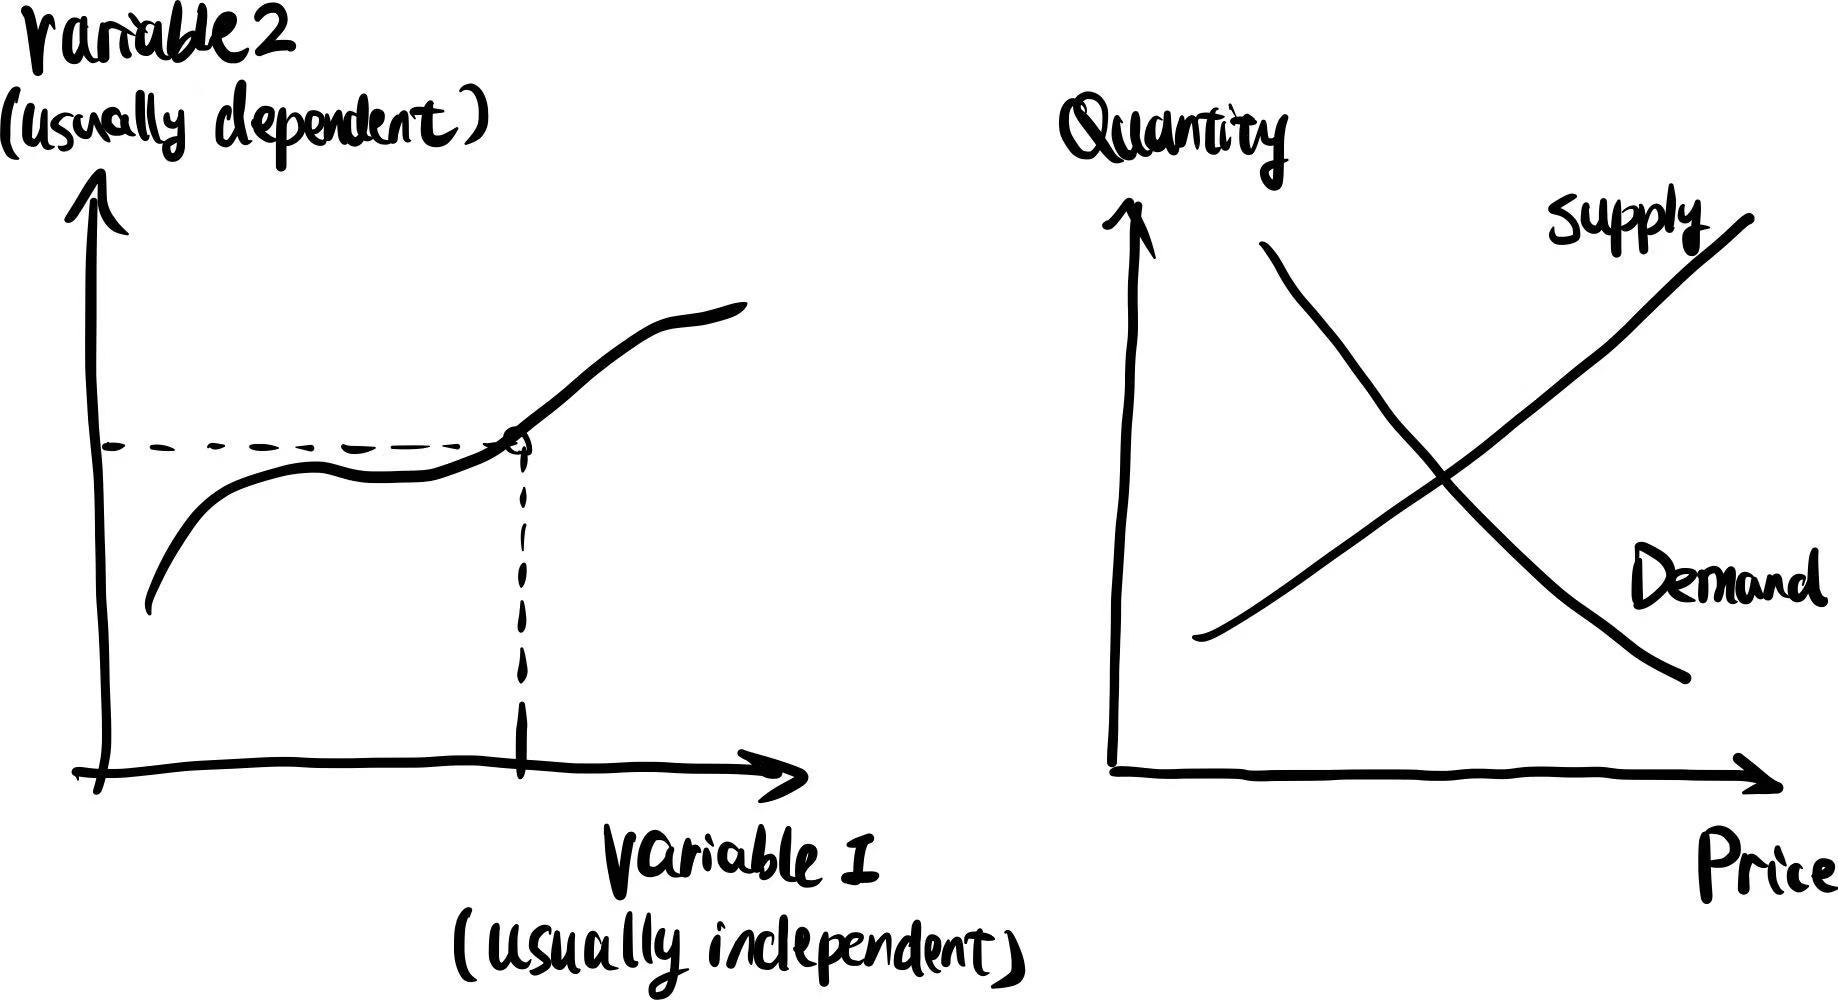
\includegraphics[width=0.9\textwidth]{img/image-20230228095149998.png}

\kaishu{\small 随着某商品的市场价格 (price) 增高, 生产者的生产意愿自然是增高的,
因为不考虑成本和其他因素变化的情况下 (Ceteris Paribus),
多生产的利润会更高, 因此供给曲线 (supply) 上扬, 反映出价格和供给量
(supply quantity) 的正相关; 另一方面,
消费者的消费意愿随着价格上涨自然是下降的, 于是需求曲线 (demand) 下压,
反映出价格和需求量 (demand quantity) 的负相关.

两条曲线分别对应着供给量和需求量关于价格的函数,
两函数的焦点反映了理想的自由市场下的最终成交价格和供需量
(因为在这个点达到了供需平衡 - equilibrium) ,
焦点向下作竖直线与横轴的焦点便显示了最终成交价格,
焦点向左作水平线与竖轴的交点便显示了平衡点的供需量.}
\end{tcolorbox}

在工程和计算机科学等思维里, 函数更像下左图所示, 给定一个输入 (input),
函数如同一台机器, 在加工后给出一个输出 (output); 这台机器非常可靠,
同样的输入能够稳定输出同样结果. 下右图给了一个例子

\begin{tcolorbox}[size=fbox, breakable, enhanced jigsaw]

\includegraphics[width=0.9\textwidth]{img/image-20230228095405809.png}

\kaishu{\small 假想有这样一个叫做``首都'' (Captital) 的函数,
放入一个国家名便会稳定输出这个国家的首都,
数学上我们可以这么标记下右图的例子 $\text{Capital(China)=Beijin}$.}
\end{tcolorbox}

函数的近现代定义和工科思维里的图景就很像, 考虑集合 $X$ 和 $Y$,
且它们不是空的, 如果存在某种特定的对应关系 $f$, 使得对于 $X$
中任意一个元素 $x$, 在 $Y$ 中都有唯一确定的元素 $y$ 和 $x$ 对应,
那么就称\textbf{映射} (mapping)\footnote{~Mapping 这个词用在这很贴切,
  map有地图的意思,
  ``映射''和地图上的每个点对应着实际区域上的一个个位置很相似.}
$f: A\rightarrow B$ 为从 $X$ 到 $Y$ 的一个函数, 记作
$y=f(x), x\in X$ 或者 $f(X)=\{y|f(x)=y, y\in Y\}$;
第一种记法强调元素的映射, 第二种记法强调整个集合的映射, $X$
在这里便是这个映射的定义域, $f(X)$ 是值域, $Y$
是这个映射的\textbf{陪域} (codomain, 也叫做上域, 到达域, 对应域),
大括号表示 $X$ 被映射到的集合, 其元素 $y$ 满足竖线后的条件, 即 $y$
是自 $x$ 通过 $f$ 这个映射得到, 并且 $y$ 属于 $Y$.
这样定义的直观感受类似下左图, 之前``首都''函数便类似下右图

\begin{tcolorbox}[size=fbox, breakable, enhanced jigsaw]
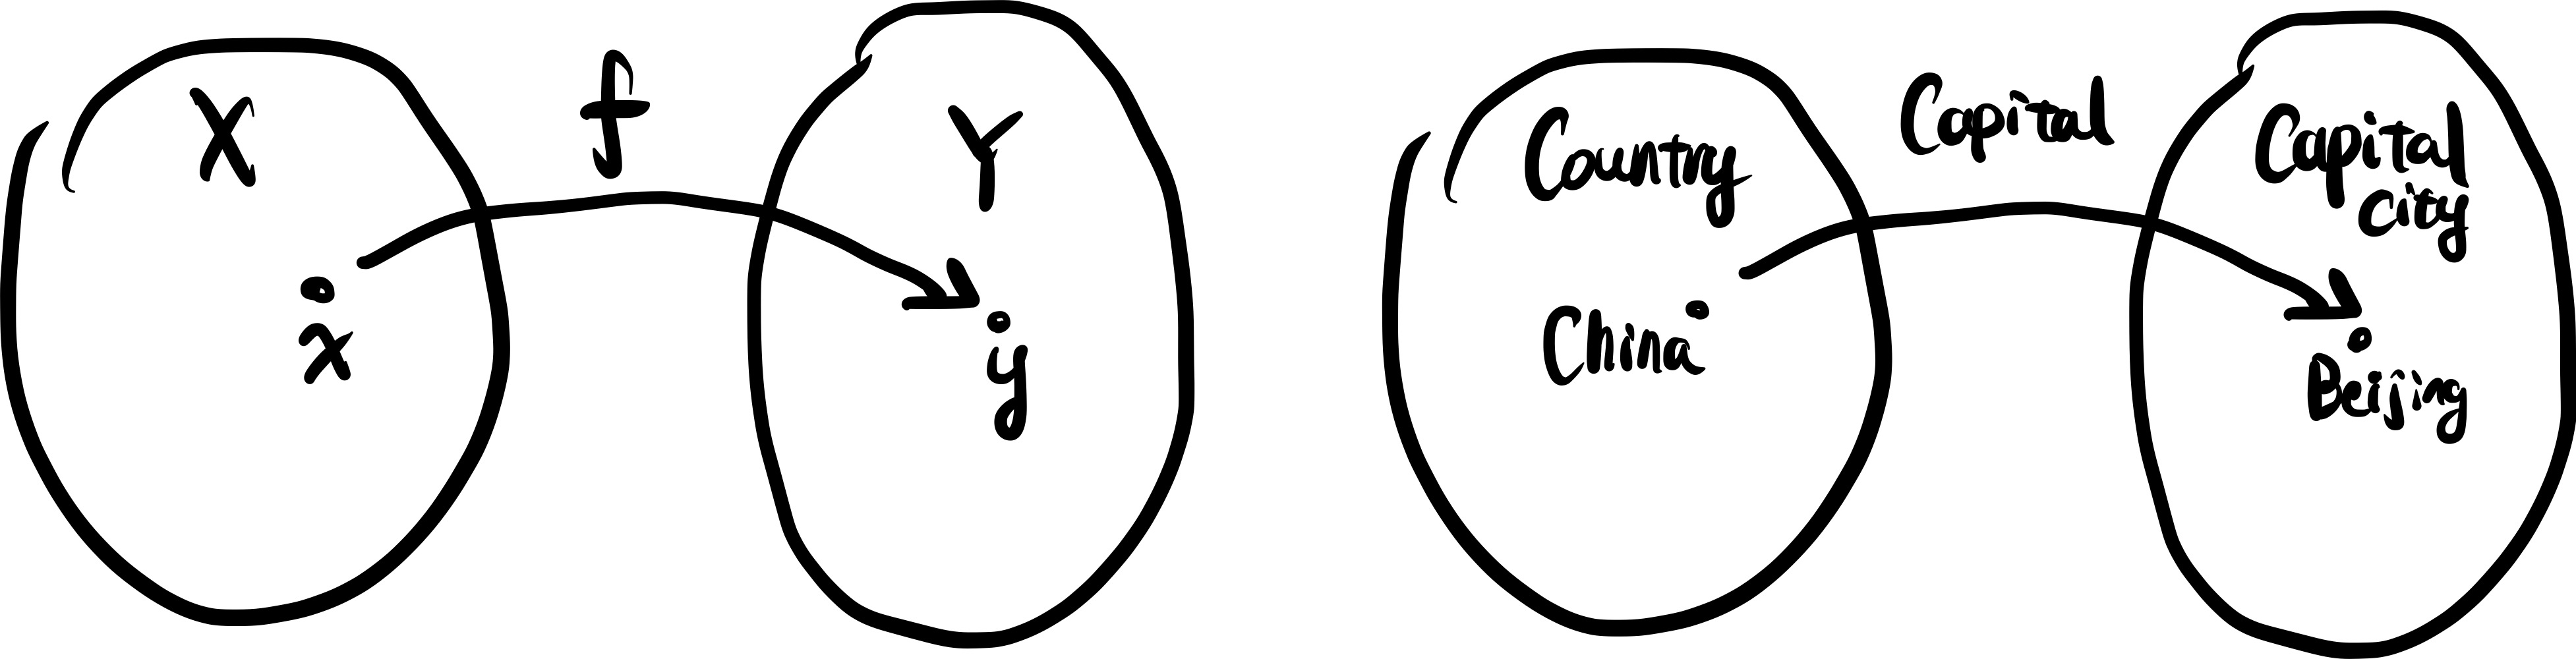
\includegraphics[width=0.9\textwidth]{img/image-20230228112941902.png}

\kaishu{\small Country这个集合里包含了很多国家, \{中国, 美国, 日本, \ldots\}; Capital
city这个集合里包含了很多城市, \{北京, 华盛顿, 东京, \ldots\};
Capital这个函数便描述了Country中的元素和Capital city中的元素的对应关系.}
\end{tcolorbox}

\end{tcolorbox}
%     \section{函数-下}\label{004}

\begin{flushright}{\kaishu 無名, 天地之始; 有名, 萬物之母. 常無, 欲以觀其妙; 常有, 欲以觀其徼. \\- 苏辙 『老子解』}\end{flushright}

\begin{tcolorbox}[size=fbox, breakable, enhanced jigsaw, title={单射, 满射, 双射 (injection, surjection,
bijection)}]

一个函数 $f:X\rightarrow Y$ 若满足, 如果 $a\neq b$ 则
$f(a)\neq f(b)$ 对于任何属于 $X$ 的 $a$ 和 $b$,
那么它便是\textbf{单射}的 (injection, one-to-one)\footnote{One-to-one
  是更``纯正''英语的说法, 比较通俗, injection 是来自法语的舶来词,
  更具高级感; 后面的 onto 和 surjection 同.}.

一个函数 $f:X\rightarrow Y$ , 若它的值域 (range) 和陪域 (codomain)
一致, 即对于任意 $y\in Y$, 都存在至少一个 $x\in X$ 满足
$f(x)=y$\footnote{介绍一下符号语言: $\exists$ - 存在; $\forall$ -
  对于所有. 于是这句话可以这么表述:
  $\forall y\in Y, \exists x\in X \text{ s.t. } f(x)=y$ (s.t.=such that
  可以译为``使得''). 但是通常情况下,
  还是尽量避免符号语言而使用自然语言来描述.}, 那么它便是\textbf{满射}的
(surjection, onto).

一个同时单射又满射的函数是\textbf{双射}的 (bijection, one-to-one
correspondance).

还是以Captial这个函数为例子, 下面给出了单射, 满射,
双射三种情况分别的图示:

\begin{tcolorbox}[size=fbox, breakable, enhanced jigsaw]
\begin{center}
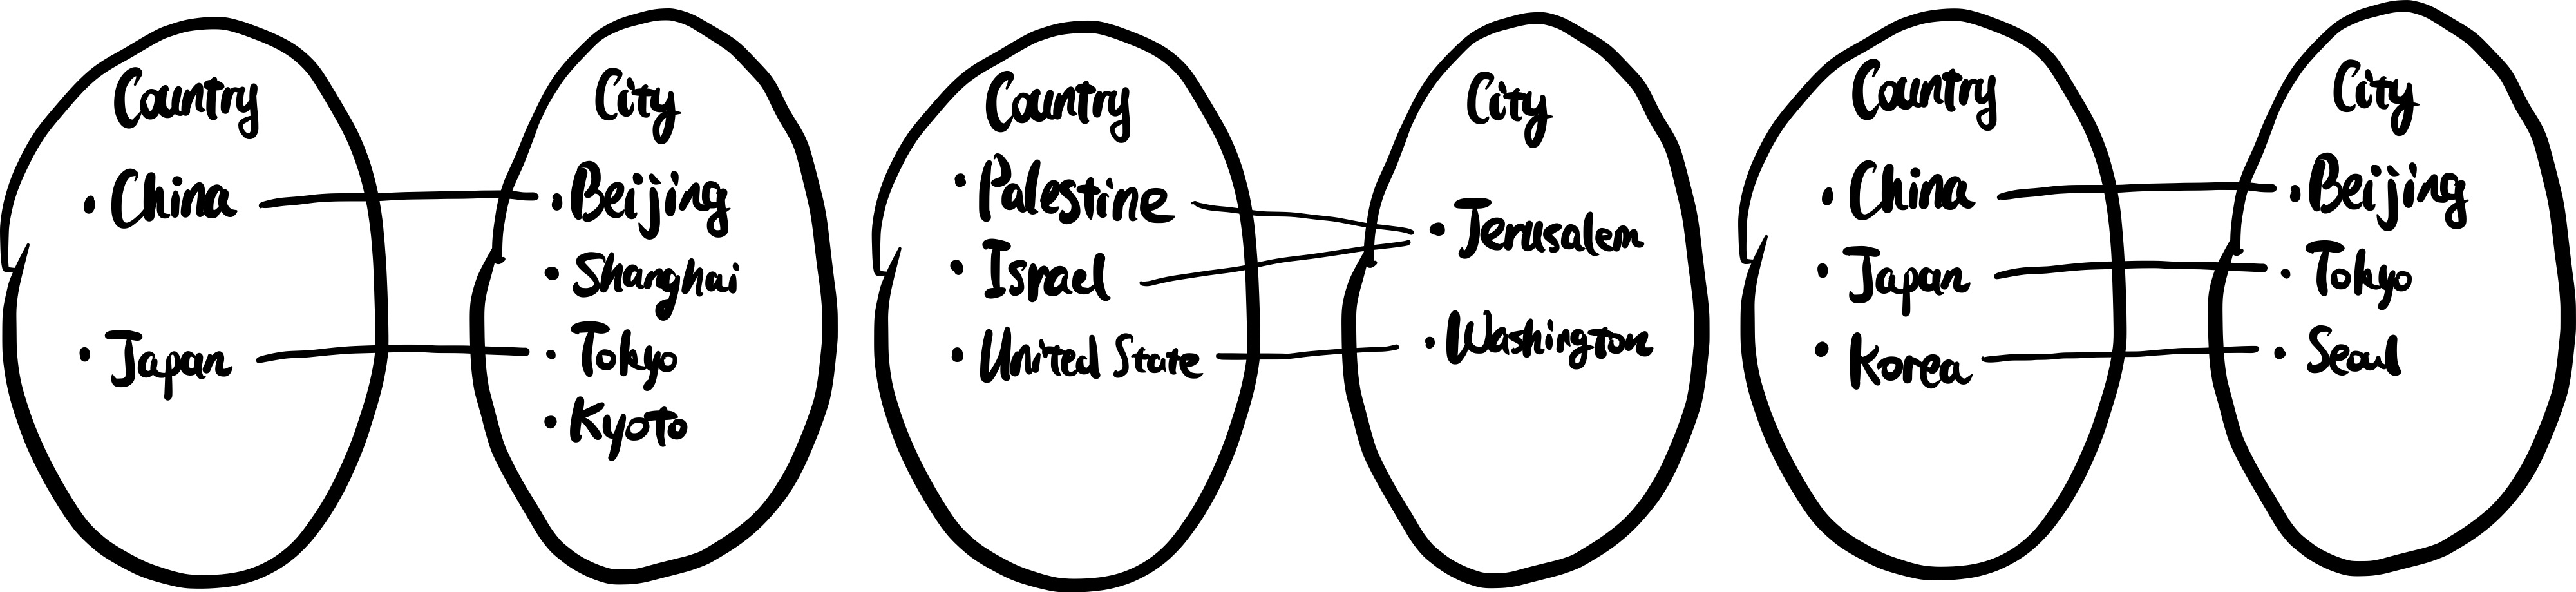
\includegraphics[width=0.9\textwidth]{img/image-20230302091706069.png}
\end{center}

\kaishu{\small 左: 单射但不满射; 中: 满射但不单射; 右: 双射.}
\end{tcolorbox}

\end{tcolorbox}

\begin{tcolorbox}[size=fbox, breakable, enhanced jigsaw, title={奇偶性 (parity 大嘘)}]

若一个函数满足 $f(-x)=-f(x)$, 即改变输入值 (自变量) 的正负号, 输出值
(因变量) 的正负号也改变, 这个函数便是\textbf{奇函数} (odd function).
图像上它是关于原点对称的.

若一个函数满足 $f(-x)=f(x)$, 即改变输入值 (自变量) 的正负号,
不影响输出值 (因变量) , 这个函数便是\textbf{偶函数} (even function).
图像上它是关于 $y$ 轴对称的.

当然, 奇函数和偶函数事实上是很特殊的两类函数,
更多的函数既不是奇函数又不是偶函数.

一些运算规律:

\begin{itemize}

\item
  奇函数 + 奇函数 = 奇函数\\{\kaishu 证明}: 假设存在两个奇函数 $f(x)$ 和
  $g(x)$, 令 $(f+g)(x) := f(x) + g(x)$, 即 $(f+g)(x)$
  这个函数是原本两函数之和. 根据奇函数的定义, $f(-x)=-f(x)$ 且
  $g(-x)=-g(x)$, 将两式相加得 $f(-x)+g(-x)=-f(x)-g(x)$, 即有
  $(f+x)(-x)=-(f+g)(x)$, 可见 $(f+g)(x)$ 是奇函数.
\item
  偶函数 + 偶函数 = 偶函数\\本条及接下来的证明与上一条类似, 可以当作练习.
\item
  奇函数 ×/÷ 奇函数 = 偶函数
\item
  偶函数 ×/÷ 偶函数 = 偶函数
\item
  奇函数 ×/÷ 偶函数 = 奇函数
\item
  偶函数 ×/÷ 奇函数 = 奇函数
\end{itemize}

\end{tcolorbox}

\begin{tcolorbox}[size=fbox, breakable, enhanced jigsaw, title={反函数 (inverse
function)}]

浅浅地非专业地叙述一下反函数. 设函数 $y=f(x)\ (x\in X)$ 的值域是
$Y$, 若存在一个函数 $g(y)$ 使得 $x= g(y)\ (y\in C)$, $g(x)$
便叫做 $f(x)$ 的\textbf{反函数} (inverse function), 可以记作
$x=f^{-1}(y)$, 它的定义域和值域分别是原函数的值域和定义域。

图像上, 反函数和原函数关于 $y=x$ 对称.

在求反函数时要特别注意反函数与原函数的定义域和值域. 例如 $y=f(x)=x^2$,
因为 $(\pm x)^2=y$, 反函数可能是 $x=f^{-1}(y)=\sqrt{y}$ 也可能是
$x=f^{-1}(y)=-\sqrt{y}$ , 但是不能是 $x=f^{-1}(y)=\pm\sqrt{y}$,
因为这样便不符合函数定义了, 一个输入值不可以有多个输出值,
或则说一个自变量不能对应多个因变量
(但是多个因变量对应一个自变量是允许的, 可以参考满射但不单射的图例).
这里反函数取正或负取决于原函数的定义域, 若 $y=f(x)=x^2, x\ge 0$, 则
$x=f^{-1}(y)=\sqrt{y}$; 若 $y=f(x)=x^2, x\le 0$, 则
$x=f^{-1}(y)=-\sqrt{y}$.

\end{tcolorbox}

\begin{tcolorbox}[size=fbox, breakable, enhanced jigsaw, title={隐函数 (implicit
function)}]

有的时候可能需要用函数来表达一个比较复杂的图像, 举一个简单一点的例子,
一个圆心位于原点的单位圆, 圆上任意一点到圆心距离都是 $1$, 于是有
$x^2+y^2=1$, 用前面学习的函数的形式表达这个关系, 有

$y=\begin{cases}\sqrt{1-x^2}\\-\sqrt{1-x^2}\end{cases}.$

这样似乎还没有起先的 $x^2+y^2=1$ 这个形式美观, 因此不妨还是用
$x^2+y^2-1=0$ 来表述单位圆上的 $x$ 与 $y$ 的关系. 类似这样,
利用一个【同时关于 $x$ 与 $y$ 的表达式 $F(x,y)=0$】来确定【 $y$
关于 $x$ 的函数】的表达式, 我们称之为\textbf{隐函数} (implicit
function); 为表区分, 前面介绍的类似 $y=f(x)$ 的函数,
称为\textbf{显函数} (explicit function).

\end{tcolorbox}

\begin{tcolorbox}[size=fbox, breakable, enhanced jigsaw, title={线性 (linearity)}]

这是一个很好的特性, 并不局限于函数, 仅对于函数来说的话,
若一个函数是线性的, 便有

$f(a+b)=f(a)+f(b),\ f(ax)=af(x).$

\end{tcolorbox}
%     \section{三角函数}\label{005}

\begin{flushright}{\kaishu 道可道, 非常道; 名可名, 非常名.}\end{flushright}

\begin{tcolorbox}[size=fbox, breakable, enhanced jigsaw, title={三角函数
(trigonometry)}]

三角函数最基本的使用应该是表示直角三角形的变长比. 如下图所示, 三角形
$ABC$ 为直角三角形, 将 $\angle BAC$ 记作 $\theta$, 对于两条直角边
$AB$ 和 $BC$, 边 $AB$ 在 $\theta$ 边上, 称它为\textbf{邻边}
(adjacent), 边 $BC$ 在 $\theta$ 对面, 称它为\textbf{对边}
(opposite), 剩余的边 $AC$ 被称为\textbf{斜边} (hypotenuse)。

\begin{tcolorbox}[size=fbox, breakable, enhanced jigsaw]
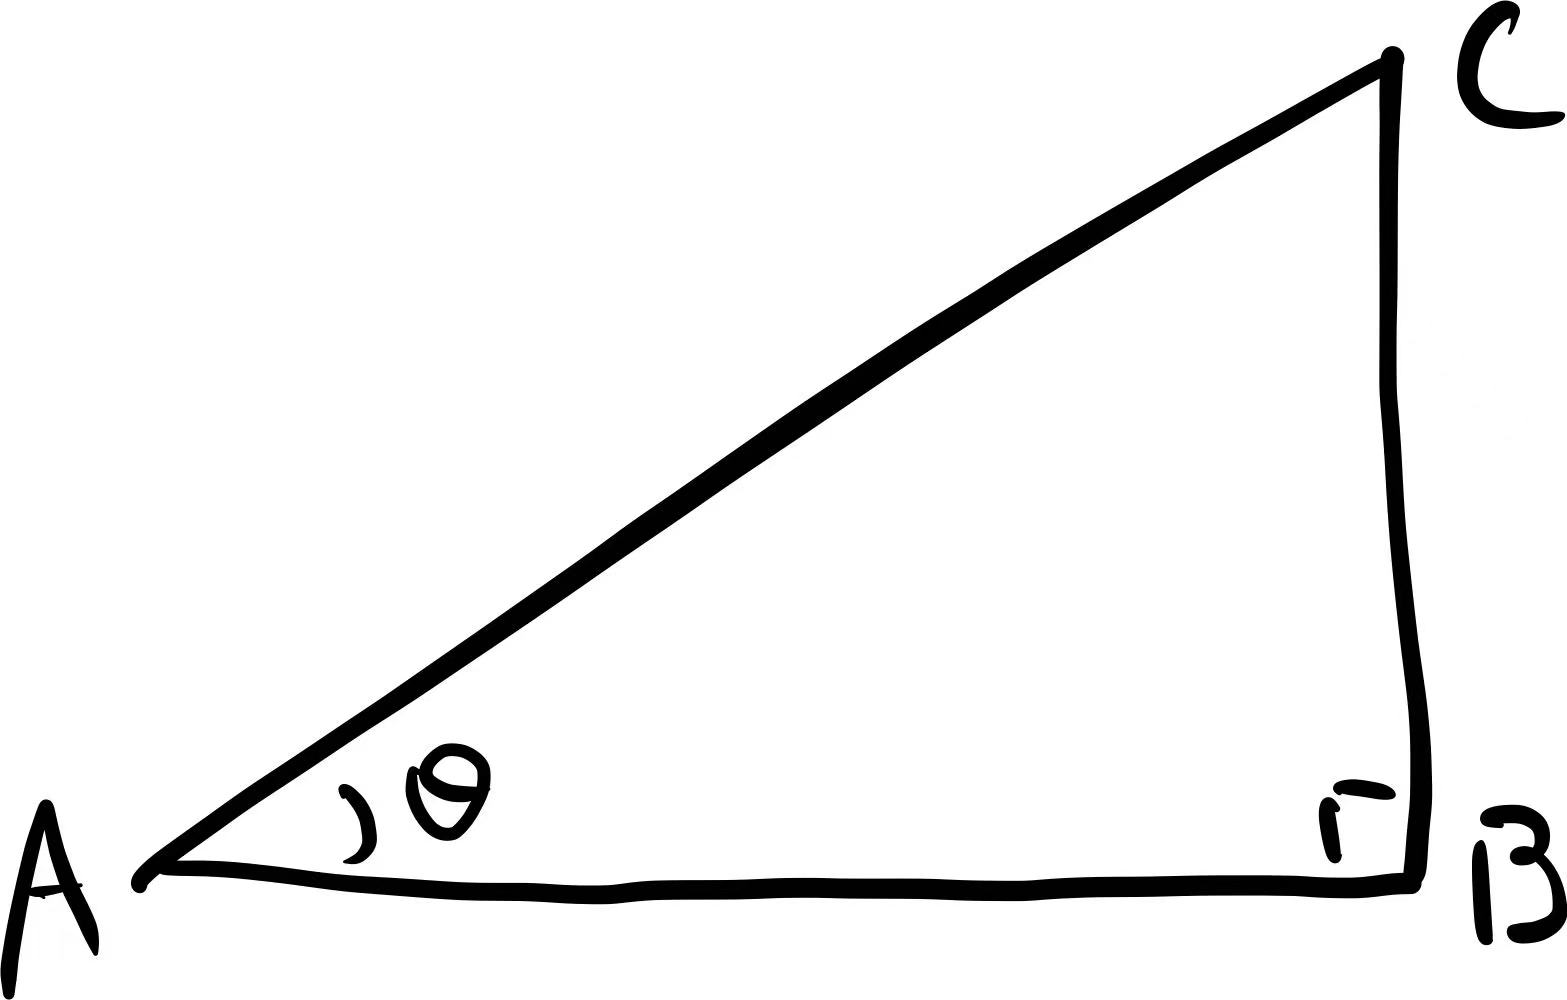
\includegraphics[width=0.5\textwidth]{img/image-20230308142717670.png}
\end{tcolorbox}

易见, 各变长比仅和 $\theta$ 相关\footnote{当然也可以说和除了直角外的另一个角
  $(90^\circ-\theta)$ 相关; 边长比可以通过一个除直角外的角确定是因为,
  除直角外另一角相等的直角三角形都相似, 它们的边长比是一致的。},
三角函数便是用来表示各个比例的, 常用的三角函数有

$\begin{aligned}\cos\theta&=\frac{\text{邻边}}{\text{斜边}}=\frac{AB}{AC},\\ \sin\theta&=\frac{\text{对边}}{\text{斜边}}=\frac{BC}{AC},\\ \tan\theta&=\frac{\text{对边}}{\text{邻边}}=\frac{BC}{AB}.\end{aligned}$

不难看出$\tan\theta=\frac{\sin\theta}{\cos\theta}$.

另外还有

$\begin{aligned}\sec\theta&\equiv\frac{1}{\sin\theta},\\ \csc\theta&\equiv\frac{1}{\cos\theta},\\ \cot\theta&\equiv\frac{1}{\tan\theta}.\end{aligned}$

$\csc$ 很多时候也记作 $\text{cosec}$.

一个非常实用的关系, 直角三角形中有\textbf{勾股定理} (Pythagorean
theorem): 斜边边长平方等于两直角边边长的平方之和, 即 $AC^2=AB^2+BC^2$;
两边同时除以 $AC^2$ 便有

\begin{itemize}

\item
  $\boxed{1=\cos^2\theta+\sin^2\theta}$.\footnote{三角函数的平方:
    cos(x)\textsuperscript{2} 通常理解为 cos((x)\textsuperscript{2});
    cos\textsuperscript{2}x 约定俗成表示 (cos(x))\textsuperscript{2}.}
\end{itemize}

\end{tcolorbox}

\begin{tcolorbox}[size=fbox, breakable, enhanced jigsaw, title={反三角函数}]

三角函数, 输入一个角度, 返回一个边长比; 反三角函数便是三角函数得逆运算,
或者说反函数 (参见【\ref{004}\nameref{004}】), 即输入一个边长比, 返回一个角度.

\end{tcolorbox}

\begin{tcolorbox}[size=fbox, breakable, enhanced jigsaw, title={正弦定律 (law of sine)}]

将三角形三个角分别记作 $\alpha$, $\beta$, 和 $\gamma$,
将它们的对边分别记作 $A$, $B$, 和 $C$. 先是结论:

\begin{itemize}

\item
  $\boxed{\frac{A}{\sin\alpha}=\frac{B}{\sin\beta}=\frac{C}{\sin\gamma}}$.
\end{itemize}

\begin{tcolorbox}[size=fbox, breakable, enhanced jigsaw]
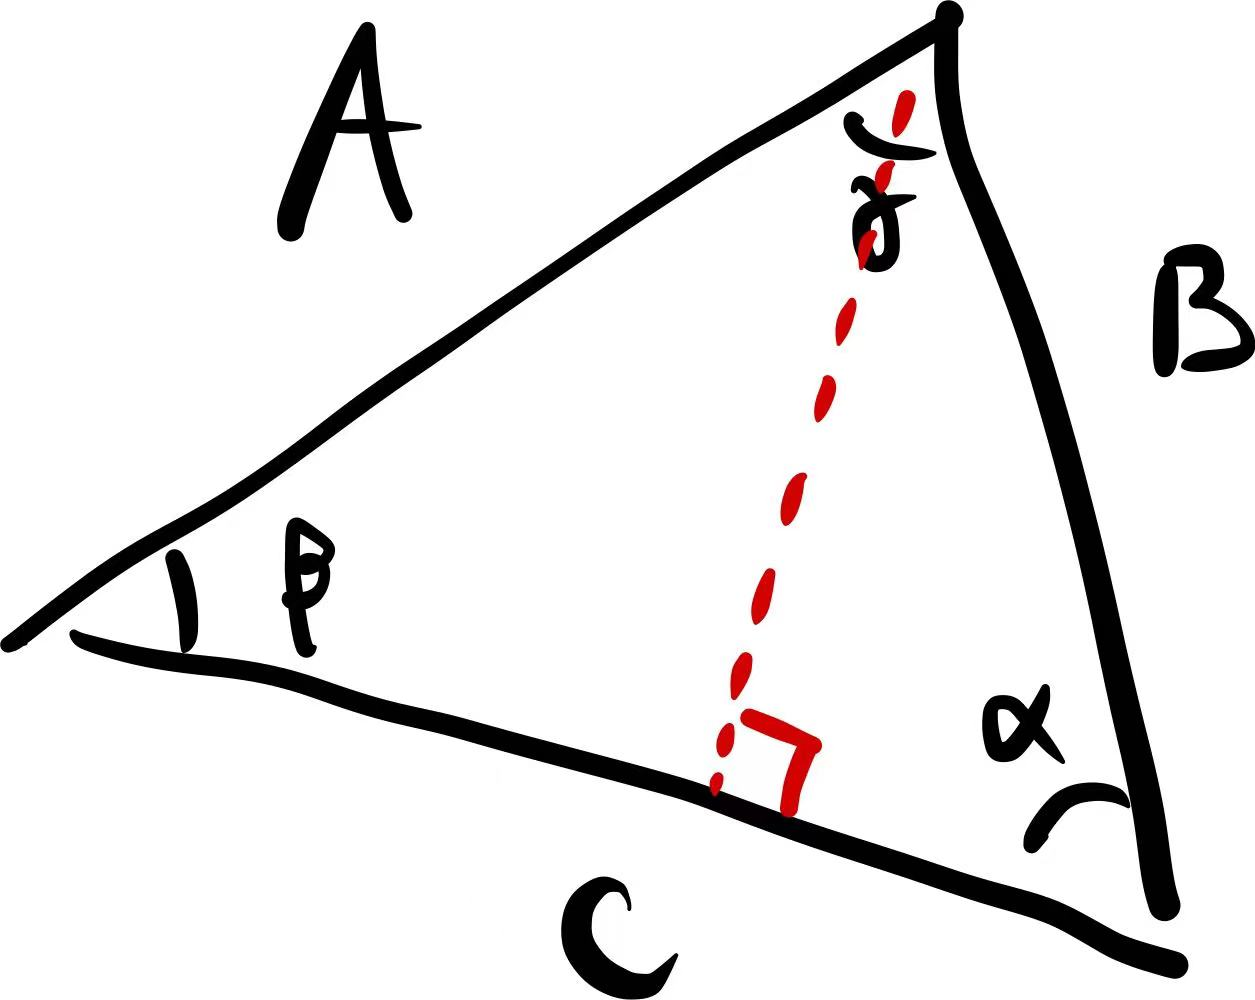
\includegraphics[width=0.5\textwidth]{img/image-20230308142913522.png}
\end{tcolorbox}

推导如下:

如上图所示, 以 $C$ 为底做高, 将原本的三角形分为左右两个直角三角形,
这条高利用左边的直角三角形可以表示为 $A\sin\beta$,
利用右边的直角三角形则是 $B\sin\alpha$, 于是有
$A\sin\beta=B\sin\alpha$, 整理可得
$\frac{A}{\sin\alpha}=\frac{B}{\sin\beta}$;
再做另一条高重复前面的操作, 便可得到完整的结论.

\end{tcolorbox}

\begin{tcolorbox}[size=fbox, breakable, enhanced jigsaw, title={余弦定律 (law of cosine)}]

还是先上结论:

\begin{itemize}

\item
  $\boxed{B^2=A^2+C^2-2AC\cos\beta}$,
\end{itemize}

即, 【一条边的边长平方】等于【另两条边的边长平方之】和加上【两倍的
(另两条边边长的乘积) 乘以 (另两条边的夹角的余弦)】.

\begin{tcolorbox}[size=fbox, breakable, enhanced jigsaw]
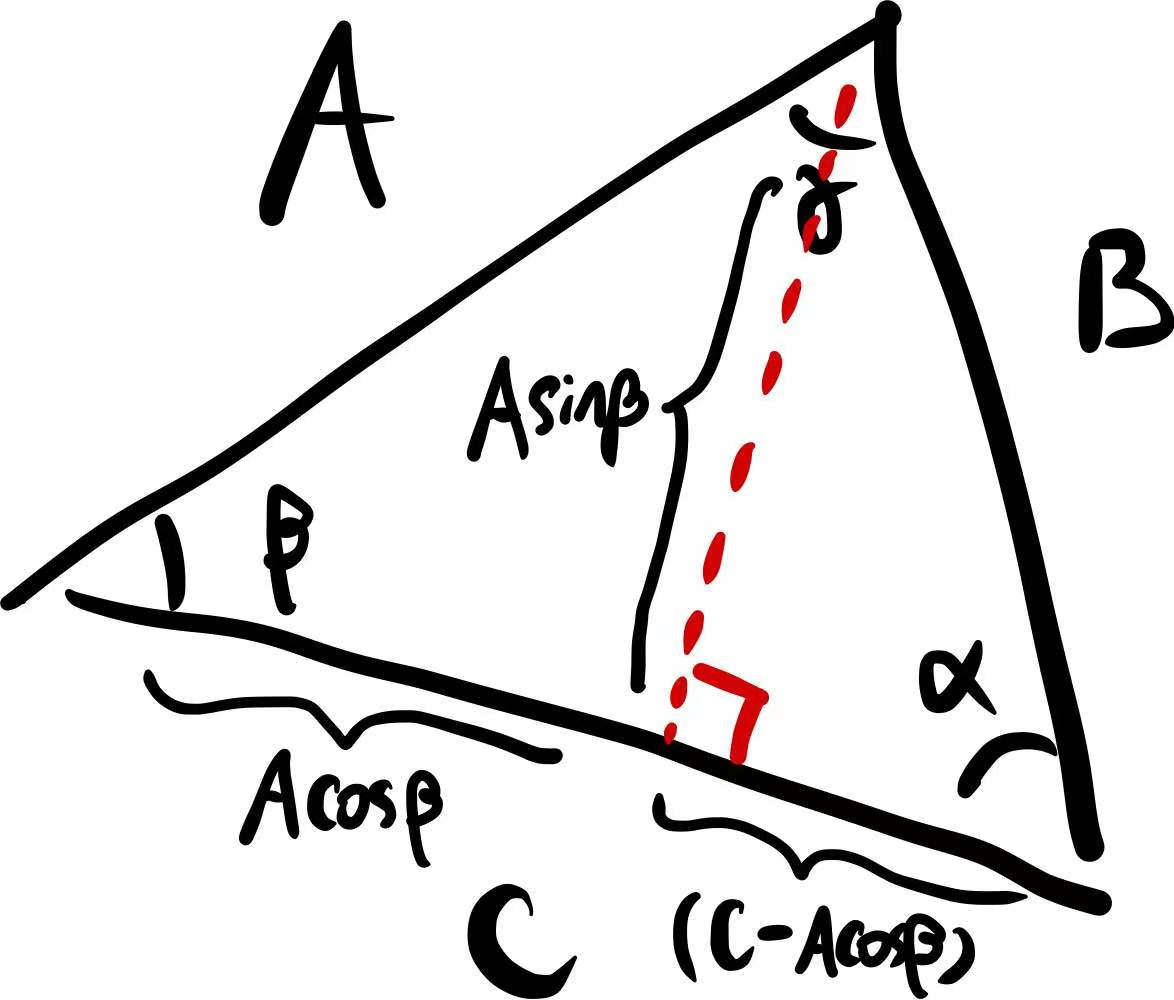
\includegraphics[width=0.5\textwidth]{img/image-20230308151417631.png}
\end{tcolorbox}

推导如下:

如下图所示, 依旧利用底边 $C$ 上的高将其分为左右两个直角三角形;
左边的直角三角形, 利用斜边 $A$ 和角 $\beta$, 两直角边分别可以表示为
$A\cos\beta$ 和 $A\sin\beta$, 于是右边的直角三角形边长便可表述为
$A\sin\beta$ 和 $(C-A\cos\beta)$; 对右边的直角三角形使用勾股定理

$\begin{aligned}B^2&=A^2\sin^2\beta+(C-A\cos\beta)^2\\ &=A^2\sin^2\beta+C^2+A^2\cos^2\beta-2AC\cos\beta\\ &=A^2+C^2-2AC\cos\beta.\end{aligned}$

其中等式的后两行用到了之前得出的 $1=\cos^2\theta+\sin^2\theta$.

\end{tcolorbox}

\begin{tcolorbox}[size=fbox, breakable, enhanced jigsaw, title={任意角度的三角函数}]

不难发现, 前面讨论的情况似乎都是锐角的情况 (主要是因为插图\ldots),
钝角的三角函数似乎没那么直观了, 因为做不成一个含有钝角的直角三角形,
没法简单地用边长比来表示 $\sin$ 和 $\cos$ 等. 于是,
我们需要想办法将前面的情形推广.

如下左图所示, 建立直角坐标系, 做一圆心位于原点的单位圆, 即半径为 $1$
的圆, 考虑在第一象限的圆上的一点, 将其与原点做连线, 将从
$x$-轴正方向与这条连线\textbf{顺时针}方向形成的夹角记作 $\theta$,
不难看出这个点的坐标 $(x,y)$ 满足

$\begin{cases}x=\cos\theta,\\y=\sin\theta.\end{cases}$

\begin{tcolorbox}[size=fbox, breakable, enhanced jigsaw]
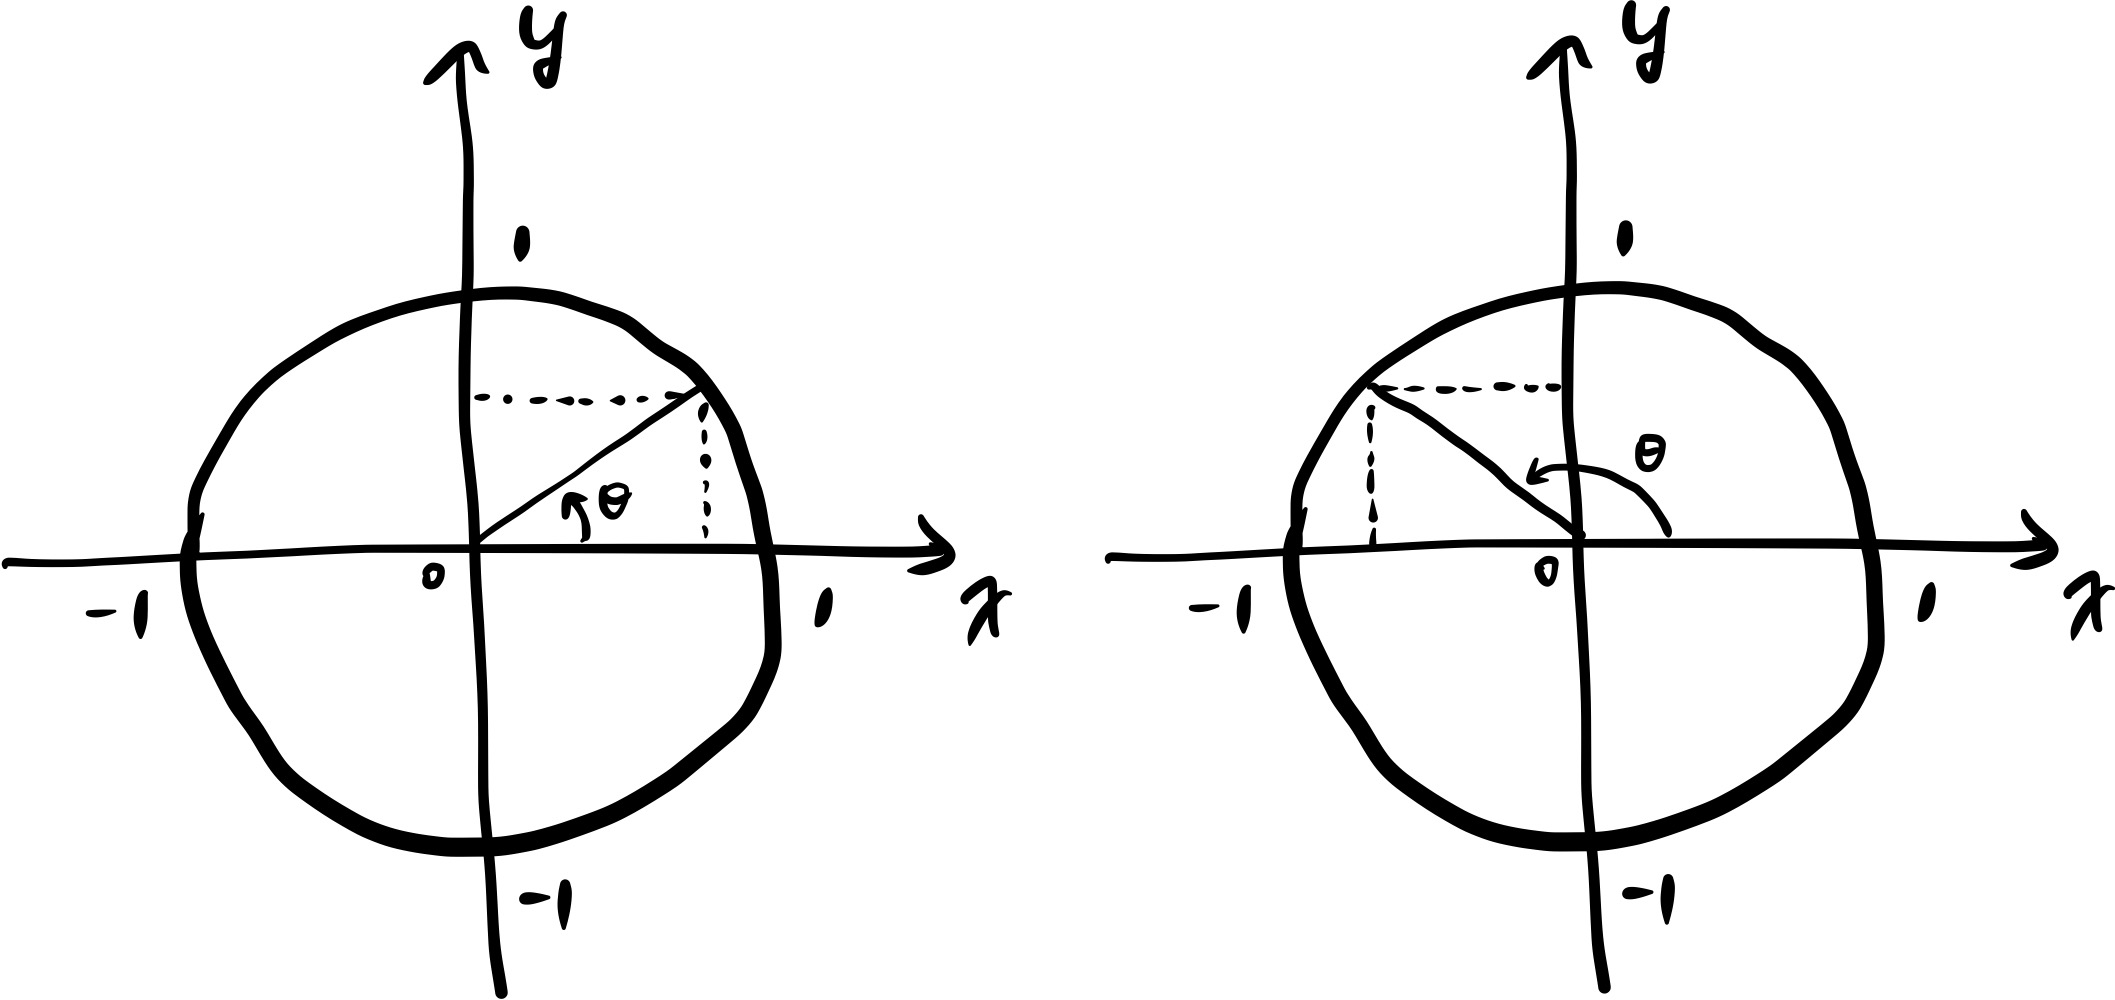
\includegraphics[width=0.75\textwidth]{img/image-20230316171124433.png}
\end{tcolorbox}

于是不妨将其他象限的情况也按此定义,
于是如上右图所示的钝角甚至更大角度的三角函数便可以被定义了.

\end{tcolorbox}

\begin{tcolorbox}[size=fbox, breakable, enhanced jigsaw, title={弧度制 (radian)}]

为什么一个周角是 $360^\circ$ 呢, 听说过一个不可考的说法: $360$
是一个有很多因数的数字 (1, 2, 3, 4, 5, 6, 8, 9, 10, 12\ldots),
等分起来的时候数字会比较友好, 所以 $360^\circ$ 其实是非常随意地规定的.
那么有没有更好的用来描述角度方法呢? 答案是弧度.

一个半径为 $r$ 的圆的周长是 $2\pi r$, 一个圆心角为 $n^\circ$
的扇形的弧长是 $2\pi r\frac{n}{360}$. 可见圆心角越大弧越长,
且圆心角和弧长成正比. 既然如此,
不如重新将角度定义为圆心角与弧长的比值以方便计算, 于是便有了,
在新的这套单位系统中, 若圆心角大小为 $\theta$, 其对应弧长应为
$r\theta$; 当圆心角是一个周角时, 对应弧长便成了圆的周长 $r(2\pi)$.
所以角度和这个新的单位的换算有 $360^\circ\equiv 2\pi\ \text{rad}$,
因为这个单位把圆心角和对应的弧长联系起来了, 因此称之为\textbf{弧度}
(radian).

扇形面积在这套单位制, 即弧度制下, 便也成了 $\frac{1}{2}r^2\theta$.

\end{tcolorbox}

\begin{tcolorbox}[size=fbox, breakable, enhanced jigsaw, title={三角函数的图像}]

现在这个时代, 大家都或多或少能接触到科学计算器,
再不济在bing.com上搜索``solver''用微软的 Microsoft Solver
也可以计算某个特定角度的三角函数值, 自然也可以绘制函数图像.
下图分别展示了 $\sin(x)$ 和 $\cos(x)$ 的图像,

\begin{tcolorbox}[size=fbox, breakable, enhanced jigsaw]
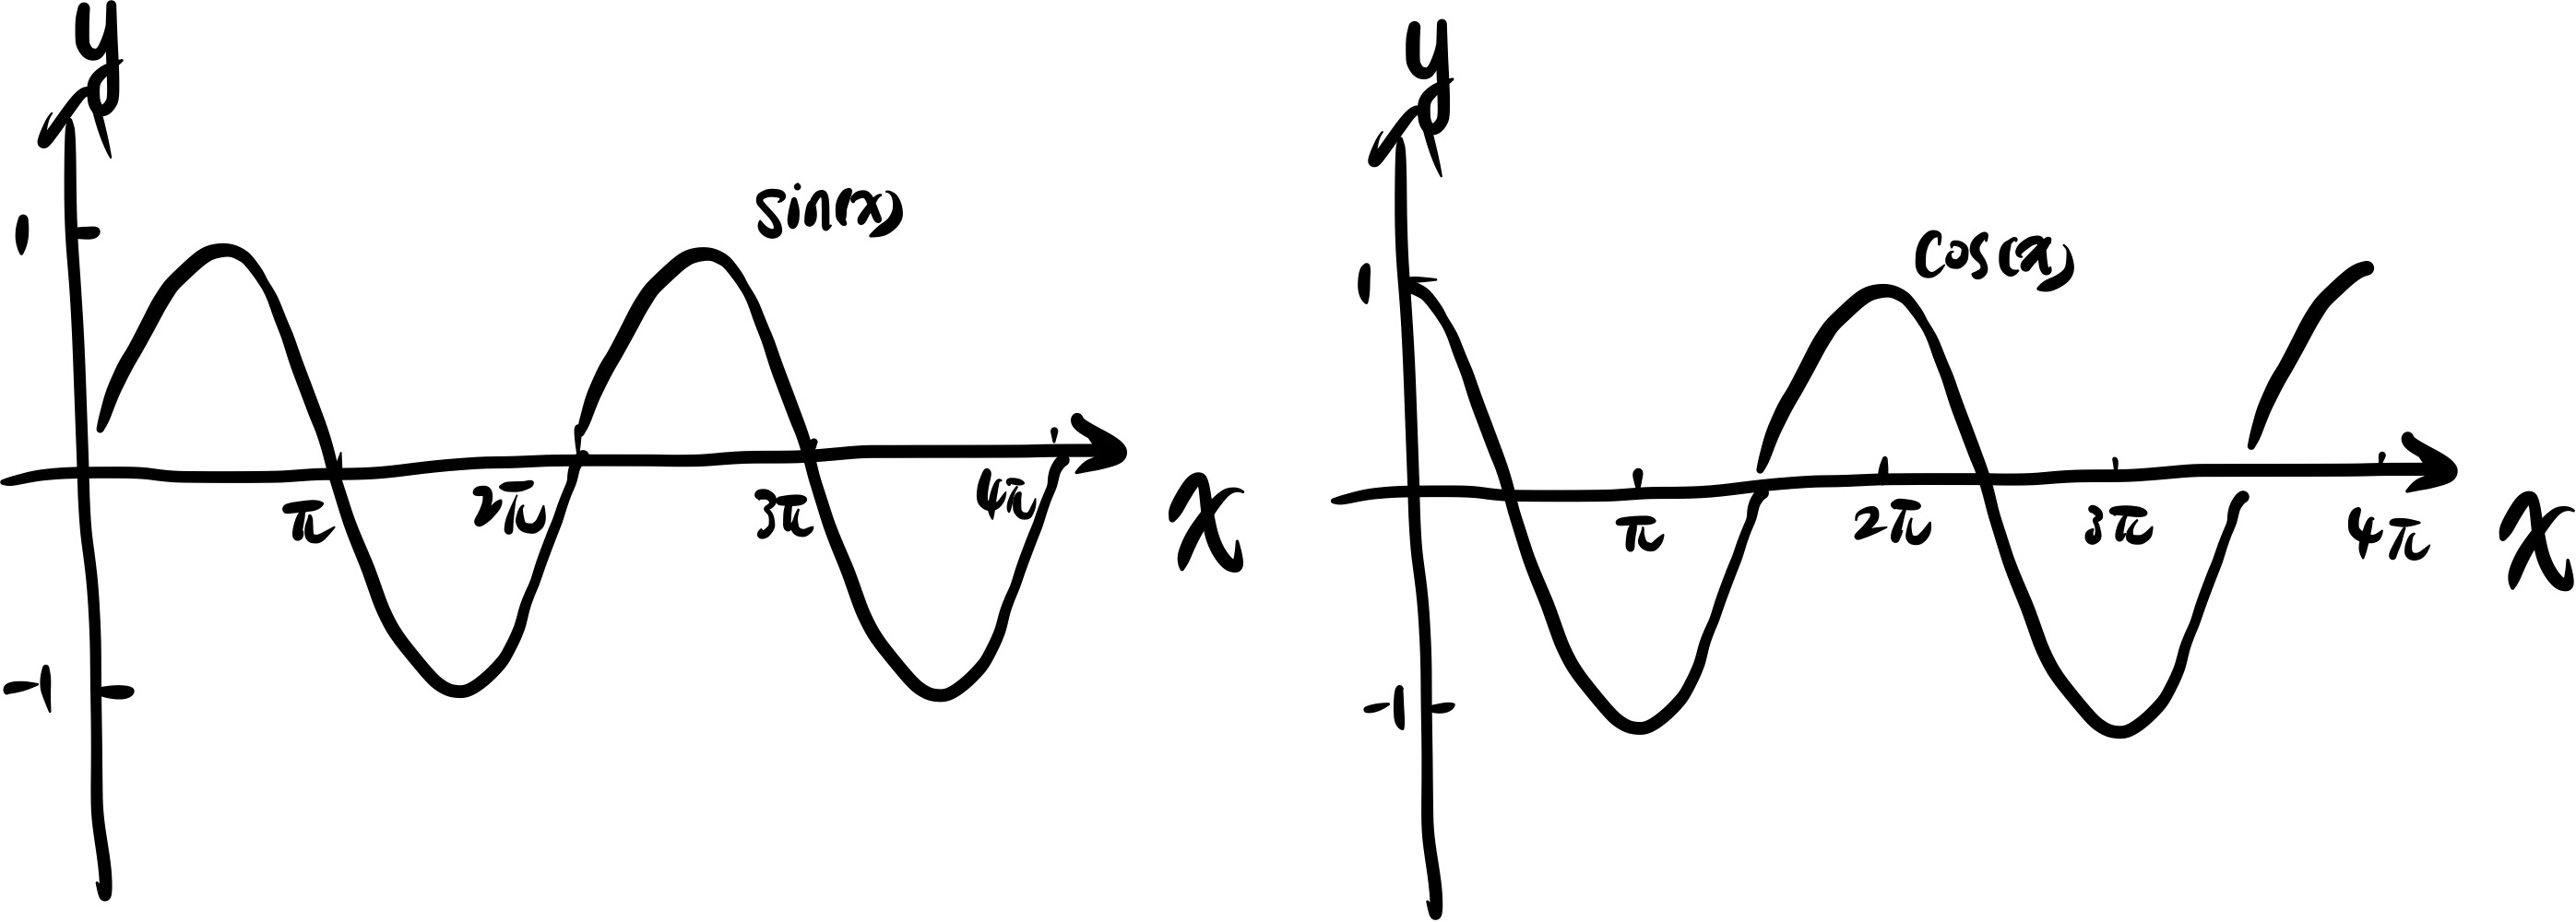
\includegraphics[width=0.75\textwidth]{img/image-20230316171137500.png}
\end{tcolorbox}

一些值得关注的点是它们都是\textbf{周期函数} (periodic function),
随着自变量-角度的变化, 因变量-函数值的变化是周期性的, 它们的周期都是
$2\pi$, 这一点从上文的单位圆里便可看出些许原因,
当角度变化超过一个周角时, 和角度刚从 $0$ 开始的情况是一样的.

\end{tcolorbox}
%     \section{虚数和复数}\label{006}

\begin{flushright}{\kaishu 些许绕行 (detour).}\end{flushright}

\begin{tcolorbox}[size=fbox, breakable, enhanced jigsaw, title={虚数和复数 (imaginary number and complex number)}]

考虑一个一元二次方程 $ax^2+bx+c=0$, 它的解有

$\begin{aligned}
0&=a\left(x^2+\frac{b}{a}x+\frac{c}{a}\right)\\
0&=x^2+\frac{b}{a}x+\frac{c}{a}\\
0&=x^2+\frac{b}{a}x+\left(\frac{b}{2a}\right)^2-\left(\frac{b}{2a}\right)^2+\frac{c}{a}\\
0&=\left(x-\frac{b}{2a}\right)^2-\left(\frac{b}{2a}\right)^2+\frac{c}{a}\\
\left(x-\frac{b}{2a}\right)^2&=\left(\frac{b}{2a}\right)^2-\frac{c}{a}\\
&...\\
x&=\boxed{\frac{-b\pm\sqrt{b^2-4ac}}{2a}}.
\end{aligned}$

上式最后的结论便是求根公式, 不难看出整个推导过程实际上就是配方,
其中根号前面的``加减''是因为对等式两边同时开方时,
正负两种情况都是正确的.

我们在此之前接触到的数字都还限于实数范围内, 因此会要求
$\left(b^2-4ac\right)$ 是正的, 以保证开方之后的结果是``有意义的'',
然而

\begin{newquote}
    ``从来如此, 便对么?''
\end{newquote}

之前也出现了, 不能被表示成分数形式的数字,
我们的研究范围从有理数扩充到了实数; 现在, 若 $\left(b^2-4ac\right)$
是负的, 按照当前的理解, 它不能被开方, 那是不是又到了这样一个神圣的时刻,
我们需要拓展我们研究的数字的范围?

既然如此, 不如规定 $\sqrt{-1}\equiv i$, 作为新的一类数字的单位,
因为之前的数字叫``实数'', 那么这一类新的数字就不妨叫做``\textbf{虚数}''
(imaginary number) 吧. 一个既包含实数部分, 又包含虚数的部分的数字,
我们就叫它``\textbf{复数}'' (complex number), 记作 $\mathbb{C}$.
\end{tcolorbox}

\begin{tcolorbox}[size=fbox, breakable, enhanced jigsaw, title={运算规律}]

考虑若干个复数, $z_1=a+bi$, $z_2=c+di$, $z_3=e+fi$\ldots{}

\begin{itemize}

\item
  \textbf{加法}: $z_1+z_2=(a+c)+(b+d)i$.
  实数部分和虚数部分可以分开计算,
  应该不难看出复数和加法是构成\textbf{阿贝尔群}的
  (即它具有封闭性和结合律, 有单位元和逆元, 并且有交换律, 详细参见\ref{001}\nameref{001}).
\item
  \textbf{乘法}:
  $z_1\times z_2=(a+bi)\times(c+di)\\=ac+adi+bci+bdi^2=(ac-bd)+(ad+bc)i.$
  不难看出, 复数和乘法也构成阿贝尔群.
\item
  乘法对于加法满足\textbf{分配律}, 即,
  $(z_1+z_2)\times z_3=z_1\times z_3+z_2\times z_3$,
  证明留作练习\footnote{事实上, 很多情况下, 之前提到的很多知识点,
    例如单位元, 零元, 逆元都分左右, 分配律也有左分配律和右分配律,
    但是目前讨论的情况都是满足交换律的, 所以可以不区分左右.}.
\end{itemize}

以上三条已经足够使得复数与加法和乘法构成一个\textbf{环} (ring), 事实上,
环只需要乘法是半群 (semi-group, 即满足结合律和有单位元的二元运算与集合) 即可.

\begin{itemize}

\item
  \textbf{减法}: 因为加法存在逆元, 所以减去一个数,
  可以视作加上这个数的加法逆元, 即:
  $z_1-z_2=(a+bi)-(c+di)\\\Rightarrow z_1+(-z_1)=(a+bi)+(-(c+di))=(a-c)+(b-d)i$
\item
  \textbf{除法}: 不难发现每个非零的元素都有乘法逆元,
  因此除以一个数可以视作乘上这个数的乘法逆元, 即: 因为
  $z_2\times\frac{1}{z_2}=\frac{c+di}{c+di}=1$, 于是
  $z_1\div z_2=z_1\times\frac{1}{z_2}=\frac{a+bi}{c+di}$.
\end{itemize}

\begin{newquote}
一点小插曲, $\frac{a+bi}{c+di}$ 应该怎么化简呢,
怎么写成简单的实数部分加上虚数部分的形式呢?
回顾一下无理数的``分母有理化'', 例如有
$\frac{a+\sqrt{b}}{c+\sqrt{d}}$, 我们会将分子分母同时乘以
$(c-\sqrt{d})$ 将分母变为有理数, 便有
$\frac{(a+\sqrt{b})(c-\sqrt{d})}{c^2-d}$. 类似的, 当我们尝试化简
$\frac{a+bi}{c+di}$时, 我们也不妨对分子分母同时乘以 $(c-di)$, 于是有
$\frac{(a+bi)(c-di)}{c^2+d^2}$, 分母便变为了实数,
再稍加化简便可转化为一个实数加上一个虚数的形式. 我们称 $(c-di)$ 是
$(c+di)$ 的\textbf{复共轭} (complex conjugate)\footnote{两头牛背上的架子称为轭,
  轭使两头牛同步行走. 共轭就描述了两个对象这样一种相生相随的关系.}.
\end{newquote}

像上述这样可以进行加减乘和除零外除法,
并满具足一些特定的阿贝尔群的特点和分配律的代数结构,
换言之一个满足交换律的环 (交换环 commutative ring)
附加上除零外元素的除法运算, 构成一个\textbf{域} (field), 可以记作
$\mathbb{F}$, 常见的例子有有理数域, 实数域, 复数域.

\begin{tcolorbox}[size=fbox, breakable, enhanced jigsaw]
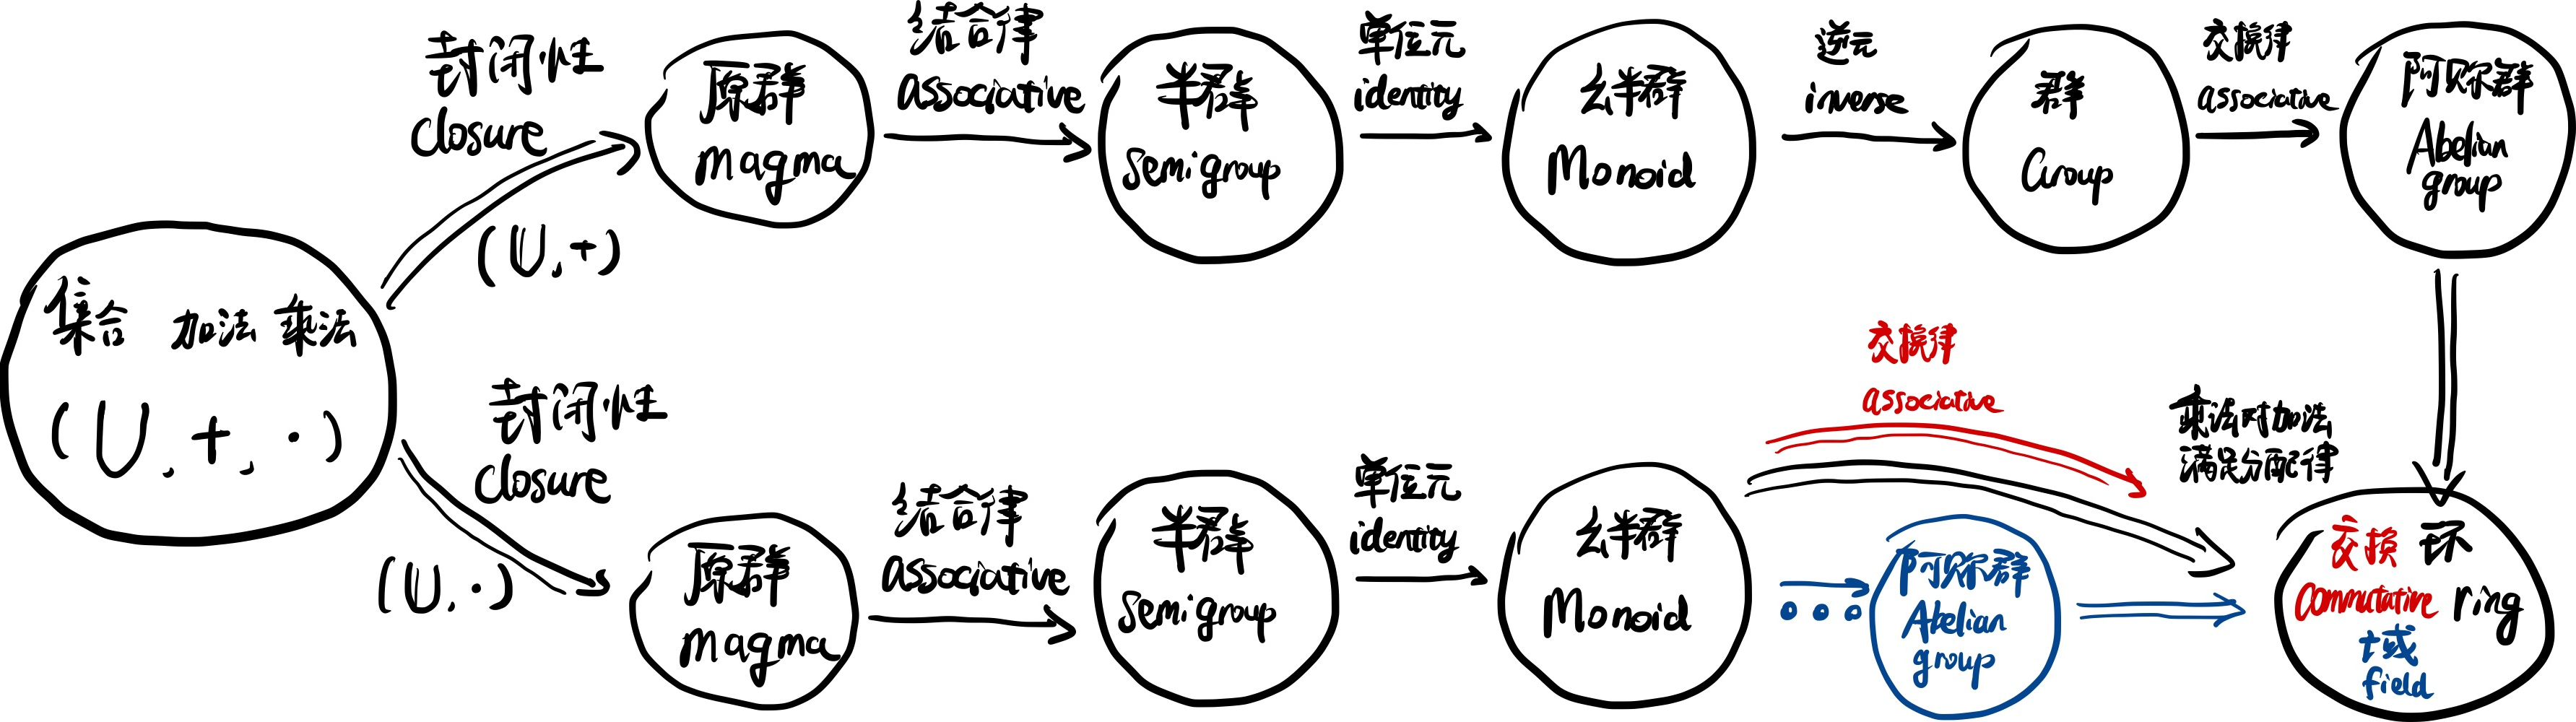
\includegraphics[width=0.9\textwidth]{img/image-20230328100716650.png}

\kaishu{\small 环, 交换环, 域的关系, 图改自知乎@SparkAndShine}
\end{tcolorbox}

\end{tcolorbox}
%     \begin{quote}
绕行之绕行 (detour of the detour).
\end{quote}

\hypertarget{ux4e8cux9879ux5f0fux5c55ux5f00-binomial-expansion}{%
\subsubsection{二项式展开 (binomial
expansion)}\label{ux4e8cux9879ux5f0fux5c55ux5f00-binomial-expansion}}

\textbf{二项式展开}指的是将类似 \((x+y)^n\) 的表达式展开的过程. 结论上有

\(\boxed{(x+y)^n=\sum_{r=0}^n\binom{n}{r}x^{n-r}y^r}.\)

这里 \(\binom{n}{r}=\frac{n!}{r!(n-r)!}\) 也记作 \(_nC_r\),
这个''C''是\textbf{组合} (combination) 的意思, 其中又有
\(n!=n\times(n-1)\times...\times3\times2\times1\).

\begin{quote}
上面第一次出现了求和符号 \(\sum\), 在此用一些例子说明,

\(\sum_{i=1}^{10}i=1+2+3+...+9+10;\)

\(\sum_{x=1}^{10}x^2=\left.x^2\right|_{x=1}+\left.x^2\right|_{x=2}+...+\left.x^2\right|_{x=10}=1^2+2^2+...+10^2.\)

即, 求和符号后的表达式, 依次代入求和符号下方的值,
符号下方的值加一\ldots, 直至代入求和符号上方的值, 最后将这些项求和.
\end{quote}

二项式展开的证明思路如下:

\textbf{从组合的思路出发}

\begin{itemize}
\item
  将 \((x+y)^n=\underbrace{(x+y)(x+y)...(x+y)}_{n}\) 展开,
  并将同类项合并, 易见可能出现的项的形式仅为 \(x^n=x^ny^0\),
  \(x^{n-1}y=x^{n-1}y^1\), \(x^{n-2}y^2\), \ldots{} \(x^2y^{n-2}\),
  \(xy^{n-1}=x^1y^{n-1}\), \(y^n=x^0y^n\).
\item
  合并后这些项的系数是合并前它们分别出现的次数,

  \begin{itemize}
  \tightlist
  \item
    \(x^n\) 相当于展开时每一个 \((x+y)\) 都选取 \(x\) 的情况,
    只有一种这样的情况, 即合并前 \(x^n\) 只可能出现 \(1\) 次,
    那么合并后它的系数便是 \(1\).
  \item
    \((x^{n-1}y^1)\) 相当于展开时每一个 \((x+y)\) 选取了 \((n-1)\) 个
    \(x\) 和 \(1\) 个 \(y\), 利用组合学的知识有
    \(n=\frac{n!}{1!(n-1)!}\) 种这样的情况, 即合并前 \((x^{n-1}y^1)\)
    出现 \(n\) 次, 那么合并后它的系数便是 \(n\).
  \end{itemize}

  \begin{quote}
  这个 \(n\) 可以这么看待, 选取的这个 \(y\) 可以出自这 \(n\) 项
  \((x+y)\) 中的任意一个, 于是便有 \(n\) 种可能.
  \end{quote}

  \begin{itemize}
  \tightlist
  \item
    \((x^{n-2}y^2)\) 相当于展开时每一个 \((x+y)\) 选取了 \((n-2)\) 个
    \(x\) 和 \(2\) 个 \(y\), 利用组合学的知识有
    \(\frac{n(n-1)}{2!}=\frac{n!}{1!(n-1)!}\) 种这样的情况, 即合并前
    \((x^{n-1}y^1)\) 出现 \(n\) 次, 那么合并后它的系数便是 \(n\).
  \end{itemize}

  \begin{quote}
  这个 \(\frac{n(n-1)}{2!}\) 可以这么看待, 选取的这两个 \(y\) 可以出自这
  \(n\) 项 \((x+y)\) 中的任意两个, 第一个 \(y\) 有 \(n\) 种选法,
  第二个因为第一个''占用''了一个 \((x+y)\), 因此它只有 \((n-1)\) 种选法,
  综上便有了 \(n(n-1)\); 然后两个 \(y\) 的顺序是无所谓的, 两个 \(y\)
  本身先后的排序会额外引入一个倍数 \(2\), 于是除掉.
  \end{quote}

  \begin{itemize}
  \tightlist
  \item
    \ldots{}
  \item
    \((x^{n-r}y^r)\) 相当于展开时每一个 \((x+y)\) 选取了 \((n-r)\) 个
    \(x\) 和 \(r\) 个 \(y\), 利用组合学的知识有
    \(\frac{n(n-1)...(n-r)}{(n-r)!}=\frac{n!/r!}{(n-r)!}=\frac{n!}{1!(n-1)!}=\binom{n}{r}\)
    种这样的情况, 即合并前 \((x^{n-1}y^1)\) 出现 \(\binom{n}{r}\) 次,
    那么合并后它的系数便是 \(\binom{n}{r}\).
  \end{itemize}

  \begin{quote}
  这个 \(\frac{n(n-1)...(n-r)}{(n-r)!}\) 可以这么看待, 选取的这 \(r\) 个
  \(y\) 可以出自这 \(n\) 项 \((x+y)\) 中的任意 \(r\) 个, 第一个 \(y\) 有
  \(n\) 种选法, 第二个因为第一个''占用''了一个 \((x+y)\), 因此它只有
  \((n-1)\) 种选法, 第三个于是只有 \((n-2)\) 种\ldots{} 综上便有了
  \(n(n-1)...(n-r)\); 然后 \(r\) 个 \(y\) 的顺序是无所谓的, \(r\) 个
  \(y\) 本身先后的排序, 第一个 \(y\) 顺序可能是 \(1\) 至 \(r\), 有 \(r\)
  种选择, 第二个只有 \((r-1)\)\ldots{} 于是会额外引入一个倍数
  \(r(r-1)...1=r!\), 于是除掉.
  \end{quote}
\item
  可见某一项 \((x^{n-r}y^r)\), 系数应为 \(\binom{n}{r}\), \(r=0\) 至
  \(r=n\) 的项都是允许的, 于是利用求和符号表示, 便有了最开始的结论.
\end{itemize}

这样的思路也可以推出杨辉三角 (Pascal's Triangle):

\begin{Shaded}
\begin{Highlighting}[]
    \FloatTok{1}
   \FloatTok{1}  \FloatTok{1}
  \FloatTok{1}  \FloatTok{2}  \FloatTok{1}
 \FloatTok{1}  \FloatTok{3}  \FloatTok{3}  \FloatTok{1}
\FloatTok{1}  \FloatTok{4}  \FloatTok{6}  \FloatTok{4}  \FloatTok{1}
\end{Highlighting}
\end{Shaded}

三角的左右两边由 \(1\) 填满, 中间的某个数字是左上和右上两个数字之和.
不难发现, 从第二行开始, 每一行的数字是都是二项式展开的系数.

上述的推导, 和类似【抛 \(n\) 次公平的硬币, 得到 \(r\) 次正面和 \((n-r)\)
次反面】的场景有着非常深的联系, 这里暂时不做展开.

\textbf{数学归纳法}

这个方法一般只能用于证明, 不能用于推导.

\begin{quote}
\textbf{数学归纳法} (proof by induction) 思路如下

\begin{enumerate}
\def\labelenumi{\arabic{enumi}.}
\tightlist
\item
  \textbf{归纳奠基} (base case), 证明第一个情况是对的;
\item
  归纳递推, 假设第 \(n\) 个情况正确, 以此推出第 \((n+1)\) 个情况正确,
  便有所有情况都成立.
\end{enumerate}

已知若情况n成立便有情况(n+1)也成立; 因为有情况1成立, 于是代入n=1,
便有情况2也成立; 现在知道情况2也成立了, 继续代入n=2,
便有情况3也成立\ldots{}
\end{quote}

思路已经给到, 具体证明留作练习. 一点提示是
\(\binom{r}{n+1}=\binom{r}{n}+\binom{r-1}{n}\).

\textbf{应用}

除了常规的 \(n\) 是整数的一些应用, 在保证展开的形式是\textbf{收敛}
(coverge) 的情况下 (即求和的形式不会趋向于正/负无穷),
二项式展开的负整数, 甚至分数形式也是成立的.

例如狭义相对论 (special relativity) 中, 随着物体运动速度变化,
物体的相对论性质量 (relativitic mass)\footnote{静止质量是物体静止时的质量,
  或者说某个观察者发现某物体处于静止状态下时这个物体的质量;
  相对论性质量则是物体相对观察者具有一定速度时, 观察者观察到的质量.}会变大,
它和静止质量 \(m_0\) 符合关系式

\(m=\frac{m_0}{\sqrt{1-v^2/c^2}}.\)

上式中 \(v\) 时速度, \(c\) 是光速. 根据幂运算的规律 (复习【002】),
上式可以改写成

\(m=m_0(1-v^2/c^2)^{-1/2}.\)

在估算例如速度在 \(0.01c\) 或更小时, 相对论性质量与静止质量之差,
直接计算 \((m-m_0)\) 通常看不出 \(m\) 与 \(m_0\) 的区别\footnote{计算机保存的并不是准确值,
  而是浮点数 (暂不展开), 可以暂且不太正确但道理就这么个道理地理解为:
  它保存的答案是一个写成科学计数法的数值, 并且位数有限,
  超过一定位数的部分就被切掉了;
  于是两个很接近的数字在计算机看来有可能是相等的, 进而计算不出差值.};
事实上, 我们可以利用二项式展开, 因为

\((1+x)^n=1+nx+\frac{n(n-1)}{2!}x^2+...,\)

代入 \(x=(v^2/c^2)\) 与 \(n=\frac{1}{2}\) 便有

\(m=m_0\left(1+(-1/2)\left(-\frac{v^2}{c^2}\right)+\frac{(-1/2)(-1/2-1)}{2!}\left(-\frac{v^2}{c^2}\right)^2\right)=m\left(1+\frac{v^2}{2c^2}+\frac{3}{8}\frac{v^4}{c^4}+...\right).\)

这个形式下, 相对论性质量与静止质量之差就很明显

\(m\left(\frac{v^2}{2c^2}+\frac{3}{8}\frac{v^4}{c^4}+...\right),\)

利用前几项便可以得到很好的近似.

%     绕行似乎要结束了, 之前的铺垫使得接下来的道路逐渐明朗\ldots{}

\hypertarget{ux81eaux7136ux5e38ux6570-natural-constant}{%
\subsubsection{自然常数 (natural
constant)}\label{ux81eaux7136ux5e38ux6570-natural-constant}}

通常自然常数会以下面两个例子引出:

\textbf{复利}

考虑一个奇怪的银行, 年利率是 \[100\%\], 也就是说, 存入 \[1\] 个货币,
到了年底便有

\[1\times(1+100\%)=2.\]

更奇怪的一点, 这家银行的单位时间利率不会因为存款周期改变, 也就是说, 存
\[0.5\] 年的利率是 \[0.5\times100\%=50\%\], 那么存半年连本带利取出,
再重新存入, 到了年底会怎么样?

\[1\times\left(1+\frac{100\%}{2}\right)^2=2.25.\]

年底的存款变多了! 那么如果存入更短的周期, 连本带息取出, 然后再存入,
重复这个操作到年末, 会怎么样呢? 考虑存取三次:

\[1\times\left(1+\frac{100\%}{3}\right)^3\approx2.37\].

可以发现年底存款变得更多了. 那如果这样存取的操作足够频繁,
到年底有可能赚取无限多的货币吗? 很可惜, 答案是否定的. 先上结论

\[\lim_{n\rightarrow\infty}\left(1+\frac{1}{n}\right)^n\approx2.71828.\]

虽然还没正式的介绍过''\textbf{极限}'' (limit), ``\textbf{收敛}''
(converge) 这些感念, 但是上式表的的意思是: 左边的 \[\lim\] 是取极限 -
limit - 的意思, 取当 \[n\] 趋向于无穷 (infinity) \[\infty\];
右边则是被取极限的形式, 在上式中, 右边的 \[n\] 便需要趋向于无穷.

计算上的话, 我们可以代入尽可能大的 \[n\],
大多数科学计算器是可以胜任这个估算的; 或者我们可以使用二项式展开
(参见【007】), 省略一些步骤, 不难得到

\[\lim_{n\rightarrow\infty}\left(1+\frac{1}{n}\right)^n=\frac{1}{0!}+\frac{1}{1!}+\frac{1}{2!}+...=\sum_{n=0}^\infty\frac{1}{n!}.\]

可以看到求和的形式, 加的项是逐渐变小的, 这个''变小''是足够快得,
使得整个求和是收敛的 (即有限的),
当然这个求和收敛的严格证明还算留到之后再细说.

既然复利的极限趋向于一个具体的数, 于是我们便规定这个数字叫自然常数:

\[\boxed{\lim_{n\rightarrow\infty}\left(1+\frac{1}{n}\right)^n\equiv\mathrm{e}=2.71828...}\]

\textbf{抽卡}

这也是一个经典的例子, 例如抽卡出货的概率是 \[\frac{1}{x}\],
那么不出货的概率便是 \[100\%-\frac{1}{x}\]; 日常我们会觉得,
比如抛硬币正面概率是 \[\frac{1}{2}\], 那么抛 \[2\]
次大概率上应该能出一个正面, 而事实上, 抛两次还是有挺大概率不出正面的,

从上图可见, 有 \[\frac{1}{4}\] 的概率抛出两次反面; 即, 反面的概率是
\[1-\frac{1}{2}=\frac{1}{2}\], 两次抛硬币互为独立事件,
因此两次都是反面的概率直接是这两个独立事件概率的乘积

\[\left (1-\frac{1}{2}\right)^2=0.25.\]

掷骰子也是一样, 我们总会觉得, 掷 \[6\] 次总''应该''出一个六点吧,
而事实上, 不出六点的概率是 \[1-\frac{1}{6}=\frac{5}{6}\], 于是掷 \[6\]
还是有可能不出六点的, 概率是

\[\left (1-\frac{1}{6}\right)^6\approx0.33.\]

回到抽卡的例子, 如果出货的概率非常非常小: 卡池里有茫茫多的 n 卡, r 卡,
\ldots{} , 只有那么一张 ssr, 要从几乎无限多的卡里抽出一张 ssr 来
(抽完要放回) , 但是相应的, 卡池越大抽卡次数也越多, 于是,
经历了无限次的抽卡后, 依旧有不出货的概率

\[\lim_{n\rightarrow\infty}\left (1-\frac{1}{n}\right)^n=0.367879...\]

同样可以利用二项式展开来估算

\[\lim_{n\rightarrow\infty}\left (1-\frac{1}{n}\right)^n=\frac{1}{0!}-\frac{1}{1!}+\frac{1}{2!}-\frac{1}{3!}...=\sum_{n=0}^\infty\frac{1^{n}}{n!}.\]

这个值事实上是 \[\frac{1}{\mathrm{e}}\]. 证明如下:

\[\begin{align}\left(\lim_{n\rightarrow\infty}\left (1-\frac{1}{n}\right)^n\right)^{-1}&=\lim_{n\rightarrow\infty}\left (1-\frac{1}{n}\right)^{-n}\\\text{(Let }m&=-n\text{ )}\\&=\lim_{n\rightarrow\infty}\left (1+\frac{1}{m}\right)^m\\&\equiv\mathrm{e,}\end{align}\]

可见
\[\boxed{\lim_{n\rightarrow\infty}\left (1-\frac{1}{n}\right)^n=\frac{1}{\mathrm{e}}}\].

\textbf{衰变}

这是笔者个人的一些经历, 本人高中阶段接触的物理教材是比较简单的那种,
于是衰变, 半衰期之类的讲得浅显, 大致有以下结论:

\begin{itemize}
\tightlist
\item
  单独一个原子衰变是一个完全随机的过程, 即我们不可知它具体的衰变时间;
  然而一堆同一种放射性原子, 经过一段时间, 未衰变的原子数量是之前的一半,
  这一段时间便叫做\textbf{半衰期} (half-life), 记作 \[t_{1/2}\];
\item
  没经过一个半衰期, 未衰变的原子数量是在这个半衰期前的数量的半; 即,
  假设某种元素的某个放射性同位素半衰期为一分钟, 一开始有 \[1000\]
  个这样的原子, 经过一分钟后, 大约还有 \[500\] 个没有衰变,
  再经过一分钟后, 还有大约 \[250\] 个没有衰变\ldots{}
\end{itemize}

于是, 用一个关于时间的函数来表示还未衰变的原子的数量便是

\[N(t)=N_0\times\left(\frac{1}{2}\right)^{t/t_{1/2}}.\]

但是用 \[\frac{1}{2}\] 作为底数看起来就很随意, 为什么不能是其他的比例呢?
应该也是可以的, 既然可以用变成原来 \[\frac{1}{3}\] , \[\frac{1}{4}\] ,
\ldots{} 的''三分之一衰期'', ``四分之一衰期'', \ldots{}
来表述某个时间还剩下多少未衰变的, 有没有更''自然''而不那么任意的底数呢?
于是便有\textbf{衰变常数} (decay constant)

\[\lambda:=\frac{\ln(2)}{T},\]

使得还未衰变的原子的数量可以表述为

\[N(t)=N_0\mathrm{e}^{-\lambda t}.\]

这其实是一个换底数的操作 (参见【002】), 不具体推导. 自然常数来了,
于是上面这个式子便''自然''起来了 (其实还没有). 当时稍稍初见这个公式时,
稍稍满意了一些, 但也不知道自然常数作为底数的深意; 直到很后来,
才知道当一个东西的变化率和它本身的大小成正比时 (比如这个衰变这个例子,
单位时间衰变的原子数量和当前未衰变的原子的数量是成正比的),
自然函数总会''自然地''出现.


% \end{CJK*}
% \end{document}